%----------------------------------------------------------------------------------------
%	PACKAGES AND OTHER DOCUMENT CONFIGURATIONS
%----------------------------------------------------------------------------------------

\documentclass[11pt,fleqn]{book} % Default font size and left-justified equations

\usepackage[top=3cm,bottom=3cm,left=3.2cm,right=3.2cm,headsep=10pt,a4paper]{geometry} % Page margins

\usepackage{xcolor} % Required for specifying colors by name
\definecolor{Myblue}{RGB}{79,129,189}
% Font Settings
\usepackage{avant} % Use the Avantgarde font for headings
%\usepackage{times} % Use the Times font for headings
\usepackage{mathptmx} % Use the Adobe Times Roman as the default text font together with math symbols from the Sym­bol, Chancery and Com­puter Modern fonts

\usepackage{microtype} % Slightly tweak font spacing for aesthetics
\usepackage[utf8]{inputenc} % Required for including letters with accents
\usepackage[T1]{fontenc} % Use 8-bit encoding that has 256 glyphs

%\usepackage{hyperref}
\usepackage[pdfpagemode=UseOutlines,
            bookmarksnumbered,pdfpagelabels=true,plainpages=false,pdfstartview=FitH,
            colorlinks=true,linkcolor=black,citecolor=black,urlcolor=blue]{hyperref}

\usepackage{enumerate}
\usepackage[shortlabels]{enumitem}
\usepackage{media9}  
%\usepackage{ipa}


% Bibliography
\usepackage[style=alphabetic,sorting=nyt,sortcites=true,autopunct=true,babel=hyphen,hyperref=true,abbreviate=false,backref=true,backend=biber]{biblatex}
\addbibresource{bibliography.bib} % BibTeX bibliography file
\defbibheading{bibempty}{}


% Index
\usepackage{calc} % For simpler calculation - used for spacing the index letter headings correctly
\usepackage{makeidx} % Required to make an index
\makeindex % Tells LaTeX to create the files required for indexing





% Created 2014-02-21 Fri 12:31
%\documentclass[11pt]{book}
%\usepackage[utf8]{inputenc}
\usepackage[T1]{fontenc}


\usepackage{fixltx2e}
\usepackage{graphicx}
\usepackage{longtable}
\usepackage{float}
\usepackage{wrapfig}
\usepackage{soul}
\usepackage{textcomp}
\usepackage{marvosym}
\usepackage{wasysym}
\usepackage{latexsym}
\usepackage{amssymb}
\usepackage{hyperref}
\tolerance=1000
\usepackage[spanish]{babel}
\usepackage{subfigure}
\usepackage{color}
%\usepackage{morefloats}
\usepackage{listings}
\usepackage[font=small,labelfont=it,margin=10pt]{caption}
\usepackage{anysize} 



\definecolor{string}{rgb}{0,0.6,0} \definecolor{shadow}{rgb}{0.5,0.5,0.5} \definecolor{keyword}{rgb}{0.58,0,0.82} \definecolor{identifier}{rgb}{0,0,0.7}
\renewcommand{\ttdefault}{pcr} \lstset{basicstyle=\ttfamily\small\bfseries, frame=shadowbox, showstringspaces=false, rulesepcolor=\color{shadow}, keywordstyle=\color{keyword}, stringstyle=\color{string}, identifierstyle=\color{identifier}, commentstyle=\mdseries\textit, inputencoding=utf8, extendedchars=true, breaklines=true, breakatwhitespace=true, breakautoindent=true, numbers=left, numberstyle=\ttfamily\footnotesize\textit, framexleftmargin=7mm}
%\hypersetup{unicode=true, pdftex=true,plainpages=false,colorlinks=true,linkcolor=black,anchorcolor=black,citecolor=black,filecolor=black,menucolor=black,runcolor=black,urlcolor=black}
\lstset{ extendedchars=true, literate={á}{{\'a}}1 {é}{{\~e}}1 {í}{{\'i}}1 {ó}{{\'o}}1 {ú}{{\'u}}1 {ñ}{{\~n}}1 {Á}{{\'A}}1 {É}{{\~E}}1 {Í}{{\'I}}1 {Ó}{{\'O}}1 {Ú}{{\'U}}1 {Ñ}{{\~N}}1 {¡}{{!`}}1 {¿}{{?`}}1 }
\newcommand{\otrorec}[1]{ \\ {\small \url{#1}} \\ }
%\usepackage[T1]{fontenc}
\usepackage{mathpazo}
%\linespread{1.05}
\usepackage[scaled]{helvet}
\usepackage{courier}
\providecommand{\alert}[1]{\textbf{#1}}

\title{Fundamentos de Sistemas Operativos}
\author{Gunnar Wolf — IIEc-UNAM \and Esteban Ruiz — CIFASIS-UNR \and Federico Bergero — CIFASIS-UNR \and Erwin Meza — UNICAUCA}
\date{}
\hypersetup{
  pdfkeywords={},
  pdfsubject={},
  pdfcreator={Emacs Org-mode version 7.8.02}}

%\begin{document}
latin/structure.tex % Insert the commands.tex file which contains the majority of the structure behind the template

\usepackage{pdfpages}


\marginsize{3cm}{3cm}{1.5cm}{1.8cm}
\pagestyle{empty}
\begin{document}
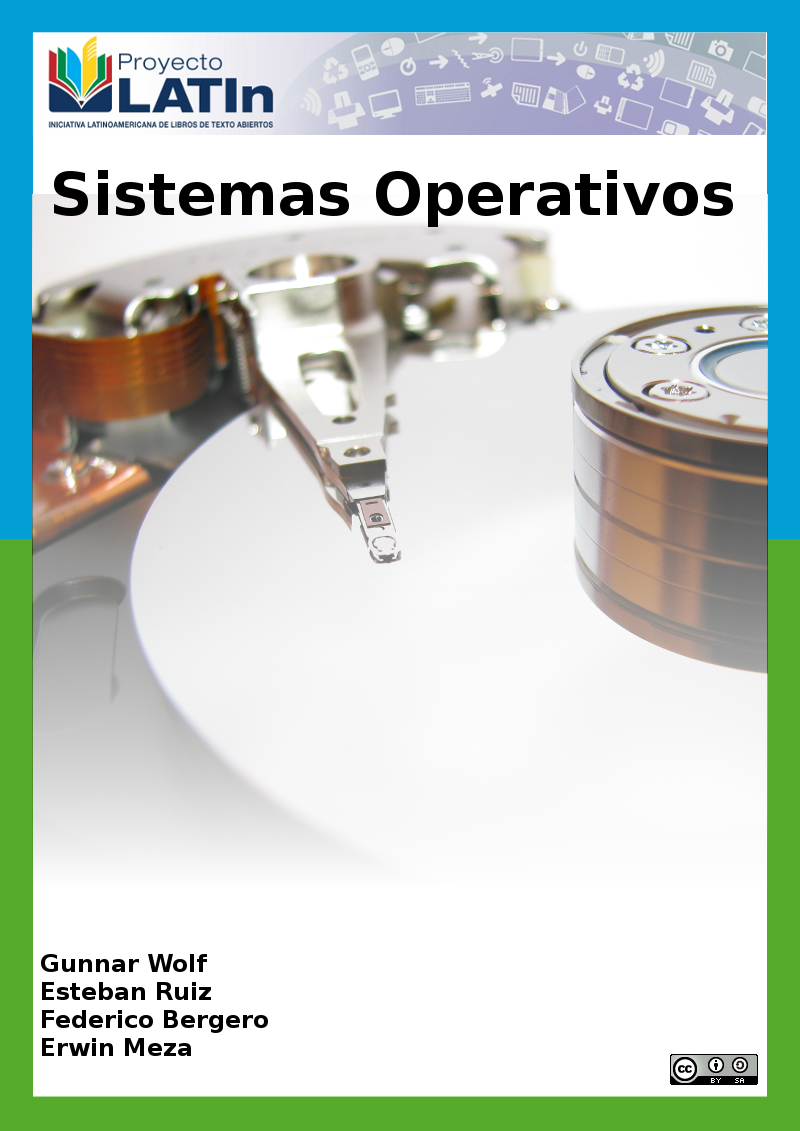
\includepdf{portada.png} %en esta imagen deben ir los nombres de los autores






%----------------------------------------------------------------------------------------
%	COPYRIGHT PAGE
%----------------------------------------------------------------------------------------
\pagestyle{empty} 
latin/primerapag.tex
%----------------------------------------------------------------------------------------
%	TABLE OF CONTENTS
%----------------------------------------------------------------------------------------

%\chapterimage{chapter_head_1.pdf} % Table of contents heading image
\chapterimage{cabecera.jpg}
\pagestyle{empty} % No headers

\tableofcontents % Print the table of contents itself

\cleardoublepage % Forces the first chapter to start on an odd page so it's on the right

\pagestyle{fancy} % Print headers again










%\maketitle

%\setcounter{tocdepth}{2}
%\tableofcontents
%\vspace*{1cm}

\chapter{Presentación}
\addcontentsline{toc}{chapter}{Presentación}

\section{Acerca del libro}
\chaptermark{Presentación}

Este libro busca brindar a estudiantes y docentes de las carreras de
\emph{Ingeniería en Computación}, \emph{Informática}, \emph{Ciencias de la Computación} y similares un material completo, general y autocontenido
sobre la materia de \emph{Sistemas Operativos}. No se asume conocimiento
previo sobre la temática, aunque se utilizarán conceptos de
estructuras de datos y algoritmos básicos.

\section*{Justificación}

Actualmente existe vasta bibliografía sobre Sistemas Operativos, sin
embargo la gran mayoría está escrita en inglés, y cuando están
disponibles en castellano, su traducción deja mucho que desear,
llevando a conceptos confusos y difíciles de comprender. La intención
de los autores es que el presente texto provea un material redactado
originalmente en castellano, revisado por docentes latinoamericanos
utilizando la terminología más adecuada para los alumnos de la región
y eliminando muchos de los errores de traducción.

Generalmente el material de cursos de Sistemas Operativos está
compuesto por partes de distintos libros, artículos de investigación,
recursos en linea, software, ejercitación, etc. Por ello, el alumno
debe recurrir a distintas fuentes durante el curso. El presente
libro pretende ser de utilidad tanto para alumnos como para
docentes como una única publicación autocontenida. Cabe remarcar
también que el material bibliográfico generalmente está protegido por
derecho de autor, es costoso y en muchos casos de dificil acceso
(sobre todo las publicaciones en inglés).

Los contenidos de la bibliografía clásica de Sistemas Operativos están
basadas en re-ediciones y compendio de libros de hace varias décadas
que incluyen temas obsoletos o desactualizados. Existen también
desarrollos y tendencias nuevas en el área que aun no han sido
integradas en la bibliografía clásica, y mucho menos a las
traducciones. El presente libro pretende también revisar y actualizar
los conceptos clásicos de sistemas operativos inlcuyendo material de
publicación reciente.

Este libro se desarrolló dentro del marco del \href{http://www.latinproject.org}{Proyecto LATIn}, enfocado a
la creación de libros de texto con un esquema de licenciamiento libre,
derivados de la creación y colaboración de grupos de trabajo
multinacionales, para la región latinoamericana.


\section*{Público objetivo}

Este libro está apuntado tanto a estudiantes de carreras de informática, 
computación e ingenierías como a los aficionados de la computadora
interesados en conocer un poco más de lo que realmente ocurre dentro 
de un sistema de cómputo y el rol que cumple el sistema operativo.

Al finalizar el libro se espera que el lector haya adquirido conocimientos
y habilidades como:

\begin{itemize}
\item Administrar, diseñar y desarrollar un sistema operativo.
\item Conociendo el funcionamiento general de los sistemas operativos,
      poder sacar mejor provecho de la computadora
\item Conocer y saber aprovechar no sólo los sistemas, sino las
   metodologías y principales formas de interacción del software libre
\end{itemize}
 
Se asume también que el lector está familiarizado 
con algún lenguaje de programación
de alto nivel, y –al menos a nivel básico– con C.
Aunque los ejemplos de código están dados en diversos lenguajes de programación
(Bash, Perl, c, PascalFC, Python, Ruby, Ensamblador, entre otros), éstos
son tan sencillos que pueden ser fácilmente escritos en el lenguaje 
de elección del lector sin mayor esfuerzo.

Resultará muy conveniente que tener acceso a una computadora con
sistema operativo Linux (GNU) u otro Unix libre. 

\section*{Estructura temática}

El texto comprende los siguientes capítulos:

\begin{description}
\item[1. Introducción] Para comenzar a hablar de sistemas operativos, es
                  necesario en primer término enmarcar \emph{qué es} un
                  sistema operativo y cuáles son sus funciones
                  principales. También es importante detallar algunos
                  puntos que, contrario a la percepción común, \emph{no                   pueden} considerarse parte de sus funciones.

		  Este tema se presenta apoyado de la evolución
                  histórica del cómputo, haciendo énfasis en por qué
                  este proceso evolutivo en particular desembocó en
                  los sistemas operativos que existen hoy en día.
\item[2. Relación con el hardware] Partiendo de que una de las
     principales tareas del sistema operativo es presentar una
     \emph{abstracción regular} del hardware a los procesos que se
     ejecuten, resulta importante presentar cómo éste está
     estructurado, y cómo el sistema operativo puede comunicarse con
     él.

     Este capítulo aborda la \emph{jerarquía de almacenamiento}, el
     mecanismo de \emph{interrupciones} y \emph{excepciones} y el papel que
     juegan para las \emph{llamadas al sistema}, las características base
     de diversos tipos de dispositivo del sistema, el concepto de
     \emph{canales} (o \emph{buses}) de comunicación, el mecanismo de \emph{acceso      directo a memoria}, y una introducción a lo que puede ser visto
     como tema conductor a lo largo de todo el libro: La importancia
     y complejidad de la \emph{concurrencia}, y su relación con el
     \emph{paralelismo} y \emph{multiprocesamiento}.
\item[3. Administración de procesos] La entidad principal con la que
     interactúa un sistema operativo (sea para brindarle servicios o
     para imponerle restricciones) es el proceso. Este capítulo inicia
     presentando los diferentes estados de los procesos y la relación
     entre éstas y sus \emph{hermanos menores} (los \emph{hilos}), y los
     principales modelos empleados para el multiprocesamiento.

     Todos los sistemas operativos modernos tienen que enfrentar a la
     \emph{concurrencia}: La incertidumbre del ordenamiento en el tiempo
     entre eventos relativos a los diferentes procesos e hilos. La
     parte medular de este capítulo presenta a las \emph{primitivas de      sincronización}: Mutexes, semáforos y monitores. Para
     ilustrarlas, se emplean los patrones y problemas clásicos que se
     han seguido a lo largo de su desarrollo histórico.

     Pero las primitivas pueden sólamente utilizarse entre procesos
     que \emph{cooperan deliberadamente} entre sí. Un sistema operativo
     debe implementar protección y separación incluso entre procesos
     que \emph{compiten} o que sencillamente no saben el uno acerca del
     otro. Por ello, la última sección de este capítulo aborda los
     diferentes mecanismos que existen para evitar las situaciones de
     \emph{bloqueo mutuo}.
\item[4. Planificación de procesos] Para que varios procesos coexistan
     en un sistema de cómputo, el primer recurso que el sistema
     operativo debe \emph{multiplexar} o repartir entre todos ellos es el tiempo de
     cómputo: El uso del procesador. Este capítulo presenta los
     diferentes niveles de \emph{planificador} que forman parte de un
     sistema operativo, y analiza al \emph{planificador a corto plazo}
     (también conocido como \emph{despachador}). Se presentan los
     principales algoritmos, y se ilustra cómo los sistemas operativos
     modernos van empleando técnicas mixtas de varios de ellos.

     Por último, se abordan tres temas brevemente: Los diferentes
     modelos de planificación de hilos y su relación
     con los procesos, las particularidades de la planificación en un
     entorno con multiprocesadores reales, y las necesidades de
     planificación de \emph{tiempo real}.
\item[5. Administración de memoria] Los \emph{programas} sólo se vuelven
     procesos cuando se les asigna memoria y tiempo de cómputo: Cuando dejan de ser el
     resultado de una compilación guardada estáticamente para
     convertirse en una entidad dinámica. Este capítulo presenta en
     primer lugar la visión \emph{desde dentro} de la memoria por parte de
     cada uno de los procesos: El espacio de direccionamiento y el
     acomodo clásico de las regiones de un proceso en la memoria que
     le es asignada.

     Para que los distintos procesos compartan la memoria del sistema,
     a lo largo de la historia se han presentado diferentes
     esquemas. Se presentan someramente los esquemas de partición
     contigua fija y variable, para profundizar posteriormente en los
     que ofrecen mayor flexibilidad al sistema operativo y se
     mantienen en uso al día de hoy: La segmentación y la
     paginación. De esta última, se continúa para presentar la
     abstracción que ha liberado a los sistemas operativos para
     \emph{sobrecomprometer} la memoria de forma eficiente y prácticamente
     transparente: La memoria virtual.

     Al manejar la memoria de un proceso surgen puntos importantes a
     tomar en cuenta en lo relativo a la seguridad en cómputo; la
     parte final de este capítulo presenta la vulnerabilidad conocida
     como \emph{desbordamiento de pila} (\emph{buffer overflow}), y algunas
     estrategias de mitigación que se han implementado con el paso de
     los años para mitigar su peligrosidad.
\item[6. Organización de archivos] De cara al usuario, probablemente la
     principal abstracción implementada por el sistema operativo es la
     organización de la información sobre un medio persistente. Hoy en
     día, la norma es que esta organización se realice en \emph{archivos}
     estructurados sobre una estructura jerárquica llamada
     \emph{directorio}. Este capítulo se centra en explicar esta
     abstracción, sin entrar aún en detalles respecto a cómo se llega
     a un respaldo físico de la misma.

     Estos conceptos parecen tan pervasivos y universales que podría
     pensarse que no requieren mayor análisis. Sin embargo, resulta
     importante abordar las diferencias semánticas derivadas del
     desarrollo histórico de distintos sistemas. En este capítulo se
     presentan varios conceptos cuya implementación en un medio que
     asegure la persistencia se describirá en el siguiente capítulo.

     Por último, en este capítulo se incluye un breve repaso de
     distintos tipos de sistemas de archivos en red, enfatizando
     nuevamente en los cambios semánticos derivados de la distinta
     historia de cada implementación.
\item[7. Sistemas de archivos] Este capítulo presenta la contraparte
     obligada del anterior: ¿Cómo se estructuran los dispositivos de
     almacenamiento a largo plazo, a los cuales nos referimos
     genéricamente como \emph{discos}? ¿Cómo se van plasmando las
     estructuras mediante las cuales el usuario organiza la
     información en bloques dentro de un dispositivo? ¿Qué problemas
     pueden derivar del uso de estos \emph{sistemas de archivos}, y qué
     métodos para evitarlos o resolverlos se han implementado?

     La parte central de este capítulo se centra en un sistema de
     archivos bastante viejo y simple, pero aún en muy amplio uso en el cómputo
     moderno: La familia \emph{FAT}.
\end{description}

Los siguientes temas resultan muy importantes para la comprensión y
para el desarrollo futuro de la materia, pero dado que son \emph{empleados}
por el sistema operativo (y no necesariamente son \emph{parte integral} del
mismo), se presentan como apéndices

\begin{description}
\item[A. Software libre y licenciamiento] Estudiar sistemas operativos
     cruza necesariamente la temática del \emph{software libre}. Uno de los
     principios fundamentales del desarrollo histórico es la \emph{libertad      de aprender}, esto es, todo software que se diga \emph{libre} debe
     permitir a sus usuarios comprender sus estructuras básicas, la
     relación entre ellas, y la lógica general de su programación.

     Hoy en día existe una gran cantidad de sistemas operativos
     libres, tanto de propósito general como enfocados a un nicho. El
     \emph{movimiento ideológico} del software libre, contrario a cualquier
     pronóstico que pudiera haberse hecho al iniciarse en 1984,
     claramente ha cambiado el desarrollo del cómputo. Todos los
     sistemas operativos que pueden ser estudiados \emph{de primera mano},
     constatando la implementación de sus principios son
     necesariamente (aunque con una definición ligeramente laxa)
     software libre.

     Hacia el año 2000 se fue haciendo claro que estas ideas no pueden
     aplicarse únicamente al software. Poco a poco fue definiéndose
     una noción mucho más amplia, la de los \emph{bienes culturales      libres}. El presente libro busca ser una contribución a esta
     última categoría.

     El primer apéndice aborda brevemente estos temas, así como los
     principales modelos de licenciamiento libre utilizados.
\item[B. Virtualización] La virtualización es una herramienta muy útil,
     y cada vez más al alcance de todos, para el aprendizaje de los
     sistemas operativos. Hay una gran cantidad de recursos para
     comprender desde los primeros momentos del arranque de la
     computadora. Empleando imágenes de máquinas virtuales, pueden
     comprenderse y desmenuzarse los distintos elementos del sistema
     operativo, e incluso observar el resultado de realizar
     modificaciones sobre un sistema operativo real. Es, por tanto,
     una herramienta muy importante para acompañar al aprendizaje de
     esta materia.

     La virtualización es también una tecnología que permea cada vez
     más aspectos del uso profesional del cómputo, y comprenderlo
     ayudará al lector a elegir las herramientas específicas a
     emplear.

     Pero hablar de \emph{la virtualización} como un todo ignoraría
     aspectos fundamentales de la riqueza que presenta este campo. Al
     igual que con los conceptos presentados a lo largo del libro, la
     virtualización es presentada a partir de su perspectiva
     histórica, y detallando hacia las distintas modalidades que se
     han desarrollado al paso del tiempo.
\item[C. El medio físico y el almacenamiento] En el capítulo \ref{sec-7} se
     presenta cómo se \emph{concretiza} la abstracción de archivos y
     directorios para plasmarlo en un gran arreglo lineal de datos, en
     una entidad aún abstracta a la cual se sigue haciendo referencia
     con el nombre genérico de \emph{disco}. Este apéndice se ocupa de los
     detalles físicos del acomodo de la información en su medio.

     Pero un \emph{disco} va mucho más allá de un dispositivo que
     simplemente vuelca dicho arreglo a un medio persistente. En
     primer término, los \emph{discos magnéticos rotativos} (el medio
     dominante de almacenamiento) presentan peculiaridades que los
     sistemas operativos tuvieron que saber resolver. El desarrollo de
     la tecnología, sin embargo, fue \emph{arrebatando} estas áreas del
     ámbito del sistema operativo, entregándolas a la optimización
     realizada dentro del \emph{hardware controlador}.

     Por otro lado, la tecnología de \emph{almacenamiento en estado sólido}
     ha llegado a niveles de madurez que en determinados mercados ya
     la colocan claramente por encima de los discos magnéticos. Esto
     implica cambios importantes para el modo en que el sistema
     operativo debe estructurar y modificar la información.

     Por último, un \emph{volumen} ya no necesariamente se refiere a un
     único medio físico. Este apéndice aborda tanto a \emph{RAID}, el
     primer mecanismo que se popularizó para \emph{agregar} varias unidades
     para mejorar tanto la capacidad máxima y la confiabilidad de un
     volumen, como al manejo avanzado de volúmenes, en que el sistema
     operativo incorpora la lógica de RAID con la del manejo de
     sistemas de archivos para lograr mucho mayor flexibilidad.
\end{description}

\section*{Licenciamiento}

Este libro fue desarrollado como parte del \href{http://www.latinproject.org/}{Proyecto LATIn}, que busca
la creación de libros de texto \emph{libres} para nivel universitario, y
enfocado a Latinoamérica.

Cualquier porción de este libro puede ser reproducido y utilizado para
todo fin, bajo los términos de la licencia \emph{\href{https://creativecommons.org/licenses/by-sa/4.0/deed.es}{Creative Commons-Atribución-CompartirIgual}} (\emph{CC-BY-SA}) versión 4.0.

Este modelo de licenciamiento se presenta y explica en la sección
\ref{SL_CC}.


\chapter{Introducción}
\label{sec-1}
\section{¿Qué es un sistema operativo?}
\label{sec-1-1}
\label{INTRO}


El \emph{sistema operativo} es el principal programa que se ejecuta en toda
computadora de propósito general.

Hay sistemas operativos de todo tipo, desde muy simples hasta
terriblemente complejos, y entre más casos de uso hay para el cómputo
en la vida diaria, más variedad habrá en ellos.

No nos referiremos al sistema operativo como lo ve el usuario final, o
como lo vende la mercadotecnia — El ambiente gráfico, los programas
que se ejecutan en éste, los lenguajes de programación en que están 
desarrollados y en que más fácilmente se puede desarrollar para ellos, 
e incluso el conjunto básico de funciones que las bibliotecas base ofrecen son
principalmente \emph{clientes} del sistema operativo — Se ejecutan sobre él, y
ofrecen su implementación a sus usuarios (incluídos, claro, los
desarrolladores). La diferencia en el uso son sólo –y si mucho–
\emph{consecuencias} del diseño de un sistema operativo. Más aún, con el
mismo sistema operativo –como pueden constatarlo comparando dos
distribuciones de Linux, o incluso la forma de trabajo de dos usuarios
en la misma computadora– es posible tener \emph{entornos operativos}
completamente disímiles.
\subsection{¿Por qué estudiar los sistemas operativos?}
\label{sec-1-1-1}


La importancia de estudiar este tema radica no sólo en comprender los
mecanismos que emplean los sistemas operativos para cumplir sus tareas
sino en entender estos mecanismos para evitar los errores más
comunes al programar, que pueden resultar desde un rendimiento
deficiente hasta pérdida de información.

Como desarrolladores, comprender el funcionamiento básico de los
sistemas operativos y las principales alternativas que nos ofrecen en
muchos de sus puntos, o saber diseñar algoritmos y procesos que se ajusten
mejor al sistema operativo en que vayamos a ejecutarlo, puede resultar
en una diferencia cualitativa decisiva en nuestros productos.

Como administradores de sistemas, muchas veces podemos enfrentarnos a
situaciones de bajo rendimiento, de conflictos entre aplicaciones,
demoras en la ejecución, y comprender lo que ocurre \emph{tras bambalinas}
resulta fundamental para realizar nuestro trabajo. Los sistemas de
archivos resultan un área de especial interés para administradores de
sistemas: ¿Cómo comparar las virtudes y desventajas de tantos sistemas
existentes? ¿Por qué puede resultarnos conveniente mezclarlos en el
mismo servidor? ¿Cómo evitar la corrupción o pérdida de información?
Lo que es más, ¿cómo recuperar información de un disco dañado?

En el área de la seguridad en cómputo, la relación resulta obvia:
si nos interesa localizar vulnerabilidades que nos permitan elevar
nuestro nivel de privilegios, ¿cómo podríamos hacerlo sin comprender
cómo se engranan los diversos componentes de un sistema? La cantidad
de tareas que debe cubrir un sistema operativo es tremenda, y veremos
ejemplos de sitios donde un atacante puede enfocar sus energías. Del
mismo modo, para quien busca \emph{defender} un sistema (o una red), resulta
fundamental comprender cuáles son los vectores de ataque más comunes y
–nuevamente– la relación entre los componentes involucrados para poder
remediar o, mejor, prevenir dichos ataques.

Y claro está, podemos ver al mundo en general, fuera del entorno del
cómputo, como una serie de modelos interactuantes. Muchos de los
métodos y algoritmos que aquí veremos pueden emplearse fuera del
entorno del cómputo, y una vez que comprendamos los problemas de
concurrencia, de competencia por recursos, o de protección y separación
que han sido resueltos en el campo de los sistemas operativos, podemos
extrapolar estas soluciones a otros campos.

El camino por delante es largo, y puede resultar interesante y divertido.
\section{Funciones y objetivos de los sistemas operativos}
\label{sec-1-2}


El sistema operativo es el único programa que interactúa directamente
con el hardware de la computadora. Sus funciones primarias son:

\begin{description}
\item[Abstracción] Los programas no deben tener que preocuparse de los
                 detalles de acceso a hardware, o de la configuración
                 particular de una computadora. El sistema operativo
                 se encarga de proporcionar una serie de abstracciones
                 para que los programadores puedan enfocarse en
                 resolver las necesidades particulares de sus
                 usuarios. Un ejemplo de tales abstracciones es que
                 la información está organizada en \emph{archivos} y
                 \emph{directorios} (en uno o muchos \emph{dispositivos de                  almacenamiento}).
\item[Administración de recursos] Una sistema de cómputo puede tener a su
     disposición una gran cantidad de \emph{recursos} (memoria, espacio de
     almacenamiento, tiempo de procesamiento, etc.), y los diferentes
     \emph{procesos} que se ejecuten en él \emph{compiten} por ellos. Al gestionar
     toda la asignación de recursos, el sistema operativo puede
     implementar políticas que los asignen de forma efectiva y acorde
     a las necesidades establecidas para dicho sistema.
\item[Aislamiento] En un sistema multiusuario y multitarea cada proceso 
		 y cada usuario no tendrá que
                 preocuparse por otros que estén usando el mismo
                 sistema — Idealmente, su \emph{experiencia} será la misma
                 que si el sistema estuviera exclusivamente dedicado a
                 su atención (aunque fuera un sistema menos
                 poderoso).

		 Para implementar correctamente las funciones de
		 aislamiento hace falta que el sistema operativo
		 utilice hardware específico para dicha protección.
\end{description}
\section{Evolución de los sistemas operativos}
\label{sec-1-3}


No se puede comenzar a abordar el tema de los sistemas operativos sin
revisar brevemente su desarrollo histórico. Esto no sólo permitirá
comprender por qué fueron apareciendo determinadas características y
patrones de diseño que se siguen empleando décadas más tarde, sino
(como resulta particularmente bien ejemplificado en el discurso de
recepción del premio Turing de Fernando Corbató en 1990, \emph{\href{http://dl.acm.org/citation.cfm?id=1283947}{On building systems that will fail}}), adecuar un sistema existente a un entorno
cambiante, por mejor diseñado que éste estuviera, lleva casi
inevitablemente a abrir espacios de comportamiento no previsto — El
espacio más propicio para que florezcan los fallos. Conocer los
factores que motivaron a los distintos desarrollos puede ayudar a
prever y prevenir problemas.
\subsection{Proceso por lotes (\emph{batch processing})}
\label{sec-1-3-1}


Los antecedentes a lo que hoy se conoce como sistema operativo
se pueden encontrarlos en la automatización inicial del procesamiento de
diferentes programas, surgida en los primeros centros de
cómputo: cuando en los `50 aparecieron los dispositivos
perforadores/lectores de tarjetas de papel, el tiempo que una
computadora estaba improductiva esperando a que estuviera lista una
\emph{tarea} (como se designaba a una ejecución de cada determinado
programa) para poder ejecutarla disminuyó fuertemente ya que los programadores
entregaban su lote de tarjetas perforadas (en inglés,
batches) a los operadores, quienes las alimentaban a los dispositivos
lectores, que lo cargaban en memoria en un tiempo razonable, iniciaban
y monitoreaban la ejecución, y producían los resultados.

En esta primer época en que las computadoras se especializaban en
tareas de cálculo intensivo y los dispositivos que interactuaban con
medios externos eran prácticamente desconocidos, el rol del sistema
\emph{monitor} o \emph{de control} era básicamente asistir al operador en la
carga de los programas y las bibliotecas requeridas, la notificación
de resultados y la contabilidad de recursos empleados para su cobro.

Los sistemas monitores se fueron sofisticando al implementar
protecciones que evitaran la corrupción de \emph{otros trabajos} (por
ejemplo, lanzar erróneamente la instrucción \emph{leer siguiente tarjeta}
causaría que el siguiente trabajo encolado perdiera sus primeros
caracteres, corrompiéndolo e impidiendo su ejecución), o que entraran
en un ciclo infinito, estableciendo \emph{alarmas} (\emph{timers}) que
interrumpirían la ejecución de un proceso si éste duraba más allá del
tiempo estipulado. Estos monitores implicaban la modificación del
hardware para contemplar dichas características de seguridad — Y ahí
se puede hablar ya de la característica básica de gestión de recursos
que identifica a los sistemas operativos.

Cabe añadir que el tiempo de carga y puesta a punto de una tarea
seguía representando una parte importante del tiempo que la
computadora dedicaba al procesamiento: un lector de cintas rápido procesaba
del orden de cientos de caracteres por minuto, y a pesar de la
lentitud relativa de las computadoras de los `50 ante los estándares
de hoy (se medirían por miles de instrucciones por segundo, KHz, en
vez de miles de millones como se hace hoy, GHz), esperar cinco o
diez minutos con el sistema completamente detenido por la carga de un
programa moderadadamente extenso resulta a todas luces un desperdicio.
\subsection{Sistemas en lotes con dispositivos de carga (\emph{spool})}
\label{sec-1-3-2}


Una mejora natural a este último punto fue la invención del \emph{spool}:
Un mecanismo de entrada/salida que permitía que una computadora de
propósito específico, mucho más económica y limitada, leyera las
tarjetas y las fuera convirtiendo a cinta magnética, un medio mucho
más rápido, teniéndola lista para que la computadora central la
cargara cuando terminara con el trabajo anterior. Del mismo modo, la
computadora central guardarba sus resultados en cinta para que equipos
especializados la leyeran e imprimieran para el usuario solicitante.

La palabra \emph{spool} (\emph{bobina}) se tomó como \emph{acrónimo inverso} hacia
\emph{Simultaneous Peripherial Operations On-Line}, \emph{operación simultánea de periféricos en línea}.
\subsection{Sistemas multiprogramados}
\label{sec-1-3-3}
\label{INTRO_multiprogramados}


A lo largo de su ejecución, un programa normalmente pasa por etapas
con muy distintas características: durante un ciclo fuertemente
dedicado al cálculo numérico, el sistema opera \emph{limitado por el CPU}
(\emph{CPU-bound}), mientras que al leer o escribir resultados a medios
externos (incluso a través de \emph{spools}) el límite es impuesto por los
dispositivos, esto es, opera \emph{limitado por entrada-salida} (\emph{I-O bound}). La \emph{programación multitareas} o los \emph{sistemas multiprogramados} buscaban maximizar el tiempo de uso efectivo
del procesador ejecutando varios procesos al mismo tiempo.

El hardware requerido cambió fuertemente. Si bien se esperaba que cada
usuario fuera responsable con el uso de recursos, se hizo necesario
que apareciera la infraestructura de protección de recursos: un
proceso no debe sobreescribir el espacio de memoria de otro (ni el
código ni los datos), mucho menos el espacio del monitor. Esta
protección  se encuentra en la \emph{Unidad de Manejo de Memoria} (MMU),
presente en todas las computadoras de uso genérico desde los `90.

Ciertos dispositivos requieren bloqueo para ofrecer acceso
exclusivo/único — Cintas e impresoras, por ejemplo, son de acceso
estrictamente secuencial, y si dos usuarios intentaran usarlas al
mismo tiempo, el resultado para ambos se corrompería. Para estos
dispositivos, el sistema debe implementar otros \emph{spools} y mecanismos
de bloqueo.
\subsection{Sistemas de tiempo compartido}
\label{sec-1-3-4}


El modo de interactuar con las computadoras se modificó drásticamente
durante los `60, al extenderse la multitarea para
convertirse en sistemas \emph{interactivos} y \emph{multiusuarios}, en buena
medida diferenciados de los anteriores por la aparición de las
\emph{terminales} (primero teletipos seriales, posteriormente equipos con
una pantalla completa como se conocen hasta hoy).

En primer término, la tarea de programación y depuración del código se
simplificó fuertemente al poder el programador hacer directamente
cambios y someter el programa a la ejecución inmediata. En segundo
término, la computadora \emph{nunca más estaría simplemente esperando a que esté listo un progama}: Mientras un programador editaba o compilaba su programa,
la computadora seguía calculando lo que otros procesos requirieran.

Un cambio fundamental entre el modelo de \emph{multiprogramación} y de
\emph{tiempo compartido} es el tipo de control sobre la multitarea:
(se verá en detalle en el capítulo \ref{sec-3} (\emph{Administración de procesos})

\begin{description}
\item[Multitarea \emph{cooperativa} o \emph{no apropiativa}] (\emph{Cooperative      multitasking}) La implementaron los sistemas multiprogramados: Cada
     proceso tenía control del CPU hasta que éste hacía una llamada al
     sistema (o indicara su \emph{disposición a cooperar} por medio de la
     llamada \texttt{yield}: \emph{ceder el paso}).

     Un cálculo largo no era interrumpido por el sistema operativo,
     en consecuencia un error de programador podía congelar la
     computadora completa.
\item[Multitarea \emph{preventiva} o \emph{apropiativa}] (\emph{Preemptive      multitasking}) En los sistemas de tiempo compartido, el reloj del
     sistema interrumpe periódicamente a los diversos procesos,
     transfiriendo \emph{forzosamente} el control nuevamente al sistema
     operativo. El sistema operativo puede entonces elegir 
     otro proceso para continuar la ejecución.
\end{description}

Además, fueron naciendo de forma natural y paulatina las abstracciones
que se conocen hoy en día, como los conceptos de \emph{archivos} y
\emph{directorios}, y el código necesario para emplearlos iba siendo
enviado a las \emph{bibliotecas de sistema} y, cada vez más (por
su centralidad) hacia el núcleo mismo del –ahora sí– sistema
operativo.

Un cambio importante
entre los sistemas multiprogramados y de tiempo compartido es que la
velocidad del cambio entre una tarea y otra es mucho más rápido: si
bien en un sistema multiprogramado un \emph{cambio de contexto} podía
producirse sólo cuando la tarea cambiaba de un modo de
ejecución a otro, en un sistema interactivo, para dar la \emph{ilusión} de uso exclusivo de la
computadora, el hardware emitía periódicamente al sistema operativo
\emph{interrupciones} (señales) que le indicaban que cambie el \emph{proceso} activo 
(como ahora se le denomina a una instancia de un programa en ejecución).

Diferentes tipos de proceso pueden tener distinto nivel de importancia
— Ya sea porque son más relevantes para el funcionamiento de la
computadora misma (procesos de sistema), porque tienen mayor carga de
interactividad (por la experiencia del usuario) o por diversas
categorías de usuarios (sistemas con contabilidad por tipo de
atención). Esto requiere la implementación de diversas \emph{prioridades}
para cada uno de estos.
\section{Y del lado de las computadoras personales}
\label{sec-1-4}
\label{INTRO_computadoras_personales}


Si bien la discusión hasta este momento asume una computadora central
con operadores dedicados y múltiples usuarios, en la década de los
`70 comenzaron a aparecer las \emph{computadoras personales}, sistemas en
un inicio verdaderamente reducidos en prestaciones y a un nivel de
precios que los ponían al alcance, primero, de los aficionados
entusiastas y, posteriormente, de cualquiera.
\subsection{Primeros sistemas para entusiastas}
\label{sec-1-4-1}


\begin{figure}[htb]
\centering
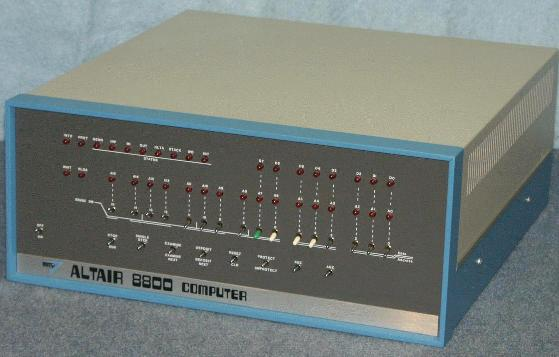
\includegraphics[width=0.5\textwidth]{./img/altair.jpg}
\caption{\label{INTRO_altair}La \emph{microcomputadora Altair 8800}, primer computadora personal con distribución masiva, a la venta a partir de 1975. (Imagen de la Wikipedia: \emph{Altair 8800})}
\end{figure}

Las primeras computadoras personales eran distribuídas sin 
sistemas operativos o lenguajes de programación; la interfaz primaria
para programarlas era a través de llaves (\emph{switches}), y para recibir sus
resultados, se utilizaban bancos de LEDs. Claro está, esto requería conocimientos
especializados, y las computadoras personales eran aún vistas sólo
como juguetes caros.
\subsection{La revolución de los 8 bits}
\label{sec-1-4-2}


La verdadera revolución apareció cuando‚ poco tiempo más tarde,
comenzaron a venderse computadoras personales con salida de video
(típicamente a través de una televisión) y entrada a través de un
teclado. Estas computadoras popularizaron el lenguaje de programación
BASIC, diseñado para usuarios novatos en los `60, y para permitir a
los usuarios gestionar sus recursos (unidades de cinta, pantalla
posicionable, unidades de disco, impresoras, modem, etc.) llevaban un
software mínimo de sistema — Nuevamente, un proto-sistema operativo.

\begin{figure}[htb]
\centering
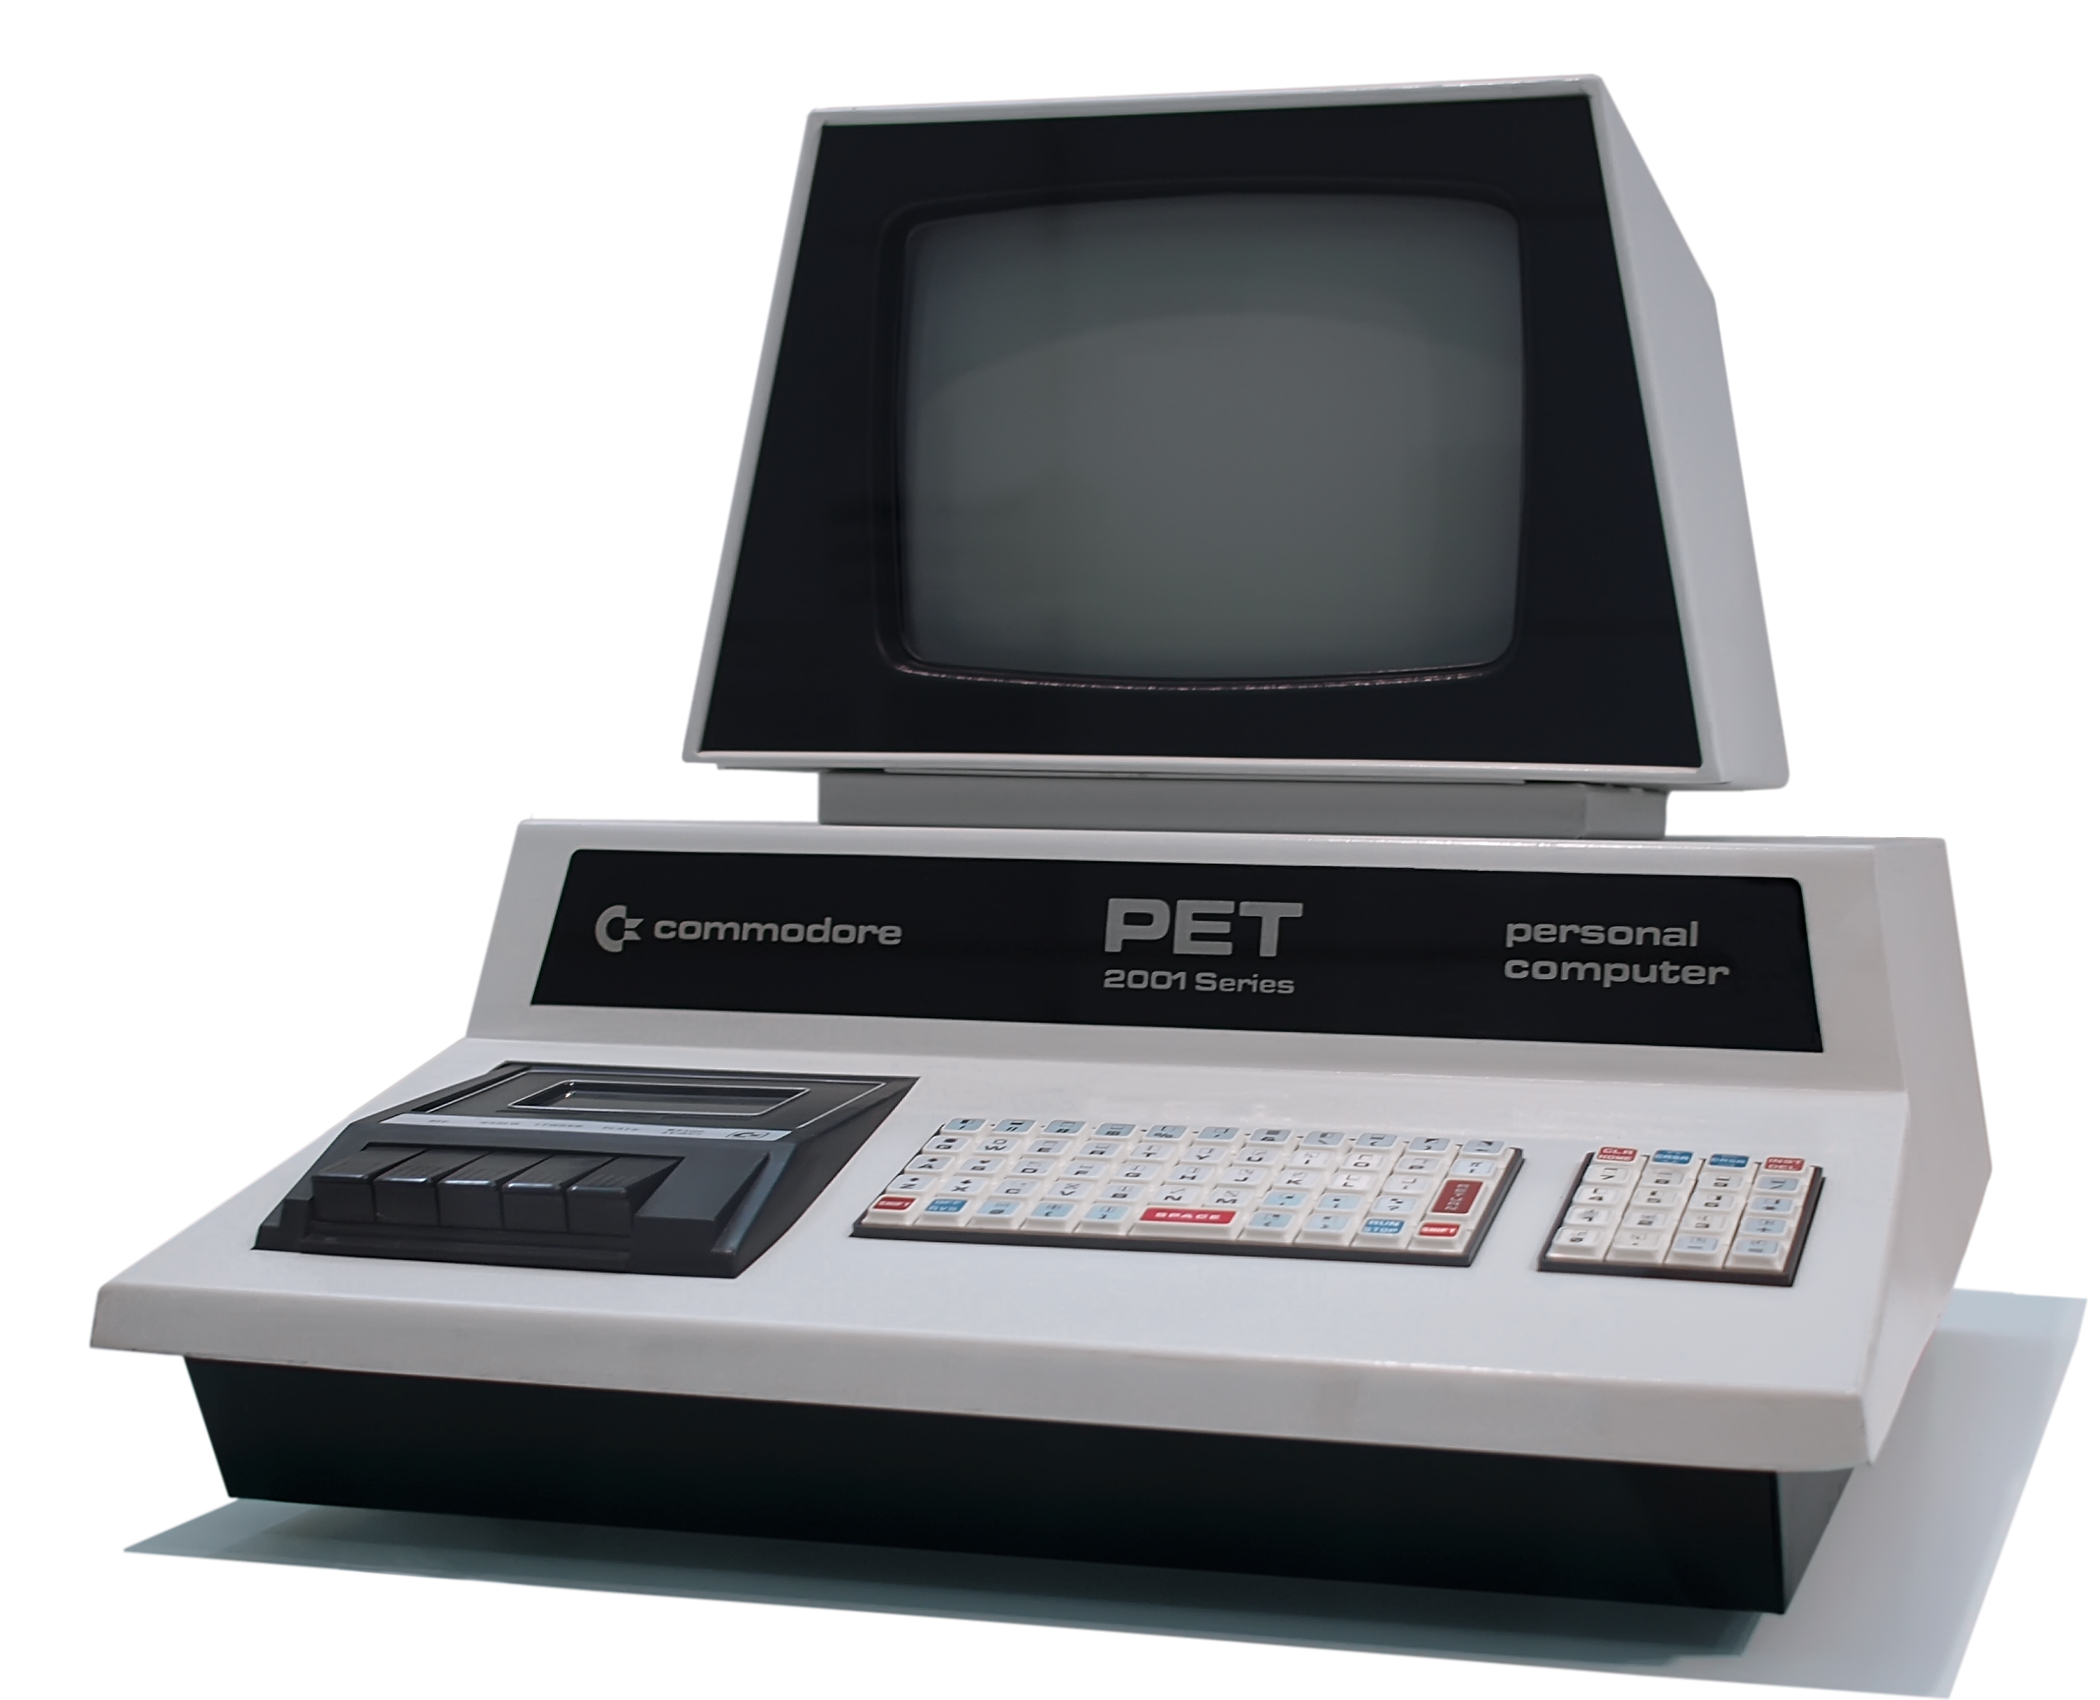
\includegraphics[width=0.5\textwidth]{./img/commodore_pet.jpg}
\caption{\label{INTRO_commodore_pet}La \emph{Commodore Pet 2001}, en el mercado desde 1977, una de las primeras con intérprete de BASIC. (Imagen de la Wikipedia: \emph{Commodore PET})}
\end{figure}
\subsection{La computadora para fines ``serios'': La familia PC}
\label{sec-1-4-3}


Al aparecer las computadoras personales ``serias'', orientadas a la
oficina más que al hobby, a principios de los `80 (particularmente
representadas por la IBM PC, 1981), sus sistemas operativos se
comenzaron a diferenciar de los equipos previos al separar el \emph{entorno de desarrollo} en algún lenguaje de programación del \emph{entorno de ejecución}. El rol principal del sistema operativo ante el usuario era
administrar los archivos de las diversas aplicaciones a
través de una sencilla interfaz de línea de comando, y lanzar las
aplicaciones que el usuario seleccionaba.

La PC de IBM fue la primer arquitectura de computadoras personales en
desarrollar una amplia familia de \emph{clones}, computadoras compatibles
diseñadas para trabajar con el mismo sistema operativo, y que
eventualmente capturaron casi el 100\% del
mercado. Prácticamente todas las computadoras de escritorio y
portátiles en el mercado hoy derivan de la arquitectura de la IBM PC.

\begin{figure}[htb]
\centering
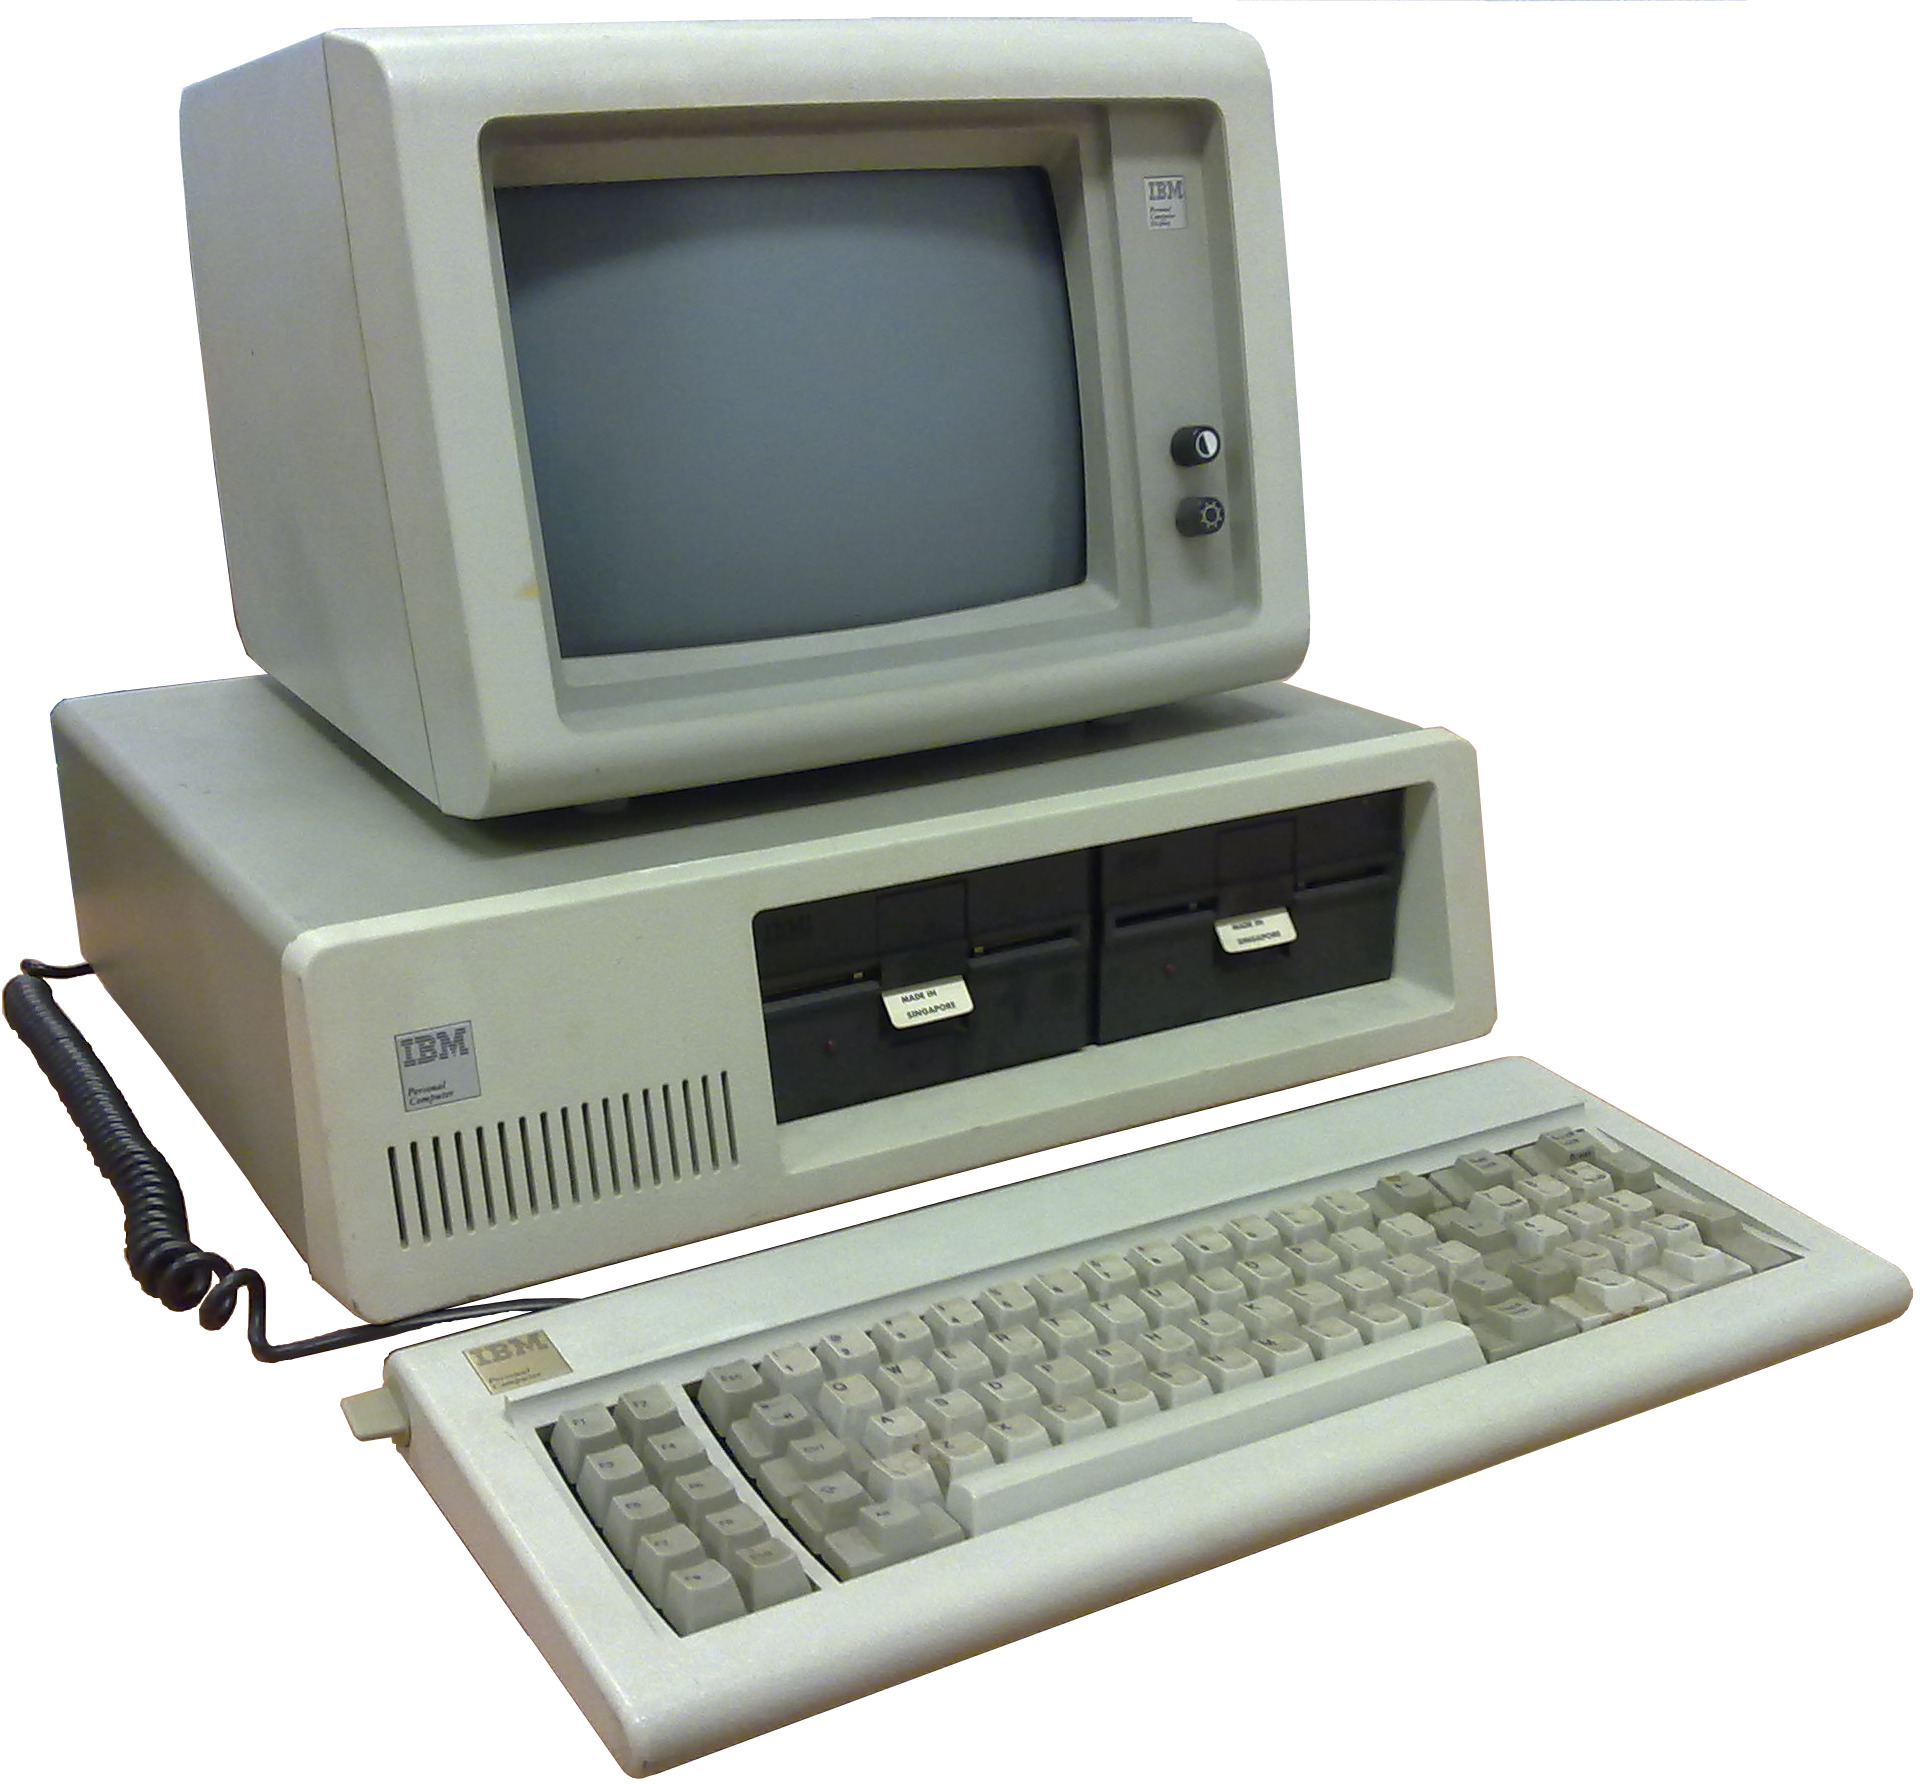
\includegraphics[width=0.5\textwidth]{./img/ibmpc.jpg}
\caption{\label{INTRO_ibmpc}La computadora IBM PC modelo 5150 (1981), iniciadora de la arquitectura predominantemente en uso hasta el día de hoy. (Imagen de la Wikipedia: \emph{IBM Personal Computer})}
\end{figure}

Ante las aplicaciones, el sistema operativo (PC-DOS, en las versiones
distribuídas directamente por IBM, o el que se popularizó más, MS-DOS,
en los \emph{clones}) ofrecía la ya conocida serie de interfaces y
abstracciones para administrar los archivos y la entrada/salida a
través de sus puertos. Cabe destacar que, particularmente en sus
primeros años, muchos programas se ejecutaban directamente sobre el
hardware, arrancando desde el BIOS y sin emplear el sistema operativo.
\subsection{El impacto del entorno gráfico (WIMP)}
\label{sec-1-4-4}


Hacia mediados de los `80 comenzaron a aparecer computadoras con
interfaces gráficas basadas en el paradigma WIMP (\emph{Windows, Icons, Menus, Pointer}; Ventanas, Iconos, Menúes, Apuntador), que permitían
la interacción con varios programas al mismo tiempo. Esto \emph{no necesariamente} significa que sean sistemas multitarea — Por ejemplo,
la primer interfaz de MacOS permitía visualizar varias ventanas
abiertas simultáneamente, pero sólo el proceso activo se
ejecutaba.

\begin{figure}[htb]
\centering
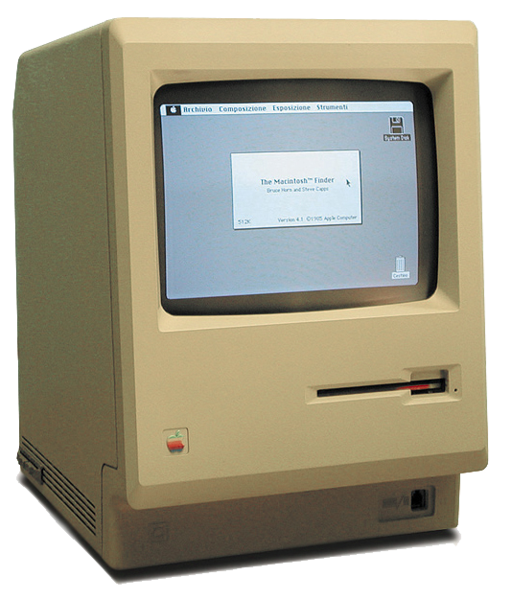
\includegraphics[width=0.5\textwidth]{./img/mac128.png}
\caption{\label{INTRO_mac128}Apple Macintosh (1984), popularizó la interfaz usuario gráfica (GUI). (Imagen de la Wikipedia: \emph{Macintosh})}
\end{figure}


Esto comenzó, sin embargo, a plantear inevitablemente las necesidades
de concurrencia a los programadores. Los programas ya no tenían acceso
directo a la pantalla para manipular a su antojo, sino que a una
abstracción (la \emph{ventana}) que podía variar sus medidas, y que
requería que toda la salida fuera estrictamente a través de llamadas a
bibliotecas de primitivas gráficas que comenzaron a verse como parte
integral del sistema operativo.

Además, los problemas de protección y separación entre procesos
concurrentes comenzaron a hacerse evidentes: los programadores tenían
ahora que programar con la conciencia de que compartirían recursos —
con el limitante (que no tenían en las máquinas \emph{profesionales}) de no
contar con hardware especializado para esta protección. Los
procesadores en uso comercial en los `80 no manejaban \emph{anillos} o
\emph{niveles de ejecución} ni \emph{unidad de administración de memoria} (MMU),
por lo que un programa fallado o dañino podía corromper la operación
completa del equipo. Y si bien los entornos que más éxito tuvieron
(Apple MacOS y Microsoft Windows) no implementaban multitarea real, sí
hubo desde el principio sistemas como la Commodore Amiga o la Atari ST
que hacían un multitasking \emph{preventivo} verdadero.

\begin{figure}[htb]
\centering
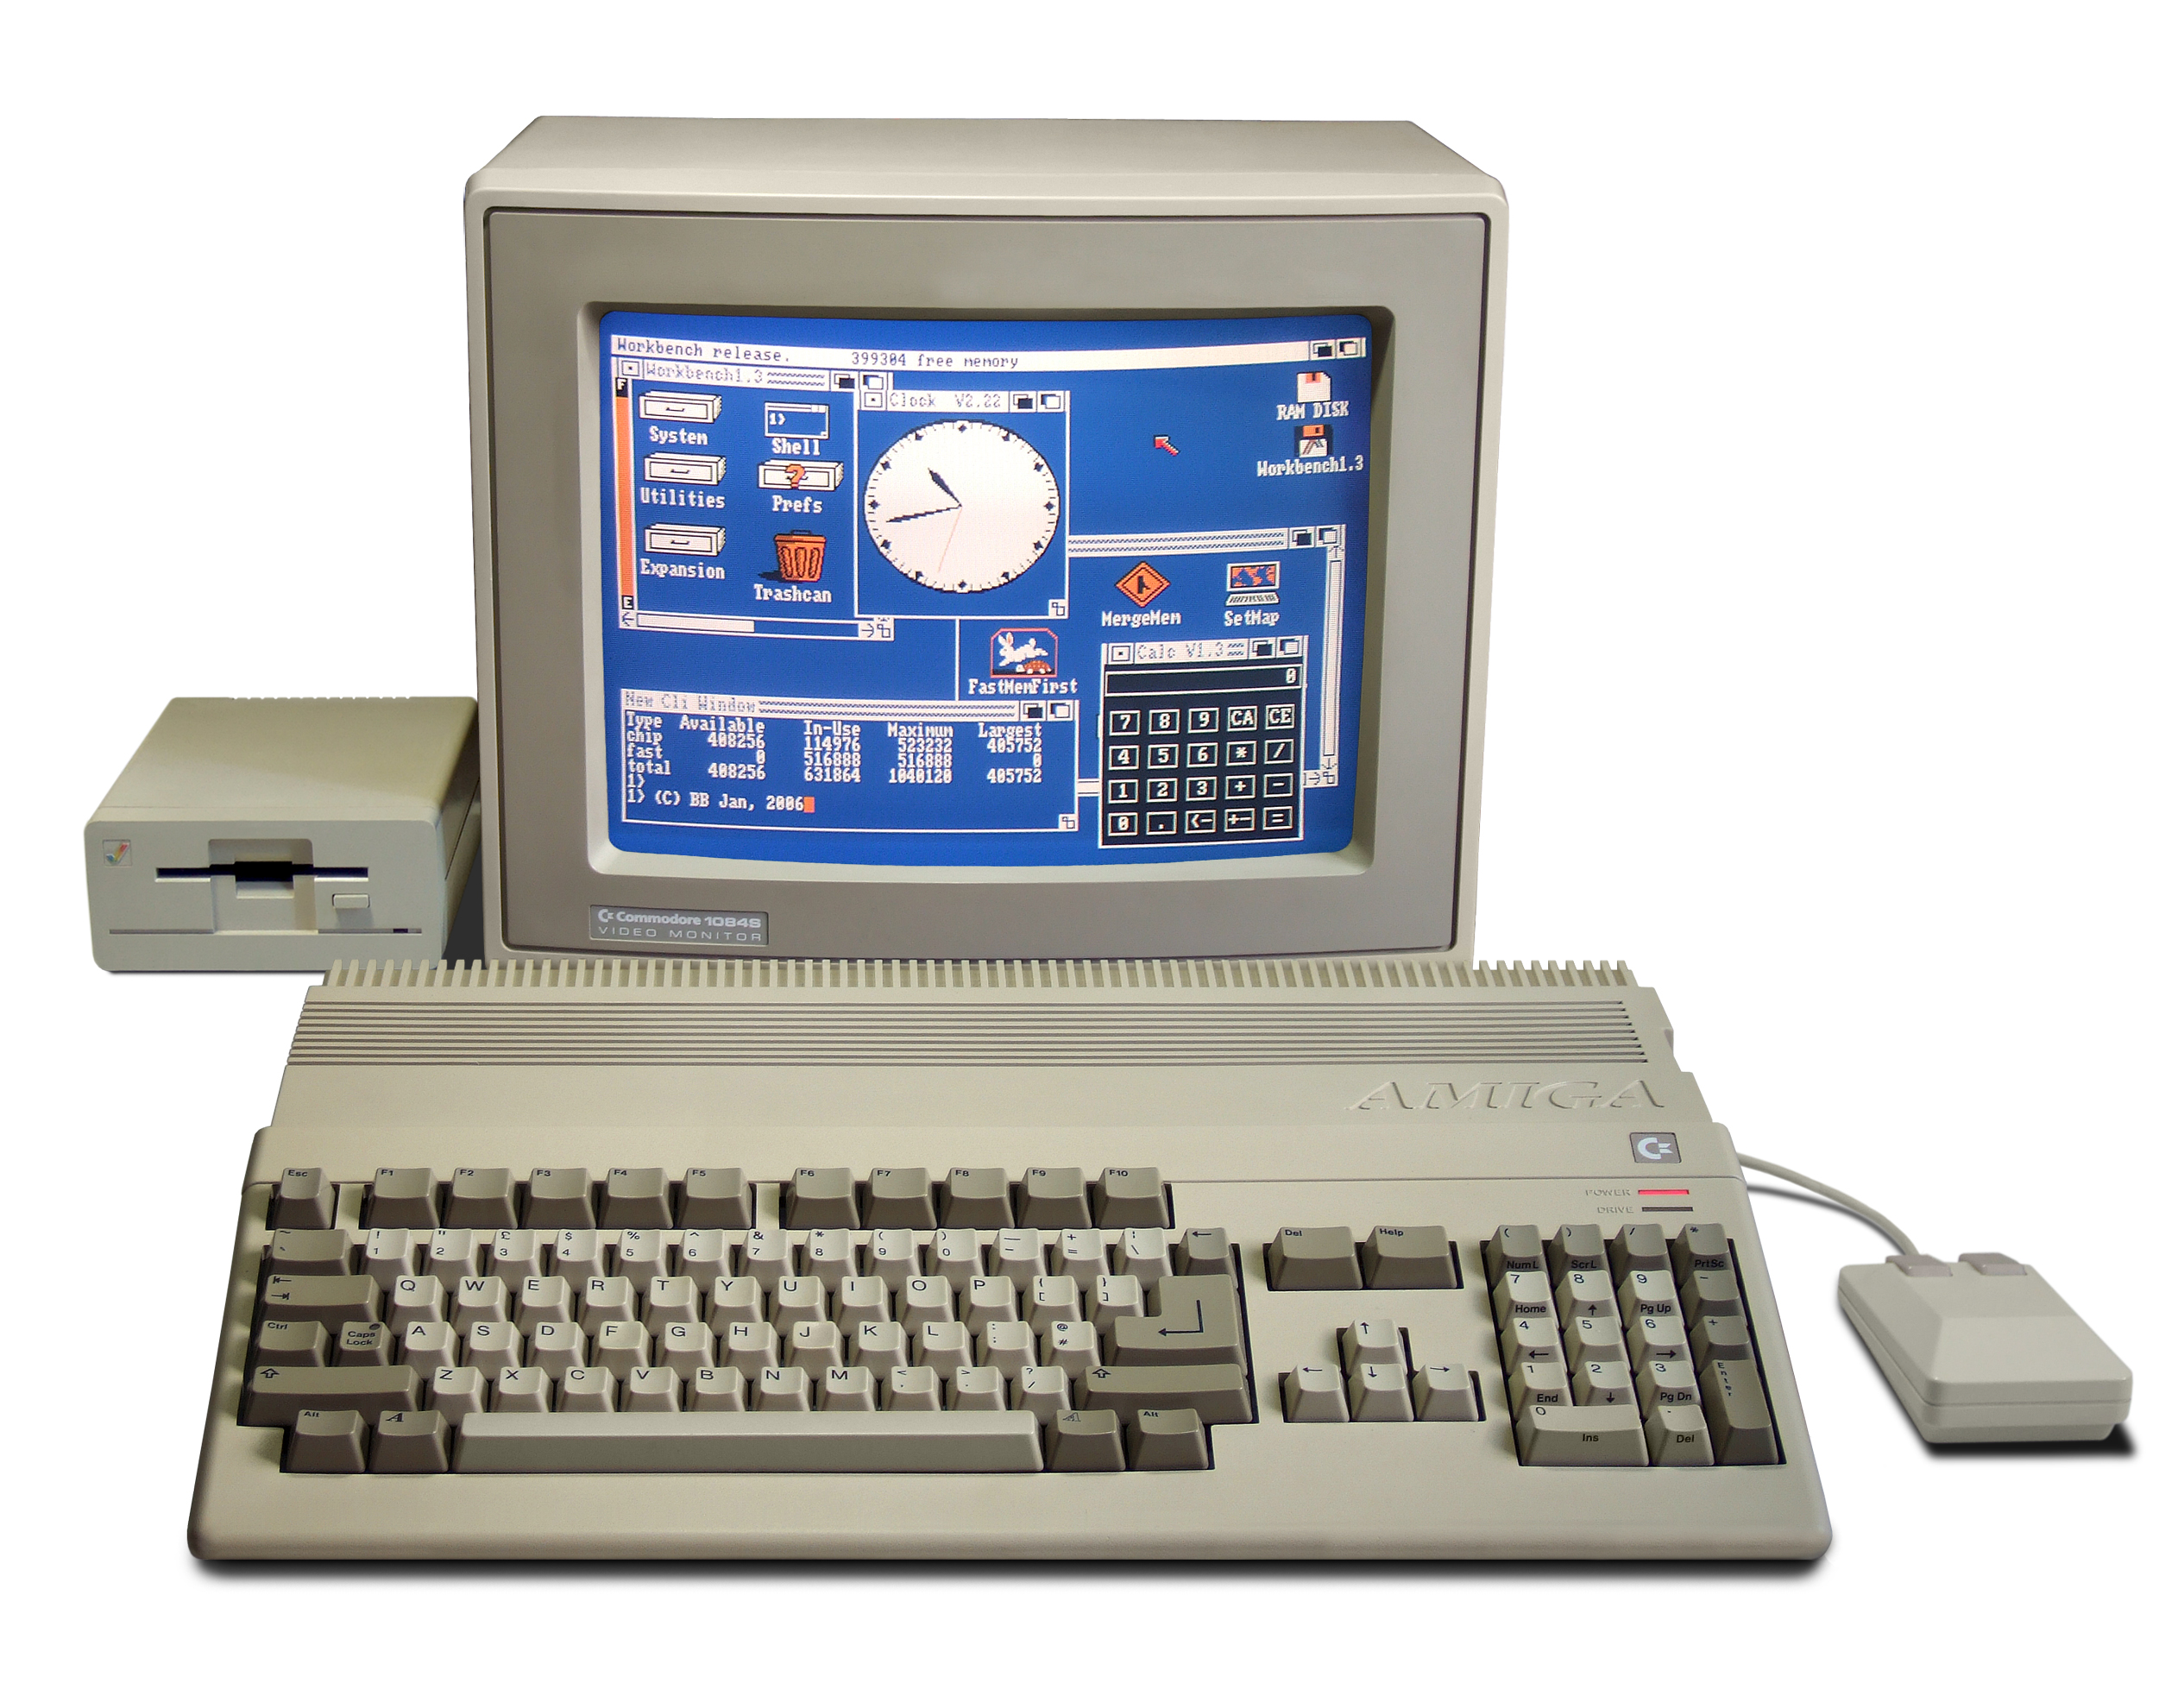
\includegraphics[width=0.5\textwidth]{./img/A500.jpg}
\caption{\label{INTRO_A1000}Commodore Amiga 500 (1987), la computadora más popular de la familia \emph{Amiga}, con amplias capacidades multimedia y multitarea preventiva; una verdadera maravilla para su momento. (Imagen de la Wikipedia: \emph{Amiga})}
\end{figure}

Naturalmente, ante el uso común de un entorno de ventanas, los
programas que se ejecutaban sin requerir de la carga del sistema
operativo cayeron lentamente en el olvido.
\subsection{Convergencia de los dos grandes mercados}
\label{sec-1-4-5}


Conforme fueron apareciendo los CPU con características suficientes
en el mercado para ofrecer la protección y aislamiento necesario
(particularmente, Intel 80386 y Motorola 68030), la brecha de
funcionalidad entre las computadoras personales y las \emph{estaciones de trabajo} y \emph{mainframes} se fue cerrando.

Hacia principios de los 1990, la mayor parte de las computadoras de
arquitecturas \emph{alternativas} fueron cediendo a las presiones del
mercado, y hacia mediados de la década sólo quedaban dos arquitecturas
principales: la derivada de IBM y la derivada de la Apple Macintosh.

Los sistemas operativos primarios para ambas plataformas fueron
respondiendo a las nuevas características del hardware: en las IBM, la
presencia de Microsoft Windows (originalmente un \emph{entorno operativo}
desde su primer edición en 1985, evolucionando hacia un sistema
operativo completo ejecutando sobre una base de MS-DOS en 1995) se fue
haciendo prevalente hasta ser la norma. Windows pasó de ser un sistema
meramente de aplicaciones propias y que operaba únicamente por reemplazo
de aplicación activa a ser un sistema de multitarea cooperativa, y
finalmente un sistema que requería protección en hardware (80386) e
implementaba multitarea preventiva.

A partir del 2003, el núcleo de Windows en más amplio uso fue
reemplazado por un desarrollo hecho de inicio como un sistema
operativo completo y ya no como una aplicación dependiente de MS-DOS:
el núcleo de Nueva Tecnología (Windows NT), que, sin romper
compatibilidad con los \emph{APIs} históricos de Windows, ofreció mucho
mayor estabilidad.

Por el lado de Apple, la evolución fue muy en paralelo: ante un
sistema ya agotado y obsoleto, el MacOS 9, en 2001 anunció una
nueva versión de su sistema operativo que fue en realidad un
relanzamiento completo: MacOS X es un sistema basado en un núcleo Unix
BSD, sobre el \emph{microkernel} Mach.

Y otro importante jugador que entró en escena durante los `90 fue el
software libre, por medio de varias implementaciones distintas de
sistemas tipo Unix — principalmente, Linux y los *BSD (FreeBSD,
NetBSD, OpenBSD). Estos sistemas implementaron, colaborativamente y a
escala mundial, software compatibles con las PC y con el que se ejecutaba en las
estaciones de trabajo a gran escala, con alta confiabilidad, y
cerrando por fin la divergencia del árbol del desarrollo de la
computación en \emph{fierros grandes} y \emph{fierros chicos}.

Al día de hoy, la arquitectura derivada de Intel (y la PC) es el claro
ganador de este proceso de 35 años, habiendo conquistado casi la
totalidad de los casos de uso, incluso las máquinas Apple.  
Hoy en día, la arquitectura Intel ejecuta
desde subportátiles hasta supercomputadoras y centros de datos; el
sistema operativo específico varía según el uso, yendo
mayoritariamente hacia Windows, con los diferentes Unixes concentrados
en los equipos servidores.

En el frente de los dispositivos \emph{embebidos} (las computadoras más
pequeñas, desde microcontroladores hasta teléfonos y tabletas), la
norma es la arquitectura ARM, también bajo versiones específicas de
sistemas operativos Unix y Windows (en ese orden).
\section{Organización de los sistemas operativos}
\label{sec-1-5}


Para comenzar el estudio de los sistemas operativos, la complejidad
del tema requiere que se haga de una forma modular. En este texto
no se busca enseñar cómo se usa un determinado sistema operativo, ni
siquiera comparar el uso de uno con otro (fuera de hacerlo con fines
de explicar diferentes implementaciones).

Al nivel que se estudiará, un sistema operativo es más bien un
gran programa, que ejecuta otros programas y les provee un
conjunto de interfaces para que puedan aprovechar los recursos de
cómputo. Hay dos formas primarias de organización \emph{interna} del
sistema operativo: los sistemas monolíticos y los sistemas
microkernel. Y si bien no se puede marcar una línea clara a rajatabla
que indique en qué clasificiación cae cada sistema, no es dificil
encontrar líneas bases.

\begin{description}
\item[Monolíticos] La mayor parte de los sistemas operativos
		 históricamente han sido \emph{monolíticos} — Esto
		 significa que hay un sólo \emph{proceso privilegiado} 
	  	 (justamente el sistema operativo) que
		 opera en modo supervisor, y dentro del cual se
		 encuentran todas las rutinas para las diversas tareas
		 que realiza el sistema operativo.

		 \begin{figure}[htb]
		 \centering
		 \includegraphics[width=0.7\textwidth]{./img/dot/diseno_monolitico.png}
		 \caption{\label{INTRO_diseno_monolitico}Esquematización de los componentes en un sistema monolítico}
		 \end{figure}
\item[Microkernel] El núcleo del sistema operativo se mantiene en el
                 mínimo posible de funcionalidad, descargando en
                 \emph{procesos especiales sin privilegios} las tareas que implementan el
                 acceso a dispositivos y las diversas políticas de uso
                 del sistema.

		 \begin{figure}[htb]
		 \centering
		 \includegraphics[width=0.7\textwidth]{./img/dot/diseno_microkernel.png}
		 \caption{\label{INTRO_microkernel}Esquematización de los componentes en un sistema microkernel}
		 \end{figure}
\end{description}

La principal ventaja de diseñar un sistema siguiendo un esquema
monolítico es la simplificación de una gran cantidad de mecanismos de
comunicación, que lleva a una mayor velocidad de ejecución (al
requerir menos cambios de contexto para cualquier operación
realizada). Además, al manejarse la comunicación directa como paso de
estructuras en memoria, el mayor acoplamiento permite más flexibilidad
al adecuarse para nuevos requisitos (al no tener que modificar no sólo
al núcleo y a los procesos especiales, sino también la interfaz
pública entre ellos).

Por otro lado, los sistemas microkernel siguen esquemas lógicos más
limpios, permiten implementaciones más elegantes y facilitan la
comprensión por separado de cada una de sus piezas. Pueden
\emph{auto-repararse} con mayor facilidad, dado que en caso de fallar uno
de los componentes (por más que parezca ser de muy bajo nivel), el
núcleo puede reiniciarlo o incluso reemplazarlo.

\begin{description}
\item[Sistemas con concepciones híbridas] No se puede  hablar de
     concepciones únicas ni de verdades absolutas. A lo largo del
     libro se verán ejemplos de \emph{concepciones híbridas} en este sentido
     — Sistemas que son mayormente monolíticos pero manejan algunos
     procesos que parecerían centrales a través de procesos de nivel
     usuario como los microkernel (por ejemplo, los sistemas de
     archivos en espacio de usuario, FUSE, en Linux).

     \begin{figure}[htb]
     \centering
     \includegraphics[width=0.7\textwidth]{./img/dot/diseno_hibrido.png}
     \caption{\label{INTRO_diseno_hibrido}Esquematización de los componentes en un sistema híbrido}
     \end{figure}
\end{description}
\section{Otros recursos}
\label{sec-1-6}


\begin{itemize}
\item \emph{On building systems that will fail}
  \otrorec{http://dl.acm.org/citation.cfm?id=1283947}
  Fernando J. Corbató
  (1990); ACM Turing award lectures
\item \emph{A Brief History of Computer Operating Systems}
  \otrorec{http://cs.gordon.edu/courses/cs322/lectures/history.html}
  R. Bjork (2000); Gordon College
\item \emph{Making EPERM friendlier}
  \otrorec{http://lwn.net/Articles/532771/}
  Michael Kerrisk (2013); Linux Weekly News: Explica algunas de las
  limitantes de la semántica POSIX: Falta de granularidad en el
  reporte de mensajes de error (\texttt{EPERM}), y \texttt{errno} global por hilo.
\item \emph{Biculturalism}
  \otrorec{http://www.joelonsoftware.com/articles/Biculturalism.html}
  Joel Spolsky (2003); Joel on Software
\end{itemize}
\chapter{Relación con el hardware}
\label{sec-2}
\section{Introducción}
\label{sec-2-1}
\label{HW}


Todos los sitemas de cómputo están compuestos por al menos una unidad de proceso
junto con dispositivos que permiten ingresar datos  (teclado, mouse, micrófono, 
etc.) y otros que permiten obtener resultados (pantalla, impresora, parlantes, 
etc.). Como se vio anteriormente, una de las funciones del sistema operativo es la de 
abstraer el hardware de la computadora y presentar al usuario una 
versión unificada y simplificada de los dispositivos.  
En este capítulo se verá la relación que mantiene el sistema operativo 
con el hardware, las funciones que cumplen y algunas abstracciones
comunes utilizadas en sistemas operativos modernos.
\section{Unidad de Procesamiento}
\label{sec-2-2}


La \emph{unidad de procesamiento} es la parte fundamental de todo sistema de cómputo.
Es la encargada de ejecutar tanto los programas del usuario como el sistema 
operativo en sí mismo.  La funciones del sistema operativo respecto a la
unidad de procesamiento son: 

\begin{description}
\item[Inicialización] Luego de ser cargado el sistema operativo debe realizar 
                    varias tareas de inicialización como habilitar 
                    las interrupciones de hardware y software 
                    (excepciones y trampas), configurar el sistema de 
                    memoria virtual (paginación, segmentación), etc.
\item[Atender las interrupciones y excepciones] Como se verá más adelante, 
                     la unidad de procesamiento 
                     puede encontrar una situación que no puede resolver
                     por sí misma (una instrucción o dirección inválida, 
                     una división por cero, etc.) ante lo cual le pasa el
                     control al sistema operativo para que éste trate o
                     resuelva la situación.
\item[Multiplexación] En un sistema multiproceso, el sistema operativo es el 
                    encargado de administrar la unidad de procesamiento 
                    dando la ilusión a los procesos que están ejecutando 
                    de forma exclusiva.
\end{description}
\subsection{Jerarquía de almacenamiento}
\label{sec-2-2-1}



Las computadoras que siguen la arquitectura \emph{von Neumann}, esto es,
prácticamente la totalidad hoy en día\footnote{Algunos argumentarán que
muchas de las computadoras en uso hoy en día siguen la arquitectura
\emph{Harvard modificada}, dado que empleando distintos bancos de memoria
caché, un procesador puede tanto referirse a la siguiente instrucción
como iniciar una transferencia de memoria primaria. Esta distinción no
tiene mayor relevancia para este tema, la referencia se incluye
únicamente por no llevar a confusión. } podrían resumir su operación
general a alimentar a una \emph{unidad de proceso} (CPU) con los datos e
instrucciones almacenados en \emph{memoria}, que pueden incluir llamadas a
servicio (y respuestas a eventos) originados en medios externos.

Una computadora von Neumann significa básicamente que es una
computadora de \emph{programa almacenado en la memoria primaria} — esto es,
se usa el mismo almacenamiento para el programa que está siendo
ejecutado y para sus datos, sirviéndose de un \emph{registro} especial para
indicar al CPU cuál es la dirección en memoria de la siguiente
instrucción a ejecutar.

La arquitectura von Neumann fue planteada, obviamente, sin considerar
la posterior diferencia entre la velocidad que adquiriría el CPU y la
memoria. En 1977, John Backus presentó al recibir el premio Turing un
artículo describiendo el \emph{cuello de botella de von Neumann}. Los
procesadores son cada vez más rápidos (se logró un aumento de 1000
veces tanto entre 1975 y 2000 tan sólo en el reloj del sistema), pero
la memoria aumentó su velocidad a un ritmo mucho menor —
aproximadamente un factor de 50 para la tecnología en un nivel
costo-beneficio suficiente para usarse como memoria primaria.

\begin{figure}[htb]
\centering
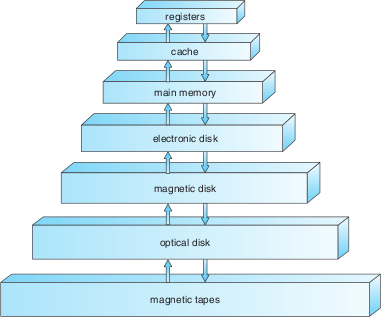
\includegraphics[height=0.5\textheight]{./img/dot/jerarquia_memoria.png}
\caption{\label{HW_jerarquia_memoria}Jerarquía de memoria entre diversos medios de almacenamiento.}
\end{figure}

Una respuesta parcial a este problema es la creación de una jerarquía
de almacenamiento, yendo de una pequeña área de memoria mucho más cara
hasta un gran espacio de memoria muy económica. En particular, la
relación entre las capas superiores está administrada por hardware
especializado de modo que su existencia resulta transparente al
programador.

\begin{table}[htb]
\caption{Velocidad y gestor de los principales niveles de memoria. (Silberschatz, Galvin, Gagne; p.28)} 
\begin{center}
\begin{tabular}{lllll}
 Nivel                   &  1                  &  2               &  3               &  4           \\
\hline
 \textbf{Nombre}         &  Registros          &  Cache           &  Memoria princ.  &  Disco       \\
 \textbf{Tamaño}         &  <1KB               &  <16MB           &  <64GB           &  >100GB      \\
 \textbf{Tecnología}     &  Multipuerto, CMOS  &  SRAM CMOS       &  CMOS DRAM       &  Magnética   \\
 \textbf{Acceso (ns)}    &  0.25-0.5           &  0.5-25          &  80-250          &  5,000,000   \\
 \textbf{Transf (MB/s)}  &  20,000-100,000     &  5,000-10,000    &  1,000-5,000     &  20-150      \\
 \textbf{Administra}     &  Compilador         &  Hardware        &  Sist. Op.       &  Sist. op.   \\
 \textbf{Respaldado en}  &  Cache              &  Memoria princ.  &  Disco           &  CD o cinta  \\
\end{tabular}
\end{center}
\end{table}


Ahora bien, si bien la relación entre estos medios de almacenamiento
puede parecer natural, para una computadora tiene una
realidad completamente distinta: los registros son parte integral del
procesador, y la memoria está a sólo un paso de distancia (el
procesador puede referirse a ella directamente, de forma transparente,
indicando la dirección desde un programa). El caché no existe para
efectos prácticos: el procesador no hace referencia directa a él, sino
que es manejado por los controladores de acceso a memoria.

Como se verá, el sistema operativo es el encargado de mantener todas estas 
jerarquías de memoria consistentes y de realizar las transferencias entre unas 
y otras.
\subsubsection{Registros}
\label{sec-2-2-1-1}


La memoria más rápida de la computadora son los \emph{registros}, ubicados
dentro de cada \emph{uno de los} núcleos de cada uno de los CPU. Las
arquitecturas tipo RISC (Reduced Instruction Set Computer) 
sólo contemplan la ejecución de instrucciones
entre registros (excepto, claro, las de carga y almacenamiento a
memoria primaria).

Los primeros CPU trabajaban con pocos registros, muchos de ellos de
propósito específico — trabajaban más bien con una lógica de \emph{registro acumulador}. Por ejemplo, el MOS 6502 (en el cual se basaron las
principales computadoras de 8 bits) tenía un acumulador de 8 bits (A),
dos registros índice de 8 bits (X e Y), un registro de estado del
procesador de 8 bits (P), un apuntador al \emph{stack} de 8 bits (S), y un
apuntador al programa de 16 bits (PC). El otro gran procesador de su
era, el Zilog Z80, tenía 14 registros (3 de 8 bits y el resto de 16),
pero sólo uno era un acumulador de propósito general.

El procesador Intel 8088, en el cual se basó la primer generación de
la arquitectura PC, ofrecía cuatro registros de uso \emph{casi} general. En
los ochenta comenzaron a producirse los primeros procesadores tipo RISC,
muchos de los cuales ofrecían 32 registros, todos ellos de propósito
general.

\begin{figure}[htb]
\centering
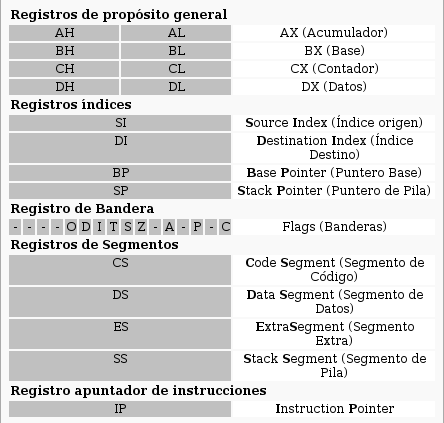
\includegraphics[width=0.6\textwidth]{./img/registros_8086.png}
\caption{\label{HW_registros_8086}Ejemplo de registros: Intel 8086/8088 (Imagen de la Wikipedia: \emph{Intel 8086 y 8088})}
\end{figure}

El compilador \footnote{A veces asistido por instrucciones explíticas por
parte del programador, pero muchas veces como resultado del análisis
del código. } busca realizar muchas operaciones que deben ocurrir
reiteradamente, donde la rapidez es fundamental, con sus operadores
cargados en los registros. El estado del CPU en un momento dado está
determinado por el contenido de los registros. El contenido de la
memoria, obviamente, debe estar sincronizado con lo que ocurre dentro
de éste — pero el estado actual del CPU, lo que está haciendo, las
indicaciones respecto a las operaciones recién realizadas que se deben
entregar al programa en ejecución están todos representados en los
registros. Se debe mantener esto en mente cuando posteriormente se
habla de todas las situaciones en que el flujo de ejecución debe ser
quitado de un proceso y entregado a otro.

La relación de la computadora y del sistema operativo con la memoria principal 
será abordada en el capítulo \ref{sec-5}.
\subsection{Interrupciones y excepciones}
\label{sec-2-2-2}
\label{HW_interrupciones}


La ejecución de los procesos podría seguir siempre linealmente,
atendiendo a las instrucciones de los programas tal como fueron escritas,
pero en el modelo de uso de cómputo actual, eso no serviría de
mucho: para que un proceso acepte interacción, su ejecución debe poder
responder a los \emph{eventos} que ocurran alrededor del sistema. Y los
eventos son manejados a través de las \emph{interrupciones} y \emph{excepciones}
(o \emph{trampas}).

Cuando ocurre algún evento que requiera la atención del sistema
operativo, el hardware encargado de procesarlo escribe directamente a
una ubicación predeterminada de memoria la naturaleza de la solicitud
(el \emph{vector de interrupción}) y, levantando una solicitud de
interrupción, \emph{detiene} el proceso que estaba siendo
ejecutado. El sistema operativo entonces ejecuta su \emph{rutina de manejo de interrupciones} (típicamente comienza grabando el estado de los
registros del CPU y otra información relativa al estado del proceso
desplazado) y posteriormente la atiende.

Las interrupciones pueden organizarse por \emph{prioridades}, de modo que
una interrupción de menor jerarquía no interrumpa a una más
importante — dado que las interrupciones muchas veces indican que hay
datos disponibles en algún buffer, el no atenderlas a tiempo podría
llevar a la pérdida de datos.

Hay un número limitado de interrupciones definidas para cada
arquitectura, mucho más limitado que el número de dispositivos que
tiene un equipo de cómputo actual. Las interrupciones son, por tanto,
generadas \emph{por el controlador del canal} en que son producidas. Si
bien esto resuelve la escasez de interrupciones, dificulta su
priorización — con canales de uso tan variado como el USB\footnote{Algunas
arquitecturas, particularmente de sistemas embebidos y por un criterio
altamente económico, están estructuradas íntegramente alrededor de un
bus USB. }, una interrupción puede indicar que hay desde un \emph{teclazo}
para ser leído hasta un paquete de red esperando a ser procesado — y
si bien demorar la atención al primero no llevaría a pérdida notable
de información, no ateneder el paquete de red sí.

El sistema operativo puede elegir ignorar (\emph{enmascarar}) a ciertas
interrupciones — pero hay interrupciones que son \emph{no enmascarables}.

Se hace la distinción entre interrupciones y excepciones según su
origen: una interrupción es generada por causas externas al sistema
(un dispositivo requiere atención), mientras que una excepción es una
evento generado por un proceso (una condición en el proceso que
requiere la intervención del sistema operativo). Si bien hay
distinciones sutiles entre interrupciones, trampas y excepciones, al
nivel de discusión que se abordará basta con esta distinción.

Los eventos pueden ser, como ya se mencionó, indicadores de que hay algún
dispositivo requiriendo atención, pero pueden también provenir del
mismo sistema, como una \emph{alarma} o \emph{temporizador} (que se emplea para
obligar a todo programa a entregar el control en un sistema
multitareas) o indicando una condición de error (por ejemplo, una
división sobre cero o un error leyendo de disco).

Las funciones del sistema operativo respecto a las interrupciones son:

\begin{description}
\item[Administrar el hardware manejador de interrupciones] Esto incluye el enmascarado y desenmascarado 
                                  de las interrupciones, configurar y asignar
                                  interrupciones a cada dispositivo, 
                                  notificar al manejador cuando la interrupción
                                  ya ha sido atendida, etc.
\item[Abstraer las interrupciones] El sistema operativo oculta a los programas de
                                  usuario la existencia de interrupciones de
                                  hardware ya que éstas son dependientes de la
                                  arquitectura del procesador. En cambio el
                                  sistema operativo lo comunica de una forma
                                  unificada a través de distintos mecanismos,
                                  por ejemplo mensajes o señales o detiendo el
                                  proceso que espera la acción relacionada con
                                  una interrupción y continuando su ejecución
                                  cuando ésta ocurre.
\item[Punto de entrada al sistema operativo] Como se verá más adelante en la 
                                sección \ref{HW_SYSCALLS}, muchos procesadores y
                                sistemas operativos utilizan las interrupciones
                                como medio por el cual un proceso de usuario
                                realiza una llamada al sistema.
                                Por ejemplo, en Linux para arquitecturas x86
                                el programa de usuario genera la interrupción
                                0x80 para iniciar una llamada al sistema.
                                En arquitecturas más recientes como x86$_{\mathrm{64}}$,
                                MIPS y ARM esto ha sido reemplazado por una
                                instrucción especial \texttt{syscall}.
\item[Atender excepciones y fallas] Como se discutió antes, durante la
     ejecución de un programa pueden ocurrir situaciones anómalas, 
     como por ejemplo, una división sobre cero. Desde el punto de
     vista del CPU, esto es similar a una interrupción de hardware y
     debe ser tratada por el sistema operativo. Dependiendo de la
     causa de la excepción, el sistema operativo tomará acción para
     resolver en lo posible esta situación. En muchos casos las
     excepciones resultan en una señal enviada al proceso, y este
     último es el encargado de tratar la excepción. En otros casos la
     falla o excepción son irrecuperables (una instrucción inválida o
     un error de bus) ante la cual el sistema operativo terminará el
     proceso que la generó.  En el capítulo \ref{sec-5} se cubre con mucho
     mayor detalle un tipo de excepción muy importante que debe tratar
     el sistema operativo: el fallo de paginación.
\end{description}
\section{Terminales}
\label{sec-2-3}

Las terminales son dispositivos electrónicos utilizados para ingresar datos
y emitir resultados dentro de un sistema de cómputo. 
Las primeras terminales utilizaban tarjetas
perforadas e impresiones en papel. Debido a su limitada velocidad e
imposibilidad de ``editar'' el papel ya impreso, este tipo de terminales
fue cediendo terreno ante la aparición sobre principios de los setenta 
de las terminales de texto con pantalla de video y teclado.

Conceptualmente una terminal de texto es un dispositivo mediante el cual
la computadora recibe y envía un flujo de caracteres desde y hacia el usuario respectivamente.
Las operaciones más complejas, como edición, borrado y movimiento,
en general son tratadas con \emph{secuencias de escape}, esto es, una serie
de caracteres simples que tomados en conjunto representan una acción
a realizar en la terminal. 

Durante la década de los setenta también se desarrollaron terminales 
gráficas las cuales podían representar imágenes junto 
con texto. Con la inclusión del ratón o ``mouse''
estas terminales dieron lugar a lo que hoy se conoce
como Interfaz Gráfica de Usuario (\emph{Graphical User Interface} o \emph{GUI})
y a los sistemas de ventana.

En los sistemas operativos modernos es común referirse al \emph{emulador de terminal}, un programa especializado ya sea para tener múltiples
instancias de una terminal o para ejectuar una terminal de texto dentro de una
interfaz gráfica. Estos programas se denominan de esta forma dado que
sólo replican el comportamiento de las terminales (que eran
originalmente equipos independientes), siendo únicamente un programa
que recibe la entrada del usuario a través del teclado enviándola al
sistema operativo como un flujo de datos, y recibe otro flujo de datos
del sistema operativo, presentándolo de forma adecuada al
usuario.
\section{Dispositivos de almacenamiento}
\label{sec-2-4}


El almacenamiento en memoria primaria es \emph{volátil}, esto es, se pierde
al interrumpirse el suministro eléctrico. Esto no era muy importante
en la época definitoria de los conceptos que se presentan en esta sección,
dado que el tiempo total de vida de un conjunto de datos en
almacenamiento bajo el control del procesador iba únicamente desde la
entrada y hasta el fin de la ejecución del trabajo del usuario. Pero
desde la década de los sesenta se popularizó la posibilidad de
almacenar en la computadora información \emph{a largo plazo} y con
expectativas razonables de permanencia.

De las muchas tecnologías de almacenamiento, la que ha dominado
fuertemente durante los últimos 40 años ha sido la de los discos
magnéticos\footnote{Se verán en la sección \ref{FS_FIS_estado_solido} detalles
acerca de las tecnologías de almacenamiento \emph{en estado sólido}, que
pueden poner fin a esta larga dominación. }. El acceso a disco (miles
de veces más lento que el acceso a memoria) no es realizado
directamente por el procesador, sino que requiere de la comunicación
con controladores externos, con lógica propia, que podrían ser vistos
como computadoras independientes de propósito limitado.

El procesador no puede referirse directamente más información que la
que forma parte del almacenamiento primario — esto es, de la memoria
RAM. En las secciones \ref{HW_interrupciones}
(\emph{Interrupciones y excepciones}) y \ref{HW_dma} (\emph{Acceso directo a memoria}), se explica cómo es que se efectúan dichas referencias.

Los dispositivos de almacenamiento (discos, memorias flash, cintas)
pueden ser vistos como una región donde la computadora lee y escribe
una serie de bytes que preservarán su valor incluso luego de apagada
la computadora.

A nivel de hardware el sistema operativo no accede al dispositivo de
almacenamiento byte por byte, sino que éstos se agrupan en \emph{bloques}
de tamaño fijo.  El manejo de estos bloques (adminstración de bloques
libres, lectura y escritura) es una tarea fundamental del sistema
operativo, que asimismo se encarga de presentar abstracciones como la
de archivos y directorios al usuario. Esto se verá en el capítulo
\ref{sec-6}.
\section{Relojes y temporizadores}
\label{sec-2-5}

Todas las computadoras incluyen uno o más relojes y 
temporizadores que son utilizados para funciones varias como 
mantener la hora del sistema actualizada, implementar alarmas tanto para los
programas de usuario como para el sistema operativo, ejecutar
tareas de mantenimiento periódicas, cumplir con requisitos
temporales de aplicaciones de tiempo real, etc.

Mantener el tiempo correctamente dentro del sistema operativo
es algo crucial. Permite establecer un orden cronológico 
entre los eventos que ocurren dentro del sistema, por ejemplo
la creación de un archivo y de otro o el tiempo consumido
en la ejecución de un proceso. 

Por otro lado si el sistema operativo utiliza una política de 
planificación de procesos preventiva (capítulo \ref{sec-4}), 
como la \emph{Ronda} (\emph{Round Robin}),  éste debe interrumpir al proceso
en ejecución luego de cierta cantidad de unidades de tiempo. Esto
se implementa haciendo que el temporizador de la computadora
genere interrupciones periódicamente, lo cual luego invocará al planificador
de procesos.
\section{Canales y puentes}
\label{sec-2-6}


Los distintos componentes de un sistema de cómputo se comunican a
través de los diferentes \emph{canales} (generalmente se hace referencia a
ellos por su nombre en inglés: \emph{buses}). Al nivel más
básico, los canales son líneas de comunicación entre el procesador
y los demás componentes del chipset\footnote{Los chips que forman parte de
un equipo, casi siempre provistos por el mismo fabricante que el
procesador mismo. }, a los cuales a su vez se conectan los diferentes
dispositivos del sistema — desde aquellos que requieren mayor
velocidad, como la misma memoria, hasta los puertos más sencillos.

Un chipset provee distintos buses, con un agrupamiento lógico
según la velocidad requerida por sus componentes y otras
características que determinan su topología.

\begin{figure}[htb]
\centering
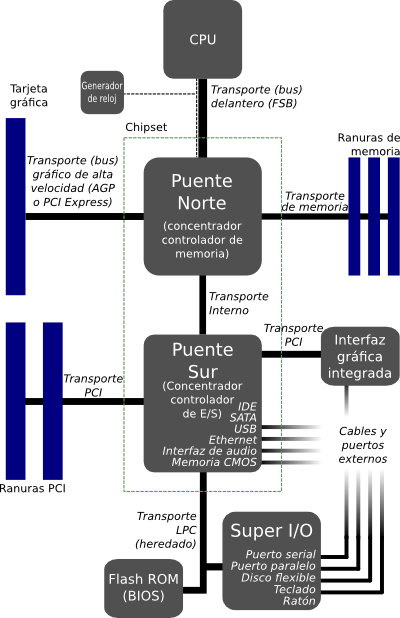
\includegraphics[width=0.5\textwidth]{./img/northbridge_southbridge.png}
\caption{\label{HW_northbridge_southbridge}Diagrama de la comunicación entre componentes de un sistema de cómputo basado en \emph{puente norte} y \emph{puente sur}}
\end{figure}

Hoy en día, el acomodo más frecuente\footnote{La separación aquí descrita
ha sido característica de las computadoras x86 de los últimos 20 años,
aunque la tendencia apunta a que se abandone paulatinamente para dar
paso a procesadores que integren en un sólo paquete todos estos
componentes. Sin embargo, el acomodo funcional electrónico, al menos
hasta el momento, sigue basado en estos puntos. } de estos buses es a
través de una separación en dos chips: el \emph{puente norte}
(\emph{Northbridge}), conectado directamente al CPU, encargado de gestionar
los buses de más alta velocidad y que, además, son fundamentales para
el más básico inicio de la operación del sistema: la memoria y el
reloj. La comunicación con algunas tarjetas de video se incorpora al
puente norte a través del canal dedicado \emph{AGP} (\emph{Advanced Graphics Port}, \emph{Puerto Gráfico Avanzado}).

Al puente norte se conecta el \emph{puente sur} (\emph{Southbridge}), que
controla el resto de los dispositivos del sistema — normalmente
se ven aquí las interfaces de almacenamiento (SCSI, SATA, IDE), de
expansión interna (PCI, PCIe) y de expansión externa (USB, Firewire,
puertos \emph{heredados} seriales y paralelos).
\subsection{Contención}
\label{sec-2-6-1}


Una de las principales razones de la existencia de tantos \emph{canales}
(buses) distintos en un mismo sistema es a la frecuencia acorde a los
dispositivos para los cuales está diseñado: la cantidad de datos que
tiene que viajar entre el procesador y la memoria a lo largo de la
operación del sistema es muy superior que la que tiene que
transferirse desde los discos, y a su vez, esta es mucho mayor que la
que enviarse a la impresora, o la que se recibe del teclado. Claro
está, los demás dispositivos podrían incrementar su frecuencia para
participar en un canal más rápido, aunque su costo se incrementaría,
dado que harían falta componentes capaces de sostener un reloj varios
órdenes de magnitud más rápido.

Pero incluso obviando la diferencia económica: cuando el sistema
requiere transferir datos de o hacia varios dispositivos de la misma
categoría, es frecuente que ocurra \emph{contención}: puede saturarse el
ancho de banda máximo que alcanza uno de los canales y, aún si los
dispositivos tienen información lista, tendrán que esperar a que los
demás dispositivos desocupen el canal.

\begin{figure}[htb]
\centering
\includegraphics[width=\textwidth]{./img/dot/chipset_857.png}
\caption{\label{HW_chipset_857}Esquema simplificado del chipset Intel 875 (para el procesador Pentium 4) ilustrando la velocidad de cada uno de los canales}
\end{figure}

En la figura \ref{HW_chipset_857} se puede ver el diseño general del
chipset Intel 875, introducido en el 2003, incluyendo el ancho de
banda de cada uno de los canales del sistema. Hay que recordar que hay
canales como el USB que permiten la conexión de múltiples
dispositivos, los cuales deberán compartir el ancho de banda total
permitido por el canal: en la figura se presentan dos discos duros
sobre el canal SATA y dos unidades ópticas en el ATA paralelo; el
canal USB permite el uso de un máximo de 127 unidades por canal, por
lo cual la contención puede ser muy alta.
\subsection{Acceso directo a memoria (DMA)}
\label{sec-2-6-2}
\label{HW_dma}


La operación de dispositivos de entrada/salida puede ser altamente
ineficiente. Cuando un proceso está en una sección \emph{limitada por entrada-salida} (esto es, donde la actividad principal es la
transferencia de información entre la memoria principal y cualquier
otra área del sistema), si el procesador tiene que encargarse de la
transferencia de toda la información\footnote{Este modo de operación es
también conocido como \emph{entrada/salida programada}. }, se crearía un
cuello de botella por la cantidad y frecuencia de interrupciones. Hoy
en día, para evitar que el sistema se demore cada vez que hay una
transferencia grande de datos, todas las computadoras implementan
controladores de \emph{acceso directo a memoria} (DMA) en uno o más de sus
subsistemas.

El DMA se emplea principalmente al tratar con dispositivos con un
gran ancho de banda, como unidades de disco, subsistemas multimedia,
tarjetas de red, e incluso para transferir información entre niveles
del caché.

Las transferencias DMA se hacen en \emph{bloques} preestablecidos; en vez
de que el procesador reciba una interrupción cada vez que hay una palabra
lista para ser almacenada en la memoria, el procesador indica al
controlador DMA la dirección física base de memoria en la cual
operará, la cantidad de datos a transferir, el \emph{sentido} en que se
efectuará la operación (del dispositivo a memoria o de memoria al
dispositivo), y el \emph{puerto} del dispositivo en cuestión; el
controlador DMA efectuará la transferencia solicitada, y sólo una vez
terminada ésta (o en caso de encontrar algún error en el proceso)
lanzará una interrupción al sistema; el procesador queda libre para
realizar otras tareas, sin más limitante que la posible \emph{contención}
que tendrá que enfrentar en el bus de acceso a la memoria.
\subsubsection{Coherencia de cache}
\label{sec-2-6-2-1}


Cuando se realiza una transferencia DMA de un dispositivo a la
memoria, puede haber \emph{páginas} de la memoria en cuestión que estén en
alguno de los niveles de la memoria caché; dado que el caché está uno
o más niveles por encima de la memoria principal, es posible que la
información haya ya cambiado pero el caché retenga la información
anterior.

Los sistemas de \emph{caché coherente} implementan mecanismos en hardware
que notifican a los controladores de caché que las páginas que alojan
están \emph{sucias} y deben ser vueltas a cargar para ser empleadas, los
sistemas \emph{no coherentes} requieren que el subsistema de memoria del
sistema operativo haga esta operación.

Los procesadores actuales implementan normalmente varios niveles de
caché, estando algunos dentro del mismo CPU, por lo que típicamente
se encuentran sistemas híbridos, en los que los cachés de nivel 2 son
coherentes, pero los de nivel 1 no, y deben ser manejados por
software.
\section{Interfaz del Sistema Operativo: llamadas al sistema}
\label{sec-2-7}
\label{HW_SYSCALLS}

De forma análoga a las interrupciones, se puede hablar
de las llamadas al sistema. El sistema operativo protege a un proceso
de otro, y previene que un proceso ejecutándose en espacio no
privilegiado tenga acceso directo a los dispositivos. Cuando un
proceso requiere de alguna acción privilegiada, acede a ellas realizando 
una \emph{llamada al sistema}. Las llamadas al sistema pueden agruparse, a
grandes rasgos, en:

\begin{description}
\item[Control de procesos] Crear o finalizar un proceso, obtener
     atributos del proceso, esperar la finalización de un proceso o cierto tiempo, 
	asignar o liberar memoria, etc.
\item[Manipulación de archivos] Crear, borrar o renombrar un archivo;
     abrir o cerrar un archivo existente; modificar sus \emph{metadatos};
     leer o escribir de un \emph{descriptor de archivo} abierto, etc.
\item[Manipulación de dispositivos] Solicitar o liberar un dispositivo;
     leer, escribir o reposicionarlo, y otras varias. Muchas de estas
     llamadas son análogas a las de manipulación de archivos, y varios
     sistemas operativos las ofrecen como una sola.
\item[Mantenimiento de la información] Obtener o modificar la hora del
     sistema; pedir detalles acerca de procesos o archivos, etc.
\item[Comunicaciones] Establecer una comunicación con determinado
                    proceso (local o remoto), aceptar una solicitud de
                    comunicación de otro proceso, intercambiar
                    información sobre un canal establecido.
\item[Protección] Consultar o modificar la información relativa al
                acceso de objetos en el disco, otros procesos, o la
                misma sesión de usuario.
\end{description}

Cada sistema operativo \emph{expone} una serie de llamadas al
sistema. Estas son, a su vez, expuestas al programador a través de las
\emph{interfaces de aplicación al programador} (API), que se alínean de
forma cercana (pero no exacta). Del mismo modo que cada sistema
operativo ofrece un conjunto de llamadas al sistema distinto, cada
implementación de un lenguaje de programación puede ofrecer un API
ligeramente distinto de otros.

\begin{figure}[htb]
\centering
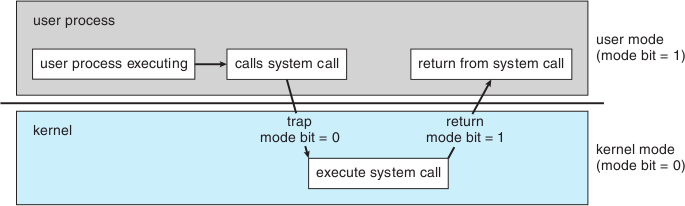
\includegraphics[width=\textwidth]{./img/dot/llamada_al_sistema.png}
\caption{\label{HW_llamada_al_sistema}Transición del flujo entre espacio usuario y espacio núcleo en una llamada al sistema}
\end{figure}
\subsection{Llamadas al sistema, arquitecturas y APIs}
\label{sec-2-7-1}
\label{HW_syscall_arch_api}


Cada familia de sistemas operativos provee distintas llamadas al sistema, y
sus lenguajes/bibliotecas implementan distintos APIs. Esto es el que
distingue principalmente a uno de otro. Por ejemplo, los sistemas
Windows 95 en adelante implementan Win32, Win16 (compatibilidad con
Windows previos) y MSDOS; MacOS implementa Cocoa (aplicaciones MacOS
X) y Carbon (compatibilidad con aplicaciones de MacOS previos), y
Linux y los *BSDs, POSIX (el estándar que define a Unix). El caso de
MacOS X es interesante, porque también implementa POSIX, ofreciendo la
\emph{semántica} de dos sistemas muy distintos entre sí.

Los lenguajes basados en \emph{máquinas virtuales abstractas}, como Java o
la familia .NET, exponen un API con mucha mayor distancia respecto al
sistema operativo; la máquina virtual se presenta como un
pseudo-sistema operativo intermedio que se ejecuta dentro del real, y
esta distinción se hace especialmente notoria cuando se busca conocer
los detalles del sistema operativo. 
\subsubsection{Depuración por \emph{trazas} (trace)}
\label{sec-2-7-1-1}


La mayor parte de los sistemas operativos ofrecen programas que, para
fines de depuración, \emph{envuelven} al API del sistema y permiten ver la
\emph{traza} de las llamadas al sistema que va realizando un
proceso. Algunos ejemplos de estas herramientas son \texttt{strace} en Linux,
\texttt{truss} en la mayor parte de los Unixes históricos o \texttt{ktrace} y
\texttt{kdump} en los *BSD. A partir de Solaris 10 (2005), Sun incluye una
herramienta mucho más profunda y programable para esta tarea llamada
\texttt{dtrace}, que al paso del tiempo ha sido \emph{portada}\footnote{Se denomina
\emph{portar} el hacer las adecuaciones necesarias para que una herramienta
diseñada para determinado entorno pueda emplearse en otros distintos. }
a otros Unixes (*BSD, MacOS).

La salida de una traza brinda amplio detalle acerca de la
actividad realizada por un proceso, y permite comprender a grandes
rasgos su interacción con el sistema. El nivel de información que da
es, sin embargo, a veces demasiado — eso se puede ver si se considera
la siguiente traza, ante uno de los comandos más sencillos: \texttt{pwd}
(obtener el directorio actual)

{\scriptsize

\begin{verbatim}
$ strace pwd
execve("/bin/pwd", ["pwd"], [/* 43 vars */]) = 0
brk(0)                                  = 0x8414000
access("/etc/ld.so.nohwcap", F_OK)      = -1 ENOENT (No such file or directory)
mmap2(NULL, 8192, PROT_READ|PROT_WRITE, MAP_PRIVATE|MAP_ANONYMOUS, -1, 0) = 0xb773d000
access("/etc/ld.so.preload", R_OK)      = -1 ENOENT (No such file or directory)
open("/etc/ld.so.cache", O_RDONLY)      = 3
fstat64(3, {st_mode=S_IFREG|0644, st_size=78233, ...}) = 0
mmap2(NULL, 78233, PROT_READ, MAP_PRIVATE, 3, 0) = 0xb7729000
close(3)                                = 0
access("/etc/ld.so.nohwcap", F_OK)      = -1 ENOENT (No such file or directory)
open("/lib/i386-linux-gnu/libc.so.6", O_RDONLY) = 3
read(3, "\177ELF\1\1\1\0\0\0\0\0\0\0\0\0\3\0\3\0\1\0\0\0po\1\0004\0\0\0"..., 512) = 512
fstat64(3, {st_mode=S_IFREG|0755, st_size=1351816, ...}) = 0
mmap2(NULL, 1366328, PROT_READ|PROT_EXEC, MAP_PRIVATE|MAP_DENYWRITE, 3, 0) = 0xb75db000
mprotect(0xb7722000, 4096, PROT_NONE)   = 0
mmap2(0xb7723000, 12288, PROT_READ|PROT_WRITE, MAP_PRIVATE|MAP_FIXED|MAP_DENYWRITE, 3, 0x147) = 0xb7723000
mmap2(0xb7726000, 10552, PROT_READ|PROT_WRITE, MAP_PRIVATE|MAP_FIXED|MAP_ANONYMOUS, -1, 0) = 0xb7726000
close(3)                                = 0
mmap2(NULL, 4096, PROT_READ|PROT_WRITE, MAP_PRIVATE|MAP_ANONYMOUS, -1, 0) = 0xb75da000
set_thread_area({entry_number:-1 -> 6, base_addr:0xb75da8d0, limit:1048575, seg_32bit:1, contents:0, read_exec_only:0, limit_in_pages:1, seg_not_present:0, useable:1}) = 0
mprotect(0xb7723000, 8192, PROT_READ)   = 0
mprotect(0xb775c000, 4096, PROT_READ)   = 0
munmap(0xb7729000, 78233)               = 0
brk(0)                                  = 0x8414000
brk(0x8435000)                          = 0x8435000
open("/usr/lib/locale/locale-archive", O_RDONLY|O_LARGEFILE) = 3
fstat64(3, {st_mode=S_IFREG|0644, st_size=1534672, ...}) = 0
mmap2(NULL, 1534672, PROT_READ, MAP_PRIVATE, 3, 0) = 0xb7463000
close(3)                                = 0
getcwd("/home/gwolf/vcs/sistemas_operativos", 4096) = 36
fstat64(1, {st_mode=S_IFCHR|0620, st_rdev=makedev(136, 1), ...}) = 0
mmap2(NULL, 4096, PROT_READ|PROT_WRITE, MAP_PRIVATE|MAP_ANONYMOUS, -1, 0) = 0xb773c000
write(1, "/home/gwolf/vcs/sistemas_operati"..., 36/home/gwolf/vcs/sistemas_operativos
) = 36
close(1)                                = 0
munmap(0xb773c000, 4096)                = 0
close(2)                                = 0
exit_group(0)                           = ?
\end{verbatim}
}
\section{Abstracciones comunes}
\label{sec-2-8}
\label{HW_abstracciones}


Como se mencionó antes una de las funciones del sistema operativo es
la de abstraer el hardware de la computador. Cuál es esa abstracción
que ve efectivamente el usuario varía de un sistema operativo a otro.
Se verán en esta sección algunas abstracciones utilizadas en varios
sistemas dejando las correspondientes a sistemas de archivos para el 
capítulo \ref{sec-7}.
\subsection{Sistemas tipo Windows}
\label{sec-2-8-1}

Los sistemas del tipo Windows presentan una abstracción diversa
para cada uno de los componentes de la computadora.

Por ejemplo los volúmenes de almacentamiento secundario (discos rígidos, 
discos compactos, memorias flash, etc.) son relacionados 
con una letra cada uno, así (en general) \texttt{C:} es el volumen o partición
del disco principal, \texttt{A:} y \texttt{B:} se utilizan para discos
extraibles.

Una desventaja de esta abstracción es que no queda claro cuáles unidades
pertenecen al mismo disco físico y cuáles no.

A los puertos de entrada/salida más utilizados también se les asignan
nombres alfanuméricos, por ejemplo el primer puerto paralelo se denomina
\texttt{LPT1} y el segundo puerto serie \texttt{COM2}. 
\subsection{Sistemas tipo Unix}
\label{sec-2-8-2}
\label{HW_sist_unix}


Unix introdujo el concepto de que \emph{todo es un archivo}: en el sistema
Unix original, todos los dispositivos podían ser controlados a través
de un \emph{archivo especial} que, en vez de almacenar información, apunta
a estructuras en el sistema que controlan a cada dispositivo. Este
concepto sobrevive en los sistemas derivados de Unix al día de hoy,
aunque varias clases de dispositivo rompen esta lógica. El sistema
operativo \emph{Plan9} de Bell Labs mantiene y amplía este concepto e
introduce los \emph{espacios de nombres mutables}, que presenta con
interfaz de archivo prácticamente cualquier objeto empleado
por el sistema.

Las principales estructuras relacionadas de este tipo que existen en un
sistema tipo Unix son:

\begin{description}
\item[Dispositivos de caracteres] Son aquellos en los cuales la
     información es leída o escrita de a un caracter a la vez y se
     presentan como \emph{streams} (flujos) de información, ya sea
     entrante, saliente o mixta. Algunos pueden permitir operaciones
     adicionales (por ejemplo, rebobinado), pero la manipulación de la
     información se efectúa de forma secuencial.

     Ejemplos: impresora, unidad de cinta, modem.
\item[Dispositivos de bloques] Presentan una interfaz
     de \emph{acceso aleatorio} y entregan o reciben la información en
     \emph{bloques} de tamaño predeterminado.

     El ejemplo más claro de este tipo de dispositivos es una unidad
     de disco o una de sus particiones.
\item[Archivos especiales] Los sistemas Unix actuales incluyen también
  un gran número de archivos especiales, por medio de los cuales el usuario puede
  monitorear el estado del sistema (memoria libre, número de procesos,
  consumo de procesador, etc.), e incluso modificar la configuración
  del sistema operativo a través de un archivo; por ejemplo, en un sistema Linux,
  escribir el valor ``100'' al archivo ``/proc/sys/vm/swappiness'' hará
  que el sistema envíe a espacio de intercambio una mayor cantidad de
  programas de lo que normalmente haría.
\end{description}
\section{Cuando dos cabezas piensan mejor que una}
\label{sec-2-9}
\subsection{Multiprocesamiento}
\label{sec-2-9-1}


El \emph{multiprocesamiento} es todo entorno donde hay más de un procesador
(CPU). En un entorno multiprocesado, el conjunto de procesadores se
vuelve un recurso más a gestionar por el sistema operativo — y el que
haya concurrencia \emph{real} tiene un fuerte impacto en su diseño.

Si bien en el día a día se usan de forma intercambiable\footnote{O poco
más que eso, al grado de que rara vez se emplea el término
\emph{multiprogramación}, mucho más acorde a los equipos que se emplean día
a día. }, es importante enfatizar en la diferencia fundamental entre el
\emph{multiprocesamiento}, que se abordará en esta sección, y la
\emph{multiprogramación}, de la cual se hablará en la sección
\ref{INTRO_multiprogramados} (\emph{Sistemas multiprogramados}). Un sistema
multiprogramado da la \emph{ilusión} de que está ejecutando varios
procesos al mismo tiempo, pero en realidad está alternando entre los
diversos procesos que compiten por su atención. Un sistema
multiprocesador tiene la capacidad de estar atendiendo
\emph{simultáneamente} a diversos procesos.

\begin{figure}[htb]
\centering
\includegraphics[width=0.5\textwidth]{./img/ditaa/multiproceso_y_multiprogramacion.png}
\caption{\label{HW_multiproceso_y_multiprogramacion}Esquema de la ejecución de tres procesos en un sistema secuencial, multiprogramado, multiprocesado, e híbrido}
\end{figure}

En la figura \ref{HW_multiproceso_y_multiprogramacion}, el primer diagrama ilustra una ejecución
estrictamente secuencial: cada uno de los procesos que demandan
atención del sistema es ejecutado hasta que termina; el segundo
muestra cómo se comportaría un sistema multiprogramado, alternando
entre los tres procesos, de modo que el usuario vea que los tres
avanzan de forma simultánea; el tercero corresponde a un sistema de
multitarea pura: cada proceso es ejecutado por un procesador
distinto, y avanzan en su ejecución de forma simultánea. El cuarto
caso, un esquema híbrido, presenta cómo reaccionaría un equipo con
capacidad de atender a dos procesos al mismo tiempo, pero con tres
procesos solicitando ser atendidos. Este último esquema es el que más
comunmente se encuentra en equipos de uso general hoy en día.

Probablemente el tema que se aborda más recurrentemente a lo largo de este texto
será precisamente la complejidad que proviene de la multiprogramación;
se la desarrollará particularmente en los capítulos \ref{sec-3} y
\ref{sec-4}. Valga la nota en este momento únicamente para aclarar la 
diferencia entre los dos conceptos.

El multiprocesamiento se emplea ampliamente desde los sesenta en los
entornos de cómputo de alto rendimiento, pero por muchos años se vio
como el área de especialización de muy pocos — las computadoras con
más de un procesador eran prohibitivamente caras, y para muchos
sistemas, ignorar el problema resultaba una opción válida. Muchos
sistemas operativos ni siquiera detectaban la existencia de
procesadores adicionales, y en presencia de éstos, ejecutaban en uno
sólo.

\begin{figure}[htb]
\centering
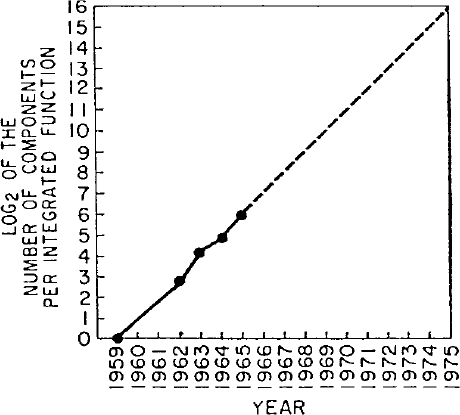
\includegraphics[width=0.5\textwidth]{./img/moore_orig.png}
\caption{\label{HW_moore_orig}La \emph{Ley de Moore}, en su artículo publicado en 1965, prediciendo la miniaturización por diez años}
\end{figure}

Esto cambió hacia el 2005. Tras más de 40 años de cumplirse, el modelo
conocido como la \emph{Ley de Moore}, enunciando que cada dos años la
densidad de transistores por circuito integrado se duplicaría,
llevaba a velocidades de CPU que, en el ámbito comercial, excedían los
3GHz, lo cual presentaba ya problemas serios de calentamiento. Además,
el diferencial de velocidad con el acceso a memoria era cada vez más
alto. Esto motivó a que las principales compañías productoras de los CPU
cambiaran de estrategia, introduciendo chips que son, para propósitos
prácticos, \emph{paquetes} con 2 o más procesadores dentro.

\begin{figure}[htb]
\centering
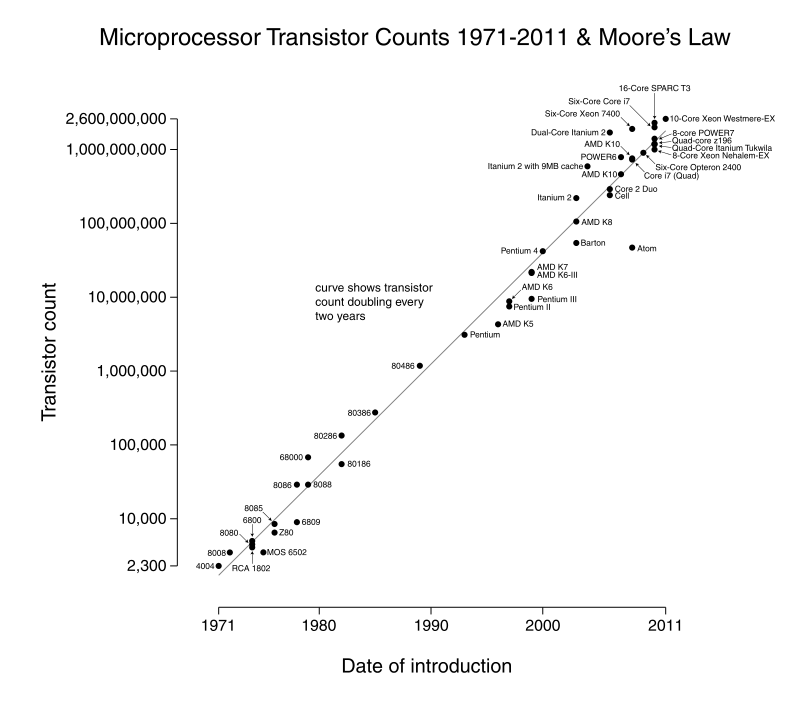
\includegraphics[width=0.7\textwidth]{./img/gnuplot/ley_de_moore.png}
\caption{\label{HW_ley_de_moore}La \emph{Ley de Moore} se sostiene al día de hoy: conteo de transistores por procesador de 1971 al 2012}
\end{figure}

Con este cambio, el \emph{reloj} de los procesadores se ha mantenido casi
sin cambios, cerca de 1GHz, pero el rendimiento de los equipos sigue
aumentando. Sin embargo, los programadores de sistemas operativos y
programas de aplicación ya no pueden ignorar esta complejidad
adicional.

Se denomina \emph{multiprocesamiento simétrico} (típicamente abreviado SMP)
a la situación en la que todos los procesadores del sistema son
iguales y pueden realizar en el mismo tiempo las mismas
operaciones. Todos los procesadores del sistema tienen acceso a la
misma memoria (aunque cada uno puede tener su propio \emph{caché}, lo cual
obliga a mantener en mente los puntos relacionados con la \emph{coherencia de caché} abordados en la sección anterior).

Existe también el \emph{multiprocesamiento asimétrico}; dependiendo de la
implementación, la asimetría puede residir en diferentes puntos. Puede
ir desde que los procesadores tengan una \emph{arquitectura} distinta
(típicamente dedicada a una tarea específica), en cuyo caso 
pueden verse como \emph{coprocesadores} o \emph{procesadores coadyuvantes}, casi
computadoras independientes contribuyendo sus resultados a un mismo
cómputo. Hoy en día, este sería el caso de las tarjetas gráficas 3D,
que son computadoras completas con su propia memoria y
responsabilidades muy distintas del sistema central.

Es posible tener diferentes procesadores con la misma arquitectura
pero funcionando a diferente frecuencia. Esto conlleva una fuerte
complejidad adicional, y no se utiliza hoy en día.

Por último, existen los diseños de \emph{Acceso No-Uniforme a Memoria}
(\emph{Non-Uniform Memory Access}, \emph{NUMA}). En este esquema, cada
procesador tiene \emph{afinidad} con bancos específicos de memoria — para
evitar que los diferentes procesadores estén esperando al mismo tiempo
al bus compartido de memoria, cada uno tiene acceso exclusivo a su
área. Los sistemas NUMA pueden ubicarse como en un punto intermedio
entre el procesamiento simétrico y el cómputo distribuído, y puede ser
visto como un \emph{cómputo distribuído fuertemente acoplado}.
\subsection{Cómputo distribuído}
\label{sec-2-9-2}


Se denomina cómputo distribuído a un proceso de cómputo realizado
entre computadoras independientes, o, más formalmente, entre
procesadores que \emph{no comparten memoria} (almacenamiento primario).
Puede verse que un equipo de diseño NUMA está a medio camino entre una
computadora multiprocesada y el cómputo distribuído.

Hay diferentes modelos para implementar el cómputo distribuído,
siempre basados en la transmisión de datos sobre una \emph{red}. Estos son
principalmente:

\begin{description}
\item[\emph{Cúmulos} (clusters)] Computadoras conectadas por una red local
     (de alta velocidad), ejecutando cada una su propia instancia de
     sistema operativo. Pueden estar orientadas al \emph{alto rendimiento},
     \emph{alta disponibilidad} o al \emph{balanceo de cargas} (o a una 
     combinación de estas). Típicamente son equipos homogéneos, y 
     dedicados a la tarea en cuestión.
\item[\emph{Mallas} (Grids)] Computadoras distribuídas geográficamente y
     conectadas a través de una red de comunicaciones. Las
     computadoras participantes pueden ser heterogéneas (en
     capacidades y hasta en arquitectura); la comunicación tiene que
     adecuarse a enlaces de mucha menor velocidad que en el caso de un
     cluster, e incluso presentar la elasticidad para permitir las
     conexiones y desconexiones de nodos en el transcurso del
     cómputo.
\item[Cómputo \emph{en la nube}] Un caso específico de cómputo distribuído
     con partición de recursos (al estilo del modelo
     cliente-servidor); este modelo de servicio está fuertemente
     orientado a la \emph{tercerización} de servicios específicos. A
     diferencia del modelo cliente-servidor tradicional, en un entorno
     de cómputo en la nube lo más común es que tanto el cliente como
     el servidor sean procesos que van integrando la información,
     posiblemente por muchos pasos, y que sólo eventualmente llegarán
     a un usuario final. La implementación de cada uno de los
     servicios empleados deja de ser relevante, para volverse un
     servicio \emph{opaco}. Algunos conceptos relacionados son:
\begin{description}
\item[Servicios Web] Mecanismo de descripción de funcionalidad, así
                     como de solicitud y recepción de resultados,
                     basado en el estándar HTTP y contenido XML.
\item[Software como servicio] El proveedor ofrece una \emph{aplicación        completa y cerrada} sobre la red, \emph{exponiendo} únicamente su
       interfaz (API) de consultas.
\item[Plataforma como servicio] El proveedor ofrece la \emph{abstracción}
       de un entorno específico de desarrollo de modo que un equipo de
       programadores pueda \emph{desplegar} una aplicación desarrollada
       sobre dicha plataforma tecnológica. Puede ser visto como un
       conjunto de piezas de infraestructura sobre un servidor
       administrado centralmente.
\item[Infraestructura como servicio] El proveedor ofrece computadoras
       completas (en hardware real o máquinas virtuales); la principal
       ventaja de esta modalidad es que los usuarios, si bien retienen
       la capacidad plena de administración sobre sus \emph{granjas},
       tienen mucho mayor flexibilidad para aumentar o reducir el
       consumo de recursos (y por tanto, el pago) según la demanda que
       alcancen.
\end{description}
El tema del cómputo en la nube va muy de la mano de la
  virtualización, que se abordará en el apéndice \ref{sec-9}.
\end{description}
\subsection{Amdahl y Gustafson: ¿qué esperar del paralelismo?}
\label{sec-2-9-3}


Al programar una aplicación de forma que aproveche al paralelismo
(esto es, diseñarla para que realice en distintos procesadores o nodos
sus \emph{porciones paralelizables}) ¿cuál es el incremento al rendimiento
que se puede esperar?

En 1967, Gene Amdahl presentó un artículo\footnote{\href{http://turing.eas.asu.edu/cse520fa08/Alaw.pdf}{Validity of the Single Processor Approach to Achieving Large Scale Computing Capabilities},
Amdahl, 1967 } en que indica los límites máximos en que resultará la
programación multiprocesada ante determinado programa: parte de la
observación de que aproximadamente 40\% del tiempo de ejecución de un
programa se dedicaba a administración y mantenimiento de los datos,
esto es, a tareas secuenciales.

Si únicamente el 60\% del tiempo de procesamiento es susceptible, pues,
de ser paralelizado, el rendimiento general del sistema no se
incrementará en una proporción directa con el número de procesadores,
sino que debe sumársele la porción estrictamente secuencial. Puesto en
términos más formales: la ganancia en la velocidad de ejecución de un
programa al ejecutarse en un entorno paralelo estará limitado por el
tiempo requerido por su fracción secuencial. Esto significa que, si
$T(1)$ representa al tiempo de ejecución del programa con un sólo
procesador y $T(P)$ al tiempo de ejecución con $P$ procesadores, y si
$t_s$ es el tiempo requerido para ejecutar la porción secuencial del
programa, y $t_p(P)$ el tiempo que requiere la ejecución de la porción
paralelizable, repartida entre $P$ procesadores, se puede hablar de una
ganancia $g$ en términos de:

$$g = \frac{T(1)}{T(P)} = \frac{t_s + t_p(1)}{t_s + \frac{t_p(1)}{P}}$$

\begin{figure}
\centering
\subfigure[Procesadores: 1, $t=500$ \label{HW_amdahl_1}]{\hskip 2em \includegraphics[height=0.33\textheight]{img/dot/amdahl_1.png} \hskip 2em}
\hfill
\subfigure[Procesadores: 2, $t=400$, ganancia: 1.25x \label{HW_amdahl_2}]{\includegraphics[height=0.33\textheight]{img/dot/amdahl_2.png} \hskip 1em}
\hfill
\subfigure[Procesadores: 4, $t=350$, ganancia: 1.4x \label{HW_amdahl_4}]{\includegraphics[height=0.33\textheight]{img/dot/amdahl_4.png}}
\caption {Ley de Amdahl: ejecución de un programa con 500 unidades de tiempo total de trabajo con uno, dos y cuatro procesadores.}
\label{HW_amdahl}
\end{figure}


Esta observación, conocida como la \emph{Ley de Amdahl}, llevó a que por
varias décadas el cómputo paralelo fuera relegado al cómputo de
propósito específico, para necesidades muy focalizadas en soluciones
altamente paralelizables, como el cómputo científico.

En términos del ejemplo presentado en la figura \ref{HW_amdahl}, se ve
un programa que, ejecutado secuencialmente, resulta en $T=500$. Este
programa está dividido en tres secciones secuenciales, de $t=100$ cada
una, y dos secciones paralelizables, totalizando $t=100$ cada una,
como se puede ver al representar una ejecución estrictamente
secuencial (\ref{HW_amdahl_1}).

Al agregar un procesador adicional (\ref{HW_amdahl_2}), se obtiene una
ganancia de 1.25x — la ejecución se completa en $T=400$ (con
$g=1.25$). Las secciones paralelizables sólo toman un tiempo \emph{externo}
de 50 cada una, dado que la carga fue repartida entre dos unidades de
ejecución. Al ejecutar con cuatro procesadores (\ref{HW_amdahl_4}), si
bien se sigue notando mejoría, esta apenas lleva a $T=350$,
con $g=1.4$.

Si el código fuera infinitamente paralelizable, y se ejecutase este
programa en una computadora con un número infinito de procesadores,
este programa no podría ejecutarse en menos de $T=300$, lo cual 
presentaría una ganancia de apenas $g=1.66$. Esto es, al agregar
procesadores adicionales, rápidamente se llegaría a un crecimiento
asintótico — el comportamiento descrito por la Ley de Amdahl es
frecuentemente visto como una demostración de que el desarrollo de
sistemas masivamente paralelos presenta \emph{rendimientos decrecientes}.

\begin{figure}[htb]
\centering
\includegraphics[width=0.6\textwidth]{./img/gnuplot/amdahl.png}
\caption{\label{HW_amdahl_porcentajes}Ganancia máxima al paralelizar un programa, según la Ley de Amdahl}
\end{figure}

Si bien el ejemplo que se acaba de presentar resulta poco optimizado, con sólo
un 40\% de código paralelizable, se puede ver en la gráfica
\ref{HW_amdahl_porcentajes} que el panorama no cambia tan fuertemente
con cargas típicas. Un programa relativamente bien optimizado, con 80\%
de ejecución paralela, presenta un crecimiento atractivo en la región
de hasta 20 procesadores, y se estaciona apenas arriba de una ganancia
de 4.5 a partir de los 40.\footnote{De un máximo de 5 al que puede
alcanzar con un número infinito de procesadores } Incluso el hipotético
95\% llega a un tope en su crecimiento, imposibilitado de alcanzar una
ganancia superior a 20.

Dado que el factor económico resulta muy importante para construir
computadoras masivamente paralelas,\footnote{Dado que los componentes más
caros son necesariamente los procesadores } y que se ve claramente que
el poder adicional que da cada procesador es cada vez menor, la
Ley de Amdahl resultó (como ya se mencionó) en varias décadas de mucho
mayor atención a la miniaturización y aumento de reloj, y no al
multiprocesamiento.

Fue hasta 1988 que John Gustafson publicó una observación a esta
ley\footnote{\href{http://www.johngustafson.net/pubs/pub13/amdahl.htm}{Reevaluating Amdahl's Law}, John L. Gustafson, Communications
of the ACM, vol. 31, mayo de 1988 } que, si bien no la invalida,
permite verla bajo una luz completamente diferente y mucho más
optimista. Gustafson publicó este artículo corto tras haber obtenido
ganancias superiores a 1020 en una supercomputadora con 1024
procesadores — un incremento casi perfectamente lineal al número de
procesadores. Sí, respondiendo a una carga altamente optimizada, pero
no por eso menos digna de análisis.

El argumento de Gustafson es que al aumentar el número de
procesadores, típicamente se verá una modificación \emph{al problema mismo}. Citando de su artículo (traducción propia),

\begin{quote}
(\ldots{})Asumen implícitamente que el tiempo que se ejecuta en paralelo es
independiente del número de procesadores, \emph{lo cual virtualmente nunca ocurre de este modo}. Uno no toma un problema de tamaño fijo para
ejecutarlo en varios procesadores como no sea para hacer un
ejercicio académico; en la práctica, \emph{el tamaño del problema crece con el número de procesadores}. Al obtener procesadores más poderosos, el
problema generalmente se expande para aprovechar las facilidades
disponibles. Los usuarios tienen control sobre cosas como la
resolución de la malla, el número de pasos, la complejidad de los
operadores y otros parámetros que usualmente se ajustan para permitir
que el programa se ejecute en el tiempo deseado. Por tanto, podría ser más
realista que el \emph{tiempo de ejecución}, no el \emph{tamaño del problema}, es
constante.
\end{quote}

Lo que escribe Gustafson se traduce a que es posible obtener la
eficiencia deseada de cualquier cantidad de procesadores \emph{aumentando suficientemente el tamaño del problema}. Al enfrentarse explícitamente
con el \emph{bloqueo mental} contra el paralelismo masivo que nació de esta
lectura errónea de lo comentado por Amdahl, su artículo sencillo y de
apenas más de una cuartilla de extensión cambió la percepción acerca
de la utilidad misma del paralelismo masivo.
\section{Otros recursos}
\label{sec-2-10}


\begin{itemize}
\item \emph{Can programming be liberated from the von Neumann style?: a   functional style and its algebra of programs}
  \otrorec{https://dl.acm.org/citation.cfm?doid=359576.359579}
  John Backus, 1978; Communications of the ACM
\item \emph{Cramming more components onto integrated circuits}
  \otrorec{http://cs.utexas.edu/~fussell/courses/cs352h/papers/moore.pdf}
  Gordon E. Moore, 1965; Proceedings of the IEEE
\item \emph{An Introduction to the Intel® QuickPath Interconnect}
  \otrorec{http://www.intel.com/content/www/us/en/io/quickpath-technology/quick-path-interconnect-introduction-paper.html}
  Intel, 2009 (Document Number: 320412-001US)
\item \emph{Intel® Desktop Board D875PBZ Technical Product Specification}
  \otrorec{http://downloadmirror.intel.com/15199/eng/D875PBZ_TechProdSpec.pdf}
  (Intel, 2003)
\end{itemize}
\chapter{Administración de procesos}
\label{sec-3}
\section{Concepto y estados de un proceso}
\label{sec-3-1}
\label{PROC}


En un sistema multiprogramado o de tiempo compartido, un \emph{proceso} es
la imagen en memoria de un programa, junto con la información
relacionada con el estado de su ejecución.

Un programa es una \emph{entidad pasiva}, una lista de instrucciones; un
proceso es una \emph{entidad activa}, que –empleando al programa– define la
actuación que tendrá el sistema.

En contraposición con \emph{proceso}, en un sistema por lotes se habla de
\emph{tareas}. Una tarea requiere mucha menos estructura, típicamente
basta con guardar la información relacionada con la \emph{contabilidad} de
los recursos empleados. Una tarea no es interrumpida en el transcurso
de su ejecución. Ahora bien, esta distinción no es completamente
objetiva — y se pueden encontrar muchos textos que emplean
indistintamente una u otra nomenclatura.

Si bien el sistema brinda la \emph{ilusión} de que muchos procesos se
están ejecutando al mismo tiempo, la mayor parte de ellos típicamente
está esperando para continuar su ejecución — en un momento
determinado sólo puede estar ejecutando sus instrucciones un número
de procesos igual o menor al número de procesadores que tenga el sistema.

En este capítulo se desarrollan los conceptos relacionados con
procesos, hilos, concurrencia y sincronización — Las técnicas y
algoritmos que emplea el sistema operativo para determinar cómo y en
qué orden hacer los cambios de proceso que nos brindan la ilusión de
simultaneidad se abordarán en el capítulo \ref{sec-4}.
\subsection{Estados de un proceso}
\label{sec-3-1-1}
\label{PROC_estados_de_un_proceso}


Un proceso, a lo largo de su vida, alterna entre diferentes \emph{estados}
de ejecución. Estos son:

\begin{description}
\item[Nuevo] Se solicitó al sistema operativo la creación de un proceso,
           y sus recursos y estructuras están siendo creadas.
\item[Listo] Está listo para iniciar o continuar su ejecución pero el sistema
		no le ha asignado un procesador.
\item[En ejecución] El proceso está siendo ejecutado en este
                  momento. Sus instrucciones están siendo procesadas
                  en algún procesador.
\item[Bloqueado] En espera de algún evento para poder continuar
               su ejecución (aun si hubiera un procesador disponible,
               no podría avanzar).
\item[Zombie] El proceso ha finalizado su ejecución, pero el sistema
            operativo debe realizar ciertas operaciones de limpieza
            para poder eliminarlo de la lista.\footnote{Estas operaciones
            pueden incluir notificar al proceso padre, cerrar las
            conexiones de red que tenía activas, liberar memoria, etc. }
\item[Terminado] El proceso terminó de ejecutarse; sus estructuras están
               a la espera de ser \emph{limpiadas} por el sistema operativo
\end{description}

\begin{figure}[htb]
\centering
\includegraphics[width=0.4\textwidth]{./img/dot/estados_proceso.png}
\caption{\label{PROC_estados_proceso}Diagrama de transición entre los estados de un proceso}
\end{figure}
\subsection{Información asociada a un proceso}
\label{sec-3-1-2}


La información que debe manipular el sistema operativo relativa a cada
uno de los procesos actuales se suele almacenar en una estructura llamada
\emph{bloque de control de proceso} (\emph{PCB} - \emph{Process Control Block}). El 
PCB incluye campos como:

\begin{description}
\item[Estado del proceso] El estado actual del proceso.
\item[Contador de programa] Cuál es la siguiente instrucción a ser
     ejecutada por el proceso.
\item[Registros del CPU] La información específica del estado del CPU
     mientras el proceso está en ejecución (debe ser respaldada y
     restaurada cuando se registra un cambio de estado).
\item[Información de planificación (scheduling)] La prioridad del
     proceso, la \emph{cola} en que está agendado, y demás información que
     puede ayudar al sistema operativo a planificar los procesos; se
     profundizará el tema en el capítulo \ref{sec-4}.
\item[Información de administración de memoria] La información de mapeo
     de memoria (páginas o segmentos, dependiendo del sistema
     operativo), incluyendo la pila (\emph{stack}) de llamadas. Se abordará
     el tema en el capítulo \ref{sec-5}.
\item[Información de contabilidad] Información de la utilización de
     recursos que ha tenido este proceso — Puede incluir el tiempo
     total empleado y otros (\emph{de usuario}, cuando el procesador va
     avanzando sobre las instrucciones del programa propiamente, \emph{de      sistema} cuando el sistema operativo está atendiendo las
     solicitudes del proceso), uso acumulado de memoria y dispositivos, etc.
\item[Estado de E/S] Listado de dispositivos y archivos asignados que el
                   proceso tiene \emph{abiertos} en un momento dado.
\end{description}
\section{Procesos e hilos}
\label{sec-3-2}


Como se vio, la cantidad de información que el sistema operativo debe
manejar acerca de cada proceso es bastante significativa. Si cada vez
que el \emph{planificador} elige qué proceso pasar de \emph{Listo} a \emph{En ejecución} debe considerar buena parte de dicha información, la simple
transferencia de todo esto entre la memoria y el procesador podría
llevar a un desperdicio \emph{burocrático}\footnote{Entendiendo \emph{burocrático}
como el tiempo que se pierde en asuntos administrativos. Recordar
que el tiempo que consume el sistema operativo en administración es
tiempo perdido para el uso real, productivo del equipo. } de
recursos. Una respuesta a esta problemática fue la de utilizar los
\emph{hilos de ejecución}, a veces conocidos como \emph{procesos ligeros}
(\emph{LWP}, \emph{Lightweight processes}).

Cuando se consideran procesos basados en un modelo de hilos, se puede
proyectar en sentido inverso que todo proceso es como un sólo hilo de
ejecución. Un sistema operativo que no ofreciera soporte expreso a los
hilos los planificaría exactamente del mismo modo.

Pero visto desde la perspectiva del proceso hay una gran diferencia:
si bien el sistema operativo se encarga de que cada proceso tenga una
visión de virtual exclusividad sobre la computadora, todos los hilos
de un proceso comparten un sólo espacio de direccionamiento en memoria
y los archivos y dispositivos abiertos. Cada uno
de los hilos se ejecuta de forma (aparentemente) secuencial y maneja
su propio contador de programa y pila (y algunas estructuras adicionales,
aunque mucho más ligeras que el PCB).
\subsection{Los hilos y el sistema operativo}
\label{sec-3-2-1}
\label{PROC_tipos_de_hilos}


La programación basada en hilos puede hacerse
completamente y de forma transparente en espacio de usuario (sin
involucrar al sistema operativo). Estos hilos se llaman \emph{hilos de usuario} (\emph{user threads}), y muchos lenguajes de programación los
denominan \emph{hilos verdes} (\emph{green threads}). Un caso de uso interesante
es en sistemas operativos mínimos (p. ej. para dispositivos embebidos)
capaces de ejecutar una máquina virtual de alguno de esos lenguajes:
si bien el sistema operativo no maneja multiprocesamiento, a través de
los hilos de usuario se crean procesos con multitarea interna.

Los procesos que implementan hilos ganan un poco en el rendimiento
gracias a no tener que reemplazar al PCB activo cuando intercalan la 
ejecución de sus diferentes hilos; pero además de esto, ganan mucho
más por la ventaja de compartir espacio de memoria sin tener que
establecerlo explícitamente a través de \emph{mecanismos de comunicación entre procesos} (\emph{IPC} — \emph{Inter Process Communications}). Dependiendo
de la plataforma, a veces los hilos de usuario inclusive utilizan
multitarea cooperativa para pasar el control dentro de un mismo
proceso. Cualquier llamada al sistema \emph{bloqueante} (como obtener datos
de un archivo para utilizarlos inmediatamente) interrumpirá la
ejecución de \emph{todos} los hilos de ese proceso, dado que
el control de ejecución es entregado al sistema operativo quien en
este caso no conoce nada sobre los hilos.


Continuando con el desarrollo histórico de este mecanismo, el
siguiente paso fue la creación de hilos \emph{informando} al sistema
operativo, típicamente denominados \emph{hilos de kernel} (\emph{kernel threads}). Esto se hace a través de bibliotecas de sistema que los
implementan de forma estándar para los diferentes sistemas operativos
o arquitecturas  (p. ej. \texttt{pthreads} para POSIX o \texttt{Win32\_Thread} para
Windows). Estas bibliotecas aprovechan la comunicación con el
sistema operativo tanto para solicitudes de recursos (p. ej. un proceso
basado en hilos puede beneficiarse de una ejecución verdaderamente
paralela en sistemas multiprocesador) como para una gestión de
recursos más comparable con una situación de multiproceso estándar.
\subsection{Patrones de trabajo con hilos}
\label{sec-3-2-2}


Hay tres patrones en los que caen generalmente los modelos de hilos;
se puede emplear más de uno de estos patrones en diferentes áreas de
nuestra aplicación, e incluso se pueden \emph{anidar} (esto es, se podría
tener una \emph{línea de ensamblado} dentro de la cual uno de los pasos sea
un \emph{equipo de trabajo}):

\begin{description}
\item[Jefe / trabajador] Un hilo tiene una tarea distinta de todos los
     demás: el hilo \emph{jefe} genera o recopila tareas para realizar, las
     separa y se las entrega a los hilos \emph{trabajadores}.

     Este modelo es el más común para procesos que implementan
     servidores (es el modelo clásico del servidor Web \emph{Apache}) y
     para aplicaciones gráficas (GUIs), en que hay una porción del
     programa (el hilo \emph{jefe}) esperando a que ocurran eventos
     externos. El jefe realiza poco trabajo, se limita a \emph{invocar} a
     los trabajadores para que hagan el trabajo \emph{de verdad}; como mucho,
     puede llevar contabilidad de los trabajos realizados.

     Típicamente, los hilos trabajadores realizan su operación, posiblemente
     notifican al \emph{jefe} de su trabajo, y \emph{finalizan} su ejecución.

     \begin{figure}[htb]
     \centering
     \includegraphics[width=0.4\textwidth]{./img/dot/jefe_trabajador.png}
     \caption{\label{PROC_jefe_trabajador}Patrón de hilos jefe/trabajador}
     \end{figure}
\end{description}


\begin{description}
\item[Equipo de trabajo] al iniciar la porción multihilos del proceso,
     se crean muchos hilos idénticos, que realizarán las mismas tareas
     sobre diferentes datos. Este modelo es muy frecuentemente
     utilizado para cálculos matemáticos (p. ej.: criptografía,
     render, álgebra lineal). Puede combinarse con un estilo jefe/trabajador para irle
     dando al usuario una previsualización del resultado de su
     cálculo, dado que éste se irá ensamblando progresivamente, pedazo
     por pedazo.

     Su principal diferencia con el patrón \emph{jefe/trabajador}
     consiste en que el trabajo a realizar por cada uno de los hilos
     se plantea desde principio, esto es, el paso de \emph{división de      trabajo} no es un hilo más, sino que prepara los datos para que
     éstos sean lanzados en \emph{paralelo}. Estos datos no son resultado de
     \emph{eventos independientes} (como en el caso anterior), sino 
     partes de un sólo cálculo. Por consecuencia, resulta natural que
     en este modelo los resultados generados por los diferentes hilos
     son \emph{agregados} o \emph{totalizados} al terminar su procesamiento. Los
     hilos no \emph{terminan}, sino que \emph{son sincronizados} y luego continúan la
     ejecución lineal.

     \begin{figure}[htb]
     \centering
     \includegraphics[width=0.5\textwidth]{./img/dot/equipo_trab.png}
     \caption{\label{PROC_equipo_trab}Patrón de hilos \emph{Equipo de trabajo}}
     \end{figure}
\end{description}


\begin{description}
\item[Línea de ensamblado] si una tarea larga puede dividirse en pasos
     sobre bloques de la información total a procesar, cada hilo puede
     enfocarse a hacer sólo un paso y pasarle los datos a otro hilo
     conforme vaya terminando. Una de las principales ventajas de este
     modelo es que nos ayuda a mantener rutinas simples de comprender,
     y permite que el procesamiento de datos continúe incluso si parte
     del programa está bloqueado esperando E/S.

     Un punto importante a tener en cuenta en una línea de ensamblado
     es que, si bien los hilos trabajan de forma secuencial, pueden
     estar ejecutándose paralelamente sobre bloques consecutivos de
     información, eventos, etc.

     Este patrón es claramente distinto de los dos anteriormente
     presentados; si bien en los anteriores los diferentes hilos (a
     excepción del hilo \emph{jefe}) eran casi siempre idénticos -aunque
     operando sobre distintos conjuntos de datos-, en este caso son
     todos completamente distintos.

     \begin{figure}[htb]
     \centering
     \includegraphics[width=0.6\textwidth]{./img/dot/linea_ensamblado.png}
     \caption{\label{PROC_linea_ensamblado}Patrón de hilos \emph{Línea de ensamblado}}
     \end{figure}
\end{description}
\section{Concurrencia}
\label{sec-3-3}
\label{PROC_concurrencia}
\subsection{Introducción}
\label{sec-3-3-1}


Desde un punto de vista formal, la \emph{concurrencia} no se refiere a dos
o más eventos que ocurren a la vez sino a dos o más eventos cuyo orden
es \emph{no determinista}, esto es, eventos acerca de los cuales \emph{no se puede predecir el orden relativo en que ocurrirán}. Si bien dos
procesos (o también dos hilos) completamente independientes entre sí
ejecutándose simultáneamente son dos procesos concurrentes, la
concurrencia se ocupa principalmente de procesos cuya ejecución está
vinculada de alguna manera (p. ej.: dos procesos que comparten cierta
información o que dependen uno del otro).

Aunque una de las tareas principales de los sistemas operativos es dar
a cada proceso la ilusión de que se está ejecutando en una computadora
dedicada, de modo que el programador no tenga que pensar en la
competencia por recursos, a veces un programa requiere interactuar con
otros: parte del procesamiento puede depender de datos
obtenidos en fuentes externas, y la cooperación con hilos o
procesos externos es fundamental.

Se verá que pueden aparecer muchos problemas cuando se estudia la
interacción entre hilos del mismo proceso, la sincronización entre
distintos procesos, la asignación de recursos por parte del sistema operativo a
procesos simultáneos, o incluso cuando interactuan usuarios de
diferentes computadoras de una red — se presentarán distintos conceptos
relacionados con la concurrencia utilizando uno de esos escenarios,
pero muchos de esos conceptos en realidad son independientes del
escenario: más bien nos ocupa la relación entre procesos que deben
compartir recursos o deben sincronizar sus tareas.

Para presentar los problemas y conceptos relacionados con la
concurrencia suelen utilizarse algunos problemas clásicos, que
presentan casos particulares muy simplificados, y puede encontrárseles
relación con distintas cuestiones que un programador enfrentará en
la vida real. Cada ejemplo presenta uno o más
conceptos. Se recomienda comprender bien el ejemplo, el problema y la
solución y desmenuzar buscando los casos límite como ejercicio antes de pasar al siguiente
caso. También podría ser útil imaginar en qué circunstancia un
sistema operativo se encontraría en una situación similar.

Para cada problema se mostrará \emph{una forma} de resolverlo 
aunque en general hay más de
una solución válida. Algunos de estos problemas fueron originalmente
planteados como justificación del desarrollo de las estructuras de
control presentadas o de nuevos paradigmas de concurrencia y muchos
son aun objeto de debate e investigación.

Para profundizar más en este tema, se recomienda el libro «\href{http://greenteapress.com/semaphores/}{The little book of semaphores}» de Allen Downey (2008).
En este libro (de libre descarga) se encuentran muchos ejemplos
que ilustran el uso de semáforos no sólo para resolver problemas de
sincronización, sino como un mecanismo simple de comunicación entre
procesos. También se desarrollan distintas soluciones para los
problemas clásicos (y no tan clásicos).
\subsection{Problema: el jardín ornamental}
\label{sec-3-3-2}
\label{PROC_problemas_clasicos}
\subsubsection{Descripción del problema}
\label{sec-3-3-2-1}


Un gran jardín ornamental se abre al público para que todos puedan
apreciar sus fantásticas rosas, arbustos y plantas acuáticas. Por
supuesto, se cobra una módica suma de dinero a la entrada para lo cual
se colocan dos torniquetes, uno en cada una de sus dos entradas. Se desea
conocer cuánta gente ha ingresado al jardín así que se instala una
computadora conectada a ambos torniquetes: cada torniquete envía una
señal cuando una persona ingresa al jardín. Se realiza un modelo
simplificado de la situación, así que no se estudiarán los
detalles del hardware utilizado. Aquí es importante notar que los dos
torniquetes son objetos que existen y se comportan en paralelo e independientemente: los
eventos que generan no tienen un orden predecible. Es decir, que
cuando se escriba el software no se sabe en qué momento llegará cada
visitante ni qué torniquete utilizará.

Se simulará un experimento en el que 20 visitantes ingresan por cada
torniquete. Al final de la simulación deberá haber 40 visitantes
contados. Una implementación tentativa podría ser la
siguiente:\footnote{Se utiliza una versión
ficticia del lenguaje C para el ejemplo, evitando entrar en los
detalles de sintáxis de un lenguaje concurrente. }


\begin{verbatim}
int cuenta; 

proceso torniquete1() {
        int i;
        for(i=0;i<20;i++) {
                cuenta = cuenta + 1;
        }
}

proceso torniquete2() {
        int i;
        for(i=0;i<20;i++) {
                cuenta = cuenta + 1;
        }
}

main() {
        cuenta = 0;
        /* Lanzar ambos procesos concurrentemente*/
        concurrentemente { //
                torniquete1();
                torniquete2();
        }
        /* Esperar a que ambos finalicen */
        esperar(torniquete1);
        esperar(torniquete2);
        printf("Cuenta: %d\n", cuenta);
}
\end{verbatim}

Como se ve el problema es muy sencillo. Sin embargo, al
intentar ejecutar repetidas veces ese programa muy de vez en cuando el
resultado no tiene el valor 40. Si se modifica el programa para
utilizar un solo torniquete, \texttt{cuenta} siempre tiene el valor correcto
(20).

¿Qué es lo que está ocurriendo? La mayor parte de los lenguajes de
programación convierten cada instrucción en una serie más o menos
larga de operaciones de máquina (instrucciones ensamblador). De modo,
que una instrucción aparentemente simple como \texttt{cuenta = cuenta + 1}
habitualmente implica varias operaciones de más bajo nivel (las instrucciones
de ejemplo corresponden a arquitecturas Intel x86):

\begin{description}
\item[\texttt{LEER}] Leer \texttt{cuenta} desde la memoria (p. ej. \texttt{mov \$cuenta, \%rax}).
\item[\texttt{INC}] Incrementar el registro (p. ej. \texttt{add \$1, \%rax}).
\item[\texttt{GUARDAR}] Guardar el resultado nuevamente en memoria (p. ej. \texttt{mov 	       \%rax, \$cuenta}).
\end{description}

En un sistema operativo multitarea cuando un proceso agota su porción
de tiempo de procesador (quantum) o detiene su ejecución por otra
razón, los valores almacenados en registros se preservan (junto con la
información sobre el proceso) para poder restaurarlo cuando la
ejecución continúe (de esta forma se provee la ilusión de la
multitarea en sistemas de un solo núcleo). Así, en el problema del
Jardín Ornamental cada torniquete tiene su propia copia de los valores
en los registros. Sin embargo, se supone que el resto de la memoria es
compartida (en particular, se utiliza ese hecho para llevar la cuenta
de personas que ingresan).

Si se considera lo que ocurre cuando dos procesos (p. ej. \texttt{torniquete1}
y \texttt{torniquete2}) ejecutan la instrucción \texttt{cuenta = cuenta + 1} en un equipo con un
solo procesador, puede darse la siguiente secuencia de eventos. Se
considera que \texttt{cuenta} está inicialmente en \texttt{0}.

\begin{enumerate}
\item \texttt{cuenta = 0}
\item \texttt{torniquete1}: \texttt{LEER} (resultado: \texttt{rax} de $p_1$ = 0, \texttt{cuenta = 0})
\item \texttt{torniquete1}: \texttt{INC} (resultado: \texttt{rax} de $p_1$ = 1, \texttt{cuenta = 0})
\item \texttt{torniquete1}: \texttt{GUARDAR} (resultado: \texttt{rax} de $p_1$ = 1, \texttt{cuenta = 1})
\item El sistema operativo decide cambiar de tarea, suspende \texttt{torniquete1} y
   continúa con \texttt{torniquete2}.
\item \texttt{torniquete2}: \texttt{LEER} (resultado: \texttt{rax} de $p_2$ = 1, \texttt{cuenta = 1})
\item \texttt{torniquete2}: \texttt{INC} (resultado: \texttt{rax} de $p_2$ = 2, \texttt{cuenta = 1})
\item \texttt{torniquete2}: \texttt{GUARDAR} (resultado: \texttt{rax} de $p_2$ = 2, \texttt{cuenta = 2})
\end{enumerate}

Se puede ver que ambos procesos realizaron sus instrucciones para
incrementar el contador en 1 y el resultado final fue que la cuenta se
incrementó en dos unidades.

Pero, también puede darse la siguiente secuencia de eventos durante la
ejecución de estas instrucciones:

\begin{enumerate}
\item \texttt{cuenta = 0}
\item \texttt{torniquete1}: \texttt{LEER} 		(resultado: \texttt{rax} de $p_1$ = 0, \texttt{cuenta = 0})
\item \texttt{torniquete1}: \texttt{INC} 		(resultado: \texttt{rax} de $p_1$ = 1, \texttt{cuenta = 0})
\item El sistema operativo decide cambiar de tarea, suspende \texttt{torniquete1} y
   continúa con \texttt{torniquete2}.
\item \texttt{torniquete2}: \texttt{LEER} 		(resultado: \texttt{rax} de $p_2$ = 1, \texttt{cuenta = 1})
\item \texttt{torniquete2}: \texttt{INC} 		(resultado: \texttt{rax} de $p_2$ = 2, \texttt{cuenta = 1})
\item \texttt{torniquete2}: \texttt{GUARDAR} 		(resultado: \texttt{rax} de $p_2$ = 2, \texttt{cuenta = 2})
\item El sistema operativo decide cambiar de tarea, suspende \texttt{torniquete2}
   y continua con \texttt{torniquete1}.
\item \texttt{torniquete1}: \texttt{GUARDAR} 		(resultado: \texttt{rax} de $p_1$ = 1, \texttt{cuenta = 1})
\end{enumerate}

Nuevamente ambos procesos ejecutaron sus instrucciones para
incrementar en 1 el contador. Sin embargo, ¡en este caso \texttt{cuenta}
tiene el valor 1!. A este problema también se lo conoce como \emph{problema de las actualizaciones múltiples}.

\begin{description}
\item[Esto parece muy específico] Si bien este análisis parece muy específico es fácil ver que la
  misma circustancia podría darse en un sistema de reserva de vuelos
  (p. ej.: puede que dos operadores vean un asiento vacío en su copia
  local de los asientos y ambos marquen el mismo asiento como ocupado)
  o con dos procesos que decidan cambiar simultáneamente datos en un
  archivo. Aquí las operaciones ya no son necesariamente operaciones
  internas de la máquina.
\item[¿Pero no es muy poco probable?] Por otro lado, uno podría pensar (con cierta cuota de razón) que la
  secuencia de eventos propuesta es muy poco probable: usualmente un
  sistema operativo ejecuta miles de instrucciones antes de cambiar de
  un proceso a otro. De hecho, en la práctica este problema es muy
  frecuentemente ignorado y los programas funcionan muy bien la mayoría
  de las veces. Esto permite ver una característica importante de los
  programas concurrentes: es muy usual que un programa funcione
  perfectamente la mayor parte del tiempo, pero de vez en cuando puede
  fallar. Subsecuentes ejecuciones con los mismos argumentos producen
  nuevamente el resultado correcto. Esto hace que los problemas de
  concurrencia sean muy difíciles de detectar y más aun de corregir. Es
  importante (y mucho más efectivo) realizar un buen diseño inicial de
  un programa concurrente en lugar de intentar arreglarlo cuando se
  detecta alguna falla. También es interesante notar que dependiendo del
  sistema, puede ser que alguna de las instrucciones sea muy lenta, en
  el caso de un sistema de reserva de asientos de aviones, las
  operaciones pueden durar un tiempo importante (p. ej.: desde que el
  operador muestra los asientos disponibles hasta que el cliente elige
  el asiento) haciendo mucho más probable que ocurra una secuencia no
  deseada.
\item[¿Vale la pena preocuparse?] A modo de ilustración de la gravedad del problema, estos son algunos
  valores para el resultado final de la variable \texttt{cuenta} cuando se
  ejecuta el programa anterior en Pascal-FC\footnote{http://www-users.cs.york.ac.uk/burns/pf.html }: 25 29 31 20 21 26 27
  18 31 35. Notesé que incluso uno de los valores es menor que \emph{20}
  (que es lo mínimo que cuenta cada torniquete). Es un ejercicio
  interesante pensar qué secuencia de eventos podría producir tal
  valor y cuál es el mínimo valor posible.
\item[Pero tenemos muchos núcleos] Otra cuestión que puede parecer artificiosa es que en el ejemplo hay
  un solo procesador o núcleo. Sin embargo, tener más de un procesador
  no sólo no soluciona el problema sino que lo empeora: ahora las
  operaciones de lectura o escritura pueden ejecutarse directamente en
  paralelo y aparecen nuevos problemas de coherencia de caché. En la
  siguiente discusión muchas veces se presupone que hay un solo
  procesador, sin que eso invalide la discusión para equipos
  multiprocesadores.
\end{description}
\subsubsection{Algunos conceptos de concurrencia}
\label{sec-3-3-2-2}


Antes de abordar posibles soluciones al problema presentado, se
presentan las definiciones de algunos conceptos importantes.

\begin{description}
\item[Operación atómica] Operación que requiere la garantía de que se
     ejecutará como una sóla unidad de ejecución, o fallará
     completamente, sin resultados o estados parciales observables por
     otros procesos o el entorno. Esto no necesariamente implica que
     el sistema no retirará el flujo de ejecución en medio de la
     operación, sino que \emph{el efecto de que se le retire el flujo} no
     llevará a comportamiento inconsistente.
\item[Condición de carrera] (En inglés, \emph{Race condition}) Categoría de errores de
     programación que involucra a dos procesos que fallan al comunicarse
     su estado mutuo, llevando a resultados inconsistentes. Es uno de
     los problemas más frecuentes y difíciles de depurar, y ocurre
     típicamente por no considerar la \emph{no atomicidad} de una operación
\item[Sección (o región) crítica] El área de código que requiere ser protegida de
     accesos simultáneos, donde se realiza la modificiación de datos
     compartidos.
\item[Recurso compartido] Un recurso que puede ser accedido desde más de
     un proceso. En muchos escenarios esto es un variable en memoria 
     (como \texttt{cuenta} en el jardín ornamental),
     pero podrían ser archivos, periféricos, etc\ldots{}
\end{description}

Dado que el sistema no tiene forma de saber cuáles instrucciones (o
áreas del código) deben funcionar de forma atómica, el programador debe asegurar
la atomicidad de forma explícita, mediante la sincronización de los
procesos. El sistema no debe permitir la ejecución de parte de esa
área en dos procesos de forma simultánea (sólo puede haber un proceso
en la sección crítica en un momento dado).
\begin{itemize}

\item ¿Y qué tiene que ver esto con el problema del Jardín Ornamental?\\
\label{sec-3-3-2-2-1}%
En el problema hay claramente un \emph{recurso compartido} que es la \texttt{cuenta}, así la
sección que modifica la cuenta es una \emph{sección crítica} y la operación
\texttt{cuenta = cuenta + 1} debe ser una \emph{operación atómica}. La secuencia de eventos que
se mostró es una \emph{condición de carrera}: el segundo torniquete presume
un estado (\texttt{cuenta = 0}) que no es el mismo que conoce el \texttt{torniquete1}
(\texttt{cuenta = 1}).

\end{itemize} % ends low level
\subsubsection{Soluciones posibles (y no tanto)}
\label{sec-3-3-2-3}


El planteamiento del problema del \emph{jardín ornamental} busca llevar al
lector a ir encontrando, a través de sucesivos refinamientos, los
mecanismos principales que se emplean para resolver –en general– los
problemas que implican el acceso concurrente a una sección crítica. Se
presentan a continuación, pues, los sucesivos \emph{intentos}.

\begin{description}
\item[Intento 1: No utilizar multitarea] En este sencillo ejemplo una posible solución es utilizar una sola
  entrada (o torniquete). Esto podría ser una solución en tanto que no
  haya mucha gente que haga cola para entrar. Sin embargo, en un sistema
  análogo de reserva de pasajes aereos no parece tener mucho sentido que
  todos los pasajeros deban ir a Japón a sacar su pasaje. Por otro lado,
  ya deberían ser claras las ventajas de la multitarea y el poseer
  distintos núcleos.
\item[Intento 2: Suspender la multitarea durante la sección crítica] Una versión más relajada de la alternativa anterior es suspender la
  multitarea durante la ejecución de la sección crítica. Así, un
  torniquete deberá hacer:


\begin{verbatim}
disable(); /* Suspender temporal las interrupciones */
cuenta = cuenta + 1;
enable(); /* Habilitar nuevamente las interrupciones */
\end{verbatim}
\end{description}

  Durante el lapso en el que las interrupciones están suspendidas no
  puede haber un cambio de contexto pues el planificador depende de la
  interrupción del reloj (salvo que el proceso realice una
  llamada bloqueante durante la región crítica).

  Esta solución puede resultar conveniente para sistemas sencillos, pero
  en un sistema multiusuario se torna inusable por varios motivos:

\begin{itemize}
\item Permitir que un programa de usuario deshabilite las interrupciones
    en un sistema operativo de propósito general involucra un gran
    problema de seguridad: cualquier usuario podría hacer un programa
    malicioso (o sencillamente erroneo) que deshabilite las
    interrupciones y suspenda indefinidamente el resto del sistema.
\item No funciona para sistemas distribuídos (como el sistema de reserva
    de pasajes aereos), ni siquiera para sistemas multinúcleo o
    multiprocesador, ya que las interrupciones se deshabilitan en un
    sólo núcleo (si bien también es posible detener a los demás
    procesadores, representa un costo demasiado alto).
\item Expone detalles de hardware y podría provocar mal funcionamiento de
    algún periférico si el procesamiento de la sección crítica es
    demasiado largo.
\item Intento 3: Utilizar una bandera ::
\end{itemize}
  Utilizar una bandera parece ser una solución muy sencilla: mediante
  una variable de bandera se indica si hay un proceso en la región crítica:


\begin{verbatim}
int bandera = 0; /* 0 => región crítica libre, 1 => ocupada */
int cuenta = 0;
/* ... */

/* Torniquete1 */
/* ... */
if (bandera) wait;
/* Aquí bandera=0 */
bandera = 1; /* Inicio de la sección crítica */
cuenta = cuenta + 1;
bandera = 0; /* Fin de la sección crítica */
\end{verbatim}

  Sin embargo esto no funciona, ahora puede darse la siguiente secuencia
  de eventos:

\begin{enumerate}
\item \texttt{bandera==0;}
\item \texttt{torniquete2}: \texttt{if (bandera) wait;}
\item Nuevo cambio de contexto
\item \texttt{torniquete1}: \texttt{if (bandera) wait;}
\item \texttt{torniquete1}: \texttt{bandera = 1;}
\item \texttt{torniquete2}: \texttt{bandera = 1;}
\item \texttt{torniquete2}: \texttt{cuenta = cuenta + 1;}
\item \texttt{torniquete1}: \texttt{cuenta = cuenta + 1; /* Ups, no se respetó la región crítica */}
\end{enumerate}

  Notar que el problema aquí es que la bandera también es un recurso
  compartido: lo único que ha cambiado es que ahora la sección crítica
  está en otro lugar. La solución funcionaría si se pudiera
  garantizar que la secuencia de operaciones se realizara atómicamente:


\begin{verbatim}
if (bandera) wait;
bandera = 1
\end{verbatim}

\begin{description}
\item[Intento 4: Manejar la bandera con instrucciones atómicas] Algunas arquitecturas de computadoras permiten realizar determinadas
  operaciones sencillas (como actualizar una bandera) de forma atómica
  (p. ej.: VAX tiene la instrucción \texttt{test\_and\_set} y el i386 tiene la
  instrucción \texttt{INC}.

  Usando esto, la solución es:


\begin{verbatim}
int bandera; /* 0 => desocupada */

while (++bandera != 1) {
    bandera--; /* Debe generar "INC" */
}
/* Sección crítica */
cuenta = cuenta + 1;

bandera--;
\end{verbatim}
\end{description}

  Esto funciona correctamente siempre que la operación \emph{++bandera} sea
  atómica.  Sin embargo, hay dos problemas a considerar: un proceso
  puede permanecer mucho tiempo repitiendo el ciclo:


\begin{verbatim}
while (++bandera!=1) {
    bandera--;
}
\end{verbatim}

  De hecho, si el sistema operativo decide darle alta prioridad a este
  proceso es posible que esté un tiempo infinito en este ciclo,
  impidiendo que otro proceso decremente la bandera. Y aún cuando el
  sistema operativo decida cambiar de proceso en el siguiente tic de
  reloj, es evidente que se podría aprovechar el procesador para hacer
  algo útil durante ese tiempo y que suspender el proceso de otra manera
  le da más posibilidad a otros procesos para que cambien la bandera. A
  esto se lo conoce como \emph{espera activa} o \emph{espera ocupada} (\emph{busy   waiting} en inglés) y es una situación que se desea evitar.

  El otro problema tiene que ver con el hardware: determinadas
  arquitecturas no permiten instrucciones que lean y actualicen en una
  única operación una dirección de memoria (se requiere una operación
  para leer y otra para escribir).  En particular, ninguna arquitectura
  RISC lo permite (p. ej.: SPARC, RS 6000, \ldots{}).

\begin{description}
\item[Intento 5: Utilizar turnos] Una alternativa para evitar el problema de la actualización múltiple a
  una bandera es utilizar turnos


\begin{verbatim}
int turno = 1; /* Inicialmente el turno es del proceso 1 */
\end{verbatim}
\end{description}
  Ahora el código del proceso 1 contendría algo como:


\begin{verbatim}
while (turno != 1) {
    esperar(); /* ¿Otro proceso? */
}
/* Sección crítica */
cuenta = cuenta + 1;
turno = 2;
\end{verbatim}

  Y el del proceso dos:


\begin{verbatim}
while (turno != 2) {
    esperar();
}
/* Sección crítica */
cuenta = cuenta + 1;
turno = 1;
\end{verbatim}

  Esto garantiza que no hay dos procesos en sección crítica. Pero nótese
  que hacer esto equivale a tener un solo torniquete: sólo podrá haber
  una persona ingresando a la vez\ldots{} o incluso peor, las personas
  deberán utilizar alternativamente los torniquetes. Así que si bien
  esto soluciona el problema de la actualización múltiple en realidad es
  una solución muy restrictiva: un proceso que no está en la sección
  crítica puede obligar a que otro proceso espere mucho tiempo para
  ingresar a la sección crítica. De aquí en más se buscarán soluciones en
  las que no ocurra esto.

\begin{description}
\item[Intento 6: Indicar la intención de entrar a la sección crítica] Para paliar los efectos de la solución anterior se puede intentar
  indicar si el otro proceso también está queriendo entrar en la sección
  crítica. El código sería:


\begin{verbatim}
int b1, b2;
/* ... */

/* Proceso 1: */
/* ... */
b1 = 1;
if (b2) {
    esperar();
}
/* Sección crítica */
cuenta = cuenta + 1;
b1 = 0;
/* ... */
/* Proceso 2: */
/* ... */
b2 = 1;
if (b1) {
    esperar();
}
/* Sección crítica */
cuenta = cuenta + 1;
b2 = 0;
/* ... */
\end{verbatim}
\end{description}

  Nuevamente aquí está garantizado que no puede haber dos procesos en la
  región crítica, pero este enfoque sufre de un problema grave: ambos
  procesos pueden bloquearse mutuamente (si el proceso 1 coloca su
  bandera en 1 y luego se cambia el control al proceso 2 quien también
  colocará su bandera en 1).
ORG-LIST-END-MARKER
\subsubsection{Una solución: el Algoritmo de Peterson}
\label{sec-3-3-2-4}


La primera solución a esta problema fue propuesta por Dekker
en 1957. Sin embargo su explicación es bastante extensa (aunque
perfectamente comprensible). Se presentará la solución
planteada por Peterson unos cuantos años más tarde: en 1970.

La solución está basada en una combinación de los intentos anteriores:
utilizar banderas para indicar qué proceso puede entrar, pero además
usa un turno para \emph{desempatar} en caso de que ambos procesos busquen
entrar a la vez. En cierto modo es un algoritmo \emph{amable}: si un proceso
detecta que el otro proceso fue el primero en actualizar el turno,
entonces lo deja pasar:


\begin{verbatim}
int b2, b2;
int quien;

/* Proceso 1: */
...
b1=1;
quien=2;
if ( b2 && (quien==2)) {
    esperar();
}
/* Sección crítica */
cuenta = cuenta + 1;
b1=0;

/* Proceso 2: */
...
b2=1;
quien=1;
if ( b1 && quien==1) {
    esperar();
}
/* Sección crítica */
cuenta = cuenta + 1;
b1=0;
\end{verbatim}

Cabe apuntar las siguientes notas sobre la solución de Peterson:

\begin{description}
\item[Espera activa] La solución presentada mantiene todavía el problema
                   de la espera activa (también llamados \emph{spinlocks}):
                   un proceso puede consumir mucho tiempo de
                   procesador sólo para esperar que otro proceso
                   cambie una bandera, lo cual en un sistema con
                   manejo de \emph{prioridades}, puede resultar dañino para
                   el desempeño global. Una forma de
                   mitigar los efectos es forzar (o sugerir) cambios
                   de contexto en esos puntos a través de una
                   \emph{primitiva} del lenguaje o del sistema operativo
                   (p. ej.: \texttt{sleep} o \texttt{yield}), pero debe resultar
                   claro que de ninguna forma es una solución
                   general. Por esta razón los sistemas operativos o
                   lenguajes suelen proveer alguna abstracción para
                   soportar explícitamente operaciones atómicas o
                   implementar una solución más elegante al
                   problema. Se verán algunas de esas abstracciones
                   más adelante.

		   Para mayores detalles acerca de las razones, ventajas y desventajas
                   del uso de spinlocks en sistemas operativos reales,
                   referirse a \href{http://www.cs.fsu.edu/~baker/devices/notes/spinlock.html}{Spin Locks \& Other Forms of Mutual Exclusion} (Theodore P. Baker 2010)
\end{description}


\begin{description}
\item[Solución para más procesos] El algoritmo de Peterson sirve
     únicamente cuando hay dos procesos que compiten para acceder a
     una región crítica. ¿Qué se puede hacer si hay más de dos
     entradas al jardín, o si hay más de dos puntos de venta de
     pasajes aereos? La solución a este problema más general fue
     propuesta por Dijkstra en 1968 y posteriormente Eisenberg y
     McGuire en 1972 y Lamport en 1974 presentaron distintas
     soluciones.

     La más ampliamente utilizada y sencilla de entender
     es la propuesta por Lamport, también conocida como el \emph{algoritmo      de la panadería} por su semejanza con el sistema de turnos
     utilizado para atender a los clientes en una panadería.
\item[Solución para equipos multiprocesadores] Esta solución (y también la de
     Lamport y todos los autores mencionadas hasta ahora) falla en equipos
     multiprocesadores, pues aparecen problemas de coherencia de
     caché. Se necesitan precauciones especiales en equipos con más de
     un procesador.
\end{description}
\subsection{Mecanismos de sincronización}
\label{sec-3-3-3}


En la presente sección se enumeran los principales mecanismos que
pueden emplearse para programar considerando a la concurrencia:
Candados, semáforos y variables de condición.
\subsubsection{Regiones de exlcusión mutua: candados o \emph{mutexes}}
\label{sec-3-3-3-1}


Una de las alternativas que suele ofrecer un lenguaje concurrente o
sistema operativo para evitar la \emph{espera activa} a la que obliga el
algoritmo de Peterson (o similiares) se llama \emph{mutex} o \emph{candado}
(lock).

La palabra \emph{mutex} nace de la frecuencia con que se habla de las
\emph{regiones de exclusión mutua} (en inglés, \emph{mutual exclusion}). Es un
mecanismo que asegura que cierta región del código será ejecutada
como si fuera atómica.

\begin{figure}[htb]
\centering
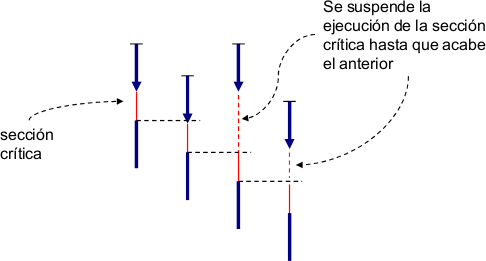
\includegraphics[width=0.8\textwidth]{./img/gnuplot/secc_crit.png}
\caption{\label{PROC_secc_crit}Sincronización: La exclusión de las \emph{secciones críticas} entre a varios procesos se protegen por medio de regiones de \emph{exclusión mutua}}
\end{figure}

Hay que tener en cuenta que un mutex \emph{no implica} que el código no se
va a interrumpir mientras se está dentro de esta región — Eso sería
muy peligroso, dado que permitiría que el sistema operativo pierda el
control del planificador, volviendo (para propósitos prácticos) a un
esquema de multitarea cooperativa. El mutex es un \emph{mecanismo de prevención}, que mantiene en espera a cualquier hilo o proceso que
quiera entrar a la \emph{sección crítica} protegida por el mutex,
 reteniéndolo antes de entrar a
ésta hasta que el proceso que la está
ejecutando salga de ella. Si no hay ningún hilo o proceso en dicha
sección crítica (o cuando un hilo sale de ella), uno
sólo de los que esperan podrá ingresar.

Como se vio en el ejemplo anterior, para que un mutex sea efectivo
tiene que ser implementado a través de una \emph{primitiva} a un nivel
inferior\footnote{¿Qué significa inferior? Las llamadas de sincronización
entre hilos deben implementarse por lo menos a nivel del proceso que
los contiene; aquellas que se realizan entre procesos independientes,
deben implementarse a nivel del sistema operativo. Debe haber un
agente \emph{más abajo} en niveles de abstracción, en control \emph{real} del
equipo de cómputo, ofreciendo estas operaciones. }, implicando al
planificador.

El problema de la actualización múltiple que surge en el caso de la
venta de pasajes aereos podría reescribirse de la siguiente manera
empleando un mutex:


\begin{verbatim}
my ($proximo_asiento :shared, $capacidad :shared);
$capacidad = 40;

sub asigna_asiento {
  lock($proximo_asiento);
  if ($proximo_asiento < $capacidad) {
    $asignado = $proximo_asiento;
    $proximo_asiento += 1;
    print "Asiento asignado: $asignado\n";
  } else {
    print "No hay asientos disponibles\n";
    return 1;
  }
  return 0;
}
\end{verbatim}

Se debe tener en cuenta que en este caso se utiliza una implementación
de hilos, esto hace que la solución sea dependiente del lenguaje
específico de implementación, en este caso Perl. Al ser
\texttt{\$proximo\_asiento} una variable compartida tiene algunas \emph{propiedades}
adicionales, en este caso, la de poder operar como un mutex. La
implementación en Perl resulta muy \emph{limpia}, dado que evita el uso
de un candado explícito — Se podría leer la línea 5 como \emph{exclusión mutua sobre} \texttt{\$proximo\_asiento}.

En la implementación de hilos de Perl, la función \texttt{lock()} implementa
un mutex delimitado por el \emph{ámbito léxico} de su invocación: el área
de exclusión mutua abarca desde la línea 5 en que es invocada hasta la
15 en que termina el bloque en que se invocó.

Un área de exclusion mutua debe:

\begin{description}
\item[Ser mínima] Debe ser \emph{tan corta como sea posible}, para evitar que
                otros hilos queden bloqueados fuera del área
                crítica. Si bien en este ejemplo es demasiado simple,
                si se hiciera cualquier llamada a otra función (o al
                sistema) estando dentro de un área de exclusión mutua,
                se detendría la ejecución de todos los demás hilos por
                mucho más tiempo del necesario.
\item[Ser completa] Se debe analizar bien cuál es el área a
     proteger y no arriesgarse a proteger de menos. En este ejemplo,
     se podría haber puesto \texttt{lock(\$asignado)} dentro del \texttt{if}, dado
     que sólo dentro de su evaluación positiva se modifica la variable
     \texttt{\$proximo\_asiento}. Sin embargo, si la ejecución de un hilo se
     interrumpiera entre las líneas 7 y 8, la condición del \texttt{if} se
     podría evaluar incorrectamente.
\end{description}

Como comparación, una rutina equivalente en Bash (entre procesos
independientes y usando los archivos \texttt{/tmp/proximo\_asiento} y
\texttt{/etc/capacidad/} como un mecanismo para compartir datos) sería:


\begin{verbatim}
asigna_asiento() {
  lockfile /tmp/asigna_asiento.lock
  PROX=$(cat /tmp/proximo_asiento || echo 0)
  CAP=$(cat /etc/capacidad || echo 40)
  if [ $PROX -lt $CAP ]
    then
      ASIG=$PROX
      echo $(($PROX+1)) > /tmp/proximo_asiento
      echo "Asiento asignado: $ASIG"
    else
      echo "No hay asientos disponibles"
      return 1;
    fi
  rm -f /tmp/asigna_asiento.lock
}
\end{verbatim}

Cabe mencionar que \texttt{lockfile} no es una función implementada en Bash,
sino que envuelve a una \emph{llamada al sistema}. El sistema operativo
garantiza que la verificación y creación de este \emph{candado} se
efectuará de forma atómica.

Un mutex es, pues, una herramienta muy sencilla, y podría verse como
la pieza básica para la sincronización entre procesos. Lo fundamental
para emplearlos es identificar las regiones críticas del código, y
proteger el acceso \emph{con un mecanismo apto de sincronización}, que
garantice atomicidad.
\subsubsection{Semáforos}
\label{sec-3-3-3-2}


La interfaz ofrecida por los mutexes es muy sencilla, pero no permite
resolver algunos problemas de sincronización. Edsger Dijkstra, en
1968, propuso los \emph{semáforos}.\footnote{El símil presentado por Dijkstra
no es del semáforo vial, con una luz roja y una luz verde (dicho
esquema se asemeja al del \emph{mutex}). La referencia es a la del semáforo
de tren, que permite el paso estando \emph{arriba}, e indica espera estando
\emph{abajo}. } 

Un semáforo es una variable de tipo entero que tiene definida la
siguiente interfaz:

\begin{description}
\item[Inicialización] Se puede inicializar el semáforo a cualquier valor
                    entero, pero después de esto, su valor no puede ya
                    ser leído. Un semáforo es una \emph{estructura                     abstracta}, y su valor es tomado como \emph{opaco}
                    (invisible) al programador.
\item[Decrementar] Cuando un hilo decrementa el semáforo, si el valor es
                 negativo, el hilo se \emph{bloquea} y no puede continuar
                 hasta que \emph{otro hilo} incremente el semáforo. Según
                 la implementación, esta operación puede denominarse
                 \texttt{wait}, \texttt{down}, \texttt{acquire} o incluso \texttt{P} (por ser la
                 inicial de \emph{proberen te verlagen}, \emph{intentar                  decrementar} en holandés, del planteamiento original
                 en el artículo de Dijkstra).
\item[Incrementar] Cuando un hilo incrementa el semáforo, si hay hilos
                 esperando, uno de ellos es \emph{despertado}. Los nombres
                 que recibe esta operación son \texttt{signal}, \texttt{up},
                 \texttt{release}, \texttt{post} o \texttt{V} (de \emph{verhogen},
                 \emph{incrementar}).
\end{description}

La interfaz de hilos \texttt{POSIX} (\texttt{pthreads}) presenta esas primitivas
con la siguiente definición:


\begin{verbatim}
int sem_init(sem_t *sem, int pshared, unsigned int value);
int sem_post(sem_t *sem);
int sem_wait(sem_t *sem);
int sem_trywait(sem_t *sem);
\end{verbatim}

La variable \texttt{pshared} indica si el semáforo puede ser compartido
entre procesos o únicamente entre hilos. \texttt{sem\_trywait} extiende la
intefaz sugerida por Dijkstra: verifica si el semáforo puede ser
decrementado y, en caso de que no, en vez de bloquearse, indica al
proceso que no puede continuar. El proceso debe tener la lógica
necesaria para no entrar en las secciones críticas (p. ej., intentar
otra estrategia) en ese caso.

\texttt{sem\_trywait} se sale de la definición clásica de semáforo, por lo
que no se considera en esta sección.

Un semáforo permite la implementación de varios patrones, entre los
cuales se mencionarán los siguientes:

\begin{description}
\item[Señalizar] Un hilo debe informar a otro que cierta condición está
               ya cumplida — Por ejemplo, un hilo prepara una conexión
               en red mientras que otro calcula lo que tiene que
               enviar. No se puede arriesgar a comenzar a enviar
               antes de que la conexión esté lista. Se inicializa el
               semáforo a 0, y:


\begin{verbatim}
# Antes de lanzar los hilos
senal = Semaphore(0)

def envia_datos():
  calcula_datos()
  senal.acquire()
  envia_por_red()

def prepara_conexion():
  crea_conexion()
  senal.release()
\end{verbatim}
\end{description}

	       No importa si \texttt{prepara\_conexion()} termina primero — En
	       el momento en que termine, \texttt{senal} valdrá 1 y
	       \texttt{envia\_datos()} podrá proceder.

\begin{description}
\item[\emph{Rendezvous}] Así se denomina en francés (y ha sido adoptado al
                  inglés) a quedar en una \emph{cita}. Este patrón busca
                  que dos hilos se esperen mutuamente en cierto punto
                  para continuar en conjunto — Por ejemplo, en una
                  aplicación GUI, un hilo prepara la interfaz gráfica
                  y actualiza sus eventos mientras otro efectúa
                  cálculos para mostrar. Se desea presentar al usuario
                  la simulación desde el principio, así que no debe
                  empezar a calcular antes de que el GUI esté listo,
                  pero preparar los datos del cálculo toma tiempo, y
                  no se quiere esperar doblemente. Para esto, se
                  implementan dos semáforos señalizándose mutuamente:


\begin{verbatim}
guiListo = Semaphore(0)
calculoListo = Semaphore(0)

threading.Thread(target=maneja_gui, args=[]).start()
threading.Thread(target=maneja_calculo, args=[]).start()

def maneja_gui():
  inicializa_gui()
  guiListo.release()
  calculoListo.acquire()
  recibe_eventos()

def maneja_calculo():
  inicializa_datos()
  calculoListo.release()
  guiListo.acquire()
  procesa_calculo()
\end{verbatim}
\end{description}

\begin{description}
\item[Mutex] El uso de un semáforo inicializado a 1 puede implementar
	   fácilmente un mutex. En Python:


\begin{verbatim}
mutex = Semaphore(1)
# ...Inicializar estado y lanzar hilos
mutex.acquire()
#  Aquí se está en la region de exclusión mutua
x = x + 1
mutex.release()
# Continúa la ejecucion paralela
\end{verbatim}
\end{description}

\begin{description}
\item[Multiplex] Permite la entrada de no más de \emph{n} procesos a la
               región crítica. Si se lo ve como una generalización de
               \emph{Mutex}, basta con inicializar al semáforo al número
               máximo de procesos deseado.

	       Su construcción es idéntica a la de un mutex, pero es
               inicializado al número de procesos que se quiere
               permitir que ejecuten de forma simultánea.
\item[Torniquete] Una construcción que por sí sóla no hace mucho, pero
                resulta útil para patrones posteriores. Esta
                construcción garantiza que un grupo de hilos o
                procesos \emph{pasa por un punto determinado} de uno en uno
                (incluso en un ambiente multiprocesador):


\begin{verbatim}
torniquete = Semaphore(0)
# (...)
if alguna_condicion():
  torniquete.release()
# (...)
torniquete.acquire()
torniquete.release()
\end{verbatim}
\end{description}

                En este caso, se ve primero una \emph{señalización} que
                hace que todos los procesos esperen frente al
                torniquete hasta que alguno marque que
                \texttt{alguna\_condicion()} se ha cumplido y libere el
                paso. Posteriormente, los procesos que esperan
                pasarán ordenadamente por el torniquete.

		El torniquete por sí sólo no es tan útil, pero su
                función se hará clara a continuación.

\begin{description}
\item[Apagador] Cuando se tiene una situación de \emph{exclusión categórica}
              (basada en categorías y no en procesos individuales —
              Varios procesos de la misma categoría pueden entrar a la
              sección crítica, pero procesos de dos categorías
              distintas deben tenerlo prohibido), un \emph{apagador}
              permite evitar la inanición de una de las categorías
              ante un flujo constante de procesos de la otra.

	      El apagador usa, como uno de sus componentes, a un
	      torniquete. Para ver una implementación ejemplo de un
	      apagador, referirse a la solución presentado a
	      continuación para el problema lectores-escritores.
\item[Barrera] Una barrera es una generalización de \emph{rendezvous} que
             permite la sincronización entre varios hilos (no sólo
             dos), y no requiere que el rol de cada uno de los hilos
             sea distinto.

	     Esta construcción busca que ninguno de los hilos
             continúe ejecutando hasta que todos hayan llegado a un
             punto dado.

	     Para implementar una barrera, es necesario que ésta
             guarde algo de información adicional además del semáforo,
             particularmente, el número de hilos que se han lanzado
             (para esperarlos a todos). Esta será una variable
             compartida y, por tanto, requiere de un mutex. La
             inicialización (que se ejecuta antes de iniciar los
             hilos) será:


\begin{verbatim}
require random
n = random.randint(1,10) # Número de hilos
cuenta = 0
mutex = Semaphore(1)
barrera = Semaphore(0)
\end{verbatim}
\end{description}

	     Ahora, suponiendo que todos los hilos tienen que
             realizar, por separado, la inicialización de su estado,
             y ninguno de ellos debe comenzar el procesamiento hasta
             que todos hayan efectuado su inicialización:


\begin{verbatim}
inicializa_estado()

mutex.acquire()
cuenta = cuenta + 1
mutex.release()

if cuenta == n:
  barrera.release()

barrera.acquire()
barrera.release()

procesamiento()
\end{verbatim}

	     Las barreras son una construcción suficientemente útil
             como para que sea común encontrarlas ``prefabricadas''. En
             los hilos \texttt{POSIX} (\texttt{pthreads}), por ejemplo, la interfaz
             básica es:


\begin{verbatim}
int pthread_barrier_init(pthread_barrier_t  *barrier,
                         const pthread_barrierattr_t *restrict attr,
                         unsigned count);
int pthread_barrier_wait(pthread_barrier_t  *barrier);
int pthread_barrier_destroy(pthread_barrier_t *barrier);
\end{verbatim}

\begin{description}
\item[Cola] Se emplea una cola cuando se tienen dos \emph{clases de}
          hilos que deben proceder en pares. Este patrón es a veces
          referido como \emph{baile de salón}: para que una pareja baile,
          hace falta que haya un \emph{líder} y un \emph{seguidor}. Cuando
          llega una persona al salón, verifica si hay uno de la otra
          clase esperando bailar. En caso de haberlo, bailan, y en
          caso contrario, espera a que llegue su contraparte.

	  El código para implementar esto es muy simple:


\begin{verbatim}
colaLideres = Semaphore(0)
colaSeguidores = Semaphore(0)
# (...)
def lider():
  colaSeguidores.release()
  colaLideres.acquire()
  baila()
def seguidor():
  colaLideres.release()
  colaSeguidores.acquire()
  baila()
\end{verbatim}
\end{description}

	  El patrón debe resultar ya familiar: es un \emph{rendezvous}. La
          distinción es meramente semántica: en el \emph{rendezvous}
          se necesitan dos hilos explícitamente, aquí se habla de
          dos clases de hilos.

	  Sobre este patrón base se pueden refinar muchos
          comportamientos. Por ejemplo, asegurar que sólo una pareja
          esté bailando al mismo tiempo, o asegurar que los hilos en
          espera vayan bailando en el orden en que llegaron.
ORG-LIST-END-MARKER
\subsubsection{Variables de condición}
\label{sec-3-3-3-3}


Las variables de condición presentan una extensión sobre el
comportamiento de los mutexes, buscando darles la ``inteligencia'' de
responder ante determinados eventos. Una variable de condición siempre
opera \emph{en conjunto con} un mutex, y en algunas implementaciones es
necesario indicar cuál será dicho mutex desde la misma inicialización
del objeto.\footnote{Mientras que otras implementaciones permiten que se
declaren por separado, pero siempre que se invoca a una variable
de condición, debe indicársele qué mutex estará empleando. }

Una variable de condición presenta las siguientes operaciones:

\begin{description}
\item[Espera] Se le indica una condición y un mutex. El mutex tiene que
            haber sido ya adquirido. Esta operación \emph{libera} al mutex,
            y se bloquea hasta recibir una \emph{notificación} de otro hilo
            o proceso. Una vez que la notificación es recibida, y
            antes de devolver la ejecución al hilo, \emph{re-adquiere} el
            mutex.
\item[Espera medida] Tiene una semántica igual a la de la espera, pero
                   recibe un argumento adicional, indicando el tiempo
                   de expiración. Si pasado el tiempo de expiración
                   no ha sido notificado, despierta al hilo
                   regresándole un error (y sin re-adquirir el
                   mutex).
\item[Señaliza] Requiere que el mutex ya haya sido adquirido. Despierta
              (señaliza) a uno o más hilos (algunas implementaciones
              permiten indicar como argumento a cuántos hilos) de los
              que están bloqueados en la espera asociada. \emph{No} libera
              el mutex — Esto significa que el flujo de ejecución \emph{se               mantiene en el invocante}, quien tiene que salir de su
              sección crítica (entregar el mutex) antes de que otro de
              los hilos continúe ejecutando.
\item[Señaliza a todos] Indica a \emph{todos los hilos} que estén esperando a
     esta condición.
\end{description}

La interfaz de hilos \texttt{POSIX} (\texttt{pthreads}) presenta la siguiente
definición:


\begin{verbatim}
pthread_cond_t cond = PTHREAD_COND_INITIALIZER;
int pthread_cond_init(pthread_cond_t *cond, pthread_condattr_t *cond_attr);
int pthread_cond_signal(pthread_cond_t *cond);
int pthread_cond_broadcast(pthread_cond_t *cond);
int pthread_cond_wait(pthread_cond_t *cond, pthread_mutex_t *mutex);
int pthread_cond_timedwait(pthread_cond_t *cond, pthread_mutex_t *mutex, const struct timespec *abstime);
int pthread_cond_destroy(pthread_cond_t *cond);
\end{verbatim}
\subsection{Problema productor-consumidor}
\label{sec-3-3-4}
\subsubsection{Planteamiento}
\label{sec-3-3-4-1}

En un entorno multihilos es común que haya una división de tareas tipo
\emph{línea de ensamblado}, que se puede generalizar a que un grupo de
hilos van \emph{produciendo} ciertas estructuras, a ser \emph{consumidas} por
otro grupo.

Un ejemplo de este problema puede ser un programa \emph{orientado a eventos}, en que eventos de distinta naturaleza pueden producirse, y
causan que se \emph{disparen} los mecanismos que los puedan atender. Los
eventos pueden \emph{apilarse} en un buffer que será procesado por los
hilos encargados conforme se vayan liberando. Esto impone ciertos
requisitos, como:

\begin{itemize}
\item Debido a que el buffer es un recurso compartido por los hilos,
	agregar o retirar un elemento del buffer tiene que ser hecho de
       forma atómica. Si más de un proceso intentara hacerlo al mismo
       tiempo, se correría el riesgo de que se corrompan los datos.
\item Si un consumidor está listo y el buffer está vacío, debe
       bloquearse (¡no realizar espera activa!) hasta que un productor
       genere un elemento.
\end{itemize}

  Si no se tiene en cuenta la sincronización, el código sería tan
  simple como el siguiente:


\begin{verbatim}
import threading
buffer = []
threading.Thread(target=productor,args=[]).start()
threading.Thread(target=consumidor,args=[]).start()

def productor():
  while True:
    event = genera_evento()
    buffer.append(event)

def consumidor():
  while True:
    event = buffer.pop()
    procesa(event)
\end{verbatim}

  Pero el acceso a \texttt{buffer} no está protegido para garantizar la
  exclusión mutua, y podría quedar en un estado inconsistente si
  \texttt{append()} y \texttt{pop()} intentan manipular sus estructuras al mismo
  tiempo. Además, si bien en este ejemplo se asumió que hay un sólo hilo
  productor y un sólo hilo consumidor, se puede extender el programa
  para que haya varios hilos en cualquiera de estos roles.

  \texttt{evento} no requiere de protección, dado que es una variable local a
  cada hilo.
\subsubsection{Solución}
\label{sec-3-3-4-2}

   Para resolver este problema se usarán dos semáforos: \texttt{mutex}, que
   protege el acceso a la sección crítica, y \texttt{elementos}. El valor
   almacenado en \texttt{elementos} indica, cuando es positivo, cuántos
   eventos pendientes hay por procesar, y cuando es negativo, cuántos
   consumidores están listos y esperando un evento.

   Una solución a este problema puede ser:


\begin{verbatim}
import threading
mutex = threading.Semaphore(1)
elementos = threading.Semaphore(0)
buffer = []
threading.Thread(target=productor, args=[]).start()
threading.Thread(target=consumidor, args=[]).start()

def productor():
  while True:
    event = genera_evento()
    mutex.acquire()
    buffer.append(event)
    mutex.release()
    elementos.release()

def consumidor():
  while True:
    elementos.acquire()
    mutex.acquire()
    event = buffer.pop()
    mutex.release()
    event.process()
\end{verbatim}

   Se puede ver que la misma construcción, un semáforo, es utilizada de
   forma muy distinta por \texttt{mutex} y \texttt{elementos}. \texttt{mutex} implementa una
   exclusión mutua clásica, delimitando tanto como es posible (a una
   sóla línea en este caso) al área crítica, y siempre apareando un
   \texttt{acquire()} con un \texttt{release()}. \texttt{elementos}, en cambio, es empleado
   como un verdadero semáforo: como una estructura para la
   sincronización. Sólo los hilos productores incrementan (sueltan) el
   semáforo, y sólo los consumidores lo decrementan (adquieren). Esto
   es, ambos semáforos comunican \emph{al planificador} cuándo es posible
   despertar a algún consumidor.

   Si se supone que \texttt{genera\_evento()} es eficiente y no utiliza 
   espera activa, esta implementación es óptima: deja en manos
   del planificador toda la espera necesaria, y no desperdicia recursos
   de cómputo esperando a que el siguiente elemento esté listo.

   Como nota al pie, la semántica del módulo \texttt{threading} de Python
   incluye la declaración de contexto \texttt{with}. Todo objeto de
   \texttt{threading} que implemente \texttt{acquire()} y \texttt{release()} puede ser
   envuelto en un bloque \texttt{with}, aumentando la legibilidad y con
   exactamente la misma semántica; no se utilizó en este ejemplo para
   ilustrar el uso tradicional de los semáforos para implementar
   regiones de exclusión mutua, sin embargo y sólo para concluir con el
   ejemplo, la función \texttt{consumidor()} final podría escribirse así, y
   ser semánticamente idéntica:


\begin{verbatim}
def consumidor():
  while True:
    elementos.acquire()
    with mutex:
      event = buffer.pop()
    event.process()
\end{verbatim}

   A pesar de ser más clara, no se empleará en este texto esta notación
   por dos razones. La primera es para mantener la conciencia de la
   semántica de las operaciones \texttt{acquire()} y \texttt{release()}, y la segunda
   es mantener la consistencia a través de las distintas
   implementaciones, ya que se encontrarán varios casos en que no es el
   mismo hilo el que adquiere un semáforo y el que lo libera (esto es,
   los semáforos no siempre son empleados como mutexes).
\subsection{Bloqueos mutuos e inanición}
\label{sec-3-3-5}


Cuando hay concurrencia, además de asegurar la atomicidad de ciertas
operaciones, se debe evitar dos problemas que son consecuencia natural
de la existencia de la asignación de recursos de forma exclusiva:

\begin{description}
\item[Bloqueo mutuo] (o \emph{interbloqueo}; en inglés, \emph{deadlock}) Situación
                   que ocurre cuando dos o más procesos poseen
                   determinados recursos, y cada uno queda detenido, a
                   la espera de alguno de los que tiene el otro. El
                   sistema puede seguir operando normalmente, pero
                   ninguno de los procesos involucrados podrán
                   avanzar.
\item[Inanición] (en inglés \emph{resource starvation}) Situación en que un
	       proceso no puede avanzar en su ejecución dado que necesita
	       recursos que están (alternativamente) asignados a
	       otros procesos.
\end{description}

El que se presenten estos conceptos aquí no significa que están
\emph{exclusivamente} relacionados con este tema: son conceptos que
se enfrentan una y otra vez al hablar de asignación exclusiva de
recursos — temática recurrente en el campo de los sistemas operativos.
\subsection{Problema lectores-escritores}
\label{sec-3-3-6}
\subsubsection{Planteamiento}
\label{sec-3-3-6-1}

      Una estructura de datos puede ser accedida simultáneamente por
      muchos procesos \emph{lectores}, pero si algún proceso está
      escribiendo, se debe evitar que cualquier otro lea (dado que
      podría encontrarse con los datos en un estado inconsistente). Los
      requisitos de sincronización son

\begin{itemize}
\item Cualquier cantidad de lectores puede estar leyendo al mismo
       	tiempo.
\item Los escritores deben tener acceso exclusivo a la sección
       	crítica.
\item En pos de un comportamiento más justo: se debe evitar que un
       	influjo constante de procesos lectores dejen a un escritor en
       	situación de \emph{inanición}.
\end{itemize}
\subsubsection{Discusión}
\label{sec-3-3-6-2}


   Este problema puede ser generalizado como una \emph{exclusión mutua    categórica}: se debe separar el uso de un recurso según la categoría
   del proceso. La presencia de un proceso en la sección crítica no
   lleva a la exclusión de otros, pero sí hay \emph{categorías} de procesos
   que tienen distintas reglas — Para los escritores \emph{sí} hace falta
   una exclusión mutua completa.
\subsubsection{Primera aproximación}
\label{sec-3-3-6-3}

   Un primer acercamiento a este problema permite una resolución
   libre de bloqueos mutuos, empleando sólo tres estructuras globales:
   un contador que indica cuántos lectores hay en la sección crítica,
   un mutex protegiendo a dicho contador, y otro mutex indicando que no
   hay lectores ni escritores accediendo al buffer (o
   cuarto). Se implementan los mutexes con semáforos. 


\begin{verbatim}
import threading
lectores = 0
mutex = threading.Semaphore(1)
cuarto_vacio = threading.Semaphore(1)

def escritor():
  cuarto_vacio.acquire()
  escribe()
  cuarto_vacio.release()

def lector():
  mutex.acquire()
  lectores = lectores + 1
  if lectores == 1:
    cuarto_vacio.acquire()
  mutex.release()

  lee()

  mutex.acquire()
  lectores = lectores - 1
  if lectores == 0:
    cuarto_vacio.release()
  mutex.release()
\end{verbatim}

   El semáforo \texttt{cuarto\_vacio} sigue un patrón visto antes llamado \emph{apagador}. El
   escritor utiliza al apagador como a cualquier mutex: lo utiliza para
   rodear a su sección crítica. El lector, sin embargo, lo emplea de
   otra manera. Lo primero que hace es verificar \emph{si la luz está    prendida}, esto es, si hay algún otro lector en el cuarto (si
   \texttt{lectores} es igual a 1). Si es el primer lector en entrar, prende
   la luz adquiriendo \texttt{cuarto\_vacio} (lo cual evitará que un escritor
   entre). Cualquier cantidad de lectores puede entrar, actualizando su
   número. Cuando el último sale (\texttt{lectores} es igual a 0), apaga la
   luz.

   El problema con esta implementación es que un flujo constante de
   lectores puede llevar a la inanición de un escritor, que está
   pacientemente parado esperando a que alguien apague la luz.
\subsubsection{Solución}
\label{sec-3-3-6-4}


   Para evitar esta condición de inanición, se puede agregar un
   \emph{torniquete} evitando que lectores adicionales se \emph{cuelen} antes del
   escritor. Reescribiendo:


\begin{verbatim}
import threading
lectores = 0
mutex = threading.Semaphore(1)
cuarto_vacio = threading.Semaphore(1)
torniquete = threading.Semaphore(1)

def escritor():
  torniquete.acquire()
  cuarto_vacio.acquire()
  escribe()
  cuarto_vacio.release()
  torniquete.release()

def lector():
  global lectores
  torniquete.acquire()
  torniquete.release()

  mutex.acquire()
  lectores = lectores + 1
  if lectores == 1:
    cuarto_vacio.acquire()
  mutex.release()

  lee()

  mutex.acquire()
  lectores = lectores - 1
  if lectores == 0:
    cuarto_vacio.release()
  mutex.release()
\end{verbatim}

   En la implementación de los escritores, esto puede parecer inútil:
   Únicamente se agregó un mutex redundante alrededor de lo que ya
   se tenía. Sin embargo, al obligar a que el lector pase por un
   torniquete antes de actualizar \texttt{lectores}, lo cual obligaría a que
   se mantenga encendida la luz, se obliga a que espere a que el
   escritor suelte este mutex exterior. Nuevamente se puede ver cómo la misma
   estructura es tratada de dos diferentes maneras: para el lector es
   un torniquete, y para el escritor es un mutex.
\subsection{La cena de los filósofos}
\label{sec-3-3-7}
\subsubsection{Planteamiento}
\label{sec-3-3-7-1}

      Cinco filósofos se dan cita para comer arroz en una mesa
      redonda. En la mesa, cada uno de ellos se sienta frente a un
      plato. A su derecha, tiene un palito chino, y a su izquierda
      tiene otro.

      Los filósofos sólo saben \texttt{pensar()} y \texttt{comer()}. Cada uno de
      ellos va a \texttt{pensar()} un tiempo arbitrario, hasta que le da
      hambre. El hambre es mala consejera, por lo que intenta
      \texttt{comer()}. Los requisitos son:

\begin{itemize}
\item Sólo un filósofo puede sostener determinado palito a la vez, esto es
       	los palitos son recursos de acceso exclusivo.
\item Debe ser imposible que un filósofo muera de inanición estando a
       	la espera de un palito.
\item Debe ser imposible que se presente un bloqueo mutuo.
\item Debe ser posible que más de un filósofo pueda comer al mismo
       	tiempo.
\end{itemize}
\subsubsection{Discusión}
\label{sec-3-3-7-2}

   En este caso, el peligro no es, como en el ejemplo anterior, que una
   estructura de datos sea sobreescrita por ser accedida por dos hilos
   al mismo tiempo, sino que se presenten situaciones en el curso normal de
   la operación que lleven a un bloqueo mutuo.

   A diferencia del caso antes descripto, ahora se utilizarán los
   semáforos no como una herramienta para indicar al planificador
   cuándo despertar a uno de los hilos, sino como una herramienta de
   comunicación entre los propios hilos.
\subsubsection{Primer acercamiento}
\label{sec-3-3-7-3}


   Se puede representar a los palillos como un arreglo de semáforos,
   asegurando la exclusión mutua (esto es, sólo un filósofo puede
   sostener un palillo al mismo tiempo), pero eso no evita el bloqueo
   mutuo. Por ejemplo, si la  solución fuera:


\begin{verbatim}
import threading
num = 5
palillos = [threading.Semaphore(1) for i in range(num)]
filosofos = [threading.Thread(target=filosofo, args=[i]).start() for i in range(num)]

def filosofo(id):
  while True:
    piensa(id)
    levanta_palillos(id)
    come(id)
    suelta_palillos(id)

def piensa(id):
  # (...)
  print "%d - Tengo hambre..." % id

def levanta_palillos(id):
  palillos[(id+1) % num].acquire()
  print "%d - Tengo el palillo derecho" % id
  palillos[id].acquire()
  print "%d - Tengo ambos palillos" % id

def suelta_palillos(id):
  palillos[(id+1) % num].release()
  palillos[id].release()
  print "%d - Sigamos pensando..." % id

def come(id):
  print "%d - ¡A comer!" % id
  # (...)
\end{verbatim}

   Podría pasar que todos los filósofos quieran comer al mismo tiempo,
   y el planificador dejara suspendidos a todos con el palillo derecho
   en la mano.
\subsubsection{Solución}
\label{sec-3-3-7-4}


   Ahora, ¿qué pasa si se hace que algunos filósofos sean \emph{zurdos}?
   Esto es, que levanten primero el palillo izquierdo y luego el
   derecho:


\begin{verbatim}
def levanta_palillos(id):
  if (id % 2 == 0): # Zurdo
    palillo1 = palillos[id]
    palillo2 = palillos[(id+1) % num]
  else: # Diestro
    palillo1 = paltos[(id+1) % num]
    palillo2 = palillos[id]
  palillo1.acquire()
  print "%d - Tengo el primer palillo" % id
  palillo2.acquire()
  print "%d - Tengo ambos palillos" % id
\end{verbatim}

   Al asegurar que dos filósofos contiguos no intenten levantar el
   mismo palillo, se tiene la certeza de que no se producirán bloqueos
   mutuos. De hecho, incluso si sólo uno de los filósofos es zurdo,
   se puede demostrar que no habrá bloqueos:


\begin{verbatim}
def levanta_palillos(id):
  if id == 0: # Zurdo
    palillos[id].acquire()
    print "%d - Tengo el palillo izquierdo" % id
    palillos[(id+1) % num].acquire()
  else: # Diestro
    palillos[(id+1) % num].acquire()
    print "%d - Tengo el palillo derecho" % id
    palillos[id].acquire()
  print "%d - Tengo ambos palillos" % id
\end{verbatim}

   Cabe apuntar que ninguno de estos mecanismos asegura que en la mesa
   no haya \emph{inanición}, sólo que no haya bloqueos mutuos.
\subsection{Los fumadores compulsivos}
\label{sec-3-3-8}
\subsubsection{Planteamiento}
\label{sec-3-3-8-1}

Hay tres fumadores empedernidos y un \emph{agente} que, de tiempo en
     tiempo, consigue ciertos insumos. Los ingredientes necesarios
     para fumar son tabaco, papel y cerillos. Cada uno de los
     fumadores tiene una cantidad infinita de alguno de los
     ingredientes, pero no les gusta compartir. Afortunadamente, del
     mismo modo que no comparten, no son acaparadores\footnote{Esto es, no
     buscan obtener y conservar los recursos \emph{preventivamente}, sino
     que los toman sólo cuando satisfacen \emph{por completo} sus
     necesidades. }.

     De tiempo en tiempo, el agente consigue una dosis de dos de los
     ingredientes — Por ejemplo, si deja en la mesa un papel y tabaco,
     el que trae los cerillos educadamente tomará los ingredientes, se
     hará un cigarro, y lo fumará.

     Suhas Patil (1971) planteó este problema buscando demostrar que
     hay situaciones que no se pueden resolver con el uso de
     semáforos. Las condiciones planteadas son

\begin{itemize}
\item No se puede  modificar el código del agente. Si el agente es un
       sistema operativo, ¡tiene sentido la restricción de no tenerle
       que notificar acerca de los flujos a cada uno de los programas
       que ejecuta!
\item El planteamiento original de Patil menciona que no debe
       emplearse arreglos de semáforos o usar condicionales en el
       flujo. Esta segunda restricción haría efectivamente irresoluble
       al problema, por lo que se ignorará.
\end{itemize}
\subsubsection{Primer acercamiento}
\label{sec-3-3-8-2}


Al haber tres distintos ingredientes, tiene sentido que se empleen tres
distintos semáforos, para señalizar a los fumadores respecto a cada
uno de los ingredientes. Un primer acercamiento podría ser:


\begin{verbatim}
import random
import threading
ingredientes = ['tabaco', 'papel', 'cerillo']
semaforos = {}
semaforo_agente = threading.Semaphore(1)
for i in ingredientes:
  semaforos[i] = threading.Semaphore(0)

threading.Thread(target=agente, args=[]).start()
fumadores = [threading.Thread(target=fumador, args=[i]).start() for i in ingredientes]

def agente():
  while True:
    semaforo_agente.acquire()
    mis_ingr = ingredientes[:]
    mis_ingr.remove(random.choice(mis_ingr))
    for i in mis_ingr:
      print "Proveyendo %s" % i
      semaforos[i].release()

def fumador(ingr):
  mis_semaf = []
  for i in semaforos.keys():
    if i != ingr:
      mis_semaf.append(semaforos[i])
  while True:
    for i in mis_semaf:
      i.acquire()
    fuma(ingr)
    semaforo_agente.release()

def fuma(ingr):
  print 'Fumador con %s echando humo...' % ingr
\end{verbatim}

El problema en este caso es que, al tener que cubrir un número de
ingredientes mayor a uno, utilizar sólo un semáforo ya no funciona: si
\texttt{agente()} decide proveer papel y cerillos, nada garantiza que no sea
el \texttt{fumador['cerillo']} el que reciba la primer señal o que
\texttt{fumador['tabaco']} reciba la segunda — Para que este programa avance
hace falta, más que otra cosa, la buena suerte de que las señales sean
recibidas por el proceso indicado.
\subsubsection{Solución}
\label{sec-3-3-8-3}


Una manera de evitar esta situación es la utilización de
\emph{intermediarios} encargados de notificar al hilo adecuado. Partiendo
de que, respetando la primer restricción impuesta por Patil, no
se puede modificar el código del agente, se implementan los
intermediarios, se reimplementan los fumadores y se agregan algunas
variables globales, de esta manera:


\begin{verbatim}
que_tengo = {}
semaforos_interm = {}
for i in ingredientes:
  que_tengo[i] = False
  semaforos_interm[i] = threading.Semaphore(0)
interm_mutex = threading.Semaphore(1)
intermediarios = [threading.Thread(target=intermediario, args=[i]).start() for i in ingredientes]

def fumador(ingr):
  while True:
    semaforos_interm[ingr].acquire()
    fuma(ingr)
    semaforo_agente.release()

def intermediario(ingr):
  otros_ingr = ingredientes[:]
  otros_ingr.remove(ingr)
  while True:
    semaforos[ingr].acquire()
    interm_mutex.acquire()
    for i in otros_ingr:
      if que_tengo[i]:
        que_tengo[i] = False
        semaforos_interm[i].release()
        break
      que_tengo[i] = True
    interm_mutex.release()
\end{verbatim}

Si bien se ve que el código de \texttt{fumador()} se simplifica (dado que ya
no tiene que efectuar ninguna verificación), \texttt{intermediario()} tiene
mayor complejidad. El elemento clave de su lógica es que, si bien el
\texttt{agente()} (el sistema operativo) seguirá enviando una señal por
cada ingrediente disponible, los tres intermediarios se sincronizarán
empleando al arreglo \texttt{que\_tengo} (protegido por \texttt{interm\_mutex}), y de
este modo cada hilo (independientemente del orden en que fue invocado)
señalizará a los otros intermediarios qué ingredientes hay en la mesa,
y una vez que sepa a qué fumador notificar, dejará el estado listo
para recibir una nueva notificación.
\subsection{Otros mecanismos}
\label{sec-3-3-9}


Más allá de los mecanismos basados en mutexes y semáforos, existen
otros que emplean diferentes niveles de \emph{encapsulamiento}
para proteger las abstracciones. A continuación se presentan muy
brevemente algunos de ellos.
\subsubsection{Monitores}
\label{sec-3-3-9-1}


El principal problema con los mecanismos anteriormente descritos es
que no sólo hace falta encontrar un mecanismo que permita evitar el
acceso simultáneo a la sección crítica sin caer en bloqueos mutuos o
inanición, sino que hay que \emph{implementarlo correctamente}, empleando
una semántica que requiere de bastante entrenamiento para entender
correctamente.

Además, al hablar de procesos que compiten por recursos de una forma
\emph{hostil}, la implementación basada en semáforos puede resultar
insuficiente. A mode de ejemplo, se mostrará por qué en el modelo
original de Djikstra (así como en los ejemplos presentados
anteriormente) sólo existen las operaciones de incrementar y
decrementar, y no se permite verificar el estado (como lo ofrece
\texttt{sem\_trywait()} en \texttt{pthreads}):


\begin{verbatim}
while (sem_trywait(semaforo) != 0) {}
seccion_critica();
sem_post(semaforo);
\end{verbatim}

El código presentado es absolutamente válido — Pero cae en una
\emph{espera activa} que desperdicia innecesariamente y constantemente
tiempo de procesador (y no tiene garantía de tener más éxito que una
espera pasiva, como sería el caso con un \texttt{sem\_wait()}).

Por otro lado, algún programador puede creer que su código ejecutará
suficientemente rápido y con suficientemente baja frecuencia para que
la probabilidad de que usar la sección crítica le cause problemas sea
muy baja. Es frecuente ver ejemplos como el siguiente:


\begin{verbatim}
/* Cruzamos los dedos... a fin de cuentas, ejecutaremos con baja frecuencia! */
seccion_critica();
\end{verbatim}

Los perjuicios causados por este programador resultan obvios. Sin
embargo, es común ver casos como este.

Los \emph{monitores} son estructuras provistas por el lenguaje o entorno de
desarrollo que \emph{encapsulan} tanto a los datos \emph{como a las funciones que los pueden manipular}, e impiden el acceso directo a las funciones
potencialmente peligrosas — En otras palabras, son \emph{tipos de datos abstractos} (ADTs), \emph{clases} de \emph{objetos}, y \emph{exponen} una serie de
\emph{métodos públicos}, además de poseer \emph{métodos privados} que emplean
internamente.

Al no presentar al usuario/programador una interfaz que puedan
\emph{subvertir}, el monitor mantiene todo el código necesario para
asegurar el acceso concurrente a los datos en un sólo lugar.

Un monitor puede implementarse utilizando cualquiera de los
mecanismos de sincronización presentados anteriormente — la
diferencia radica en que esto se hace \emph{en un solo lugar}. Los
programas que quieran emplear el recurso protegido lo hacen
incluyendo el código del monitor como módulo / biblioteca, lo cual fomenta
la \emph{reutilización de código}.

Como ejemplo, el lenguaje de programación \emph{Java} implementa
sincronización vía monitores entre hilos como una propiedad de la
declaración de método, y lo implementa directamente en la JVM. Si
se declara un método de la siguiente manera:


\begin{verbatim}
public class SimpleClass {
  // . . .
  public synchronized void metodoSeguro() {
    /* Implementación de metodoSeguro() */
  // . . .
  }
}
\end{verbatim}

Y se inicializa a un \texttt{SimpleClass sc = new SimpleClass()}, cuando
se llame a \texttt{sc.metodoSeguro()}, la máquina virtual verificará si ningún
otro proceso está ejecutando \texttt{metodoseguro()}; en caso de que no sea
así, le permitirá la ejecución obteniendo el candado, y en caso de sí
haberlo, el hilo se bloqueará hasta que el candado sea liberado — Esto
es, la propiedad \texttt{synchronized} hace que todo acceso al método en
cuestión sea protegido por una mutex.

El modelo de sincronización basado en monitores no sólo provee la
exclusión mutua. A través de \emph{variables de condición} (VCs) se puede
también emplear una semántica parecida (aunque no igual) a la de los
semáforos, con los métodos \texttt{var.wait()} y \texttt{var.signal()}. En el caso
de los monitores, \texttt{var.wait()} suspende al hilo hasta que otro hilo
ejecute \texttt{var.signal()}; en caso de no haber ningún proceso esperando,
\texttt{var.signal()} no tiene ningún efecto (no cambia el estado de \texttt{var}, a
diferencia de lo que ocurre con los semáforos)

Aquí se presenta, a modo de ilustración, la resolución del problema de
la \emph{cena de los filósofos} en C\footnote{Implementación basada en el
\href{http://www.cs.fsu.edu/~baker/realtime/restricted/notes/philos.html}{ejemplo de Ted Baker}, sobre la solución propuesta por Tanenbaum }. Esto
demuestra, además, que si bien se utiliza semántica de orientación a
objetos, no sólo los lenguajes clásicamente relacionados con la
programación orientada a objetos permiten emplear monitores.


\begin{verbatim}
/* Implementacion para cinco filósofos */
#define PENSANDO 1
#define HAMBRIENTO 2
#define COMIENDO 3

pthread_cond_t  VC[5]; /* Una VC por filósofo */
pthread_mutex_t M;     /* Mutex para el monitor */
int estado[5];         /* Estado de cada filósofo */

void palillos_init () {
    int i;
    pthread_mutex_init(&M, NULL);
    for (i = 0; i < 5; i++) {
        pthread_cond_init(&VC[i], NULL);
        estado[i] = PENSANDO;
    }
}

void toma_palillos (int i) {
    pthread_mutex_lock(&M)
    estado[i] = HAMBRIENTO;
    actualiza(i);
    while (estado[i] == HAMBRIENTO)
        pthread_cond_wait(&VC[i], &M);
    pthread_mutex_unlock(&M);
}

void suelta_palillos (int i) {
    estado[i] = PENSANDO;
    actualiza((i - 1) % 5);
    actualiza((i + 1) % 5);
    pthread_mutex_unlock(&M);
}

void come(int i) {
    printf("El filosofo %d esta comiendo\n", i);
}

void piensa(int i) {
    printf("El filosofo %d esta pensando\n", i);
}

/* No incluir 'actualiza' en los encabezados, */
/* es una función interna/privada */
int actualiza (int i) {
    if ((estado[(i - 1) % 5] != COMIENDO) &&
        (estado[i] == HAMBRIENTO) &&
        (estado[(i + 1) % 5] != COMIENDO)) {
        estado[i] = COMIENDO;
        pthread_cond_signal(&VC[i]);
    }
    return 0;
}
\end{verbatim}

Esta implementación evita los bloqueos mutuos señalizando el estado de
cada uno de los filósofos en el arreglo de variables \texttt{estado[]}.

La lógica base de esta resolución marca en la verificación del estado
propia y de los vecinos siempre que hay un cambio de estado: cuando el
filósofo \texttt{i} llama a la función \texttt{toma\_palillos(i)}, esta se limita a
adquirir el mutex \texttt{M}, marcar su estado como \texttt{HAMBRIENTO}, y llamar a
la función interna \texttt{actualiza(i)}. Del mismo modo, cuando el filósofo
\texttt{i} termina de comer y llama a \texttt{suelta\_palillos(i)}, esta función
marca su estado como \texttt{PENSANDO} e invoca a \texttt{actualiza()} dos veces:
una para el vecino izquierdo y una para el vecino derecho.

Es importante recalcar que, dado que esta solución está estructurada
como un monitor, ni \texttt{actualiza()} ni las variables que determinan el
estado del sistema (\texttt{VC}, \texttt{M}, \texttt{estado}) son expuestas a los hilos
invocantes.

La función \texttt{actualiza(i)} es la que se encarga de verificar (y
modificar, de ser el caso) el estado no sólo del filósofo invocante,
sino que de sus vecinos. La lógica de \texttt{actualiza()} permite resolver
este problema abstrayendo (y eliminando) a los molestos palillos: en
vez de preocuparse por cada palillo individual, \texttt{actualiza()} impide
que dos filósofos vecinos estén \texttt{COMIENDO} al mismo tiempo, y dado que
es invocada tanto cuando un filósofo \texttt{toma\_palillos()} como cuando
\texttt{suelta\_palillos()}, otorga el turno al vecino sin que éste tenga que
adquirir explícitamente el control.

Estas características permite que la lógica central de cada uno
de los filósofos se simplifique a sólo:


\begin{verbatim}
void *filosofo(void *arg) {
  int self = *(int *) arg;
  for (;;) {
    piensa(self);
    toma_palillos(self);
    come(self);
    suelta_palillos(self);
  }
}

int main() {
  int i;
  pthread_t th[5];  /* IDs de los hilos filósofos */
  pthread_attr_t attr = NULL;
  palillos_init();
  for (i=0; i<5; i++) 
    pthread_create(&th[i], attr, filosofo, (int*) &i);
  for (i=0; i<5; i++) 
    pthread_join(th[i],NULL);
}
\end{verbatim}

Al ser una solución basada en monitor, el código que invoca a
\texttt{filosofo(i)} no tiene que estar al pendiente del mecanismo de
sincronización empleado, puede ser comprendido más fácilmente por un
lector casual y no brinda oportunidad para que un mal programador
haga mal uso del mecanismo de sincronización.
\subsubsection{Memoria transaccional}
\label{sec-3-3-9-2}

      Un área activa de investigación hoy en día es la de la \emph{memoria       transaccional}. La lógica es ofrecer primitivas que protejan a
      \emph{un conjunto de accesos a memoria} del mismo modo que ocurre con
      las bases de datos, en las que tras abrir una transacción, se puede
      realizar una gran cantidad (no ilimitada) de tareas, y al
      terminar con la tarea, \emph{confirmarlas} (\emph{commit}) o \emph{rechazarlas}
      (\emph{rollback}) atómicamente — y, claro, el sistema operativo
      indicará éxito o fracaso de forma atómica al conjunto entero.

      Esto facilitaría mucho más aún la sincronización: en vez de
      hablar de \emph{secciones críticas}, se podría reintentar la
      transacción y sólo preocuparse de revisar si fue exitosa o no —
      por ejemplo:


\begin{verbatim}
do {
    begin_transaction();
    var1 = var2 * var3;
    var3 = var2 - var1;
    var2 = var1 / var2;
} while (! commit_transaction());
\end{verbatim}

      Si en el transcurso de la transacción algún otro proceso
      modifica alguna de las variables, la transacción se abortará,
      pero se puede volver a ejecutar.

      Claro está, el ejemplo presentado desperdicia recursos de
      proceso (lleva a cabo los cálculos al tiempo que va modificando
      las variables), por lo cual sería un mal ejemplo de sección
      crítica.

      Hay numerosas implementaciones en software de este principio
      (Software Transactional Memory, STM) para los principales
      lenguajes, aunque el planteamiento ideal sigue apuntando a una
      implementación en hardware. Hay casos en que, sin embargo, esta
      técnica puede aún llevar a resultados inconsistentes
      (particularmente si un proceso lector puede recibir los valores
      que van cambiando en el tiempo por parte de un segundo proceso),
      y el costo computacional de dichas operaciones es elevado, sin
      embargo, es una construcción muy poderosa.
\section{Bloqueos mutuos}
\label{sec-3-4}
\label{PROC_bloq_mutuos}


Un bloqueo mutuo puede ejemplificarse con la situación que se presenta
cuando cuatro automovilistas llegan al mismo tiempo al cruce de dos
avenidas del mismo rango en que no hay un semáforo, cada uno desde
otra dirección. Los reglamentos de tránsito señalan que la precedencia
la tiene \emph{el automovilista que viene más por la derecha}. En este
caso, cada uno de los cuatro debe ceder el paso al que tiene a la
derecha — Y ante la ausencia de un criterio humano que rompa el
bloqueo, deberían todos mantenerse esperando por siempre.


Un bloqueo mutuo se presenta cuando (\emph{Condiciones de Coffman}) (La
Red, p. 185):

\begin{enumerate}
\item Los procesos reclaman control exclusivo de los recursos que piden
   (condición de \emph{exclusión mutua}).
\item Los procesos mantienen los recursos que ya les han sido asignados
   mientras esperan por recursos adicionales (condición de \emph{espera    por}).
\item Los recursos no pueden ser extraídos de los procesos que los tienen
   hasta su completa utilización (condición de \emph{no apropiatividad}).
\item Existe una cadena circular de procesos en la que cada uno mantiene a
   uno o más recursos que son requeridos por el siguiente proceso de la
   cadena (condición de \emph{espera circular}).
\end{enumerate}

Las primeras tres condiciones son \emph{necesarias pero no suficientes}
para que se produzca un bloqueo; su presencia puede indicar una
situación de riesgo. Sólo cuando se presentan las cuatro se puede
hablar de un bloqueo mutuo efectivo.

Otro ejemplo clásico es un sistema con dos unidades de cinta
(dispositivos de acceso secuencial y no compartible), en que los
procesos \emph{A} y \emph{B} requieren de ambas unidades. Dada la siguiente
secuencia:

\begin{enumerate}
\item \emph{A} solicita una unidad de cinta y se bloquea.
\item \emph{B} solicita una unidad de cinta y se bloquea.
\item El sistema operativo otorga la unidad \emph{1} a \emph{A} y lo vuelve a poner
   en ejecución.
\item \emph{A} continúa procesando; termina su periodo de ejecución.
\item El sistema operativo otorga la unidad \emph{2} a \emph{B} y lo vuelve a poner
   en ejecución.
\item \emph{B} solicita otra unidad de cinta y se bloquea.
\item El sistema operativo no tiene otra unidad de cinta por
   asignar. Mantiene a \emph{B} bloqueado; otorga el control de vuelta a
   \emph{A}.
\item \emph{A} solicita otra unidad de cinta y se bloquea
\item El sistema operativo no tiene otra unidad de cinta por
   asignar. Mantiene bloqueado tanto \emph{A} como \emph{B} y otorga el control de vuelta a
   otro proceso (o queda en espera). En este caso ni \emph{A} ni \emph{B} serán desbloqueados
   nunca.
\end{enumerate}

\begin{figure}[htb]
\centering
\includegraphics[width=0.5\textwidth]{./img/dot/bloqueo_mutuo_simple.png}
\caption{\label{PROC_bloqueo_mutuo_simple}Esquema clásico de un bloqueo mutuo simple: Los procesos \emph{A} y \emph{B} esperan mutuamente para el acceso a las unidades de cinta \emph{1} y \emph{2}.}
\end{figure}

Sin una política de prevención o resolución de bloqueos mutuos, no hay
modo de que \emph{A} o \emph{B} continúen su ejecución. Se verán algunas
estrategias para enfrentar a los bloqueos mutuos.

En el apartado de \emph{Exclusión mutua}, los hilos presentados estaban
diseñados para \emph{cooperar explícitamente}. El rol del sistema operativo
va más allá, tiene que implementar \emph{políticas} que eviten, en la
medida de lo posible, dichos bloqueos.

Las políticas tendientes a otorgar los recursos lo antes posible
cuando son solicitadas pueden ser vistas como \emph{liberales}, en tanto
que las que controlan más la asignación de recursos,
\emph{conservadoras}.

\begin{figure}[htb]
\centering
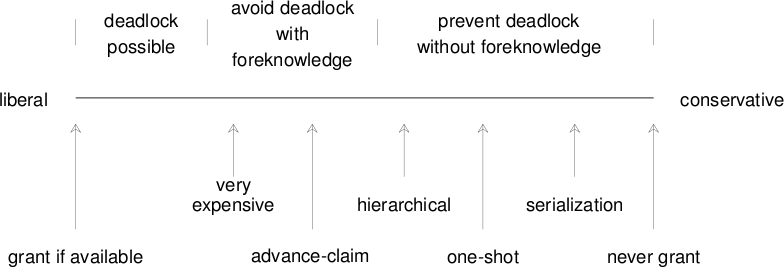
\includegraphics[width=0.6\textwidth]{./img/dot/deadlocks_conserv_lib.png}
\caption{\label{PROC_deadlocks_conserv_lib}Espectro liberal—conservador de esquemas para evitar bloqueos}
\end{figure}

Las líneas principales que describen a las estrategias para enfrentar
situaciones de bloqueo (La Red, p. 188) son:

\begin{description}
\item[Prevención] se centra en modelar el comportamiento del sistema
		para que \emph{elimine toda posibilidad} de que se produzca
		un bloqueo. Resulta en una utilización subóptima de
		recursos.
\item[Evasión] busca imponer condiciones menos estrictas que en la
	     prevención, para intentar lograr una mejor utilización de
	     los recursos. Si bien no puede evitar \emph{todas las 	     posibilidades} de un bloqueo, cuando éste se produce
	     busca \emph{evitar} sus consecuencias.
\item[Detección y recuperación] el sistema \emph{permite} que ocurran los
     bloqueos, pero busca \emph{determinar si ha ocurrido} y tomar medidas
     para eliminarlo.

     Busca despejar los bloqueos presentados para que el sistema
     continúe operando sin ellos.
\end{description}
\subsection{Prevención de bloqueos}
\label{sec-3-4-1}


Se presentan a continuación algunos algoritmos que implementan la
prevención de bloqueos.
\subsubsection{Serialización}
\label{sec-3-4-1-1}


Una manera de evitar bloqueos \emph{por completo} sería el que un sistema
operativo jamás asignara recursos a más de un proceso a la vez — Los
procesos podrían seguir efectuando cálculos o empleando recursos \emph{no rivales} (que no requieran acceso exclusivo — por ejemplo, empleo de
archivos en el disco, sin que exista un acceso directo del proceso al
disco), pero sólo uno podría obtener recursos de forma exclusiva al
mismo tiempo. Este mecanismo sería la \emph{serialización}, y la situación
antes descrita se resolvería de la siguiente manera:

\begin{enumerate}
\item \emph{A} solicita una unidad de cinta y se bloquea
\item \emph{B} solicita una unidad de cinta y se bloquea
\item El sistema operativo otorga la unidad \emph{1} a \emph{A} y lo vuelve a poner
   en ejecución
\item \emph{A} continúa procesando; termina su periodo de ejecución
\item El sistema operativo mantiene bloqueado a \emph{B}, dado que \emph{A} tiene
   un recurso
\item \emph{A} solicita otra unidad de cinta y se bloquea
\item El sistema operativo otorga la unidad \emph{2} a \emph{A} y lo vuelve a poner
   en ejecución
\item \emph{A} libera la unidad de cinta \emph{1}
\item \emph{A} libera la unidad de cinta \emph{2} (y con ello, el bloqueo de uso de
   recursos)
\item El sistema operativo otorga la unidad \emph{1} a \emph{B} y lo vuelve a
    poner en ejecución
\item \emph{B} solicita otra unidad de cinta y se bloquea
\item El sistema operativo otorga la unidad \emph{2} a \emph{B} y lo vuelve a
    poner en ejecución
\item \emph{B} libera la unidad de cinta \emph{1}
\item \emph{B} libera la unidad de cinta \emph{2}
\end{enumerate}

Si bien la serialización resuelve la situación aquí mencionada, el
mecanismo empleado es subóptimo dado que puede haber hasta \emph{n-1}
procesos esperando a que uno libere los recursos.

Un sistema que implementa una política de asignación de recursos
basada en la serialización, si bien no caerá en bloqueos mutuos, sí
tiene un peligro fuerte de caer en \emph{inanición}.
\subsubsection{Retención y espera (\emph{advance claim})}
\label{sec-3-4-1-2}


Otro ejemplo de política preventiva \emph{menos conservadora} sería la
\emph{retención y espera} o \emph{reserva} (\emph{advance claim}): que todos los
programas declaren al iniciar su ejecución qué recursos van a
requerir. Los recursos son apartados para su uso exclusivo hasta que
el proceso termina, pero el sistema operativo puede seguir atendiendo
solicitudes \emph{que no rivalicen}: si a los procesos \emph{A} y \emph{B} anteriores
se suman procesos \emph{C} y \emph{D}, pero requieren otro tipo de recursos,
podrían ejecutarse en paralelo \emph{A}, \emph{C} y \emph{D}, y una vez que \emph{A}
termine, podrían continuar ejecutando \emph{B}, \emph{C} y \emph{D}.

El bloqueo resulta ahora imposible por diseño, pero el usuario que
inició \emph{B} tiene una percepción de injusticia dado el tiempo que tuvo
que esperar para que su solicitud fuera atendida — de hecho, si \emph{A} es
un proceso de larga duración (incluso si requiere la unidad de cinta
sólo por un breve periodo), esto lleva a que \emph{B} sufra una \emph{inanición}
innecesariamente prolongada.

Además, la implementación de este mecanismo preventivo requiere que el
programador sepa por anticipado qué recursos requerirá — y esto en la
realidad muchas veces es imposible. Si bien podría diseñarse una
estrategia de lanzar procesos \emph{representantes} (o \emph{proxy}) solicitando
recursos específicos cuando éstos hicieran falta, esto sólo
transferiría la situación de bloqueo por recursos a bloqueo por
procesos — y un programador poco cuidadoso podría de todos modos
desencadenar la misma situación.
\subsubsection{Solicitud \emph{de una vez} (\emph{one-shot})}
\label{sec-3-4-1-3}
\label{PROC_one-shot}


Otro mecanismo de prevención de bloqueos sería que los recursos se
otorguen exclusivamente a aquellos procesos que \emph{no poseen ningún recurso}. Esta estrategia rompería la condición de Coffman \emph{espera por}, haciendo imposible que se presente un bloqueo.

En su planteamiento inicial, este mecanismo requería que un proceso
declarara \emph{una sola vez} qué recursos requeriría, pero posteriormente
la estrategia se modificó, permitiendo que un proceso solicite
recursos nuevamente, pero únicamente a condición de que previo a
hacerlo \emph{renuncien a los recursos} que tenían en ese momento —
Claro, pueden volver a incluirlos en la operación de solicitud.

Al haber una \emph{renuncia explícita}, se imposibilita de forma tajante
que un conjunto de procesos entre en condición de bloqueo mutuo.

Las principales desventajas de este mecanismo son:

\begin{itemize}
\item Requiere cambiar la lógica de programación para tener puntos más
  definidos de adquisición y liberación de recursos.
\item Muchas veces no basta con la \emph{readquisición} de un recurso, sino
  que es necesario \emph{mantenerlo bloqueado}. Volviendo al ejemplo de
  las unidades de cinta, un proceso que requiera ir generando un
  archivo largo no puede arriesgarse a \emph{soltarla}, pues podría ser
  entregada a otro proceso y corromperse el resultado.
\end{itemize}
\subsubsection{Asignación jerárquica}
\label{sec-3-4-1-4}


Otro mecanismo de evasión es la asignación \emph{jerárquica} de
recursos. Bajo este mecanismo, se asigna una prioridad o \emph{nivel jerárquico} a cada recurso o clase de recursos.\footnote{Incluso varios
recursos distintos, o varias clases, pueden compartir prioridad,
aunque esto dificultaría la programación. Podría verse a la \emph\{solicitud
de una vez\} como un caso extremo de asignación jerárquica, con una
jerarquía plana. } La condición básica es que, una vez que un proceso
obtiene un recurso de determinado nivel, sólo puede solicitar recursos
adicionales de niveles superiores. En caso de requerir dos
dispositivos ubicados al mismo nivel, tiene que hacerse de forma
atómica.

De este modo, si las unidades de cinta tienen asignada la prioridad
$x$, $P_1$ sólo puede solicitar dos unidades de cinta por medio de
\emph{una sóla operación}. En caso de también requerir dos unidades de
cinta el proceso $P_2$ \emph{al mismo tiempo}, al ser atómicas las
solicitudes, éstas le serán otorgadas a sólo un de los dos procesos,
por lo cual no se presentará bloqueo.

Además, el crear una jerarquía de recursos permitiría ubicar los
recursos más escasos o \emph{peleados} en la cima de la jerarquía,
reduciendo las situaciones de contención en que varios procesos
compiten por dichos recursos — sólo llegarían a solicitarlos aquellos
procesos que ya tienen \emph{asegurado} el acceso a los demás recursos que
vayan a emplear.

Sin embargo, este ordenamiento es demasiado estricto para muchas
situaciones del mundo real. El tener que renunciar a ciertos recursos
para adquirir uno de menor prioridad \emph{y volver a competir por ellos},
además de resultar contraintuitivo para un programador, resulta en
esperas frustrantes. Este mecanismo llevaría a los procesos a acaparar
recursos de baja prioridad, para evitar tener que ceder y re-adquirir
recursos más altos, por lo que conduce a una alta inanición.
\subsection{Evasión de bloqueos}
\label{sec-3-4-2}


Para la evasión de bloqueos, el sistema partiría de poseer, además de
la información descrita en el caso anterior, información acerca de
\emph{cuándo} requiere un proceso utilizar cada recurso. De este modo, el
planificador puede marcar qué orden de ejecución (esto es, qué
\emph{flujos}) entre dos o más procesos son \emph{seguros} y cuáles son
\emph{inseguros}

\begin{figure}[htb]
\centering
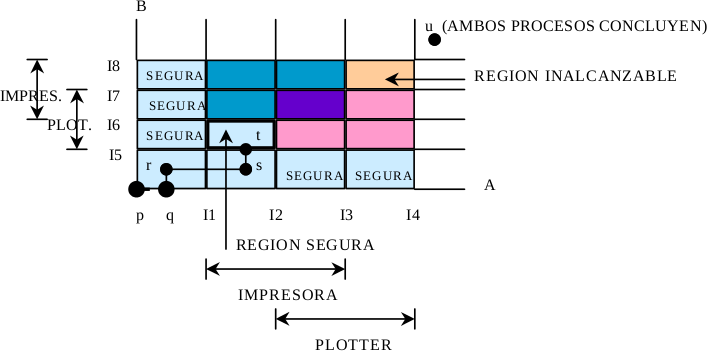
\includegraphics[width=0.7\textwidth]{./img/gnuplot/tray_proc_evasion_bloqueo.png}
\caption{\label{PROC_tray_proc_evasion_bloqueo}Evasión de bloqueos: Los procesos $A$ (horizontal) y $B$ (vertical) requieren del acceso exclusivo a un plotter y una impresora, exponiéndose a bloqueo mutuo.}
\end{figure}

El análisis de la interacción entre dos procesos se representa como en
la figura \ref{PROC_tray_proc_evasion_bloqueo}; el avance es marcado
en sentido horizontal para el proceso $A$, o vertical para el proceso
$B$; en un sistema multiprocesador, podría haber avance mutuo, y lo
se indicaría en diagonal.

En el ejemplo presentado, el proceso $A$ solicita acceso
exclusivo al scanner durante $2 \le t_A \le 7$ y a la impresora
durante $3 \le t_A \le 7.5$, mientras que $B$ solicita acceso
exclusivo a la impresora durante $2 \le t_B \le 6$ y al scanner
durante 4 $\le$ $t_B \le 7$.

Al saber cuándo reclama y libera un recurso cada proceso, se puede
marcar cuál es el área \emph{segura} para la ejecución y cuándo se
está aproximando a un área de riesgo.

En el caso mostrado, si bien el bloqueo mutuo sólo se produciría
formalmente en cualquier punto\footnote{En realidad, sólo sería
posible \emph{tocar} el márgen izquierdo o inferior de este bloque: al caer
en bloqueo mutuo, avanzar hacia su área interior resultaría
imposible. } en $3 \le t_A \le 7$, y $4 \le t_B \le 6$ (indicado con el
recuadro rojo, \emph{Bloqueo mutuo}).

Pero la existencia del recuadro que indica el bloqueo mutuo podría ser
revelada con anterioridad: si el flujo entra en el área marcada como
\emph{Bloqueo inminente}, en color naranja (en $3 \le t_A \le 7$ y $2 \le
t_B \le 6$), resulta \emph{ineludible} caer en el bloqueo mutuo. 

La región de bloqueo inminente ocurre a partir de que $A$ obtuvo el
scanner y $B$ obtuvo la impresora. Si en $t_A=2.5$ y $t_B=3$ se cede
la ejecución a $A$ por 0.5 unidades, se llegará al punto en que
solicita la impresora ($t_A=3$), y no habrá más remedio que ejecutar
$B$; al avanzar $B$ 0.5 unidades requerirá al scanner, y se habrá
desencadenado el bloqueo mutuo. Un caso análogo ocurre, claro
está, si desde el punto de inicio se ejecutara primero $B$ y luego
$A$.

Dadas las anteriores condiciones, y conociendo estos patrones de uso,
el sistema operativo evitará entrar en el área de bloqueo inminente:
el sistema mantendrá \emph{en espera} a $B$ si $t_B \le 2$ mientras $2 \le
t_A \le 6$, y mantendrá a $A$ en espera si $t_A \le 2$ cuando  $2 \le t_B
\le 6$.

La región marcada como \emph{inalcanzable} en color amarillo, no representa
ningún peligro: sólo indica aquellos estados en que resulta imposible
entrar. Incluso una vez evadido el bloqueo (por ejemplo, si $B$ fue
suspendido en $t_B = 1.8$ y $A$ avanza hasta pasar $t_A = 7$, si el
sistema operativo vuelve a dar la ejecución a $B$, este sólo podrá
avanzar hasta $t_B=2$, punto en que $B$ solicita la impresora. Para
que $B$ continúe, es necesario avanzar hasta $t_A > 7.5$ para que $B$
siga avanzando.

Este mecanismo proveería una mejor respuesta que los vistos en el
apartado de \emph{prevención de bloqueos}, pero es todavía más dificil de
aplicar en situaciones reales. Para poder implementar un sistema con
evasión de bloqueos, tendría que ser posible hacer un análisis
estático previo del código a ejecutar, y tener un listado total de
recursos estático. Estos mecanismos podrían ser efectivos en sistemas
de uso especializado, pero no en sistemas operativos (o
planificadores) genéricos.
\subsubsection{Algoritmo del banquero}
\label{sec-3-4-2-1}


Edsger Djikstra propuso un algoritmo de asignación de recursos
orientado a la evasión de bloqueos a ser empleado para el sistema
operativo THE (desarrollado entre 1965 y 1968 en la Escuela Superior
Técnica de Eindhoven, Technische Hogeschool Eindhoven), un sistema
multiprogramado organizado en anillos de privilegios. El nombre de
este algoritmo proviene de que busca que el sistema opere cuidando de
tener siempre la liquidez (nunca entrar a \emph{estados inseguros}) para
satisfacer los préstamos (recursos) solicitados por sus clientes
(quienes a su vez tienen una línea de crédito pre-autorizada por el
banco).

Este algoritmo permite que el conjunto de recursos solicitado por los
procesos en ejecución en el sistema sea mayor a los recursos
físicamente disponibles, pero a través de un monitoreo y control en su
asignación, logra este nivel de \emph{sobre-compromiso} sin poner en riesgo
la operación correcta del sistema.

Este algoritmo debe ejecutarse cada vez que un proceso solicita
recursos; el sistema evita caer en situaciones conducentes a un
bloqueo mutuo ya sea denegando o posponiendo la solicitud. El
requisito particular es que, al iniciar, cada proceso debe \emph{anunciar su reclamo máximo} (llamese \texttt{claim()}) al sistema: el número máximo
de recursos de cada tipo que va a emplear a lo largo de su ejecución —
esto sería implementado como una llamada al sistema. Una vez que un
proceso presentó su reclamo máximo de recursos, cualquier llamada
subsecuente a \texttt{claim()} falla. Claro está, si el proceso anuncia una
necesidad mayor al número existente de recursos de algún tipo, también
falla dado que el sistema no será capaz de cumplirlo.

Para el algoritmo del banquero:

\begin{description}
\item[Estado] matrices de recursos disponibles, reclamos máximos y
            asignación de recursos a los procesos en un momento dado.
\item[Estado seguro] un estado en el cual todos los procesos pueden
                   ejecutar hasta el final sin encontrar un bloqueo
                   mutuo.
\item[Estado inseguro] todo estado que no garantice que todos los
     procesos puedan ejecutar hasta el final sin encontrar un bloqueo
     mutuo.
\end{description}

Este algoritmo típicamente trabaja basado en diferentes \emph{categorías} de
recursos, y los reclamos máximos anunciados por los procesos son por
cada una de las categorías.

El estado está compuesto, por clase de recursos y por proceso, por:

\begin{description}
\item[Reclamado] número de instancias de este recurso que han sido
               reclamadas.
\item[Asignado] número de instancias de este recurso actualmente
              asignadas a procesos en ejecución.
\item[Solicitado] número de instancias de este recurso actualmente
                pendientes de asignar (solicitudes hechas y no
                cumplidas).
\end{description}

Además de esto, el sistema mantiene globalmente, por clase de
recursos:

\begin{description}
\item[Disponibles] número total de instancias de este recurso
                 disponibles al sistema.
\item[Libres] número de instancias de este recurso que no están
            actualmente asignadas a ningún proceso.
\end{description}

Cada vez que un proceso solicita recursos, se calcula cuál sería el
estado resultante de \emph{otorgar} dicha solicitud, y se otorga siempre
que:

\begin{itemize}
\item No haya reclamo por más recursos que los disponibles.
\item Ningún proceso solicite (o tenga asignados) recursos por encima de
  su reclamo.
\item La suma de los recursos \emph{asignados} por cada categoría no sea mayor
  a la cantidad de recursos \emph{disponibles} en el sistema para dicha
  categoría.
\end{itemize}

Formalmente, y volviendo a la definición de un estado seguro: un
estado \emph{es seguro} cuando hay una secuencia de procesos (denominada
\emph{secuencia segura}) tal que:

\begin{enumerate}
\item Un proceso \emph{j} puede necesariamente terminar su ejecución, incluso
   si solicitara todos los recursos que permite su reclamo, dado que
   hay suficientes recursos libres para satisfacerlo.
\item Un segundo proceso \emph{k} de la secuencia puede terminar si \emph{j}
   termina y libera todos los recursos que tiene, porque sumado a los
   recursos disponibles ahora, con aquellos que liberaría \emph{j}, hay
   suficientes recursos libres para satisfacerlo.
\item El \emph{i}-ésimo proceso puede terminar si todos los procesos
   anteriores terminan y liberan sus recursos.
\end{enumerate}

En el peor de los casos, esta secuencia segura llevaría a bloquear
todas las solicitudes excepto las del único proceso que puede avanzar
sin peligro en el orden presentado.

Se presnta un ejemplo simplificando, asumiendo sólo una clase de
procesos, e iniciando con 2 instancias libres:


\begin{center}
\begin{tabular}{lrr}
 Proceso   &  Asignado  &  Reclamando  \\
\hline
 \emph{A}  &         4  &           6  \\
 \emph{B}  &         4  &          11  \\
 \emph{C}  &         2  &           7  \\
\end{tabular}
\end{center}



\emph{A} puede terminar porque sólo requiere de 2 instancias adicionales
para llegar a las 6 que indica en su reclamo. Una vez que termine,
liberará sus 6 instancias. Se le asignan entonces las 5 que solicita a
\emph{C}, para llegar a 7. Al terminar éste, habrá 8 disponibles, y
asignándole 7 a \emph{B} se garantiza poder terminar. La secuencia (\emph{A},
\emph{C}, \emph{B}) es una secuencia segura.

Sin embargo, el siguiente estado es inseguro (asumiendo también dos
instancias libres):


\begin{center}
\begin{tabular}{lrr}
 Proceso   &  Asignado  &  Reclamado  \\
\hline
 \emph{A}  &         4  &          6  \\
 \emph{B}  &         4  &         11  \\
 \emph{C}  &         2  &          9  \\
\end{tabular}
\end{center}



\emph{A} puede terminar, pero no se puede asegurar que \emph{B} o \emph{C} puedan
hacerlo, porque incluso una vez terminando \emph{A}, se tendrían sólo 6
instancias no asignadas.

Es necesario apuntar que no hay \emph{garantía} de que continuar a partir
de este estado lleve a un bloqueo mutuo, dado que \emph{B} o \emph{C} pueden no
incrementar ya su utilización hasta cubrir su reclamo, esto es, puede
que lleguen a finalizar sin requerir más recursos, ya sea porque ya
los emplearon y liberaron, o porque el \emph{uso efectivo} de recursos
requeridos sencillamente resulte menor al del reclamo inicial.

El algoritmo del banquero, en el peor caso, puede tomar $O(n!)$,
aunque típicamente ejecuta en $O(n^2)$. Una implementación de este
algoritmo podría ser:


\begin{verbatim}
l = [1, 2, 3, 4, 5]; # Todos los procesos del sistema
s = []; # Secuencia segura
while ! l.empty? do
  p = l.select {|id| asignado[id] - reclamado[id] > libres}.first
  raise Exception, 'Estado inseguro' if p.nil?
  libres += asignado[p]
  l.delete(p)
  s.push(p)
end
puts "La secuencia segura encontrada es: %s" % s
\end{verbatim}

Hay refinamientos sobre este algoritmo que logran resultados
similares, reduciendo su costo de ejecución (se debe recordar que es
un procedimiento que puede ser llamado con muy alta frecuencia), como
el desarrollado por Habermann (ref: Finkel, p.136).

El algoritmo del banquero es un algoritmo conservador, dado que evita
entrar en un estado inseguro a pesar de que dicho estado no lleve con
certeza a un bloqueo mutuo. Sin embargo, su política es la más liberal
que permite asegurar que no se caerá en bloqueos mutuos, sin conocer el
\emph{orden y tiempo} en que cada uno de los procesos requeriría los
recursos.

Una desventaja fuerte de todos los mecanismos de evasión de bloqueos
es que requieren saber por anticipado los reclamos máximos de cada
proceso, lo cual puede no ser conocido en el momento de su ejecución.
\subsection{Detección y recuperación de bloqueos}
\label{sec-3-4-3}
\label{PROC_det_y_rec_bloq}


La detección de bloqueos es una forma de \emph{reaccionar} ante una
situación de bloqueo que ya se produjo y de buscar la mejor manera de
salir de ella. La detección de bloqueos podría ser una tarea
\emph{periódica}, y si bien no puede prevenir situaciones de bloqueo, puede
detectarlas una vez que ya ocurrieron y limitar su impacto.

Manteniendo una lista de recursos asignados y solicitados, el sistema
operativo puede saber cuando un conjunto de procesos están esperándose
mutuamente en una solicitud por recursos — al analizar estas tablas
como grafos dirigidos, se representará:

\begin{itemize}
\item Los procesos, con cuadrados.
\item Los recursos, con círculos.
\begin{itemize}
\item Puede representarse como un círculo grande a una \emph{clase} o
    \emph{categoría} de recursos, y como círculos pequeños dentro de éste a
    una \emph{serie de recursos idénticos} (p. ej. las diversas unidades de
    cinta)
\end{itemize}
\item Las flechas que van de un recurso a un proceso indican que el
  recurso \emph{está asignado} al proceso
\item Las flechas que van de un proceso a un recurso indican que el
  proceso \emph{solicita} el recurso
\end{itemize}

Cabe mencionar en este momento que, cuando se consideran categorías de
recursos, el tener la representación visual de un ciclo no implica
que haya ocurrido un bloqueo — este sólo se presenta cuando todos
los procesos involucrados están en espera mutua.

\begin{figure}[htb]
\centering
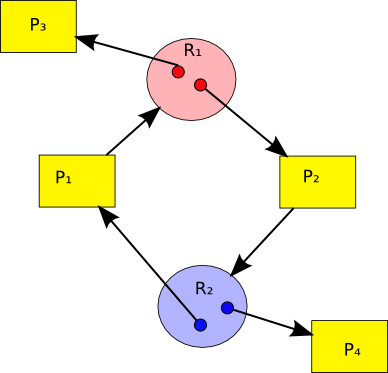
\includegraphics[width=0.5\textwidth]{./img/ciclo_no_bloqueo.png}
\caption{\label{PROC_ciclo_no_bloqueo}Al emplear categorías de recursos, un ciclo \emph{no necesariamente} indica un bloqueo}
\end{figure}

En la figura \ref{PROC_ciclo_no_bloqueo}, si bien $P_1$ y $P_2$ están
esperando que se liberen recursos de tipo $R_1$ y $R_2$, $P_3$ y $P_4$
siguen operando normalmente, y es esperable que lleguen a liberar el
recurso por el cual están esperando. En el caso ilustrado, dado que el
bloqueo se presenta únicamente al ser imposible que un proceso
\emph{libere} recursos que \emph{ya le fueron asignados}, tendría que
presentarse un caso donde todos los recursos de una misma categoría
estuvieran involucrados en una situación de espera circular, como la
ilustrada a continuación.

\begin{figure}[htb]
\centering
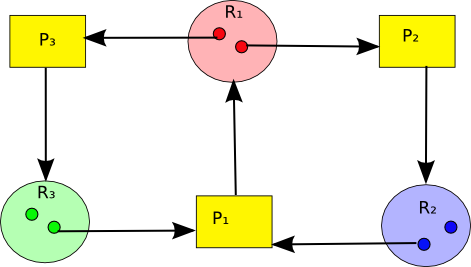
\includegraphics[width=0.5\textwidth]{./img/bloqueo_con_categorias.png}
\caption{\label{PROC_bloqueo_con_categorias}Situación en que se presenta espera circular, incluso empleando categorías de recursos}
\end{figure}

Si se tiene una representación completa de los procesos y recursos en
el sistema, la estrategia es \emph{reducir} la gráfica retirando los
elementos que no brinden información imprescindible, siguiendo la
siguiente lógica (recordar que representan una fotografía del
sistema \emph{en un momento dado}):

\begin{itemize}
\item Se retiran los procesos que no están solicitando ni tienen asignado
  ningún recurso.
\item Para todos los procesos restantes: si todos los recursos que están
  solicitando \emph{pueden ser concedidos} (esto es, no están actualmente
  asignados a otro), se reduce eliminando del grafo al proceso y a
  todas las flechas relacionadas con éste.
\item Si después de esta reducción se eliminan todos los procesos del
  grafo, entonces no hay interbloqueos y se puede continuar. En caso de
  permanecer procesos en el grafo, los procesos “irreducibles”
  constituyen la serie de procesos interbloqueados de la gráfica.
\end{itemize}

\begin{figure}[htb]
\centering
\includegraphics[width=0.7\textwidth]{./img/dot/deteccion_bloqueos.png}
\caption{\label{PROC_deteccion_bloqueos}Detección de ciclos denotando bloqueos: Grafo de procesos y recursos en un momento dado}
\end{figure}

En la gráfica \emph{Detección de ciclos denotando bloqueos}, se procede así:

\begin{itemize}
\item Se reduce por \emph{B}, dado que actualmente no está esperando a ningún
  recurso.
\item Se reduce por \emph{A} y \emph{F}, dado que los recursos por los cuales están
  esperando quedan libres en ausencia de \emph{B}.
\end{itemize}

Y queda un interbloqueo entre \emph{C}, \emph{D} y \emph{E}, en torno a los
recursos \emph{4}, \emph{5} y \emph{7}.

Nótese que \emph{reducir} un proceso del grafo no implica que éste haya
\emph{entregado} sus recursos, sino únicamente que, hasta donde se tiene
conocimiento, \emph{tiene posibilidad de hacerlo}. Los procesos que estan
esperando por recursos retenidos por un proceso pueden sufrir
inanición aún por un tiempo indeterminado.

Una vez que un bloqueo es diagnosticado, dado que los procesos no
podrán terminar por sí mismos (pues están precisamente bloqueados,
su ejecución no avanzará más), hay varias estrategias para la
recuperación:

\begin{itemize}
\item Terminar a todos los procesos bloqueados. Esta es la técnica más
  sencilla y, de cierto modo, más justa — Todos los procesos
  implicados en el bloqueo pueden ser relanzados, pero todo el estado
  del cómputo que han realizado hasta este momento se perderá.
\item \emph{Retroceder} a los procesos implicados hasta el último \emph{punto de   control} (\emph{checkpoint}) seguro conocido. Esto es posible únicamente cuando
  el sistema implementa esta funcionalidad, que tiene un elevado costo
  adicional. Cuando el estado de uno de los procesos depende de
  factores externos a éste, es imposible implementar fielmente los
  \emph{puntos de control}.

  Podría parecer que retroceder a un punto previo llevaría
  indefectiblemente a que se repita la situación — pero los bloqueos
  mutuos requieren de un orden de ejecución específico para
  aparecer. Muy probablemente, una ejecución posterior logrará
  salvar el bloqueo — y en caso contrario, puede repetirse este paso.
\item Terminar, uno por uno y no en bloque, a cada uno de los procesos
  bloqueados. Una vez que se termina uno, se evalúa la situación para
  verificar si logró romperse la situación de bloqueo, en cuyo caso la
  ejecución de los restantes continúa sin interrupción.

  Para esto, si bien podría elegirse un proceso al azar de entre los
  bloqueados, típicamente se consideran elementos adicionales como:
\begin{itemize}
\item Los procesos que demandan garantías de \emph{tiempo real} son los más
    sensibles para detener y relanzar
\item La menor cantidad de tiempo de procesador consumido hasta el
    momento. Dado que el proceso probablemente tenga que ser
    re-lanzado (re-ejecutado), puede ser conveniente \emph{apostarle} a un
    proceso que haya hecho poco cálculo (para que el tiempo que tenga
    que invertir para volver al punto actual sea mínimo).
\item Mayor tiempo restante estimado. Si se puede estimar cuánto tiempo
    de procesamiento \emph{queda pendiente}, conviene terminar al proceso
    que más le falte por hacer.
\item Menor número de recursos asignados hasta el momento. Un poco como
    criterio de justicia, y un poco partiendo de que es un proceso que
    está haciendo menor uso del sistema.
\item Prioridad más baja. Cuando hay un ordenamiento de procesos o
    usuarios por prioridades, siempre es preferible terminar un
    proceso de menor prioridad o perteneciente a un usuario poco
    importante que uno de mayor prioridad.
\item En caso de contar con la información necesaria, es siempre mejor
    interrumpir un proceso que \emph{pueda ser repetido sin pérdida de     información} que uno que la cause. Por ejemplo, es preferible
    interrumpir una compilación que la actualización de una base de
    datos.
\end{itemize}
\end{itemize}

Un punto importante a considerar es cada cuánto debe realizarse la
verificación de bloqueos. Podría hacerse:

\begin{itemize}
\item Cada vez que un proceso solicite un recurso. pero esto llevaría a un
  gasto de tiempo en este análisis demasiado frecuente.
\item Con una periodicidad fija, pero esto arriesga a que los procesos
  pasen más tiempo bloqueados.
\item Cuando el nivel del uso del CPU baje de cierto porcentaje. Esto
  indicaría que hay un nivel elevado de procesos en espera.
\item Una estrategia combinada.
\end{itemize}

Por último, si bien los dispositivos aquí mencionados requieren
bloqueo exclusivo, otra estragegia es la \emph{apropiación temporal}: tomar
un recurso asignado a determinado proceso para otorgárselo
\emph{temporalmente} a otro. Esto no siempre es posible, claro, y depende
fuertemente de la naturaleza del mismo — pero podría, por ejemplo,
interrumpirse un proceso que tiene asignada (pero inactiva) a una
impresora para otorgársela temporalmente a otro que tiene un trabajo
corto pendiente. Esto último, sin embargo, es tan sensible a detalles
de cada clase de recursos que rara vez puede hacerlo el sistema
operativo — es normalmente hecho \emph{de acuerdo} entre los procesos
competidores, por medio de algún protocolo pre-establecido.
\subsection{Algoritmo del avestruz}
\label{sec-3-4-4}


Una cuarta línea (que, por increíble que parezca, es la más común,
empleada en todos los sistemas operativos de propósito general)
es el llamado \emph{algoritmo del avestruz}: ignorar
las situaciones de bloqueo (escondiéndose de ellas como avestruz que
esconde la cabeza bajo la tierra), esperando que su ocurrencia sea
suficientemente poco frecuente, o si ocurre, que su impacto no afecte
al sistema.
\subsubsection{Justificando a los avestruces}
\label{sec-3-4-4-1}


Hay que comprender que esto ocurre porque las condiciones impuestas
por las demás estrategias resultan demasiado onerosas, el conocimiento
previo resulta insuficiente, o los bloqueos simplemente pueden
presentarse ante recursos externos y no controlados (o conocidos
siquiera) por el sistema operativo.

Ignorar la posibilidad de un bloqueo \emph{cuando su probabilidad es suficientemente baja} será preferible para los usuarios (y
programadores) ante la disyuntiva de afrontar restricciones para la
forma y conveniencia de solicitar recursos.

En este caso, se toma una decisión entre lo \emph{correcto} y lo
\emph{conveniente} — Un sistema operativo formalmente no debería permitir
la posibilidad de que hubiera bloqueos, pero la inconveniencia
presentada al usuario sería inaceptable.

Por último, cabe mencionar algo que a lo largo de todo este apartado
mencionamos únicamente de forma casual, evadiendo definiciones claras:
¿qué es un recurso? La realidad es que no está muy bien
definido. Se podría, como mencionan los ejemplos, hablar de los
clásicos recursos de acceso rival y secuencial: impresoras, cintas,
terminales seriales, etc. Sin embargo, también se pueden ver como
recursos a otras entidades administradas por el sistema operativo — el
espacio disponible de memoria, el tiempo de procesamiento, o incluso
estructuras lógicas \emph{creadas y gestionadas} por el sistema operativo,
como archivos, semáforos o monitores. Y para esos casos, prácticamente
ninguno de los mecanismos aquí analizados resolvería las
características de acceso y bloqueo necesarias.
\subsubsection{Enfrentando a los avestruces}
\label{sec-3-4-4-2}


La realidad del cómputo marca que es el programador de aplicaciones
quien debe prever las situaciones de carrera, bloqueo e inanición en
su código — El sistema operativo empleará ciertos mecanismos para
asegurar la seguridad en general entre los componentes del sistema,
pero el resto recae en las manos del programador.

Una posible salida ante la presencia del \emph{algoritmo del avestruz} es
adoptar un método \emph{defensivo} de programar. Un ejemplo de esto sería
que los programas soliciten un recurso pero, en vez de solicitarlo por
medio de una \emph{llamada bloqueante}, hacerlo por medio de una \emph{llamada no bloqueante} y, en caso de fallar ésta, esperar un tiempo aleatorio
 e intentar nuevamente acceder al recurso un número dado
de veces, y, tras \emph{n} intentos, abortar limpiamente el proceso y
notificar al usuario (evitando un bloqueo mutuo circular indefinido).

Por otro lado, hay una gran cantidad de aplicaciones de monitoreo en
espacio de usuario. Conociendo el funcionamiento esperable específico
de determinados programas es posible construir aplicaciones que los
monitoreen \emph{de una forma inteligente} y tomen acciones (ya sea alertar
a los administradores o, como se lo revisa en la sección
\ref{PROC_det_y_rec_bloq} (\emph{Detección y recuperación de bloqueos}),
abortar -y posiblemente reiniciar- la ejecución de aquellos procesos
que no puedan recuperarse).
\subsubsection{De avestruces, ingenieros y matemáticos}
\label{sec-3-4-4-3}


Esta misma contraposición puede leerse, hasta cierto punto en tono de
broma, como un síntoma de la tensión que caracteriza a nuestra
profesión: la computación nació como ciencia dentro de los
departamentos de matemáticas en diversas facultades, sin embargo, al
pasar de los años ha ido integrando cada vez más a la ingeniería. Y el
campo, una de las áreas más jóvenes pero al mismo tiempo más
prolíficas del conocimiento humano, está en una constante discusión y
definición: ¿Qué somos? ¿Matemáticos, ingenieros, o\ldots{} alguna otra
cosa?

La asignación de recursos, pues, puede verse desde el punto de vista
matemático: es un problema con un planteamiento de origen, y hay
varias estrategias distintas (los mecanismos y algoritmos descritos en
esta sección). Pueden no ser perfectos, pero el problema no ha
\emph{demostrado} ser intratable. Y un bloqueo es claramente un error — una
situación de excepción, inaceptable. Los matemáticos en nuestro árbol
genealógico académico nos llaman a no ignorar este problema, a
resolverlo sin importar la complejidad computacional.

Los ingenieros, más aterrizados en el \emph{mundo real}, tienen como parte
básica de su formación, sí, el evitar defectos nocivos — pero también
contemplan el cálculo de costos, la probabilidad de impacto, los
umbrales de tolerancia\ldots{} Para un ingeniero, si un sistema típico
\emph{corre riesgo} de caer en un bloqueo mutuo con una probabilidad $p >
0$, dejando inservibles a dos procesos en un sistema, pero debe
también considerar no sólo las fallas en hardware y en los diferentes
componentes del sistema operativo, sino que en todos los demás
programas que ejecutan en espacio de usuario, y considerando que
prevenir el bloqueo conlleva un costo adicional en complejidad para el
desarrollo o en rendimiento del sistema (dado que perderá tiempo
llevando a cabo las verificaciones ante cualquier nueva solicitud de
recursos), no debe sorprender a nadie que los ingenieros se inclinen
por adoptar la estrategia del avestruz — claro está, siempre que no
haya opción \emph{razonable}.
\section{Otros recursos}
\label{sec-3-5}


\begin{itemize}
\item \emph{Tutorial de hilos de Perl}
  \otrorec{http://perldoc.perl.org/perlthrtut.html}
  John Orwant (1998); The Perl Journal
\item \emph{Python higher level threading interface}
  \otrorec{http://docs.python.org/2/library/threading.html}
  Python Software Foundation (1990-2014); Python 2.7.6 Documentation
\item \emph{Spin Locks \& Other Forms of Mutual Exclusion}
  \otrorec{http://www.cs.fsu.edu/~baker/devices/notes/spinlock.html}
  Theodore P. Baker (2010); Florida State University
\item \emph{Dining philosophers revisited}
  \otrorec{https://dl.acm.org/citation.cfm?id=101091}
  Armando R. Gingras (1990), ACM SIGCSE Bulletin
\end{itemize}
\chapter{Planificación de procesos}
\label{sec-4}
\section{Tipos de planificación}
\label{sec-4-1}
\label{PLAN}


La \emph{planificación de procesos} se refiere a cómo determina el sistema
operativo al orden en que irá cediendo el uso del procesador a los
procesos que lo vayan solicitando, y a las políticas que empleará
para que el uso que den a dicho tiempo no sea excesivo respecto al
uso esperado del sistema.

Existen tres tipos principales de planificación:

\begin{description}
\item[A largo plazo] Decide qué procesos serán los siguientes en ser
                   iniciados. Este tipo de planificación era el más
                   frecuente en los sistemas de lotes (principalmente
                   aquellos con \emph{spool}) y multiprogramados en lotes;
                   las decisiones eran tomadas principalmente
                   considerando los requisitos pre-declarados de los
                   procesos y los que el sistema tenía libres al
                   terminar algún otro proceso. La planificación a
                   largo plazo puede llevarse a cabo con periodicidad
                   de una vez cada varios segundos, minutos e
                   inclusive horas.

		   En los sistemas de uso interactivo, casi la
                   totalidad de los que se usan hoy en día, este tipo
                   de planificación no se efectúa, dado que es
                   típicamente el usuario quien indica expresamente
                   qué procesos iniciar.

		   \begin{figure}[htb]
		   \centering
		   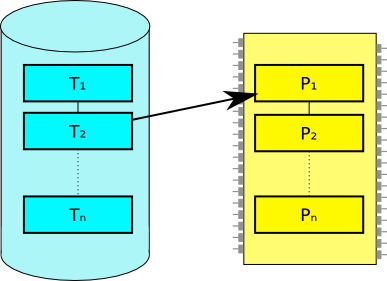
\includegraphics[width=0.6\textwidth]{./img/dot/planificador_largo_plazo.png}
		   \caption{\label{PLAN_planificador_largo_plazo}Planificador a largo plazo}
		   \end{figure}
\item[A mediano plazo] Decide cuáles procesos es conveniente \emph{bloquear}
     en determinado momento, sea por escasez/saturación de algún
     recurso (como la memoria primaria) o porque están realizando
     alguna solicitud que no puede satisfacerse momentaneamente; se
     encarga de tomar decisiones respecto a los procesos conforme
     entran y salen del estado de \emph{bloqueado} (esto es, típicamente,
     están a la espera de algún evento externo o de la finalización
     de transferencia de datos con algún dispositivo).

     En algunos textos, al \emph{planificador a mediano plazo} se le llama
     \emph{agendador} (\emph{scheduler}).

     \begin{figure}[htb]
     \centering
     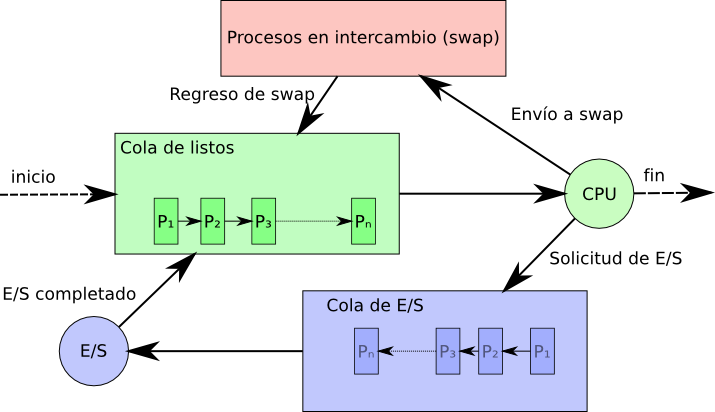
\includegraphics[width=0.7\textwidth]{./img/dot/planificador_mediano_plazo.png}
     \caption{\label{PLAN_planificador_mediano_plazo}Planificador a mediano plazo, o \emph{agendador}}
     \end{figure}
\item[A corto plazo] Decide cómo compartir \emph{momento a momento} al equipo
                   entre todos los procesos que requieren de sus
                   recursos, especialmente el procesador. La
                   planificación a corto plazo se lleva a cabo decenas
                   de veces por segundo (razón por la cual debe ser
                   código muy simple, eficiente y rápido); es el
                   encargado de planificar \emph{los procesos que están                    listos para ejecución}.

		   El \emph{planificador a corto plazo} es también
                   frecuentemente denominado \emph{despachador}
                   (\emph{dispatcher}).

		   \begin{figure}[htb]
		   \centering
		   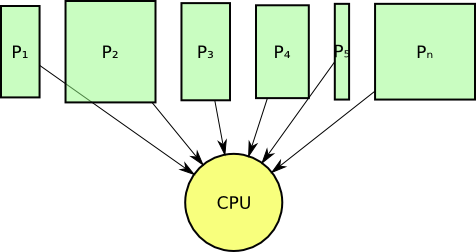
\includegraphics[width=0.5\textwidth]{./img/dot/planificador_corto_plazo.png}
		   \caption{\label{PLAN_planificador_corto_plazo}Planificador a corto plazo, o \emph{despachador}}
		   \end{figure}
\end{description}

Relacionando con los estados de un proceso abordados en la
sección \ref{PROC_estados_de_un_proceso}, y volviendo al
diagrama entonces presentado (reproducido por comodidad de referencia
en la figura \ref{PLAN_estados_proceso}), podrían ubicarse a estos tres
planificadores en las siguientes transiciones entre estados:

\begin{figure}[htb]
\centering
\includegraphics[width=0.4\textwidth]{./img/dot/estados_proceso.png}
\caption{\label{PLAN_estados_proceso}Diagrama de transición entre los estados de un proceso}
\end{figure}

\begin{enumerate}
\item El planificador a largo plazo se encarga de \emph{admitir} un nuevo
   proceso: La transición de \emph{Nuevo} a \emph{Listo}.
\item El planificador a mediano plazo maneja la \emph{activación} y \emph{bloqueo}
   de un proceso relacionado con \emph{eventos} — Esto es, las transiciones
   entre \emph{En ejecución} y \emph{Bloqueado}, y entre \emph{Bloqueado} y \emph{Listo}.
\item El planificador a corto plazo decide entre los procesos que están
   listos para ejecutarse y determina a cuál de ellos \emph{activar}, y
   detiene a aquellos que \emph{exceden su tiempo} de procesador —
   Implementa las transiciones entre los estados \emph{Listo} y \emph{En    ejecución}.
\end{enumerate}

En esta sección se trata particularmente el planificador \emph{a corto plazo}, haciendo referencia como mucho a algunos efectos del
planificador \emph{a mediano plazo}.
\subsection{Tipos de proceso}
\label{sec-4-1-1}


Como ya se ha visto, los procesos típicamente alternan entre \emph{ráfagas}
(periodos, en inglés \emph{bursts}) en que realizan principalmente cómputo
interno (están \emph{limitados por CPU}, \emph{CPU-bound}) y otras en que la
atención está puesta en transmitir los datos desde o hacia
dispositivos externos (están \emph{limitados por entrada-salida},
\emph{I/O-bound}). Dado que cuando un proceso se suspende para realizar
entrada-salida deja de estar \emph{listo} (y pasa a estar \emph{bloqueado}), y
desaparece de la atención del planificador a corto plazo, en todo
momento los procesos que están en ejecución y listos pueden separarse
en:

\begin{description}
\item[Procesos largos] Aquellos que \emph{por mucho tiempo}\footnote{¿Cuánto es
     mucho? Dependerá de las políticas generales que se definan para el
     sistema } han estado en \emph{listos} o en ejecución, esto es,
     procesos que estén en una larga ráfaga limitada por CPU.
\item[Procesos cortos] Aquellos que, ya sea que en \emph{este momento}\footnote{Y
     también, \emph{este momento} debe ser interpretado con la granularidad
     acorde al sistema } estén en una ráfaga limitada por
     entrada-salida y requieran atención meramente ocasional del
     procesador, o tienden a estar bloqueados esperando a eventos
     (como los procesos interactivos).
\end{description}

Por lo general se busca dar un tratamiento \emph{preferente} a los procesos
cortos, en particular a los interactivos. Cuando un usuario está
interactuando con un proceso, si no tiene una respuesta \emph{inmediata} a
su interacción con el equipo (sea proporcionar comandos, recibir la
respuesta a un \emph{teclazo} o mover el puntero en el GUI) su percepción
será la de una respuesta degradada.
\subsection{Midiendo la respuesta}
\label{sec-4-1-2}


Resulta intuitivo que cada patrón de uso del sistema debe seguir
políticas de planificación distintas. Por ejemplo, en el caso de un
proceso interactivo, se buscará ubicar al proceso en una \emph{cola}
preferente (para obtener un tiempo de respuesta más ágil, para mejorar
la percepción del usuario), pero en caso de sufrir demoras, es
preferible buscar dar una respuesta \emph{consistente}, aún si la respuesta
\emph{promedio} es más lenta. Esto es, si a todas las operaciones sigue una
demora de un segundo, el usuario sentirá menos falta de control si en
promedio tardan medio segundo, pero ocasionalmente hay picos de cinco.

Para este tema, en vez de emplear unidades temporales formales
(p. ej. fracciones de segundo), es común emplear \emph{ticks} y
\emph{quantums}. Esto es en buena medida porque, si bien en el campo del
cómputo las velocidades de acceso y uso efectivo cambian
constantemente, los conceptos y las definiciones permanecen. Además,
al ser ambos parámetros ajustables, una misma implementación puede
sobrevivir ajustándose a la evolución del hardware.

\begin{description}
\item[\emph{Tick}] Una fracción de tiempo durante la cual se puede realizar
            trabajo útil - Esto es, usar la CPU sin interrupción\footnote{Ignorando
            las interrupciones causadas por los dispositivos de 
            entrada y salida y otras señales que llegan a la CPU }. El tiempo
	    correspondiente a un tick está determinado por una señal (interrupción)
	    periódica, emitida por el \emph{temporizador} (timer). La frecuencia con 
	    que ocurre esta señal se establece al inicio del sistema. Por ejemplo,
	    una frecuencia de \emph{temporizador} de 100 Hertz implica que éste
	    emitirá una señal cada 10 milisegundos.
            En Linux (a partir de la versión 2.6.8), un \emph{tick} dura un
            milisegundo, en Windows, entre 10 y 15 milisegundos.
\item[\emph{Quantum}] El tiempo mínimo que se permitirá a un proceso el uso
               del procesador. En Windows, dependiendo de la clase de
               proceso que se trate, un \emph{quantum} durará entre 2 y 12
               ticks (esto es, entre 20 y 180 ms), y en Linux, entre
               10 y 200 ticks (10 y 200 milisegundos respectivamente).
\end{description}

¿Qué mecanismos o métricas se  emplean para medir el
comportamiento del sistema bajo determinado planificador? Partiendo de
los siguientes conceptos, para un proceso $p$ que requiere de un
tiempo $t$ de ejecución:

\begin{description}
\item[Tiempo de respuesta ($T$)] Cuánto tiempo total es necesario para
     completar el trabajo pendiente de un proceso $p$, incluyendo el
     tiempo que está inactivo esperando ejecución (pero está en la
     cola de procesos listos).
\item[Tiempo en espera ($E = T - t$)] También referido como \emph{tiempo      perdido}. Del tiempo de respuesta total, cuánto tiempo $p$ está
     listo y esperando ejecutar. Desde la óptica de $p$, se desearía
     que $E_p \rightarrow 0$
\item[Proporción de penalización ($P = \frac{T}{t}$)] Fracción del
     tiempo de respuesta durante la cual $p$ estuvo en espera.
\item[Proporción de respuesta ($R = \frac{t}{T}$)] Inverso de
     $P$. Fracción del tiempo de respuesta durante la cual $p$ pudo
     ejecutarse.
\end{description}

Para hacer referencia a un grupo de procesos con requisitos similares, todos
ellos requiriendo de un mismo tiempo $t$, se emplea $T(t)$,
$E(t) = T(t) - t$, $P(t) = \frac{T(t)}{t}$ y $R(t) = \frac{t}{T(t)}$.

Además de estos tiempos, expresados en relación al tiempo efectivo de
los diversos procesos del sistema, es necesario considerar también:

\begin{description}
\item[Tiempo núcleo o \emph{kernel}] Tiempo que pasa el sistema en espacio de
     núcleo, incluyendo entre otras funciones\footnote{Estas funciones
     incluyen principalmente la atención a interrupciones, el servicio
     a llamadas al sistema, y cubrir diversas tareas administrativas. }
     el empleado en decidir e implementar la política de planificación
     y los cambios de contexto.
\item[Tiempo desocupado (\emph{idle})] Tiempo en que la cola de procesos
     listos está vacía y no puede realizarse ningún trabajo.
\item[Utilización del CPU] Porcentaje del tiempo en que el CPU está
     realizando \emph{trabajo útil}. Si bien conceptualmente puede
     ubicarse dicha utilización entre 0 y 100\%, en sistemas reales se
     ha observado (Silberschatz, p.179) que se ubica en un rango
     entre el 40 y el 90\%.
\end{description}

Por ejemplo, si llegan a la cola de procesos listos:


\begin{center}
\begin{tabular}{lrr}
\hline
 Proceso  &  Ticks  &  Llegada  \\
\hline
 $A$      &      7  &        0  \\
 $B$      &      3  &        2  \\
 $C$      &     12  &        6  \\
 $D$      &      4  &       20  \\
\hline
\end{tabular}
\end{center}



Si el tiempo que toma al sistema efectuar un cambio de contexto es de
un \emph{tick}, y la duración de cada \emph{quantum} es de 5 ticks, en un
ordenamiento de ronda,\footnote{Este mecanismo se presentará en breve, en
la sección \ref{PLAN_RoundRobin}. } se observaría un resultado como el
que ilustra la figura \ref{PLAN_planificador}.

\begin{figure}[htb]
\centering
\includegraphics[width=\textwidth]{./img/ditaa/planificador.png}
\caption{\label{PLAN_planificador}Ejecución de cuatro procesos con \emph{quantums} de 5 \emph{ticks} y cambios de contexto de 2 \emph{ticks}}
\end{figure}

Al considerar al tiempo ocupado por el núcleo como un proceso más,
cuyo trabajo en este espacio de tiempo finalizó junto con los
demás,\footnote{Normalmente \emph{no} se considera al núcleo al hacer este
cálculo, dado que en este ámbito todo el trabajo que hace puede verse
como \emph{burocracia} ante los resultados deseados del sistema } se obtiene
por resultado:


\begin{center}
\begin{tabular}{lrrrrr}
 Proceso               &  $t$  &   $T$  &    $E$  &   $P$  &    $R$  \\
\hline
 $A$                   &    7  &    18  &     11  &  2.57  &  0.389  \\
 $B$                   &    3  &     7  &      4  &  2.33  &  0.429  \\
 $C$                   &   12  &    26  &     14  &  2.17  &  0.462  \\
 $D$                   &    4  &     9  &      5  &  2.25  &  0.444  \\
 Promedio \emph{útil}  &  6.5  &    15  &   8.50  &  2.31  &  0.433  \\
\hline
 Núcleo                &    6  &    32  &     26  &  5.33  &  0.188  \\
\hline
 Promedio total        &  6.4  &  18.4  &  12.00  &  2.88  &  0.348  \\
\end{tabular}
\end{center}



Abordando cada proceso, para obtener $T$ se parte del momento en que
el proceso llegó a la cola, no el punto de inicio de la línea de
tiempo. En este caso, dado que el núcleo \emph{siempre} está en ejecución,
se asume que inició también en 0.

Respecto al patrón de llegada y salida de los procesos, lo se maneja
también basado en una relación. Partiendo de una \emph{frecuencia de llegada} promedio de nuevos procesos a la cola de procesos listos
$\alpha$, y el \emph{tiempo de servicio requerido} promedio $\beta$,
se define el \emph{valor de saturación} $\rho$ como $\rho =
\frac{\alpha}{\beta}$.

Cuando $\rho = 0$, nunca llegan nuevos procesos, por lo cual el
sistema estará eventualmente \emph{desocupado}. Cuando $\rho = 1$, los procesos son
despachados al mismo ritmo al que van llegando. Cuando $\rho > 1$, el
ritmo de llegada de procesos es mayor que la velocidad a la cual la
computadora puede darles servicio, con lo cual la cola de procesos
listos tenderá a crecer (y la calidad de servicio, la proporción de
respuesta $R$, para cada proceso se decrementará).
\section{Algoritmos de planificación}
\label{sec-4-2}
\label{PLAN_alg_planif}


El planificador a corto plazo puede ser invocado cuando un proceso se
encuentra en algunas de las cuatro siguientes circunstancias:

\begin{enumerate}
\item Pasa de estar \emph{ejecutando} a estar \emph{en espera} (por ejemplo, por
   solicitar una operación de E/S, esperar a la sincronización con
   otro proceso, etc.)
\item Pasa de estar \emph{ejecutando} a estar \emph{listo} (por ejemplo, al ocurrir
   la interrupción del temporizador, o de algún evento externo)
\item Deja de estar \emph{en espera} a estar \emph{listo} (por ejemplo, al
   finalizar la operación de E/S que solicitó)
\item Finaliza su ejecución, y pasa de \emph{ejecutando} a \emph{terminado}
\end{enumerate}

En el primer y cuarto casos, el sistema operativo siempre tomará el
control\footnote{En el primer caso, el proceso entrará en el dominio del
\emph{planificador a mediano plazo}, mientras que en el cuarto saldrá
definitivamente de la lista de ejecución. }; un sistema que opera bajo
\emph{multitarea preventiva} implementará también el segundo y tercer
casos, mientras que uno que opera bajo \emph{multitarea cooperativa} no
necesariamente reconocerá dichos estados.

Ahora, para los algoritmos a continuación, cabe recordar que se trata
únicamente del \emph{despachador}. Un proceso siempre abandonará la cola de
procesos listos al requerir de un servicio del sistema.

Para todos los ejemplos a continuación, los tiempos están
dados en \emph{ticks}; no es relevante a cuánto \emph{tiempo de reloj} estos
equivalen, sino el rendimiento relativo del sistema entero ante una
carga dada.

La presente sección está basada fuertemente en el capítulo 2 de \emph{An operating systems vade mecum} (Raphael Finkel, 1988).
\subsection{Objetivos de la planificación}
\label{sec-4-2-1}


Los algoritmos que serán presentados a continuación son respuestas
que intentan, de diferentes maneras y desde distintos supuestos base,
darse a los siguientes objetivos principales (tomando en cuenta que
algunos de estos objetivos pueden ser mutuamente contradictorios):

\begin{description}
\item[Ser justo] Debe tratarse de \emph{igual manera} a todos los procesos
               que compartan las mismas características\footnote{Un
               algoritmo de planificación puede \emph{priorizar} de
               diferente manera a los procesos según distintos
               criterios, sin por ello dejar de ser justo, siempre que
               dé la misma prioridad y respuesta a procesos
               equivalentes. }, y nunca postergar indefinidamente a uno
               de ellos.
\item[Maximizar el rendimiento] Dar servicio a la mayor parte de
     procesos por unidad de tiempo.
\item[Ser predecible] Un mismo trabajo debe tomar aproximadamente la
                    misma cantidad de tiempo en completarse
                    independientemente de la carga del sistema.
\item[Minimizar la sobrecarga] El tiempo que el algoritmo pierda en
     \emph{burocracia} debe mantenerse al mínimo, dado que éste es tiempo
     de procesamiento útil perdido
\item[Equilibrar el uso de recursos] Favorecer a los procesos que
     empleen recursos subutilizados, penalizar a los que peleen por
     un recurso sobreutilizado causando contención en el sistema
\item[Evitar la postergación indefinida] Aumentar la prioridad de los
     procesos más \emph{viejos}, para favorecer que alcancen a obtener
     algún recurso por el cual estén esperando
\item[Favorecer el \emph{uso esperado} del sistema] En un sistema con
     usuarios interactivos, maximizar la prioridad de los procesos
     que sirvan a solicitudes iniciadas por éste (aún a cambio de
     penalizar a los procesos /de sistema)
\item[Dar preferencia a los procesos que \emph{podrían causar bloqueo}] Si
     un proceso de baja prioridad está empleando un recurso del
     sistema por el cual más procesos están esperando, favorecer que
     éste termine de emplearlo más rápido
\item[Favorecer a los procesos con un \emph{comportamiento deseable}] Si un
     proceso causa muchas demoras (por ejemplo, atraviesa una ráfaga
     de entrada/salida que le requiere hacer muchas llamadas a
     sistema o interrupciones), se le puede penaliza porque degrada
     el rendimiento global del sistema
\item[Degradarse suavemente] Si bien el nivel ideal de utilización del
     procesador es al 100\%, es imposible mantenerse siempre a este
     nivel. Un algoritmo puede buscar responder con la menor
     penalización a los procesos preexistentes al momento de exceder
     este umbral.
\end{description}
\subsection{Primero llegado, primero servido (\emph{FCFS})}
\label{sec-4-2-2}


El esquema más simple de planificación es el \emph{Primero llegado, primero servido} (\emph{First come, first serve}, \emph{FCFS}). Este es un mecanismo
cooperativo, con la mínima lógica posible: Cada proceso se ejecuta en
el orden en que fue llegando, y hasta que \emph{suelta el control}. El
despachador es muy simple, básicamente una cola FIFO.

Para comparar los distintos algoritmos de planificación que serán
presentados, se presentará el resultado de cada uno de ellos sobre el
siguiente juego de procesos: (Finkel 1988, p.35)


\begin{center}
\begin{tabular}{lrrrrrrr}
 Proceso   &  Tiempo de  &  \emph{t}  &  Inicio  &  Fin  &  \emph{T}  &  \emph{E}  &  \emph{P}  \\
           &    Llegada  &            &          &       &            &            &            \\
\hline
 A         &          0  &         3  &       0  &    3  &         3  &         0  &         1  \\
 B         &          1  &         5  &       3  &    8  &         7  &         2  &       1.4  \\
 C         &          3  &         2  &       8  &   10  &         7  &         5  &       3.5  \\
 D         &          9  &         5  &      10  &   15  &         6  &         1  &       1.2  \\
 E         &         12  &         5  &      15  &   20  &         8  &         3  &       1.6  \\
\hline
 Promedio  &             &         4  &          &       &       6.2  &       2.2  &      1.74  \\
\end{tabular}
\end{center}



\begin{figure}[htb]
\centering
\includegraphics[width=\textwidth]{./img/ditaa/planif_fcfs.png}
\caption{\label{PLAN_planif_fcfs}Primero llegado, primero servido (FCFS)}
\end{figure}

Si bien un esquema FCFS reduce al mínimo la \emph{sobrecarga administrativa} (que incluye tanto al tiempo requerido por el
planificador para seleccionar al siguiente proceso como el tiempo
requerido para el cambio de contexto), el rendimiento percibido por
los últimos procesos en llegar (o por procesos cortos llegados en un
momento inconveniente) resulta inaceptable.

Este algoritmo dará servicio y salida a todos los procesos siempre que
$\rho \le 1$. En caso de que se sostenga $\rho > 1$, la demora para
iniciar la atención de un proceso crecerá cada vez más, cayendo en
una cada vez mayor inanición.

FCFS tiene características claramente inadecuadas para trabajo
interactivo, sin embargo, al no requerir de hardware de apoyo (como
un temporizador) sigue siendo ampliamente empleado.
\subsection{Ronda (\emph{Round Robin})}
\label{sec-4-2-3}
\label{PLAN_RoundRobin}


El esquema \emph{ronda} busca dar una relación de respuesta buena tanto
para procesos largos como para los cortos. La principal diferencia
entre la ronda y FCFS es que en este caso sí emplea multitarea
preventiva: Cada proceso que esté en la lista de procesos listos puede
ejecutarse por un sólo \emph{quantum} ($q$). Si un proceso no ha
terminado de ejecutar al final de su \emph{quantum}, será interrumpido y
puesto al final de la lista de procesos listos, para que espere a su
turno nuevamente. Los procesos que sean \emph{despertados} por los
planificadores a mediano o largo plazo se agregarán también al final
de esta lista.

Con la misma tabla de procesos presentada en el caso anterior
(y, por ahora, ignorando la sobrecarga administrativa provocada por
los cambios de contexto) se obtienen los siguientes resultados:


\begin{center}
\begin{tabular}{lrrrrrrr}
 Proceso   &  Tiempo de  &  \emph{t}  &  Inicio  &  Fin  &  \emph{T}  &  \emph{E}  &  \emph{P}  \\
           &    Llegada  &            &          &       &            &            &            \\
\hline
 A         &          0  &         3  &       0  &    6  &         6  &         3  &       2.0  \\
 B         &          1  &         5  &       1  &   11  &        10  &         5  &       2.0  \\
 C         &          3  &         2  &       4  &    8  &         5  &         3  &       2.5  \\
 D         &          9  &         5  &       9  &   18  &         9  &         4  &       1.8  \\
 E         &         12  &         5  &      12  &   20  &         8  &         3  &       1.6  \\
\hline
 Promedio  &             &         4  &          &       &       7.6  &       3.6  &      1.98  \\
\end{tabular}
\end{center}



\begin{figure}[htb]
\centering
\includegraphics[width=\textwidth]{./img/ditaa/planif_rr1.png}
\caption{\label{PLAN_planif_rr1}Ronda (\emph{Round Robin})}
\end{figure}

La \emph{ronda} puede ser ajustada modificando la duración de
$q$. Conforme se incrementa $q$, la ronda tiende a convertirse en
FCFS — Si cada \emph{quantum} es arbitrariamente grande, todo proceso
terminará su ejecución dentro de su \emph{quantum}; por otro lado,
conforme decrece $q$, se tiene una mayor frecuencia de cambios de
contexto; esto llevaría a una mayor ilusión de tener un procesador
dedicado por parte de cada uno de los procesos, dado que cada proceso
sería incapaz de notar las \emph{ráfagas} de atención que éste le da
(avance rápido durante un periodo corto seguido de un periodo sin
avance). Claro está, el procesador simulado sería cada vez más lento,
dada la fuerte penalización que iría agregando la sobrecarga
administrativa.

Finkel (1988, p.35) se refiere a esto como el \emph{principio de la histéresis}: \emph{Hay que resistirse al cambio}. Como ya lo se mencionó,
FCFS mantiene al mínimo posible la sobrecarga administrativa, y
–aunque sea marginalmente– resulta en mejor rendimiento global.

Si se repite el análisis anterior bajo este mismo mecanismo, pero con
un \emph{quantum} de 4 \emph{ticks}, el resultado es:


\begin{center}
\begin{tabular}{lrrrrrrr}
 Proceso   &  Tiempo de  &  \emph{t}  &  Inicio  &  Fin  &  \emph{T}  &  \emph{E}  &  \emph{P}  \\
           &    Llegada  &            &          &       &            &            &            \\
\hline
 A         &          0  &         3  &       0  &    3  &         3  &         0  &       1.0  \\
 B         &          1  &         5  &       3  &   10  &         9  &         4  &       1.8  \\
 C         &          3  &         2  &       7  &    9  &         6  &         4  &       3.0  \\
 D         &          9  &         5  &      10  &   19  &        10  &         5  &       2.0  \\
 E         &         12  &         5  &      14  &   20  &         8  &         3  &       1.6  \\
\hline
 Promedio  &             &         4  &          &       &       7.2  &       3.2  &      1.88  \\
\end{tabular}
\end{center}



\begin{figure}[htb]
\centering
\includegraphics[width=\textwidth]{./img/ditaa/planif_rr4.png}
\caption{\label{PLAN_planif_rr4}Ronda (\emph{Round Robin}), con $q=4$}
\end{figure}

Si bien aumentar el \emph{quantum} mejora los tiempos promedio de
respuesta, aumentarlo hasta convertirlo en un FCFS efectivo degenera
en una penalización a los procesos cortos, y puede llevar a la
inanición cuando $\rho > 1$. Silberschatz apunta (p.188) a que
típicamente el \emph{quantum} debe mantenerse inferior a la duración
promedio del 80\% de los procesos.
\subsection{El proceso más corto a continuación (SPN)}
\label{sec-4-2-4}
\label{PLAN_spn}

(Del inglés, \emph{Shortest Process Next})

Cuando no se tiene la posibilidad de implementar multitarea
preventiva, pero se requiere de un algoritmo más \emph{justo}, contando
con información \emph{por anticipado} acerca del tiempo que requieren los
procesos que forman la lista, puede elegirse el más corto de los
presentes.

Ahora bien, es muy difícil contar con esta información antes de
ejecutar el proceso. Es más frecuente buscar \emph{caracterizar} las
necesidades del proceso: Ver si durante su historia de ejecución\footnote{Cabe recordar que todos estos mecanismos se aplican al
\emph{planificador a corto plazo}. Cuando un proceso se bloquea esperando
una operación de E/S, sigue en ejecución, y la información de
contabilidad del mismo sigue alimentándose. SPN se ``nutre''
precisamente de dicha información de contabilidad. } ha sido un proceso
tendiente a manejar ráfagas \emph{limitadas por entrada-salida} o
\emph{limitadas por procesador}, y cuál es su tendencia actual.

Para estimar el tiempo que requerirá un proceso $p$ en su próxima
invocación, es común emplear el \emph{promedio exponencial}
$e_p$. Se define un \emph{factor atenuante} $0 \le f \le 1$, que
determinará qué tan reactivo será el promedio obtenido a la última
duración; es común que este valor sea cercano a 0.9.

Si el $p$ empleó $q$ \emph{quantums} durante su última invocación,

\begin{center}
$e_p' = fe_p + (1-f)q$
\end{center}

Se puede tomar como \emph{semilla} para el $e_p$ inicial un número elegido
arbitrariamente, o uno que ilustre el comportamiento actual del
sistema (como el promedio del $e_p$ de los procesos actualmente en
ejecución). La figura \ref{PLAN_promedio_exponencial} presenta la
predicción de tiempo requerido que determinado proceso va obteniendo
en sus diversas entradas a la cola de ejecución, basado en su
comportamiento previo, con distintos factores atenuantes.

Empleando el mismo juego de datos de procesos que se ha venido
manejando como resultados de las estimaciones, se obtiene el
siguiente resultado:


\begin{center}
\begin{tabular}{lrrrrrrr}
 Proceso   &  Tiempo de  &  \emph{t}  &  Inicio  &  Fin  &  \emph{T}  &  \emph{E}  &  \emph{P}  \\
           &    Llegada  &            &          &       &            &            &            \\
\hline
 A         &          0  &         3  &       0  &    3  &         3  &         0  &       1.0  \\
 B         &          1  &         5  &       5  &   10  &         9  &         4  &       1.8  \\
 C         &          3  &         2  &       3  &    5  &         2  &         0  &       1.0  \\
 D         &          9  &         5  &      10  &   15  &         6  &         1  &       1.2  \\
 E         &         12  &         5  &      15  &   20  &         8  &         3  &       1.6  \\
\hline
 Promedio  &             &         4  &          &       &       5.6  &       1.6  &      1.32  \\
\end{tabular}
\end{center}



\begin{figure}[htb]
\centering
\includegraphics[width=\textwidth]{./img/ditaa/planif_spn.png}
\caption{\label{PLAN_planif_spn}El proceso más corto a continuación (SPN)}
\end{figure}

Como era de esperarse, SPN favorece a los procesos cortos. Sin
embargo, un proceso largo puede esperar mucho tiempo antes de ser
atendido, especialmente con valores de $\rho$ cercanos o superiores a
1 — Un proceso más largo que el promedio está predispuesto a sufrir
inanición.

\begin{figure}[htb]
\centering
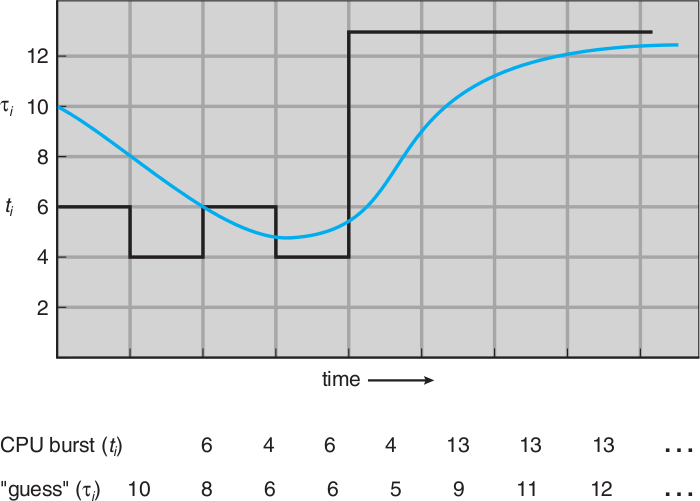
\includegraphics[width=0.6\textwidth]{./img/gnuplot/promedio_exponencial.png}
\caption{\label{PLAN_promedio_exponencial}Promedio exponencial (predicción de próxima solicitud de tiempo) de un proceso.}
\end{figure}

En un sistema poco ocupado, en que la cola de procesos listos es
corta, SPN generará resultados muy similares a los de FCFS. Sin
embargo, puede observarse en el ejemplo que con sólo una permutación
en los cinco procesos ejemplos (\emph{B} y \emph{C}), los factores de
penalización a los procesos ejemplo resultaron muy beneficiados.
\subsubsection{SPN preventivo (PSPN)}
\label{sec-4-2-4-1}


(\emph{Preemptive Shortest Process Next})

Finkel (1988, p.44) apunta a que, a pesar de que intuitivamente daría
una mayor ganancia combinar las estrategias de SPN con un esquema de
multitarea preventiva, el comportamiento obtenido es muy similar para
la amplia mayoría de los procesos. Incluso para procesos muy largos,
PSPN no los penaliza mucho más allá de lo que lo haría la ronda, y
obtiene mejores promedios de forma consistente porque, al despachar
primero a los procesos más cortos, mantiene la lista de procesos
pendientes corta, lo que lleva naturalmente a menores índices de
penalización.
\subsubsection{El más penalizado a continuación (HPRN)}
\label{sec-4-2-4-2}


(\emph{Highest Penalty Ratio Next})

En un sistema que no cuenta con multitarea preventiva, las alternativas
presentadas hasta ahora resultan invariablmente injustas: FCFS
favorece a los procesos largos, y SPN a los cortos. Un intento de
llegar a un algoritmo más balanceado es HPRN.

Todo proceso inicia su paso por la cola de procesos listos con un
valor de penalización $P = 1$. Cada vez que es obligado a esperar
un tiempo $w$ por otro proceso, $P$ se actualiza como $P =
\frac{w+t}{t}$. El proceso que se elige como activo será el que
tenga mayor $P$. Mientras $\rho < 1$, HPRN evitará que incluso los
procesos más largos sufran inanición.

En los experimentos realizados por Finkel, HPRN se sitúa siempre en
un punto medio entre FCFS y SPN; su principal desventaja se presenta
conforme crece la cola de procesos listos, ya que $P$ tiene que
calcularse para cada uno de ellos cada vez que el despachador toma una
decisión.
\subsection{Ronda egoísta (SRR)}
\label{sec-4-2-5}


(\emph{Selfish Round Robin})

Este método busca favorecer a los procesos que ya han pasado tiempo
ejecutando que a los recién llegados. De hecho, los nuevos procesos
no son programados directamente para su ejecución, sino que se les
forma en la cola de \emph{procesos nuevos}, y se avanza únicamente con la
cola de \emph{procesos aceptados}.

Para SRR se emplean los parámetros $a$ y $b$, ajustables según las
necesidades del sistema. $a$ indica el ritmo según el cual se
incrementará la prioridad de los procesos de la cola de \emph{procesos nuevos}, y $b$ el ritmo del incremento de prioridad para los \emph{procesos aceptados}. Cuando la prioridad de un proceso nuevo \emph{alcanza} a la
prioridad de un proceso aceptado, el nuevo se vuelve aceptado. Si la
cola de procesos aceptados queda vacía, se acepta el proceso nuevo con
mayor prioridad.

El comportamiento de SRR con los procesos ejemplo es:


\begin{center}
\begin{tabular}{lrrrrrrr}
 Proceso   &  Tiempo de  &  \emph{t}  &  Inicio  &  Fin  &  \emph{T}  &  \emph{E}  &  \emph{P}  \\
           &    Llegada  &            &          &       &            &            &            \\
\hline
 A         &          0  &         3  &       0  &    4  &         4  &         1  &       1.3  \\
 B         &          1  &         5  &       2  &   10  &         9  &         4  &       1.8  \\
 C         &          3  &         2  &       6  &    9  &         6  &         4  &       3.0  \\
 D         &          9  &         5  &      10  &   15  &         6  &         1  &       1.2  \\
 E         &         12  &         5  &      15  &   20  &         8  &         3  &       1.6  \\
\hline
 Promedio  &             &         4  &          &       &       6.6  &       2.6  &      1.79  \\
\end{tabular}
\end{center}



\begin{figure}[htb]
\centering
\includegraphics[width=\textwidth]{./img/ditaa/planif_srr.png}
\caption{\label{PLAN_planif_srr}Ronda egoísta (SRR) con $a = 2$ y $b = 1$}
\end{figure}

Mientras $\frac{b}{a} < 1$, la prioridad de un proceso entrante
eventualmente alcanzará a la de los procesos aceptados, y comenzará a
ejecutarse. Mientras el control va alternando entre dos o más
procesos, la prioridad de todos ellos será la misma (esto es, son
despachados efectivamente por una simple ronda).

Incluso cuando $\frac{b}{a} \ge 1$, el proceso en ejecución terminará,
y $B$ será aceptado. En este caso, este esquema se convierte en FCFS.

Si $\frac{b}{a} = 0$ (esto es, si $b = 0$), los procesos recién
llegados serán aceptados inmediatamente, con lo cual se convierte en
una ronda. Mientras $0 < \frac{b}{a} < 1$, la ronda será
\emph{relativamente egoísta}, dándole entrada a los nuevos procesos
incluso si los que llevan mucho tiempo ejecutando son muy largos (y
por tanto, su prioridad es muy alta).
\subsection{Retroalimentación multinivel (FB)}
\label{sec-4-2-6}


(\emph{Multilevel Feedback})

El mecanismo descrito en la sección anterior, la \emph{ronda egoísta},
introdujo el concepto de tener no una sino que varias colas de
procesos, que recibirán diferente tratamiento. Este mecanismo es muy
poderoso, y se emplea en prácticamente todos los planificadores en uso
hoy en día. Antes de abordar al esquema de retroalimentación
multinivel, conviene presentar cómo opera un sistema con múltiples
colas de prioridad.

\begin{figure}[htb]
\centering
\includegraphics[width=0.6\textwidth]{./img/dot/planif_multicolas.png}
\caption{\label{PLAN_planif_multicolas}Representación de un sistema con cinco colas de prioridad y siete procesos listos}
\end{figure}

La figura \ref{PLAN_planif_multicolas} ilustra cómo se presentaría
una situación bajo esta lógica: El sistema hipotético tiene cinco
colas de prioridad, y siete procesos listos para ser puestos en
ejecución. Puede haber colas vacías, como en este caso la 3. Dado que
la cola de mayor prioridad es la 0, el planificador elegirá únicamente
entre los procesos que están \emph{formados} en ella: $F$ o $C$. Sólo
cuando estos procesos terminen (o sean enviados a alguna otra cola),
el planificador continuará con aquellos que estén en las siguientes
colas.

La \emph{retroalimentación multinivel} basa su operación en más de una cola
— Pero en este caso, todas ellas tendrán el mismo tratamiento
\emph{general}, distinguiéndose sólo por su nivel de \emph{prioridad}, $C_0$ a
$C_n$. El despachador elegirá para su ejecución al proceso que esté al
frente de la cola de mayor prioridad que tenga algún proceso esperando
$C_i$, y tras un número predeterminado de ejecuciones, lo \emph{degrada} a
la cola de prioridad inmediata inferior $C_{i+1}$.

El mecanismo de retroalimentación multinivel favorece a los procesos
cortos, dado que terminarán sus tareas sin haber sido marcados como
de prioridades inferiores.

La ejecución del juego de datos con que han sido presentados los
algoritmos anteriores bajo este esquema da los siguientes resultados:



\begin{center}
\begin{tabular}{lrrrrrrr}
 Proceso   &  Tiempo de  &  \emph{t}  &  Inicio  &  Fin  &  \emph{T}  &  \emph{E}  &  \emph{P}  \\
           &    Llegada  &            &          &       &            &            &            \\
\hline
 A         &          0  &         3  &       0  &    7  &         7  &         4  &       1.7  \\
 B         &          1  &         5  &       1  &   18  &        17  &        12  &       3.4  \\
 C         &          3  &         2  &       3  &    6  &         3  &         1  &       1.5  \\
 D         &          9  &         5  &       9  &   19  &        10  &         5  &       2.0  \\
 E         &         12  &         5  &      12  &   20  &         8  &         3  &       1.6  \\
\hline
 Promedio  &             &         4  &          &       &         9  &         5  &      2.04  \\
\end{tabular}
\end{center}



Dado que ahora hay que representar la cola en la que está cada uno
de los procesos, en la figura \ref{PLAN_planif_fb_bas} se presenta
sobre cada una de las líneas de proceso la prioridad de la cola en que
se encuentra antes del \emph{quantum} a iniciar:

\begin{figure}[htb]
\centering
\includegraphics[width=\textwidth]{./img/ditaa/planif_fb_bas.png}
\caption{\label{PLAN_planif_fb_bas}Retroalimentación multinivel (FB) básica}
\end{figure}

Llama la atención que prácticamente todos los números apuntan a que
esta es una peor estrategia que las presentadas anteriormente — Los
únicos procesos beneficiados en esta ocasión son los recién llegados,
que podrán avanzar al principio, mientras los procesos más largos
serán castigados y podrán eventualmente (a mayor $\rho$) enfrentar
inanición.

Sin embargo, esta estrategia permite ajustar dos variables: Una es
la cantidad de veces que un proceso debe ser ejecutado antes de ser
\emph{degradado} a la prioridad inferior, y la otra es la duración del
\emph{quantum} asignado a las colas subsecuentes.

Otro fenómeno digno a comentar es el que se presenta a los \emph{ticks} 8,
10, 11, 13 y 14:
El despachador interrumpe la ejecución del proceso activo, para volver
a cedérsela. Esto ocurre porque, efectivamente, concluyó su \emph{quantum}
— Idealmente, el despachador se dará cuenta de esta situación de
inmediato y no iniciará un cambio de contexto \emph{al mismo proceso}. En
caso contrario, el trabajo perdido por gasto administrativo se vuelve
innecesariamente alto.

El panorama cambia al ajustar estas variables: Si se elige un
\emph{quantum} de $2^nq$, donde $n$ es el identificador de cola y $q$ la
longitud del \emph{quantum} base, un proceso largo será detenido por un
cambio de contexto al llegar a $q$, $3q$, $7q$, $15q$, etc. lo que
llevará al número total de cambios de contexto a
$\log(\frac{t(p)}{q})$, lo cual resulta atractivo frente a los
$\frac{t(p)}{q}$ cambios de contexto que tendría bajo un esquema de
ronda.

Tras de estos ajustes ante el juego de procesos con una
retroalimentación multinivel con un incremento exponencial al
\emph{quantum} se obtiene como resultado:


\begin{center}
\begin{tabular}{lrrrrrrr}
 Proceso   &  Tiempo de  &  \emph{t}  &  Inicio  &  Fin  &  \emph{T}  &  \emph{E}  &  \emph{P}  \\
           &    Llegada  &            &          &       &            &            &            \\
\hline
 A         &          0  &         3  &       0  &    4  &         4  &         1  &       1.3  \\
 B         &          1  &         5  &       1  &   10  &         9  &         4  &       1.8  \\
 C         &          3  &         2  &       4  &    8  &         5  &         3  &       2.5  \\
 D         &          9  &         5  &      10  &   18  &         9  &         4  &       1.8  \\
 E         &         12  &         5  &      13  &   20  &         8  &         3  &       1.6  \\
\hline
 Promedio  &             &         4  &          &       &         7  &         3  &       1.8  \\
\end{tabular}
\end{center}



\begin{figure}[htb]
\centering
\includegraphics[width=\textwidth]{./img/ditaa/planif_fb_exp.png}
\caption{\label{PLAN_planif_fb_exp}Retroalimentación multinivel (FB) con $q$ exponencial}
\end{figure}

Los promedios de tiempos de terminación, respuesta, espera y
penalización para este conjunto de procesos resultan mejores incluso
que los de la ronda.

En este caso, a pesar de que esta estrategia favorece a los
procesos recién llegados, al \emph{tick} 3, 9 y 10, llegan nuevos procesos,
pero a pesar de estar en la cola de mayor prioridad, no son puestos en
ejecución, dado que llegaron a la mitad del \emph{quantum} (largo) de otro
proceso.

Típicamente se emplean incrementos mucho más suaves, y de crecimiento
más controlado, como $nq$ o inlcuso $q\log(n)$, dado que en caso
contrario un proceso muy largo podría causar muy largas inaniciones
para el resto del sistema.

Para evitar la inanición, puede considerarse también la
retroalimentación en sentido inverso: Si un proceso largo fue
\emph{degradado} a la cola $C_P$ y pasa determinado tiempo sin recibir
servicio, puede \emph{promoverse} de nuevo a la cola \$C$_{\mathrm{P-1\$}}$ para que no
sufra inanición.

Hoy en día, muchos de los principales sistemas operativos operan bajo
diferentes versiones de retroalimentación multinivel, y típicamente
con hasta decenas de colas.
\subsection{Lotería}
\label{sec-4-2-7}


Los mecanismos hasta aquí descritos vienen con largas décadas de
desarrollo. Uno de los últimos algoritmos que ha sido ampliamente
difundido en unirse a esta lista es el de \emph{planificación por lotería},
publicado por \href{http://www.waldspurger.org/carl/papers/lottery-osdi94.pdf}{Carl Waldspurger y William Weihl (1994)}.

Bajo el esquema de la \emph{lotería}, cada proceso tiene un número
determinado de boletos, y cada boleto le representa una oportunidad de
jugar a la lotería. Cada vez que el planificador tiene que elegir el
siguiente proceso a poner en ejecución, elige un número al azar\footnote{Si bien operar un generador de números aleatorios en estricto sentido
sería demasiado caro para un proceso que se ejecuta decenas o cientos
de veces por segundo, para \emph{jugar} a la lotería es suficiente emplear
un generador débil pseudoaleatorio. El artículo en que este mecanismo
fue presentado presenta la implementación del algoritmo Park-Miller,
$S' = (A \times S) mod (2^{31} - 1)$ con $A = 16807$, implementado en
12 instrucciones de procesador RISC. }, y otorga el siguiente quantum
al proceso que tenga el boleto ganador. El boleto ganador \emph{no es retirado}, esto es, la probabilidad de que determinado proceso sea
puesto en ejecución no varía entre invocaciones sucesivas del
planificador.

Las prioridades pueden representarse en este esquema de forma muy
sencilla: Un proceso al que se le quiere dar mayor prioridad
simplemente tendrá más boletos; si el proceso $A$ tiene 20 boletos y
el proceso $B$ tiene 60, será tres veces más probable que el siguiente
turno toque a $B$ que a $A$.

El esquema de planificación por lotería contempla que los procesos
puedan cooperar entre sí: Si $B$ estuviera esperando un resultado de
$A$, podría transferirle sus boletos para aumentar la probabilidad de
que sea puesto en ejecución.

A pesar de su simplicidad, el esquema de planificación por lotería
resulta justo tanto a procesos cortos como a largos, y presenta una
degradación muy suave incluso en entornos de saturación. Claro, al
derivar de un proceso aleatorio, resulta imposible presentar una
comparación de este mecanismo abordados previamente.
\subsection{Esquemas híbridos}
\label{sec-4-2-8}


En líneas generales, los siete algoritmos presentados pueden
clasificarse sobre dos discriminadores primarios: Si están pensados
para emplearse en multitarea cooperativa o preventiva, y si emplean
información \emph{intrínseca} a los procesos evaluados o no lo hacen, esto
es, si un proceso es tratado de distinta forma dependiendo de su
historial de ejecución.

\begin{table}[htb]
\caption{Caracterización de los mecanismos de planificación a corto plazo} 
\begin{center}
\begin{tabular}{lll}
\hline
                       &  \textbf{No considera}  &  \textbf{Considera}       \\
                       &  \textbf{intrínseca}    &  \textbf{intrínseca}      \\
\hline
 \textbf{Cooperativa}  &  Primero llegado        &  Proceso más              \\
                       &  primero servido        &  corto (SPN),             \\
                       &  (FCFS)                 &  Proceso más              \\
                       &                         &  penalizado (HPRN)        \\
\hline
 \textbf{Preventiva}   &  Ronda (RR)             &  Proceso más corto        \\
                       &  Lotería                &  preventivo (PSPN),       \\
                       &                         &  Retroalimentación (FB),  \\
                       &                         &  Ronda egoísta (SRR)      \\
\hline
\end{tabular}
\end{center}
\end{table}


Ahora bien, estas características primarias pueden ser empleadas en
conjunto, empleando diferentes algoritmos a diferentes niveles, o
cambiándolos según el patrón de uso del sistema, aprovechando de mejor
manera sus bondades y logrando evitar sus deficiencias. A
continuación, algunos ejemplos de esquemas híbridos.
\subsubsection{Algoritmo por cola dentro de FB}
\label{sec-4-2-8-1}


Al introducir varias colas, se abre la posibilidad de que cada una de
ellas siga un esquema diferente para elegir cuál de sus procesos está
a la cabeza. En los ejemplos antes presentados, todas las colas
operaban siguiendo una ronda, pero podría contemplarse, por ejemplo,
que parte de las colas sean procesadas siguiendo una variación de PSPN
que \emph{empuje} a los procesos más largos a colas que les puedan dar
atención con menor número de interrupciones (incluso sin haberlos
ejecutado aún).

Podría emplearse un esquema SRR para las colas de menor prioridad,
siendo que ya tienen procesos que han esperado mucho tiempo para su
ejecución, para –sin que repercutan en el tiempo de respuesta de
los procesos cortos que van entrando a las colas superiores– terminen
lo antes posible su ejecución.
\subsubsection{Métodos dependientes del estado del sistema}
\label{sec-4-2-8-2}


Los parámetros de operación pueden variar también dependiendo del
estado actual del sistema, e incluso tomando en consideración valores
externos al despachador. Algunas ideas al respecto son:

\begin{itemize}
\item Si los procesos listos son \emph{en promedio} no muy largos, y el valor
  de saturación es bajo ($\rho < 1$), optar por los métodos que menos
  sobrecarga administrativa signifiquen, como FCFS o SPN (o, para
  evitar los peligros de la multitarea cooperativa, un RR con un
  \emph{quantum} muy largo). Si el despachador observa que la longitud de
  la cola excede un valor determinado (o \emph{muestra una tendencia} en
  ese sentido, al incrementarse $\rho$), cambiar a un mecanismo que
  garantice una mejor distribución de la atención, como un RR con
  \emph{quantum} corto o PSPN.
\item Usar un esquema simple de ronda. La duración de un \emph{quantum} puede
  ser ajustada periódicamente (a cada cambio de contexto, o como un
  cálculo periódico), para que la duración del siguiente \emph{quantum}
  dependa de la cantidad de procesos en espera en la lista,
  $Q=\frac{q}{n}$.

  Si hay pocos procesos esperando, cada uno de ellos recibirá un
  \emph{quantum} más largo, reduciendo la cantidad de cambios de
  contexto. Si hay muchos, cada uno de ellos tendrá que esperar menos
  tiempo para comenzar a liberar sus pendientes.

  Claro está, la duración de un \emph{quantum} no debe reducirse más allá
  de cierto valor mínimo, definido según la realidad del sistema en
  cuestión, dado que podría aumentar demasiado la carga burocrática.
\item Despachar los procesos siguiendo una ronda, pero asignarles una
  duración de \emph{quantum} proporcional a su prioridad externa (fijada
  por el usuario). Un proceso de mayor prioridad ejecutará \emph{quantums}
  más largos.
\item \emph{Peor servicio a continuación} (\emph{WSN}, \emph{Worst Service Next}). Es
  una generalización sobre varios de los mecanismos mencionados; su
  principal diferencia respecto a \emph{HPRN} es que no sólo se considera
  \emph{penalización} el tiempo que ha pasado esperando en la cola, sino
  que se considera el número de veces que ha sido interrumpido por el
  temporizador o su prioridad externa, y se considera (puede ser a
  favor o en contra) el tiempo que ha tenido que esperar por E/S u
  otros recursos. El proceso que ha sufrido del \emph{peor servicio} es
  seleccionado para su ejecución, y si varios empatan, se elige uno
  en ronda.

  La principal desventaja de \emph{WSN} es que, al considerar tantos
  factores, el tiempo requerido por un lado para recopilar todos estos
  datos, y por otro lado calcular el peso que darán a cada uno de los
  procesos implicados, puede impactar en el tiempo global de
  ejecución. Es posible acudir a WSN periódicamente (y no cada vez que
  el despachador es invocado) para que reordene las colas según
  criterios generales, y abanzar sobre dichas colas con algoritmos más
  simples, aunque esto reduce la velocidad de reacción ante cambios de
  comportamiento.
\item Algunas versiones históricas de Unix manejaban un esquema en que la
  prioridad especificada por el usuario\footnote{La \emph{lindura}, o
  \emph{niceness} de un proceso, llamada así por establecerse a través del
  comando \texttt{nice} al iniciar su ejecución, o \texttt{renice} una vez en
  ejecución } era matizada y re-evaluada en el transcurso de su
  ejecución.

  Periódicamente, para cada proceso se calcula una prioridad
  \emph{interna}, que depende de la prioridad \emph{externa} (especificada por
  el usuario) y el tiempo consumido recientemente por el
  proceso. Conforme el proceso recibe mayor tiempo de procesador, esta
  última cantidad decrece, y aumenta conforme el proceso espera (sea
  por decisión del despachador o por estar en alguna espera).

  Esta prioridad interna depende también del tamaño de la lista de
  procesos listos para su ejecución: Entre más procesos haya
  pendientes, más fuerte será la modificación que efectúe.

  El despachador ejecutará al proceso que tenga una mayor prioridad
  después de realizar estos pesos, decidiendo por ronda en caso de
  haber empates. Claro está, este algoritmo resulta sensiblemente más
  caro computacionalmente, aunque más justo, que aquellos sobre los
  cuales construye.
\end{itemize}
\subsection{Resumiendo}
\label{sec-4-2-9}
\label{PLAN_resumen_algoritmos}


En esta sección se presentan algunos mecanismos básicos de
planificación a corto plazo. Como se indica en la parte final, es muy
poco común encontrar a ninguno de estos mecanismos en un \emph{estado puro}
— Normalmente se encuentra combinación de ellos, con diferentes
parámetros según el nivel en el cual se está ejecutando.
\subsubsection{Rendimiento ante diferentes cargas de procesos}
\label{sec-4-2-9-1}


Los algoritmos presentados en el transcurso de esta sección fueron
presentados y comparados ante una determinada carga de procesos. No se
puede asumir, sin embargo, que su comportamiento será igual ante
diferentes distribuciones: Un patrón de trabajo donde predominen los
procesos cortos y haya unos pocos procesos largos probablemente se
verá mucho más penalizado por un esquema SRR (y mucho más favorecido
por un SPN o PSPN) que uno en el cual predominen los procesos largos.

\begin{figure}[htb]
\centering
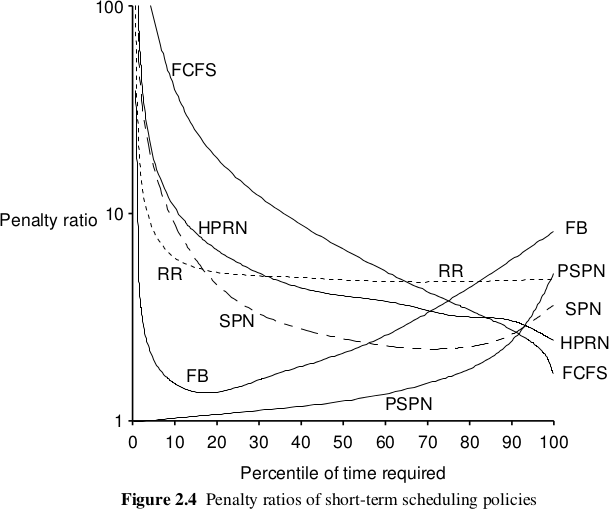
\includegraphics[width=0.7\textwidth]{./img/penalizaciones_por_algoritmo_planificador.png}
\caption{\label{PLAN_penalizaciones_por_algoritmo_planificador}Proporción de penalización registrada por cada proceso contra el porcentaje del tiempo que éste requiere (Finkel, p.33)}
\end{figure}

\begin{figure}[htb]
\centering
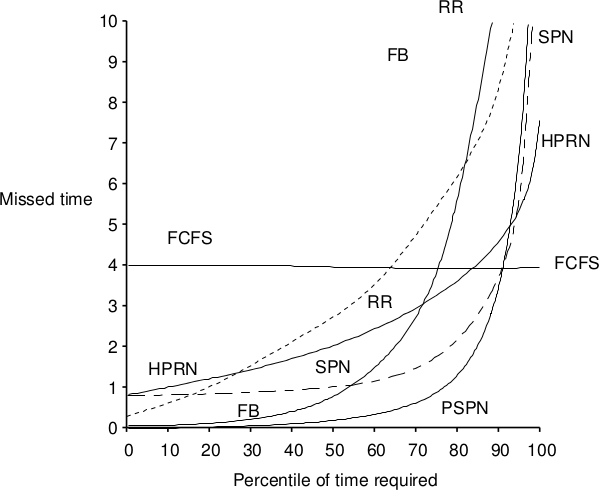
\includegraphics[width=0.7\textwidth]{./img/tiempo_en_espera_por_algoritmo_planificador.png}
\caption{\label{PLAN_tiempo_en_espera_por_algoritmo_planificador}Tiempo \emph{perdido} contra porcentaje de tiempo requerido por proceso (Finkel, p.34)}
\end{figure}

Raphael Finkel realizó estudios bajo diversas cargas de trabajo,
buscando comparar de forma \emph{significativa} estos distintos
mecanismos. Finkel simuló el comportamiento que estos algoritmos
tendrían ante 50,000 procesos generados de forma aleatoria, siguiendo
una distribución exponencial tanto en sus tiempos de llegada como
duraciones en ejecución, y manteniendo como parámetro de equilibrio un
nivel de saturación $\rho = 0.8 (\alpha = 0.8, \beta = 1.0)$,
obteniendo como resultado las figuras aquí reproducidas
(\ref{PLAN_penalizaciones_por_algoritmo_planificador} y
\ref{PLAN_tiempo_en_espera_por_algoritmo_planificador}) comparando
algunos aspectos importantes de los diferentes despachadores.
\subsubsection{Duración mínima del \emph{quantum}}
\label{sec-4-2-9-2}


La penalización por cambios de contexto en esquemas
preventivos como la \emph{ronda} puede evitarse empleando \emph{quantums}
mayores. Pero abordando la contraparte, ¿qué tan corto tiene sentido que sea un
\emph{quantum}? Con el hardware y las estructuras requeridas por los
sistemas operativos de uso general disponibles hoy en día, un cambio
de contexto requiere del orden de 10 microsegundos (Silberschatz,
p.187), por lo que incluso con el \emph{quantum} de 10ms (el más corto que
manejan tanto Linux como Windows), representa apenas la milésima parte
del tiempo efectivo de proceso.

Una estrategia empleada por Control Data Corporation para la CDC6600
(comercializada a partir de 1964, y diseñada por Seymour Cray) fue
emplear hardware especializado que permitiera efectivamente \emph{compartir el procesador}: Un sólo procesador tenía 10 \emph{juegos} de registros,
permitiéndole alternar entre 10 procesos con un \emph{quantum} efectivo
igual a la velocidad del reloj. A cada paso del reloj, el procesador
cambiaba el juego de registros. De este modo, un sólo procesador de
muy alta velocidad para su momento (1 MHz) aparecía ante las
aplicaciones como 10 procesadores efectivos, cada uno de 100 KHz,
reduciendo los costos al implementar sólamente una vez cada una de las
unidades funcionales. Puede verse una evolución de esta idea retomada
hacia mediados de la década del 2000 en los procesadores que manejan
hilos de ejecución.\footnote{Aunque la arquitecura de la CDC6600 era
\emph{plenamente superescalar}, a diferencia de los procesadores
\emph{Hyperthreading}, que será abordada brevemente en la sección
\ref{PLAN_proc_hyperthread}, en que para que dos instrucciones se
ejecuten simultáneamente deben ser de naturalezas distintas, no
requiriendo ambas de la misma \emph{unidad funcional} del CPU. El
procesador de la CDC6600 no manejaba \emph{pipelines}, sino que cada
ejecución empleaba al CPU completo }.

Esta arquitectura permitía tener multitarea real sin tener que
realizar cambios de contexto, sin embargo, al tener un \emph{nivel de concurrencia} fijo establecido en hardware no es tan fácil adecuar a
un entorno cambiante, con picos de ocupación.
\section{Planificación de hilos}
\label{sec-4-3}


Ahora bien, tras centrar toda la presente discusión en los
procesos, ¿cómo caben los \emph{hilos} en este panorama? Depende de cómo
éstos son \emph{mapeados} a procesos a ojos del planificador.

Como fue expuesto en la sección \ref{PROC_tipos_de_hilos}, hay dos
clases principales de hilo: Los \emph{hilos de usuario} o \emph{hilos verdes},
que son completamente gestionados dentro del proceso y sin ayuda del
sistema operativo, y los \emph{hilos de núcleo} o \emph{hilos de kernel}, que sí
son gestionados por el sistema operativo como si fueran
procesos. Partiendo de esto, existen tres modelos principales de
mapeo:

\begin{description}
\item[Muchos a uno] Muchos hilos son agrupados en un sólo proceso. Los
                  \emph{hilos verdes} entran en este supuesto: Para el
                  sistema operativo, hay un sólo proceso; mientras
                  tiene la ejecución, éste se encarga de repartir el
                  tiempo entre sus hilos.

		  \begin{figure}[htb]
		  \centering
		  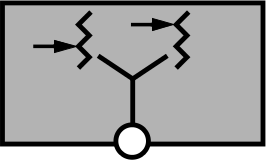
\includegraphics[width=0.3\textwidth]{./img/hilos_muchos_a_uno.png}
		  \caption{\label{PLAN_hilos_muchos_a_uno}Mapeo de hilos \emph{muchos a uno} (Imagen: Beth Plale; ver \emph{otros recursos})}
		  \end{figure}

		  Bajo este modelo, si bien el código escrito es más
                  portable entre diferentes sistemas operativos, los
                  hilos no aprovechan \emph{realmente} al paralelismo, y
                  todos los hilos pueden tener que bloquearse cuando
                  uno sólo de ellos realiza una llamada \emph{bloqueante}
                  al sistema.
\item[Uno a uno] Cada hilo es ejecutado como un \emph{proceso ligero}
               (\emph{lightweight process} o \emph{LWP}); podría dar la
               impresión de que este esquema desperdicia la principal
               característica de los hilos, que es una mayor sencillez
               y rapidez de inicialización que los procesos, sin
               embargo, la información de estado requerida para crear
               un LWP es mucho menor que la de un proceso regular, y
               mantiene como ventaja que los hilos continúan
               compartiendo su memoria, descriptores de archivos y
               demás estructuras.

	       \begin{figure}[htb]
	       \centering
	       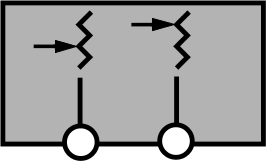
\includegraphics[width=0.3\textwidth]{./img/hilos_uno_a_uno.png}
	       \caption{\label{PLAN_hilos_uno_a_uno}Mapeo de hilos \emph{uno a uno} (Imagen: Beth Plale; ver \emph{otros recursos})}
	       \end{figure}

	       Este mecanismo permite a los hilos aprovechar las
               ventajas del paralelismo, pudiendo ejecutarse cada hilo
               en un procesador distinto, y como única condición para
               su existencia, el sistema operativo debe poder
               implementar los LWP.
\item[Muchos a muchos] Este mecanismo permite que existan hilos de ambos
     modelos: Permite la existencia de \emph{hilos unidos} (\emph{bound      threads}), en que cada hilo corresponde a un (y sólo un) LWP, y
     de \emph{hilos no unidos} (\emph{unbound threads}), de los cuales \emph{uno o      más} estarán mapeados a cada LWP.

     \begin{figure}[htb]
     \centering
     \includegraphics[width=0.3\textwidth]{./img/hilos_muchos_a_muchos.png}
     \caption{\label{PLAN_hilos_muchos_a_muchos}Mapeo de hilos \emph{muchos a muchos} (Imagen: Beth Plale; ver \emph{otros recursos})}
     \end{figure}

     El esquema \emph{muchos a muchos} proporciona las principales
     características de ambos esquemas; en caso de ejecutarse en un
     sistema que no soporte más que el modelo \emph{uno a muchos}, el
     sistema puede caer en éste como \emph{modo degradado}.
\end{description}

No se detalla en el presente texto respecto a los primeros — Cada marco de
desarrollo o máquina virtual que emplee \emph{hilos de usuario}
actuará cual sistema operativo ante ellos, probablemente con alguno
de los mecanismos ilustrados anteriormente.
\subsection{Los hilos POSIX (\texttt{pthreads})}
\label{sec-4-3-1}


La clasificiación recién presentada de modelos de mapeo entre hilos y
procesos se refleja aproximadamente en la categorización de los hilos
POSIX (\texttt{pthreads}) denominada el \emph{ámbito de contención}.

Hay dos enfoques respecto a la \emph{contención} que deben tener los
hilos, esto es: En el momento que un proceso separa su ejecución en
dos hilos, ¿debe cada uno de estos recibir la misma atención que
recibiría un proceso completo?

\begin{description}
\item[Ámbito de contención de proceso] (\emph{Process Contention Scope},
     \emph{PCS}; en POSIX, \texttt{PTHREAD\_SCOPE\_PROCESS}) Una respuesta es que
     todos los hilos deben ser atendidos sin exceder el tiempo que
     sería asignado a un sólo proceso. Un proceso que consta de varios
     hilos siguiendo el modelo \emph{muchos a uno}, o uno que \emph{multiplexa}
     varios \emph{hilos no unidos} bajo un modelo \emph{muchos a muchos}, se
     ejecuta bajo este ámbito.
\item[Ámbito de contención de sistema] (\emph{System Contention Scope},
     \emph{SCS}; en POSIX, \texttt{PTHREAD\_SCOPE\_SYSTEM}) Este ámbito es cuando,
     en contraposición, cada hilo es visto por el planificador como un
     proceso independiente; este es el ámbito en el que se ejecutarían
     los hilos bajo el modelo \emph{uno a uno}, o cada uno de los \emph{hilos      unidos} bajo un modelo \emph{muchos a muchos}, dado que los hilos son
     tratados, para propósitos de planificación, cual procesos
     normales.
\end{description}

La definición de \texttt{pthreads} apunta a que, si bien el programador
puede solicitar que sus hilos sean tratados bajo cualquiera de estos
procesos, una implementación específica puede implementar ambos o
sólo uno de los ámbitos. Un proceso que solicite que sus hilos sean
programados bajo un ámbito no implementado serán ejecutados bajo el
otro, notificando del error (pero permitiendo continuar con la
operación).

Las implementaciones de \texttt{pthreads} tanto en Windows como en Linux
sólo contemplan SCS.

Respecto a los otros aspectos mencionados en este capítulo, la
especificación \texttt{pthreads} incluye funciones por medio de las cuales
el programador puede solicitar al núcleo la prioridad de cada uno de
los hilos por separado (\texttt{pthread\_setschedprio}) e incluso solicitar
el empleo de determinado algoritmo de planificación
(\texttt{sched\_setscheduler}).
\section{Planificación de multiprocesadores}
\label{sec-4-4}


Hasta este punto, el enfoque de este capítulo se ha concentrado en la
planificación asumiendo un sólo procesador. Del mismo modo que lo que
se ha visto hasta este momento, no hay una sóla estrategia que pueda
ser vista como superior a las demás en todos los casos.

Para trabajar en multiprocesadores, puede mantenerse una sóla lista de
procesos e ir despachándolos a cada uno de los procesadores como
unidades de ejecución equivalentes e idénticas, o pueden mantenerse
listas separadas de procesos. A continuación se presentan algunos
argumentos respecto a estos enfoques.
\subsection{Afinidad a procesador}
\label{sec-4-4-1}


En un entorno multiprocesador, después de que un proceso se ejecutó
por cierto tiempo, tendrá parte importante de sus datos copiados en el
caché del procesador en el que fue ejecutado. Si el despachador
decidiera lanzarlo en un procesador que no compartiera dicho caché,
estos datos tendrían que ser \emph{invalidados} para mantener la
coherencia, y muy probablemente (por \emph{localidad de referencia}) serían
vueltos a cargar al caché del nuevo procesador.

Los procesadores actuales normalmente tienen disponibles varios
niveles de caché; si un proceso es migrado entre dos núcleos del mismo
procesador, probablemente sólo haga falta invalidar los datos en el
caché más interno (L1), dado que el caché en chip (L2) es compartido
entre los varios núcleos del mismo chip; si un proceso es migrado a
un CPU físicamente separado, será necesario invalidar también el
caché en chip (L2), y mantener únicamente el del controlador de
memoria (L3).

Pero dado que la situación antes descrita varía de computadora a
computadora, no se puede enunciar una regla general — Más allá de que
el sistema operativo debe conocer cómo están estructurados los
diversos procesadores que tiene a su disposición, y buscar realizar
las migraciones \emph{más baratas}, aquellas que tengan lugar entre los
procesadores más cercanos.

Resulta obvio por esto que un proceso que fue ejecutado en determinado
procesador vuelva a ser ejecutado en el mismo, esto es, el proceso
\emph{tiene afinidad} por cierto procesador. Un proceso que
\emph{preferentemente} será ejecutado en determinado procesador se dice que
\emph{tiene afinidad suave} por ese procesador, pero determinados patrones
de carga (por ejemplo, una mucho mayor cantidad de procesos afines a
cierto procesador que a otro, saturando su cola de procesos listos,
mientras que el segundo procesador tiene tiempo disponible) pueden
llevar a que el despachador decida activarlo en otro procesador.

Por otro lado, algunos sistemas operativos ofrecen la posibilidad de
declarar \emph{afinidad dura}, con lo cual se \emph{garantiza} a un proceso que
siempre será ejecutado en un procesador, o en un conjunto de
procesadores.

Un entorno NUMA, por ejemplo, funcionará mucho mejor si el sistema que
lo emplea maneja tanto un esquema de afinidad dura como algoritmos de
asignación de memoria que le aseguren que un proceso siempre se
ejecutará en el procesador que tenga mejor acceso a sus datos.
\subsection{Balanceo de cargas}
\label{sec-4-4-2}


En un sistema multiprocesador, la situación ideal es que todos los
procesadores estén despachando trabajos al 100\% de su capacidad. Sin
embargo, ante una definición tan rígida, la realidad es que siempre
habrá uno o más procesadores con menos del 100\% de carga, o uno o más
procesadores con procesos encolados y a la espera, o incluso ambas
situaciones.

La divergencia entre la carga de cada uno de los procesadores debe ser
lo más pequeña posible. Para lograr esto, se pueden emplear esquemas de
\emph{balanceo de cargas}: Algoritmos que analicen el estado de las colas
de procesos y, de ser el caso, transfieran procesos entre las colas
para homogeneizarlas. Claro está, el balanceo de cargas puede actuar
precisamente en sentido contrario de la afinidad al procesador, y
efectivamente puede reubicar a los procesos con afinidad suave.

Hay dos estrategias primarias de balanceo: Por un lado, la migración
activa o migración \emph{por empuje} (\emph{push migration}) consiste en una
tarea que ejecuta como parte del núcleo y periódicamente revisa el
estado de los procesadores, y en caso de encontrar un desbalance mayor
a cierto umbral, \emph{empuja} a uno o más procesos de la cola del
procesador más ocupado a la del procesador más libre. Linux ejecuta
este algoritmo cada 200 milisegundos.

Por otro lado, está la migración pasiva o migración \emph{por jalón} (\emph{pull migration}). Cuando algún procesador queda sin tareas pendientes,
ejecuta al proceso especial \emph{desocupado} (\emph{idle}). Ahora, el proceso
\emph{desocupado} no significa que el procesador detenga su actividad — Ese
tiempo puede utilizarse para ejecutar tareas del núcleo. Una de esas
tareas puede consistir en averiguar si hay procesos en espera en algún
otro de los procesadores, y de ser así, \emph{jalarlo} a la cola de este
procesador.

Ambos mecanismos pueden emplearse –y normalmente lo hacen– en el mismo
sistema. Los principales sistemas operativos modernos emplean casi
siempre ambos mecanismos.

Como sea, debe mantenerse en mente que todo balanceo de cargas que
se haga entre los procesadores conllevará una penalización en
términos de afinidad al CPU.
\subsection{Colas de procesos: ¿Una o varias?}
\label{sec-4-4-3}


En los puntos relativos al multiprocesamiento hasta ahora abordados se
parte del supuesto que hay una cola de procesos
listos por cada procesador. Si, en cambio, hubiera una cola global de
procesos listos de la cual el siguiente proceso a ejecutarse fuera
asignándose al siguiente procesador, fuera éste cualquiera de los
disponibles, podría ahorrarse incluso elegir entre una estrategia
de migración \emph{por empuje} o \emph{por jalón} — Mientras hubiera procesos
pendientes, éstos serían asignados al siguiente procesador que
tuviera tiempo disponible.

El enfoque de una sóla cola, sin embargo, no se usa en ningún sistema
en uso amplio. Esto es en buena medida porque un mecanismo así haría
mucho más difícil mantener la afinidad al procesador y restaría
flexibilidad al sistema completo.
\subsection{Procesadores con soporte a \emph{hilos hardware} (\emph{hyperthreading})}
\label{sec-4-4-4}
\label{PLAN_proc_hyperthread}


El término de \emph{hilos} como abstracción general de algo que corre con
mayor frecuencia y dentro de un mismo proceso puede llevar a una
confusión, dado que en esta sección se tocan dos temas
relacionados. Para esta subsección en particular, se hace referencia a
los \emph{hilos en hardware} que forman parte de ciertos procesadores,
ofreciendo al sistema una \emph{casi} concurrencia adicional.

Conforme han subido las frecuencias de reloj en el cómputo más allá de
lo que permite llevar al sistema entero como una sóla unidad, una
respuesta recurrente ha sido incrementar el paralelismo. Y esto no
sólo se hace proveyendo componentes completos adicionales, sino que
separando las \emph{unidades funcionales} de un procesador.

\begin{figure}[htb]
\centering
\includegraphics[width=\textwidth]{./img/ditaa/pipeline.png}
\caption{\label{PLAN_pipeline}Descomposición de una instrucción en sus cinco pasos clásicos para organizarse en un \emph{pipeline}}
\end{figure}

El flujo de una sóla instrucción a través de un procesador simple como
el MIPS puede ser dividido en cinco secciones principales, creando una
estructura conocida como \emph{pipeline} (tubería). Idealmente, en todo
momento habrá una instrucción diferente ejecutando en cada una de las
secciones del procesador, como lo ilustra la figura
\ref{PLAN_pipeline}. Las secciones en los procesadores MIPS clásicos
son:

\begin{itemize}
\item Recuperación de la instrucción (\emph{Instruction Fetch}, IF)
\item Decodificación de la instrucción (\emph{Instruction Decode}, ID)
\item Ejecución (\emph{Execution}, EX)
\item Acceso a datos (MEM)
\item Almacenamiento (Writeback, WB)
\end{itemize}

La complejidad de los procesadores actuales ha crecido ya por encima
de lo aquí delineado (el Pentium 4 tiene más de 20 etapas), sin
embargo se presenta esta separación como base para la explicación. Un
procesador puede iniciar el procesamiento de una instrucción cuando la
siguiente apenas avanzó la quinta parte de su recorrido — De este
modo, puede lograr un paralelismo interno, manteniendo idealmente
siempre ocupadas a sus partes funcionales.

Sin embargo, se ha observado que un hay patrones recurrentes que
intercalan operaciones que requieren servicio de diferentes
componentes del procesador, o que requieren de la inserción de
\emph{burbujas} porque una unidad es más lenta que las otras — Lo cual
lleva a que incluso empleando \emph{pipelines}, un procesador puede pasar
hasta el 50\% del tiempo esperando a que haya datos disponibles
solicitados a la memoria.

Para remediar esto, varias de las principales familias de
procesadores presentan a un mismo \emph{núcleo} de procesador como si
estuviera compuesto de dos o más \emph{hilos hardware} (conocidos en el
mercado como \emph{hyper-threads}). Esto puede llevar a una mayor
utilización del procesador, siguiendo patrones como el ilustrado en
la figura \ref{PLAN_hyperthread}

\begin{figure}[htb]
\centering
\includegraphics[width=\textwidth]{./img/ditaa/hyperthread.png}
\caption{\label{PLAN_hyperthread}Alternando ciclos de cómputo y espera por memoria, un procesador que implementa hilos hardware (\emph{hyperthreaded}) se presenta como dos procesadores}
\end{figure}

Hay que recordar que, a pesar de que se \emph{presenten} como hilos
independientes, el rendimiento de cada uno depende de la secuencia
particular de instrucciones del otro — No puede esperarse que el
incremento en el procesamiento sea de 2x; la figura presenta
varios puntos en que un hilo está en \emph{espera por procesador}, dado que
el otro está empleando las unidades funcionales que éste requiere.

La planificación de los hilos hardware sale del ámbito del presente
material, y este tema se presenta únicamente para aclarar un concepto que
probablemente confunda al alumno por su similitud; los hilos en
hardware implican cuestiones de complejidad tal como el ordenamiento
específico de las instrucciones, predicción de ramas de ejecución, e
incluso asuntos relativos a la seguridad, dado que se han presentado
\emph{goteos} que permiten a un proceso ejecutando en un hilo \emph{espiar} el
estado del procesador correspondiente a otro de los hilos. Para
abundar al respecto, el ámbito adecuado podría ser un texto orientado
a la construcción de compiladores (ordenamiento de instrucciones,
aprovechamiento del paralelismo), o uno de arquitectura de sistemas
(estudio del pipeline, aspectos del hardware).

Esta estrategia guarda gran similitud, y no puede evitar hacerse el
paralelo, con la \emph{compartición de procesador} empleada por la CDC6600,
presentada en la sección \ref{PLAN_resumen_algoritmos}.
\section{Tiempo real}
\label{sec-4-5}


Todos los esquemas de manejo de tiempo hasta este momento se han
enfocado a repartir el tiempo disponible entre todos los procesos que
requieren atención. Es necesario también abordar a los procesos que
\emph{requieren garantías de tiempo}: procesos que para poder
ejecutarse deben garantizar el haber tenido determinado tiempo de
proceso antes de un tiempo límite. Los procesos con estas
características se conocen como \emph{de tiempo real}.

Hay ejemplos de procesos que requieren este tipo de
planificación a todo nivel; los ejemplos más comunes son los
controladores de dispositivos y los recodificadores o reproductores de
medios (audio, video). La lógica general es la misma:

Para agendarse como un proceso con requisitos de tiempo real, éste
debe declarar sus requisitos de tiempo (formalmente, \emph{efectuar su reserva de recursos}) al iniciar su ejecución o en el transcurso de la
misma. Claro está, siendo que los procesos de tiempo real obtienen una
\emph{prioridad} mucho mayor a otros, normalmente se requerirá al iniciar
el proceso que éste \emph{declare} que durante parte de su ejecución
trabajará con restricciones de tiempo real.
\subsection{Tiempo real duro y suave}
\label{sec-4-5-1}


Supóngase que un dispositivo genera periódicamente determinada
cantidad de información y la va colocando en un área determinada de
memoria compartida (en un \emph{buffer}). Al inicializarse, su controlador
declarará al sistema operativo cuánto tiempo de ejecución le tomará
recoger y procesar dicha información, liberando el \emph{buffer} para el
siguiente ciclo de escritura del dispositivo, y la frecuencia con que
dicha operación tiene que ocurrir.

En un sistema capaz de operar con garantías de tiempo real, si el
sistema operativo puede \emph{garantizar} que en ese intervalo le otorgará
al proceso en cuestión suficiente tiempo para procesar esta
información, el proceso se ejecuta; en caso contrario, recibe un error
\emph{antes de que esto ocurra} por medio del cual podrá alertar al usuario.

Los sistemas en que el tiempo máximo es garantizable son conocidos
como de \emph{tiempo real duro}.

La necesidad de atención en tiempo real puede manejarse \emph{periódica}
(por ejemplo, \emph{requiero del procesador por 30ms cada segundo}), o
\emph{aperiódica}, por ocurrencia única (\emph{necesito que este proceso, que tomará 600ms, termine de ejecutarse en menos de 2s}).

Realizar una reserva de recursos requiere que el planificador sepa con
certeza cuánto tiempo toma realizar las tareas de sistema que
ocurrirán en el periodo en cuestión. Cuando entran en juego algunos
componentes de los sistemas de propósito general que tienen una
latencia con variaciones impredecibles (como el almacenamiento en
disco o la memoria virtual) se vuelve imposible mantener las garantías
de tiempo ofrecidas. Por esta razón, en un sistema operativo de
propósito general empleando hardware estándar \emph{no es posible}
implementar tiempo real duro.

Para solventar necesidades como las expresadas en sistemas de uso general, el
\emph{tiempo real suave} sigue requiriendo que los procesos críticos
reciban un trato prioritario por encima de los processos comunes;
agendar a un proceso con esta prioridad puede llevar a la inanición de
procesos de menor prioridad y un comportamiento que bajo ciertas
métricas resultaría \emph{injusto}. Un esquema de tiempo real suave puede
implementarse a través de un esquema similar al de la
\emph{retroalimentación multinivel}, con las siguientes particularidades:

\begin{itemize}
\item La cola de tiempo real recibe prioridad sobre todas las demás colas
\item La prioridad de un proceso de tiempo real \emph{no se degrada} conforme
  se ejecuta repetidamente
\item La prioridad de los demás procesos \emph{nunca llegan a subir} al nivel
  de tiempo real por un proceso automático (aunque sí puede hacerse
  por una llamada explícita)
\item La latencia de despacho debe ser mínima
\end{itemize}

Casi todos los sistemas operativos en uso amplio hoy en día ofrecen
facilidades básicas de tiempo real suave.
\subsection{Sistema operativo interrumpible (\emph{prevenible})}
\label{sec-4-5-2}


Para que la implementación de tiempo real suave sea apta para estos
requisitos es necesario modificar el comportamiento del sistema
operativo. Cuando un proceso de usuario hace una llamada al sistema, o
cuando una interrupción corta el flujo de ejecución, hace falta que el
sistema procese completa la rutina que da servicio a dicha solicitud
antes de que continúe operando. Se dice entonces que el sistema
operativo \emph{no es prevenible} o \emph{no es interrumpible}.

Para lograr que el núcleo pueda ser interrumpido para dar el control
de vuelta a procesos de usuario, un enfoque fue el poner \emph{puntos de interrupción} en los puntos de las funciones del sistema donde fuera
seguro, tras asegurarse que las estructuras estaban en un estado
estable. Esto, sin embargo, no modifica en mucho la situación porque
estos puntos son relativamente pocos, y es muy difícil reestructurar
su lógica para permitir puntos de prevención adicionales.

Otro enfoque es hacer al núcleo entero completamente interrumpible,
asegurándose de que, a lo largo de todo su código, todas las
modificaciones a estructuras internas estén protegidas por mecanismos
de sincronización, como los estudiados en la sección \ref{PROC_concurrencia}. Este
método ralentiza varios procesos del núcleo, pero es mucho más
flexible, y ha sido adoptado por los diversos sistemas
operativos. Tiene la ventaja adicional de que permite que haya \emph{hilos}
del núcleo corriendo de forma concurrente en todos los procesadores
del sistema.
\subsection{Inversión de prioridades}
\label{sec-4-5-3}


Un efecto colateral de que las estructuras del núcleo estén
protegidas por mecanismos de sincronización es que puede presentarse
la \emph{inversión de prioridades}. Esto es:

\begin{itemize}
\item Un proceso \emph{A} de baja prioridad hace una llamada al sistema, y es
  interrumpido a la mitad de dicha llamada
\item Un proceso \emph{B} de prioridad \emph{tiempo real} hace una segunda llamada
  al sistema, que requiere de la misma estructura que la que tiene
  bloqueada \emph{A}
\end{itemize}

Al presentarse esta situación, \emph{B} se quedará esperando hasta que \emph{A}
pueda ser nuevamente agendado — Esto es, un proceso de alta prioridad
no podrá avanzar hasta que uno de baja prioridad libere su recurso.

La respuesta introducida por Solaris 2 a esta situación a este
fenómeno es la \emph{herencia de prioridades}: Todos los procesos que estén
accesando (y, por tanto, bloqueando) recursos requeridos por un
proceso de mayor prioridad, serán tratados como si fueran de la
prioridad de dicho recurso \emph{hasta que terminen de utilizar el recurso en cuestión}, tras lo cual volverán a su prioridad nativa.
\section{Otros recursos}
\label{sec-4-6}


\begin{itemize}
\item \emph{Simulation of CPU Process scheduling}
  \otrorec{http://stimulationofcp.sourceforge.net/}
  P. A. Krishnan
  (1999-2009); programa en Java desarrollado para un curso de Sistemas
  Operativos, presentando la simulación de distintos algoritmos de
  planificación.
\item \emph{Thread Scheduling (ctd): quanta, switching and scheduling   algorithms}
  \otrorec{http://www.javamex.com/tutorials/threads/thread_scheduling_2.shtml}
  Neil Coffey (2013); Javamex tutorial and performance information
\item \emph{Microprocessor Design / Pipelined Processors}
  \otrorec{http://en.wikibooks.org/wiki/Microprocessor_Design/Pipelined_Processors}
  WikiBooks.org (2007-2013)
\item \emph{Thread scheduling and synchronization}
  \otrorec{http://www.cs.indiana.edu/classes/b534-plal/ClassNotes/sched-synch-details4.pdf}
  Beth Plale (2003); Indiana University
\item \emph{Páginas de manual} de Linux:
\begin{itemize}
\item Hilos POSIX (\texttt{pthreads})
    \otrorec{http://man7.org/linux/man-pages/man7/pthreads.7.html}
\item Modificación del ámbito de contención (\texttt{pthread\_attr\_setscope})
    \otrorec{http://man7.org/linux/man-pages/man3/pthread_attr_setscope.3.html}
\item Interfaz para solicitar cambios a los parámetros y políticas de
    planificación (\texttt{sched\_setscheduler})
    \otrorec{http://man7.org/linux/man-pages/man2/sched_setscheduler.2.html}
\end{itemize}
\item \emph{Windows Internals, 6th edition}
  \otrorec{http://technet.microsoft.com/en-us/sysinternals/bb963901.aspx}
  Mark Russinovich, David A. Solomon y Alex Ionescu (2012); por
  Microsoft Press. El capítulo 5 aborda a profundidad los temas de
  hilos y procesos bajo Windows, y está disponible como ejemplo del
  libro para su descarga en la página referida.
\item \emph{Optimizing preemption}
  \otrorec{https://lwn.net/Articles/563185/}
  Jonathan Corbet (2013), \emph{Linux Weekly News}
\end{itemize}
\chapter{Administración de memoria}
\label{sec-5}
\section{Funciones y operaciones del administrador de memoria}
\label{sec-5-1}
\label{MEM}

El único espacio de almacenamiento que el procesador puede utilizar
directamente, más allá de los registros (que si bien le son internos y
sumamente rápidos, son de capacidad demasiado limitada) es la memoria
física. Todas las arquitecturas de procesador tienen instrucciones
para interactuar con la memoria, pero ninguna lo tiene para hacerlo
con medios \emph{persistentes} de almacenamiento, como las unidades de
disco. Cabe mencionar que cuando se encuentre en un texto
referencia al \emph{almacenamiento primario} siempre se referirá a la
memoria, mientras que el \emph{almacenamiento secundario} se refiere a los
discos u otros medios de almacenamiento persistente.

Todos los programas a ejecutar deben cargarse a la memoria
del sistema antes de ser utilizados. En este capítulo se mostrará cómo
el sistema operativo administra la memoria para permitir que varios
procesos la compartan — Esta tarea debe preverse desde el proceso de
compilación de los programas (en particular, la fase de
\emph{ligado}). Hoy en día, además, casi todos los sistemas operativos
emplean implementaciones que requieren de hardware especializado — La
\emph{Unidad de Manejo de Memoria} (MMU). Se describirá cómo se manejaban
los sistemas multitarea antes de la universalización de las MMU, y qué
rol juegan hoy en día.

En esta primer sección se presentarán algunos conceptos base que 
se emplearán en las secciones subsecuentes.
\subsection{Espacio de direccionamiento}
\label{sec-5-1-1}


La memoria está estructurada como un arreglo direccionable de
bytes. Esto es, al solicitar el contenido de una dirección
específica de memoria, el hardware entregará un byte (8 bits), y
no menos. Si se requiere hacer una operación sobre \emph{bits} específicos,
se deberá solicitar y almacenar bytes enteros. En algunas
arquitecturas, el \emph{tamaño de palabra} es mayor — Por ejemplo, los
procesadores Alpha incurrían en \emph{fallas de alineación} si se
solicitaba una dirección de memoria no alineada a 64 bits, y toda
llamada a direcciones \emph{mal alineadas} tenía que ser \emph{atrapada} por el
sistema operativo, re-alineada, y entregada.

Un procesador que soporta un \emph{espacio de direccionamiento} de 16 bits
puede referirse \emph{directamente} a hasta $2^{16}$ bytes, esto es, a
hasta 65,536 bytes (64KB). Estos procesadores fueron comunes en las
décadas de 1970 y 1980 — Los más conocidos incluyen al Intel 8080 y
8085, Zilog Z80, MOS 6502 y 6510, y Motorola 6800. Hay que recalcar
que estos procesadores son reconocidos como procesadores de \emph{8 bits},
pero con \emph{espacio de direccionamiento} de 16 bits. El procesador
empleado en las primeras PC, el Intel 8086, manejaba un
direccionamiento de 20 bits (hasta 1024KB), pero al ser una
arquitectura \emph{real} de 16 bits requería del empleo de \emph{segmentación}
para alcanzar toda su memoria.

Con la llegada de la era de las \emph{computadoras personales}, diversos
fabricantes introdujeron a mediados de los años 1980 los procesadores
con arquitectura de 32 bits. Por ejemplo, la arquitectura IA-32 de Intel tiene su 
inicio oficial con el procesador 80386 (o simplemente 386). 
Este procesador podía referenciar desde el punto de vista teórico 
hasta $2^{32}$ bytes (4GB) de RAM. No obstante, debido a las 
limitaciones tecnológicas (y tal vez estratégicas) para producir 
memorias con esta capacidad, tomó más de veinte años para que las 
memorias ampliamente disponibles alcanzaran dicha capacidad.

Hoy en día, los procesadores dominantes son de 32 o 64 bits. En el caso de
los procesadores de 32 bits, sus registros pueden referenciar hasta
4,294,967,296 bytes (4GB) de RAM, que está ya dentro de los 
parámetros de lo esperable hoy en día. Una arquitectura de 
32 bits sin extensiones adicionales no puede emplear una memoria 
de mayor capacidad. No obstante, a través de un mecanismo llamado \emph{PAE}
(Extensión de Direcciónes Físicas, \emph{Physical Address Extension})
permite extender esto a rangos de hasta $2^{52}$ bytes a cambio de 
un nivel más de indirección.

Un procesador de 64 bits podría direccionar hasta
18,446,744,073,709,551,616 bytes (16 Exabytes). Los procesadores
comercialmente hoy en día no ofrecen esta capacidad de
direccionamiento principalmente por un criterio económico: Al resultar
tan poco probable que exista un sistema con estas capacidades, los
chips actuales están limitados a entre $2^{40}$ y $2^{48}$ bits — 1 y
256 terabytes. Esta restricción debe seguir teniendo sentido económico
por muchos años aún.
\subsection{Hardware: de la unidad de manejo de memoria (MMU)}
\label{sec-5-1-2}


Con la introducción de sistemas multitarea, es decir, dos o más 
programas ejecutandose, se vio la necesidad de tener más de un
programa cargado en memoria. Esto conlleva que el sistema operativo
junto con información del programa a ejecutar debe resolver cómo
ubicar los programas en la memoria física disponible.

Luego ha sido necesario emplear más memoria de la que está directamente disponible, 
con el propósito de ofrecer a los procesos más espacio de lo que puede 
direccionar /la arquitectura (hardware) empleada. Por otro lado, 
la abstracción de un espacio virtualmente ilimitado para realizar sus
operaciones incluso cuando la memoria \emph{real} es mucho menor a la
solicitada, y por último, la ilusión de tener un bloque contiguo e
ininterrumpido de memoria, cuando en realidad puede haber alta
\emph{fragmentación}.

Se explicará cómo la MMU cubre estas necesidades, y qué mecanismos
emplea para lograrlo — Y qué cuidados se deben conservar, incluso como
programadores de aplicaciones en lenguajes de alto nivel, para aprovechar de la
mejor manera estas funciones (y evitar, por el contrario, que los
programas se vuelvan lentos por no manejar la memoria
correctamente).

La MMU es también la encargada de verificar que un proceso no tenga
acceso a leer o modificar los datos de otro — Si el sistema operativo
tuviera que verificar cada una de las instrucciones ejecutadas por
un programa para evitar errores en el acceso a la memoria, la 
penalización en velocidad sería demasiado severa\footnote{Y de hecho está 
demostrado que no puede garantizarse que una verificación estática sea
suficientemente exhaustiva }.

Una primer aproximación a la protección de acceso se implementa usando
un \emph{registro base} y un \emph{registro límite}: Si la arquitectura ofrece dos
registros del procesador que sólo pueden ser modificados por el
sistema operativo (Esto es, el hardware define la modificación de
dichos registros como una operación privilegiada que requiere estar
ejecutando en \emph{modo supervisor}), la MMU puede comparar sin penalidad \emph{cada  acceso a memoria} para verificar que esté en el rango permitido.

Por ejemplo, si a un proceso le fue asignado un espacio de memoria de
64K (65535 bytes) a partir de la dirección 504214 (492K), el \emph{registro base} contendría 504214, y el \emph{registro límite} 65535. Si hubiera una
instrucción por parte de dicho proceso que solicitara una dirección
menor a 504214 o mayor a 569749 (556K), la MMU lanzaría una excepción
o \emph{trampa} interrumpiendo el procesamiento, e indicando al sistema
operativo que ocurrió una \emph{violación de segmento} (\emph{segmentation fault})\footnote{¿Por qué \emph{de segmento}? Ver la sección \ref{MEM_segmentacion} }. El sistema operativo entonces
procedería a terminar la ejecución del proceso, reclamando todos los
recursos que tuviera asignados y notificando a su usuario.

\begin{figure}[htb]
\centering
\includegraphics[width=\textwidth]{./img/ditaa/mem_base_a_limite.png}
\caption{\label{MEM_mem_base_a_limite}Espacio de direcciones válidas para el proceso 3 definido por un registro base y un registro límite}
\end{figure}
\subsection{La memoria \emph{caché}}
\label{sec-5-1-3}


Hay otro elemento en la actualidad se asume como un hecho: La memoria
\emph{caché}. Si bien su manejo es (casi) transparente para el sistema
operativo, es muy importante mantenerlo en mente.

Conforme el procesador avanza en la ejecución de las instrucciones
 (aumentando el valor almacenado en el registro de conteo de instrucción), se 
producen accesos a memoria. Por un lado, tiene que buscar en
memoria la siguiente instrucción a ejecutar. Por otro lado, estas
instrucciones pueden requerirle uno o más operadores adicionales que
deban ser leídos de la memoria. Por último, la instrucción puede
requerir guardar su resultado en cierta dirección de memoria.

Hace años esto no era un problema — La velocidad del procesador
estaba básicamente sincronizada con la del manejador de memoria, y el
flujo podía mantenerse básicamente estable. Pero conforme los
procesadores se fueron haciendo más rápidos, y conforme se ha
popularizado el procesamiento en paralelo, la tecnología de la memoria 
no ha progresado a la misma velocidad. La memoria de alta velocidad es
demasiado cara, e incluso las distancias de unos pocos centímetros se
convierten en obstáculos insalvables por la velocidad máxima de los
electrones viajando por pistas conductoras.

Cuando el procesador solicita el contenido de una dirección de memoria
y esta no está aún disponible, \emph{tiene que detener su ejecución}
(\emph{stall}) hasta que los datos estén disponibles. El CPU no puede, a
diferencia del sistema operativo, ``congelar'' todo y guardar el estado
para atender a otro proceso: Para el procesador, la lista de
instrucciones a ejecutar es estrictamente secuencial, y todo tiempo
que requiere esperar a una transferencia de datos es tiempo perdido.

La respuesta para reducir esa espera es la \emph{memoria caché}. Esta es
una memoria de alta velocidad, situada \emph{entre} la memoria principal y el
procesador propiamente, que guarda copias de las \emph{páginas} que van
siendo accesadas, partiendo del principio de la \emph{localidad de referencia}:

\begin{description}
\item[Localidad temporal] Es probable que un recurso que fue empleado
     recientemente vuelva a ser empleado en un futuro cercano.
\item[Localidad espacial] La probabilidad de que un recurso \emph{aún no      requerido} sea accesado es mucho mayor si fue requerido algún
     recurso cercano.
\item[Localidad secuencial] Un recurso, y muy particularmente la
     memoria, tiende a ser requerido de forma secuencial.
\end{description}

\begin{figure}[htb]
\centering
\includegraphics[width=0.7\textwidth]{./img/localidad_de_referencia.png}
\caption{\label{MEM_localidad_de_referencia}Patrones de acceso a memoria, demostrando la localidad espacial / temporal (Silberschatz, p.350)}
\end{figure}

Aplicando el concepto de localidad de referencia, cuando el procesador solicita
al hardware determinada dirección de memoria, el hardware no sólo
transfiere a la memoria caché el byte o palabra solicitado, sino que
transfiere un bloque o \emph{página} completo.

Cabe mencionar que hoy en día (particularmente desde que se detuvo la
\emph{guerra de los Megahertz}), parte importante del diferencial en precios
de los procesadores líderes en el mercado es la cantidad de memoria caché de
primero y segundo nivel con que cuentan.
\subsection{El espacio en memoria de un proceso}
\label{sec-5-1-4}
\label{MEM_espacio_en_memoria}


Cuando un sistema operativo inicia un proceso, no se limita a volcar
el archivo ejecutable a memoria, sino que tiene que proporcionar la
estructura para que éste vaya guardando la información de estado
relativa a su ejecución.

\begin{description}
\item[Sección (o segmento) de texto] Es el nombre que recibe la imagen en memoria de
     las instrucciones a ser ejecutadas. Usualmente, la sección de
     texto ocupa las direcciones \emph{más bajas} del espacio en memoria.
\item[Sección de datos] Espacio fijo preasignado para las variables
     globales y datos incializados (como las cadena de caracteres por ejemplo). 
     Este espacio es fijado en tiempo de compilación, y no
     puede cambiar (aunque los datos que cargados allí sí cambian en el tiempo
     de vida del proceso)
\item[Espacio de \emph{libres}] Espacio de memoria que se emplea
     para la asignación dinámica de memoria \emph{durante la ejecución} del
     proceso. Este espacio se ubica por encima de la sección de datos,
     y \emph{crece hacia arriba}. Este espacio es conocido en inglés como
     el \emph{Heap}.

     Cuando el programa es escrito en lenguajes que requieren \emph{manejo      dinámico manual de la memoria} (como C), esta área es la que se maneja a
     través de las llamadas de la familia de \texttt{malloc} y \texttt{free}. En
     lenguajes con gestión automática, esta área es monitoreada por
     los \emph{recolectores de basura}.
\item[Pila de llamadas] Consiste en un espacio de memoria que se usa para
     almacenar la secuencia de funciones que han sido llamadas dentro 
     del proceso, con sus parámetros, direcciones de \emph{retorno}, 
     variables locales, etc. La pila ocupa la parte \emph{más alta} del 
     espacio en memoria, y \emph{crece hacia abajo}.

     En inglés, la pila de llamadas es denominada \emph{Stack}.
\end{description}

\begin{figure}[htb]
\centering
\includegraphics[width=0.5\textwidth]{./img/ditaa/proceso_en_memoria.png}
\caption{\label{MEM_proceso_en_memoria}Regiones de la memoria para un proceso}
\end{figure}
\subsection{Resolución de direcciones}
\label{sec-5-1-5}


Un programa compilado no emplea nombres simbólicos para las variables
o funciones que llama\footnote{Cuando se hace \emph{ligado dinámico} a
bibliotecas externas sí se mantiene la referencia por nombre, pero
para los propósitos de esta sección, se habla de las referencias
internas únicamente }; el compilador, al convertir el programa a
lenguaje máquina, las substituye por la dirección en memoria donde se
encuentra la variable o la función \footnote{de hecho, una vez que el programa
se pasa a lenguaje de máquina, no existe diferencia real entre la
dirección que ocupa una variable
o código ejecutable. La diferencia se establece por el uso que se dé a la
referencia de memoria. En la sección \ref{MEM_buffer_overflow} se
abordará un ejemplo de cómo esto puede tener importantes consecuencias. }.

Ahora bien, en los sistemas actuales, los procesos requieren coexistir
con otros, para lo cual las direcciones indicadas en el \emph{texto} del
programa pueden requerir ser traducidas al lugar \emph{relativo al sitio de inicio del proceso en memoria} — Esto es, las direcciones son
\emph{resueltas} o traducidas.  Existen diferentes estrategias de
resolución, que se pueden clasificar a grandes rasgos\footnote{Esta
explicación simplifica muchos detalles; para el lector interesado en
profundizar en este tema, se recomienda el libro \emph{Linkers and Loaders}
(Ligadores y cargadores) de John R. Levine (1999). El libro está
disponible en línea desde el sitio Web del autor,
\href{http://www.iecc.com/linker/}{http://www.iecc.com/linker/} } en:

\begin{description}
\item[En tiempo de compilación] El texto del programa tiene la dirección
     \emph{absoluta} de las variables y funciones. Esto era muy común en las
     computadoras previas al multiprocesamiento. En la arquitectura
     compatible con PC, el formato ejecutable \texttt{.COM} es un volcado de
     memoria directo de un archivo objeto con las direcciones
     indicadas de forma absoluta. Esto puede verse hoy
     principalmente en sistemas embebidos o de función específica.
\item[En tiempo de carga] Al cargarse a memoria el programa y antes de
     iniciar su ejecución, el \emph{cargador} (componente del sistema
     operativo) actualiza las referencias a memoria dentro del texto
     para que apunten al lugar correcto — Claro está, esto depende de
     que el compilador indique dónde están todas las referencias a
     variables y funciones.
\item[En tiempo de ejecución] El programa nunca hace referencia a una
     ubicación absoluta de memoria, sino que lo hace siempre relativo
     a una \emph{base} y un \emph{desplazamiento} (offset). Esto permite que el
     proceso sea incluso reubicado en la memoria mientras está siendo
     ejecutado sin tener que sufrir cambios, pero requiere de hardware
     específico (como una MMU).
\end{description}

Esto es, los nombres simbólicos (por ejemplo, una variable llamada
\texttt{contador}) para ser traducidos ya sea a ubicaciones en la memoria,
pueden resolverse en tiempo de compilación (y quedar plasmada en el
programa en disco con una ubicación explícita y definitiva: 510200),
en tiempo de carga (sería guardada en el programa en disco como
\emph{inicio} + 5986 bytes, y el proceso de carga incluiría substituirla
por la dirección resuelta a la suma del registro base, 504214, y el
\emph{desplazamiento}, 5986, esto es, 510200).

Por último, para emplear la resolución en tiempo de ejecución, se
mantiene en las instrucciones a ser ejecutadas por el proceso la
etiqueta relativa al módulo actual, \emph{inicio} + 5986 bytes, y es
resuelta cada vez que sea requerido.

\begin{figure}[htb]
\centering
\includegraphics[width=0.4\textwidth]{./img/dot/tipo_resol_direcc.png}
\caption{\label{MEM_tipo_resol_direcc}Proceso de compilación y carga de un programa, indicando el tipo de resolución de direcciones (Silberschatz, p.281)}
\end{figure}
\section{Asignación de memoria contigua}
\label{sec-5-2}


En los sistemas de ejecución en lotes, así como en las primeras
computadoras personales, sólo un programa se ejecutaba a la vez. Por
lo que, más allá de la carga del programa y la satisfacción de alguna
eventual llamada al sistema solicitando recursos, el sistema operativo
no tenía que ocuparse de la asignación de memoria.

Al nacer los primeros sistemas operativos multitarea, se hizo
necesario resolver cómo asignar el espacio en memoria a diferentes
procesos.
\subsection{Partición de la memoria}
\label{sec-5-2-1}


La primer respuesta, claro está, es la más sencilla: Asignar
a cada programa a ser ejecutado un bloque \emph{contiguo} de memoria de un
tamaño fijo. En tanto los programas permitieran la resolución de
direcciones en tiempo de carga o de ejecución, podrían emplear este
esquema.

El sistema operativo emplearía una región específica de la memoria del
sistema (típicamente la \emph{región baja} — Desde la dirección en memoria
0x00000000 hacia arriba), y una vez terminado el espacio necesario
para el núcleo y sus estructuras, el sistema asigna espacio a cada uno
de los procesos. Si la arquitectura en cuestión permite limitar los
segmentos disponibles a cada uno de los procesos (por ejemplo, con los
registros \emph{base} y \emph{límite} discutidos anteriormente), esto sería
suficiente para alojar en memoria a varios procesos y evitar que
interfieran entre sí.

Desde la perspectiva del sistema operativo, cada uno de los espacios
asignados a un proceso es una \emph{partición}. Cuando el sistema operativo
inicia, toda la memoria disponible es vista como un sólo bloque, y
conforme se van ejecutando procesos, este bloque va siendo subdividido
para satisfacer sus requisitos. Al cargar un programa el sistema
operativo calcula cuánta memoria va a requerir a lo largo de su vida prevista.
Esto incluye el espacio requerido para la asignación dinámica de memoria
con la familia de funciones \texttt{malloc} y \texttt{free}.
\subsubsection{Fragmentación}
\label{sec-5-2-1-1}
\label{MEM_fragmentacion}


La \emph{fragmentación} comienza a aparecer cuando más procesos terminan su
ejecución, y el sistema operativo libera la memoria asignada a cada
uno de ellos. A medida que los procesos finalizan, aparecen regiones
de memoria disponible, \emph{interrumpidas} por regiones de memoria usada por los
procesos que aún se encuentran activos. 

Si la computadora no tiene hardware específico que permita que los
procesos resuelvan sus direcciones en tiempo de ejecución, el sistema
operativo no puede reasignar los bloques existentes, y aunque pudiera
hacerlo, mover un proceso entero en memoria puede resultar una
operación costosa en tiempo de procesamiento.

Al crear un nuevo proceso, el sistema operativo tiene tres
estrategias según las cuales podría asignarle uno de los bloques
disponibles:

\begin{description}
\item[Primer ajuste] El sistema toma el primer bloque con el tamaño 
                   suficiente para alojar el nuevo proceso. Este
                   es el mecanismo más simple de implementar y el de 
                   más rápida ejecución. No obstante, esta estrategia
                   puede causar el desperdicio de memoria, si el bloque
		   no es exactamente del tamaño requerido.
\item[Mejor ajuste] El sistema busca entre todos los bloques disponibles
                  cuál es el que mejor se ajusta al tamaño requerido
                  por el nuevo proceso. Esto implica la revisión
                  completa de la lista de bloques, pero permite que los
                  bloques remanentes, una vez que se ubicó al nuevo
                  proceso, sean tan pequeños como sea posible (esto
                  es, que haya de hecho un \emph{mejor ajuste}).
\item[Peor ajuste] El sistema busca cuál es el bloque más grande
                 disponible, y se lo asigna al nuevo
                 proceso. Empleando una estrucura de datos como un
                 \emph{montículo}, esta operación puede ser incluso más
                 rápida que la de primer espacio. Con este mecanismo
                 se busca que los bloques que queden después de
                 otorgarlos a un proceso sean tan grandes como sea
                 posible, de cierto modo balanceando su tamaño.
\end{description}

La \emph{fragmentación externa} se produce cuando hay muchos bloques libres
entre bloques asignados a procesos; la \emph{fragmentación interna} se
refiere a la cantidad de memoria dentro de un bloque que nunca se usará —
Por ejemplo, si el sistema operativo maneja \emph{bloques} de 512 bytes y
un proceso requiere sólo 768 bytes para su ejecución, el sistema le
entregará dos bloques (1024 bytes), con lo cual desperdicia 256 bytes. En el
peor de los casos, con un bloque de $n$ bytes, un proceso podría
solicitar $kn+1$ bytes de memoria, desperdiciando por fragmentación
interna $n-1$ bytes.

Según análisis estadísticos (Silberschatz, p.289), por cada \emph{N}
bloques asignados, se perderán del orden de \emph{0.5N} bloques por
fragmentación interna y externa.
\subsubsection{Compactación}
\label{sec-5-2-1-2}


Un problema importante que va surgiendo como resultado de esta
fragmentación es que el espacio total libre de memoria puede ser mucho
mayor que lo que requiere un nuevo proceso, pero al estar
\emph{fragmentada} en muchos bloques, éste no encontrará una partición
contigua donde ser cargado.

Si los procesos emplean resolución de direcciones en tiempo de
ejecución, cuando el sistema operativo comience a detectar un alto
índice de fragmentación, puede lanzar una operación de \emph{compresión} o
\emph{compactación}. Esta operación consiste en mover los contenidos en 
memoria de los bloques asignados para que ocupen espacios contiguos, 
permitiendo unificar varios bloques libres contiguos en uno solo.

\begin{figure}[htb]
\centering
\includegraphics[width=0.6\textwidth]{./img/ditaa/compactacion_memoria.png}
\caption{\label{MEM_compactacion_memoria}Compactación de la memoria de procesos en ejecución}
\end{figure}

La compactación tiene un costo alto — Involucra mover prácticamente la
totalidad de la memoria (probablemente más de una vez por bloque).
\subsubsection{Intercambio (\emph{swap}) con el almacenamiento secundario}
\label{sec-5-2-1-3}
\label{MEM_swap}


Siguiendo de cierto modo la lógica requerida por la compactación
se encuentran los sistemas que utilizan \emph{intercambio} (\emph{swap}) entre la
memoria primaria y secundaria. En estos sistemas, el sistema operativo
puede \emph{comprometer} más espacio de memoria del que tiene físicamente
disponible. Cuando la memoria se acaba, el
sistema suspende a un proceso (usualmente un proceso ``bloqueado'')
y almacena una copia de su imagen en memoria en almacenamiento secundario 
para luego poder restaurarlo.

Hay algunas restricciones a observar previo a suspender un proceso.
Por ejemplo, se debe considerar si el proceso tiene pendiente alguna 
operación de entrada/salida, en la cual el resultado se deberá copiar 
en su espacio de memoria. Si el proceso resultara suspendido
(retirándolo de la memoria principal), el sistema operativo no tendría
dónde continuar almacenando estos datos conforme llegaran.
Una estrategia ante esta situación podría ser 
que todas las operaciones se realicen únicamente a \emph{buffers} (regiones de
memoria de almacenamiento temporal) en el espacio del sistema operativo,
y éste las transfiera el contenido del buffer al espacio de memoria del  
proceso suspendido una vez que la operación finalice.

Esta técnica se popularizó en los sistemas de escritorio hacia fines
de los 1980 y principios de los 1990, en que las computadoras
personales tenían típicamente entre 1 y 8MB de memoria.

Se debe considerar que las unidades de disco son del orden de decenas de miles
de veces más lentas que la memoria, por lo que este proceso resulta
muy caro — Por ejemplo, si la imagen en memoria de un proceso es de
100MB, bastante conservador hoy en día, y la tasa de transferencia
sostenida al disco de 50MB/s, intercambiar un proceso al disco toma
dos segundos. Cargarlo de vuelta a memoria toma otros dos segundos — Y
a esto debe sumarse el tiempo de posicionamiento de la cabeza de
lectura/escritura, especialmente si el espacio a emplear no es
secuencial y contiguo. Resulta obvio por qué esta técnica ha caído en
desuso conforme aumenta el tamaño de los procesos.
\section{Segmentación}
\label{sec-5-3}
\label{MEM_segmentacion}


Al desarrollar un programa en un lenguaje de alto nivel, el programador
usualmente no se preocupa por la ubicación en la memoria física de los
diferentes elementos que lo componen. Esto se debe a que
en estos lenguajes las variables y funciones son referenciadas por sus
\emph{nombres}, no por su ubicación\footnote{Al programar en lenguaje C por ejemplo, un
programador puede trabajar a este mismo nivel de abstracción, puede
referirse directamente a las ubicaciones en memoria de sus datos
empleando \emph{aritmética de apuntadores}. }. No obstante, cuando se compila el
programa para una arquitectura que soporte segmentación, el compilador
ubicará a cada una de las secciones presentadas en la sección
\ref{MEM_espacio_en_memoria} en un segmento diferente.

Esto permite activar los mecanismos que evitan la escritura accidental de las 
secciones de memoria del proceso que no se deberían modificar 
(aquellas que contienen  código o de sólo lectura), y permitir la escritura de aquellas 
que sí (en las cuales se  encuentran las variables globales, 
la pila o \emph{stack} y el espacio de asignación dinámica o \emph{heap}).

Así, los elementos que conforman un programa se organizan en \emph{secciones}:
 una sección contiene el espacio para las  variables globales, 
otra sección contiene el código compilado, otra sección 
contiene la \emph{tabla de símbolos}, etc.

Luego, cuando el sistema operativo crea un proceso a partir del programa,
debe organizar el contenido del archivo ejecutable en memoria. Para ello
carga en memoria algunas secciones del archivo ejecutable (como mínimo
la sección para las variables globales y la sección de código) y puede
configurar otras secciones como la pila o la sección de libres. 
Para garantizar la protección de cada una de estas secciones en la
memoria del proceso, el sistema puede definir que cada \emph{sección} del 
programa se encuentra en un \emph{segmento} diferente, con diferentes 
tipos de acceso.


\begin{figure}[htb]
\centering
\includegraphics[width=\textwidth]{./img/dot/segmentacion_de_memoria.png}
\caption{\label{MEM_segmentacion_de_memoria}Ejemplo de segmentación}
\end{figure}

La segmentación es un concepto que se aplica directamente a la
arquitectura del procesador. Permite separar las regiones de la
memoria \emph{lineal} en \emph{segmentos}, cada uno de los cuales puede tener
diferentes permisos de acceso, como se explicará en la siguiente
sección. La segmentación también ayuda a incrementar la \emph{modularidad}
de un programa: Es muy común que las bibliotecas \emph{ligadas dinámicamente} estén representadas en segmentos independientes.

Un código compilado para procesadores que implementen segmentación
siempre generará referencias a la memoria en un espacio \emph{segmentado}. Este 
tipo de referencias se denominan \emph{direcciones lógicas} y están formadas por un
\emph{selector} de segmento y un \emph{desplazamiento} dentro del segmento. 
Para interpretar esta dirección, la MMU debe tomar el selector, y usando 
alguna estructura de datos, 
obtiene la dirección base, el tamaño del segmento y sus atributos
de protección. Luego, aplicando el mecanismo explicado en secciones
anteriores, toma la dirección base del segmento y le suma el desplazamiento
para obtener una \emph{dirección lineal física}. 

La traducción de una dirección lógica a una dirección lineal puede fallar
por diferentes razones: Si el segmento no se encuentra en memoria, ocurrirá
una \emph{excepción} del tipo \emph{segmento no presente}. Por otro lado, si el 
desplazamiento especificado es mayor al tamaño definido para el segmento, 
ocurrirá una excepción del tipo \emph{violación de segmento} 
\subsection{Permisos}
\label{sec-5-3-1}


Una de las principales ventajas del uso de segmentación consiste en
permitir que cada uno de los segmentos tenga un distinto
\emph{juego de permisos} para el proceso en cuestión: El sistema operativo
puede indicar, por ejemplo, que el \emph{segmento de texto} (el código del
programa) sea de lectura y ejecución, mientras que las secciones de
datos, libres y pila (donde se almacena y trabaja la información misma
del programa) serán de lectura y escritura, pero la ejecución estará
prohibida\footnote{Si bien este es el manejo clásico, no es una regla
inquebrantable: El código \emph{automodificable} conlleva importantes
riesgos de seguridad, pero bajo ciertos supuestos, el sistema debe
permitir su ejecución. Además, muchos lenguajes de programación
permiten la \emph{metaprogramación}, que requiere la ejecución de código
construído en tiempo de ejecución. }.

De este modo, se puede evitar que un error en
la programación resulte en que datos proporcionados por el usuario o
por el entorno modifiquen el código que está siendo ejecutado.\footnote{Sin embargo, incluso bajo este esquema, dado que la \emph{pila de llamadas}
(\emph{stack}) debe mantenerse como escribible, es común encontrar ataques
que permiten modificar la \emph{dirección de retorno} de una subrutina,
como será descrito en la sección \ref{MEM_buffer_overflow}. } Es
más, dado que el acceso de \emph{ejecución} está limitado a sólo
los segmentos cargados del disco por el sistema operativo, un atacante
no podrá introducir código ejecutable tan fácilmente — Tendría que
cargarlo como un segmento adicional con los permisos correspondientes.

La segmentación también permite distinguir \emph{niveles} de acceso a la
memoria: Para que un proceso pueda efectuar \emph{llamadas al sistema},
debe tener acceso a determinadas estructuras compartidas del
núcleo. Claro está, al ser memoria privilegiada, su acceso requiere
que el procesador esté ejecutando en \emph{modo supervisor}.
\subsection{Intercambio parcial}
\label{sec-5-3-2}
\label{MEM_intercambio_parcial}


Un uso muy común de la segmentación, particularmnete en los sistemas
de los 1980, era el de permitir que sólo \emph{ciertas regiones} de un
programa sean intercambiadas al disco: Si un programa está compuesto
por porciones de código que nunca se ejecutarán aproximadamente al
mismo tiempo en sucesión, puede separar su texto (e incluso los datos
correspondientes) en diferentes segmentos.

A lo largo de la ejecución del programa, algunos de sus segmentos
pueden no emplearse por largos periodos de tiempo. Éstos 
pueden ser enviadas al \emph{espacio de intercambio} (\emph{swap}) ya sea a
solicitud del proceso o por iniciativa del sistema operativo.
\subsubsection{Rendimiento}
\label{sec-5-3-2-1}


En la sección \ref{MEM_swap}, donde se presenta el concepto de
intercambio, se explicó que intercambiar un proceso completo
resultaba demasaido caro. Cuando se tiene de un espacio de memoria
segmentado, y muy particularmente cuando se usan bibliotecas de
carga dinámica, la sobrecarga es mucho menor:

En primer término, se puede hablar de la cantidad de información a
intercambiar: En un sistema que sólo maneja regiones contiguas de
memoria, intercambiar un proceso significa mover toda su información
al disco. En un sistema con segmentación, puede enviarse a disco 
cada uno de los segmentos por separado, según el sistema operativo 
lo juzgue necesario. Podría \emph{sacar} de memoria a alguno de los segmentos, 
eligiendo no necesariamente al que más \emph{estorbe} (esto es, el más grande), 
sino el que más probablemente no esté siendo utilizado: Emplear el principio
de localidad de referencia para intercambiar al segmento \emph{menos recientemente utilizado} (\emph{LRU}, \emph{Least Recently Used}).

Además de esto, si se tiene  un segmento de texto (sea el código
programa base o alguna de las bibliotecas) y su acceso es de sólo
lectura, una vez que éste fue copiado una vez al disco, ya no hace
falta volver a hacerlo: Se tiene la certeza de que no será modificado
por el proceso en ejecución, por lo que basta marcarlo como \emph{no presente} en las tablas de segmentos en memoria para que cualquier
acceso ocasione que el sistema operativo lo traiga de disco.

Por otro lado, si la biblioteca en cuestión reside en disco (antes de
ser cargada) como una imagen directa de su representación en memoria,
al sistema operativo le bastará identificar el archivo en cuestión al
cargar el proceso; no hace falta siquiera cargarlo en la memoria
principal y guardarlo al área de intercambio, puede quedar referido
directamente al espacio en disco en que reside el archivo.

Claro está, el acceso a disco sigue siendo una fuerte penalización
cada vez que un segmento tiene que ser cargado del disco (sea del
sistema de archivos o del espacio de intercambio), pero este mecanismo
reduce dicha penalización, haciendo más atractiva la flexibilidad del
intercambio por segmentos.
\subsection{Ejemplificando}
\label{sec-5-3-3}


A modo de ejemplo, y conjuntando los conceptos presentados en esta
sección, si un proceso tuviera la siguiente tabla de segmentos:


\begin{center}
\begin{tabular}{rrrll}
 Segmento  &  Inicio  &  Tamaño  &  Permisos  &  Presente  \\
\hline
        0  &   15210  &     150  &  RWX       &  sí        \\
        1  &    1401  &     100  &  R         &  sí        \\
        2  &     965  &      96  &  RX        &  sí        \\
        3  &       -  &     184  &  W         &  no        \\
        4  &   10000  &     320  &  RWX       &  sí        \\
\end{tabular}
\end{center}



En la columna de permisos, \emph{R} se refiere a lectura, \emph{W} a escritura y
\emph{X} a ejecución.

Un segmento que ha sido enviado al espacio de intercambio (en este
caso, el 3), deja de estar presente en memoria y, por tanto, no tiene
ya dirección de inicio registrada.

El resultado de hacer referencia a las siguientes direcciones y
tipos de acceso:


\begin{center}
\begin{tabular}{rll}
 Dirección  &  Tipo de  &  Dirección                                \\
    lógica  &  acceso   &  física                                   \\
\hline
     0-100  &  R        &  15310                                    \\
      2-82  &  X        &  1533                                     \\
      2-82  &  W        &  Atrapada: Violación de seguridad         \\
     2-132  &  R        &  Atrapada: Desplazamiento fuera de rango  \\
      3-15  &  W        &  Atrapada: Segmento faltante              \\
     3-130  &  R        &  Atrapada: Segmento faltante;             \\
            &           &  violación de seguridad                   \\
     4-130  &  X        &  10130                                    \\
      5-15  &  X        &  Atrapada: Segmento invalido              \\
\end{tabular}
\end{center}



Cuando se atrapa una situación de excepción, el sistema operativo debe
intervenir. Por ejemplo, la solicitud de un segmento inválido, de un
desplazamiento mayor al tamaño del segmento, o de un tipo de acceso
que no esté autorizado, típicamente llevan a la terminación del
proceso, en tanto que una de segmento faltante (indicando un segmento
que está en el espacio de intercambio) llevaría a la suspensión del
proceso, lectura del segmento de disco a memoria, y una vez que éste
estuviera listo, se permitiría continuación de la ejecución.

En caso de haber más de una excepción, como se observa en la
solicitud de lectura de la dirección 3-94, el sistema debe reaccionar
primero a la \emph{más severa}: Si como resultado de esa solicitud iniciará
el proceso de carga del segmento, sólo para abortar la ejecución del
proceso al detectarse la violación de tipo de acceso, sería un
desperdicio injustificado de recursos.
\section{Paginación}
\label{sec-5-4}
\label{MEM_paginacion}


La fragmentación externa y, por tanto, la necesidad de compactación
pueden evitarse por completo empleando la \emph{paginación}. Ésta consiste
en que cada proceso está dividio en varios bloques
de tamaño fijo (más pequeños que los segmentos) llamados \emph{páginas}, dejando
de requerir que la asignación sea de un área \emph{contigua} de
memoria. Claro está, esto requiere de mayor espacialización por parte
del hardware, y mayor información relacionada a cada uno de los
procesos: No basta sólo con indicar dónde inicia y dónde termina el
área de memoria de cada proceso, sino que se debe establecer un \emph{mapeo}
entre la ubicación real (\emph{física}) y la presentada a cada uno de los
procesos (\emph{lógica}). La memoria se presentará a cada proceso como si
fuera de su uso exclusivo.

La memoria física se divide en una serie de \emph{marcos} (\emph{frames}), todos
ellos del mismo tamaño, y el espacio cada proceso se divide en una
serie de páginas (\emph{pages}), del mismo tamaño que los marcos. La MMU se
se encarga del mapeo entre páginas y marcos a través de \emph{tablas de páginas}.

Cuando se trabaja bajo una arquitectura que maneja paginación, las
direcciones que maneja el CPU ya no son presentadas de forma absoluta.
Los bits de cada dirección se separan en un \emph{identificador de página} y un
\emph{desplazamiento}, de forma similar a lo presentado al hablar de
resolución de instrucciones en tiempo de ejecución. La principal
diferencia con lo entonces abordado es que cada proceso tendrá ya no
un único espacio en memoria, sino una multitud de páginas.

El tamaño de los marcos (y, por tanto, las páginas) debe ser una
\emph{potencia de 2}, de modo que la MMU pueda discernir fácilmente la
porción de una dirección de memoria que se refiere a la \emph{página} del
\emph{desplazamiento}. El rango varía, según el hardware, entre los 512
bytes ($2^9$) y 16MB ($2^{24}$); al ser una potencia de 2, la MMU puede
separar la dirección en memoria entre los primeros $m$ bits
(referentes a la página) y los últimos $n$ bits (referentes al
desplazamiento).

\begin{figure}[htb]
\centering
\includegraphics[width=0.7\textwidth]{./img/ditaa/direccion_a_pag_y_despl.png}
\caption{\label{MEM_direccion_a_pag_y_despl}Página y desplazamiento, en un esquema de direccionamiento de 16 bits y páginas de 512 bytes}
\end{figure}

Para poder realizar este mapeo, la MMU requiere de una  estructura
de datos denominada \emph{tabla de páginas} (\emph{page table}), que \emph{resuelve} 
la relación entre páginas y marcos, convirtiendo una \emph{dirección lógica} 
(en el espacio del proceso) en la \emph{dirección física} (la ubicación 
en que \emph{realmente} se encuentra en la memoria del sistema).

\begin{figure}[htb]
\centering
\includegraphics[width=\textwidth]{./img/dot/hardware_de_paginacion.png}
\caption{\label{MEM_hardware_de_paginacion}Esquema del proceso de paginación, ilustrando el rol de la MMU}
\end{figure}

Se puede tomar como ejemplo para explicar este mecanismo el esquema
presentado en la figura \ref{MEM_ejemplo_de_paginacion} (Silberschatz,
p.292). Éste presenta un esquema minúsculo de paginación: Un \emph{espacio de direccionamiento} de 32
bytes (5 bits), organizado en 8 páginas de 4 bytes cada una (esto es,
la página es representada con los 3 bits \emph{más significativos} de la
dirección, y el desplazamiento con los 2 bits \emph{menos significativos}).

\begin{figure}[htb]
\centering
\includegraphics[width=0.75\textwidth]{./img/ditaa/ejemplo_de_paginacion.png}
\caption{\label{MEM_ejemplo_de_paginacion}Ejemplo (minúsculo) de paginación, con un espacio de direccionamiento de 32 bytes y páginas de 4 bytes}
\end{figure}

El proceso que se presenta tiene una visión de la memoria como la
columna del lado izquierdo: Para el proceso existen 4 páginas, y tiene
sus datos distribuidos en orden desde la dirección 00000 (0) hasta la
01111 (15), aunque en realidad en el sistema éstas se encuentren
desordenadas y ubicadas en posiciones no contiguas.

Cuando el proceso quiere referirse a la letra \emph{f}, lo hace indicando
la dirección 00101 (5). De esta dirección, los tres bits más
significativos (001, 1 — Y para la computadora, lo
\emph{natural} es comenzar a contar por el 0) se refieren a la página
número 1, y los dos bits menos significativos (01, 1) indican al
\emph{desplazamiento} dentro de ésta.

La MMU verifica en la tabla de páginas, y encuentra que la página 1
corresponde al marco número 6 (110), por lo que traduce la dirección
lógica 00101 (5) a la física 11001 (26).

Se puede tomar la paginación como una suerte de resolución o traducción de
direcciones en tiempo de ejecución, pero con una \emph{base} distinta para
cada una de las páginas.
\subsection{Tamaño de la página}
\label{sec-5-4-1}


Ahora, si bien la fragmentación externa se resuelve al emplear
paginación, el problema de la fragmentación interna persiste: Al
dividir la memoria en bloques de longitud preestablecida de $2^n$
bytes, un proceso en promedio desperdiciará $\frac{2^n}{2}$ (y, en el
peor de los casos, hasta $2^n - 1$). Multiplicando esto por el número
de procesos que están en ejecución en todo momento en el sistema, para
evitar que una proporción sensible de la memoria se pierda en
fragmentación interna, se podría tomar como estrategia  emplear un tamaño
de página tan pequeño como fuera posible.

Sin embargo, la sobrecarga administrativa (el tamaño de la tabla de paginación) 
en que se incurre por
gestionar demasiadas páginas pequeñas se vuelve una limitante en
sentido opuesto:

\begin{itemize}
\item Las transferencias entre unidades de disco y memoria son mucho más
  eficientes si pueden mantenerse como recorridos continuos. El
  controlador de disco puede responder a solicitudes de acceso directo
  a memoria (DMA) siempre que tanto los fragmentos en disco como en
  memoria sean continuos; fragmentar la memoria demasiado jugaría en
  contra de la eficiencia de estas solicitudes.
\item El bloque de control de proceso (PCB) incluye la información de
  memoria. Entre más páginas tenga un proceso (aunque estas fueran muy
  pequeñas), más grande es su PCB, y más información requerirá
  intercambiar en un cambio de contexto.
\end{itemize}

Estas consideraciones opuestas apuntan a que se debe mantener el
tamaño de página más grande, y se regulan con las primeras expuestas
en esta sección.

Hoy en día, el tamaño habitual de las páginas es de 4KB u 8KB
($2^{12}$ o $2^{13}$ bytes). Hay algunos sistemas operativos que
soportan múltiples tamaños de página — Por ejemplo, Solaris puede
emplear páginas de 8KB y 4MB ($2^{13}$ o $2^{22}$ bytes), dependiendo
del tipo de información que se declare que almacenarán.
\subsection{Almacenamiento de la tabla de páginas}
\label{sec-5-4-2}


Algunos de los primeros equipos en manejar memoria paginada empleaban
un conjunto especial de registros para representar la tabla de
páginas. Esto era posible dado que eran sistemas de 16 bits, con
páginas de 8KB (\$2$^{\mathrm{13}}$). Esto significa que en el sistema había
únicamente 8 páginas posibles ($2^3$), por lo que resultaba sensato
dedicar un registro a cada una.

En los equipos actuales, mantener la tabla de páginas en registros
resultaría claramente imposible: Teniendo un procesaador de 32 bits, e
incluso si se definiera un tamaño de página \emph{muy} grande (por ejemplo,
4MB), existirían 1024 páginas posibles\footnote{4MB es $2^{22}$ bytes;
$\frac{2^{32}}{2^{22}} = 2^{10} = 1024$ }; con un tamaño de páginas
mucho más común (4KB, $2^{12}$ bytes), la tabla de páginas llega a
ocupar 5MB.\footnote{$\frac{2^{32}}{2^{12}} = 2^{20} = 1048576$, cada
entrada con un mínimo de 20 bits para la página y 20 bits para el
marco. ¡La tabla de páginas misma ocuparía 1280 páginas! } Los
registros son muy rápidos, sin embargo, son correspondientemente muy
caros. El manejo de páginas más pequeñas (que es lo normal), y muy
especialmente el uso de espacios de direccionamiento de 64 bits,
harían prohibitivo este enfoque. Además, nuevamente, cada proceso
tiene una tabla de páginas distinta — Se haría necesario hacer una
transferencia de información muy grande en cada cambio de contexto.

Otra estrategia para enfrentar esta situación es almacenar la propia
tabla de páginas en memoria, y apuntar al inicio de la tabla con un
juego de registros especiales: el \emph{registro de base de la tabla de páginas} (\emph{PTBR}, \emph{Page Table Base Register}) y el \emph{registro de longitud de la tabla de páginas} (\emph{PTLR}, \emph{Page Table Length Register}),\footnote{¿Por qué es necesario el segundo? Porque es
prácticamente imposible que un proceso emplee su espacio de
direccionamiento completo; al indicar el límite máximo de su tabla de
páginas por medio del \emph{PTLR} se evita desperdiciar grandes cantidades
de memoria indicando todo el espacio no utiilzado. } De esta manera, en
el cambio de contexto sólo hay que cambiar estos dos registros, y además
se cuenta con un espacio muy amplio para guardar las tablas de páginas
que se necesiten. El problema con este mecanismo es la velocidad:
Se estaría penalizando a \emph{cada acceso a memoria} con un acceso de
memoria adicional — Si para resolver una dirección lógica a su
correspondiente dirección física hace fala consultar la tabla de
páginas en memoria, el tiempo efectivo de acceso a memoria se duplica.
\subsubsection{El buffer de traducción adelantada (\emph{TLB})}
\label{sec-5-4-2-1}
\label{MEM_tlb}


La salida obvia a este dilema es el uso de un caché. Sin embargo, más
que un caché genérico, la MMU utiliza un caché especializado en el
tipo de información que maneja: El \emph{buffer de traducción adelantada} o
\emph{anticipada} (\emph{Translation Lookaside Buffer}, \emph{TLB}). El TLB es una
tabla asociativa (un \emph{hash}) en memoria de alta velocidad, una suerte
de registros residentes dentro de la MMU, donde las \emph{llaves} son las
páginas y los \emph{valores} son los marcos correspondientes. De este modo,
las búsquedas se efectúan en tiempo constante.

El TLB típicamente tiene entre 64 y 1024 entradas. Cuando el
procesador efectúa un acceso a memoria, si la página solicitada está
en el TLB, la MMU tiene la dirección física de inmediato.\footnote{Indica
Silberschatz (p.295) que el tiempo efectivo de acceso puede ser 10\%
superior al que tomaría sin emplear paginación. } En caso de no
encontrarse la página en el TLB, la MMU lanza un \emph{fallo de página}
(\emph{page fault}), con lo cual consulta de la memoria principal cuál es
el marco correspondiente. Esta nueva entrada es agregada al TLB; por
las propiedades de \emph{localidad de referencia} que se presentaron anteriormente,
la probabilidad de que las regiones más empleadas de la memoria
durante un área específica de ejecución del programa sean cubiertas
por relativamente pocas entradas del TLB son muy altas.

\begin{figure}[htb]
\centering
\includegraphics[width=\textwidth]{./img/dot/paginacion_con_tlb.png}
\caption{\label{MEM_paginacion_con_tlb}Esquema de paginación empleando un \emph{buffer de traducción adelantada} (TLB)}
\end{figure}

Como sea, dado que el TLB es limitado, es necesario explicitar un
mecanismo que indique dónde guardar las nuevas entradas una vez que el
TLB está lleno y se produce un fallo de página. Uno de los esquemas
más comunes es emplear la entrada \emph{menos recientemente utilizada}
(\emph{LRU}, \emph{Least Recently Used}), nuevamente apelando a la localidad de
referencia. Esto tiene como consecuencia necesaria que debe haber un
mecanismo que contabilice los accesos dentro del TLB (lo cual agrega
tanto latencia como costo). Otro mecanismo (con obvias desventajas) es
el reemplazar una página al azar. Se explicará con mayor detalle más
adelante algunos de los mecanismos más empleados para este fin,
comparando sus puntos a favor y en contra.
\subsubsection{Subdividiendo la tabla de páginas}
\label{sec-5-4-2-2}


Incluso empleando un TLB, el espacio empleado por las páginas sigue
siendo demasiado grande. Si se considera un escenario más frecuente que
el propuesto anteriormente: Empleando un procesador con espacio de
direccionamiento de 32 bits, y un tamaño de página estándar (4KB,
\$2$^{\mathrm{12}}$), se tendría  1,048,576 ($2^{20}$) páginas. Si cada entrada
de la página ocupa 40 bits\footnote{20 bits identificando a la página y
otros 20 bits identificando al marco; omitiendo aquí la necesidad de
alinear los accesos a memoria a \emph{bytes} individuales, que lo
aumentarían a 24 } (esto es, 5 bytes), cada proceso requeriría de 5MB
(5 bytes por cada una de las páginas) sólamente para representar su
mapeo de memoria. Esto, especialmente en procesos pequeños, resultaría
más gravoso para el sistema que los beneficios obtenidos de la
paginación.

Aprovechando que la mayor parte del espacio de direccionamiento de un
proceso está típicamente vacío (la pila de llamadas y el heap),
 se puede subdividir el identificador
de página en dos (o más) niveles, por ejemplo, separando una dirección
de 32 bits en una \emph{tabla externa} de 10 bits, una \emph{tabla interna} de
10 bits, y el \emph{desplazamiento} de 12 bits.

\begin{figure}[htb]
\centering
\includegraphics[width=\textwidth]{./img/dot/paginacion_jerarquica.png}
\caption{\label{MEM_paginacion_jerarquica}Paginación en dos niveles: Una tabla externa de 10 bits, tablas intermedias de 10 bits, y marcos de 12 bits (esquema común para procesadores de 32 bits)}
\end{figure}

Este esquema funciona adecuadamente para computadoras con direccionamiento
de hasta 32 bits. Sin embargo, se debe considerar que cada nivel de páginas
conlleva un acceso adicional a memoria en caso de fallo de página —
Emplear paginación jerárquica con un nivel externo y uno interno
implica que un fallo de página \emph{triplica} (y no duplica, como sería
con un esquema de paginación directo) el tiempo de acceso a
memoria. Para obtener una tabla de páginas manejable bajo los
parámetros aquí descritos en un sistema de 64 bits, se puede
\emph{septuplicar} el tiempo de acceso (cinco accesos \emph{en cascada} para
fragmentos de 10 bits, y un tamaño de página de 14 bits, mas el acceso
a la página destino).

Otra alternativa es el emplear \emph{funciones digestoras} (\emph{hash functions})\footnote{Una función digestora puede definirse como $H:
U\rightarrow M$, una función que \emph{mapea} o \emph{proyecta} al conjunto $U$
en un conjunto $M$ mucho menor; una característica muy deseable de
toda función hash es que la \emph{distribución resultante} en $M$ resulte
homogenea y tan poco dependiente de la secuencialidad de la entrada
como sea posible. } para mapear cada una de las páginas a un \emph{espacio muestral} mucho más pequeño. Cada página es mapeada a una lista de
correspondencias simples\footnote{A una lista y no a un valor único dado
que una función digestora es necesariamente proclive a presentar
\emph{colisiones}; el sistema debe poder resolver dichas colisiones sin
pérdida de información. }.

Un esquema basado en funciones digestoras ofrece características
muy deseables: El tamaño de la tabla de páginas puede variar según
crece el uso de memoria de un proceso (aunque esto requiera recalcular
la tabla con diferentes parámetros) y el número de accesos a memoria
en espacios tan grandes como el de un procesador de 64 bits se
mantiene mucho más tratable. Sin embargo, por la alta frecuencia de
accesos a esta tabla, debe elegirse un algoritmo digestor muy ágil
para evitar que el tiempo que tome calcular la posición en la tabla
resulte significativo frente a las alternativas.
\subsection{Memoria compartida}
\label{sec-5-4-3}


Hay muchos escenarios en que diferentes procesos pueden beneficiarse
de compartir áreas de su memoria. Uno de ellos es como mecanismo de
comunicación entre procesos (\emph{IPC}, \emph{Inter Process Communication}),
en que dos o más procesos pueden intercambiar estructuras de datos
complejas sin incurrir en el costo de copiado que implicaría copiarlas
a través del sistema operativo. 

Otro caso, mucho más frecuente, es el de \emph{compartir código}. Si un 
mismo programa es ejecutado varias veces, y dicho programa no
emplea mecanismos de \emph{código auto-modificable}, no tiene sentido que
las páginas en que se representa cada una de dichas instancias ocupe
un marco independiente — El sistema operativo puede asignar a páginas
de diversos procesos \emph{el mismo conjunto de marcos}, con lo cual puede
aumentar la capacidad percibida de memoria.

Y si bien es muy común compartir los \emph{segmentos de texto} de los
diversos programas que están en un momento dado en ejecución en la
computadora, este mecanismo es todavía más útil cuando se usan
\emph{bibliotecas del sistema}: Hay bibliotecas que son empleadas por una
gran cantidad de programas\footnote{Algunos ejemplos sobresalientes
podrían ser la \texttt{libc} o \texttt{glibc}, que proporciona las funcinoes
estándar del lenguaje C y es, por tanto, requerida por casi todos los
programas del sistema; los diferentes entornos gráficos (en los Unixes
modernos, los principales son \texttt{Qt} y \texttt{Gtk}); bibliotecas para el
manejo de cifrado (\texttt{openssl}), compresión (\texttt{zlib}), imágenes
(\texttt{libpng}, \texttt{libjpeg}), etc. }.

\begin{figure}[htb]
\centering
\includegraphics[width=\textwidth]{./img/ditaa/memoria_compartida.png}
\caption{\label{MEM_memoria_compartida}Uso de memoria compartida: Tres procesos comparten la memoria ocupada por el texto del programa (azul), difieren sólo en los datos.}
\end{figure}

Claro está, para ofrecer este modelo, el sistema operativo debe 
garantizar que las páginas correspondientes a las \emph{secciones de texto}
(el código del programa) sean de sólo lectura.

Un programa que está programado y compilado de forma que
permita que todo su código sea de sólo lectura es \emph{reentrante}, dado
que posibilita que diversos procesos entren a su espacio en memoria
sin tener que sincronizarse con otros procesos que lo estén
empleando.
\subsubsection{Copiar al escribir (\emph{Copy on Write}, \emph{CoW})}
\label{sec-5-4-3-1}


En los sistemas Unix, el mecanismo más frecuentemente utilizado para
crear un nuevo proceso es el empleo de la llamada al sistema
\texttt{fork()}. Cuando es invocado por un proceso, el sistema operativo crea
a un nuevo proceso \emph{idéntico} al que lo llamó, diferenciándose
únicamente en \emph{el valor entregado} por la llamada a \texttt{fork()}. Si
ocurre algún error, el sistema entrega un número negativo (indicando
la causa del error). En caso de ser exitoso, el proceso nuevo (o
proceso \emph{hijo}) recibe el valor \texttt{0}, mientras que el proceso
preexistente (o proceso padre) recibe el PID (número identificador de
proceso) del hijo. Es frecuente encontrar el siguiente código:


\begin{verbatim}
/* (...) */
int pid;
/* (...) */
pid = fork();
if (pid == 0) {
  /* Soy el proceso hijo */
  /* (...) */
 } else if (pid < 0) {
  /* Ocurrió un error, no se creó un proceso hijo */
 } else {
  /* Soy el proceso padre */
  /* La variable 'pid' tiene el PID del proceso hijo */
  /* (...) */
 }
\end{verbatim}

Este método es incluso utilizado normalmente para crear nuevos
procesos, transfiriendo el \emph{ambiente} (variables, por ejemplo, que
incluyen cuál es la \emph{entrada} y \emph{salida} estándar de un proceso, esto
es, a qué terminal están conectados, indispensable en un sistema
multiusuario). Frecuentemente, la siguiente instrucción que ejecuta un
proceso hijo es \texttt{execve()}, que carga a un nuevo programa sobre del
actual y transfiere la ejecución a su primer instrucción.

Cuesta trabajo comprender el por qué de esta lógica si no es por el
empleo de la memoria compartida: El costo de \texttt{fork()} en un sistema
Unix es muy bajo, se limita a crear las estructuras necesarias en la
memoria del núcleo. Tanto el proceso padre como el proceso hijo
comparten \emph{todas} sus páginas de memoria — Sin embargo, siendo dos
procesos independientes, no deben poder modificarse más que por los
canales explícitos de comunicación entre procesos.

\begin{figure}[htb]
\centering
\includegraphics[width=\textwidth]{./img/ditaa/cow_recien_hecho.png}
\caption{\label{MEM_cow_recien_hecho}Memoria de dos procesos inmediatamente después de la creación del proceso hijo por \texttt{fork()}}
\end{figure}

Esto ocurre así gracias a un mecanismo llamado \emph{Copiar al escribir}
(\emph{Copy on Write} o \emph{CoW}). Las páginas de memoria de ambos procesos
son las mismas \emph{mientras sean sólo leídas}. Sin embargo, si uno de los
procesos modifica a cualquier dato en una de estas páginas, ésta se
copia a un nuevo marco, y deja de ser una página compartida. El resto
de las páginas seguirá siendo compartido. Esto se puede lograr
marcando \emph{todas} las páginas compartidas como \emph{sólo lectura}, con lo
cual cuando uno de los dos procesos intente modificar la información
de alguna página se generará un fallo. El sistema operativo, al notar
que esto ocurre sobre un espacio CoW, en vez de responder al fallo
terminando al proceso, copiará sólo la página en la cual se encuentra
la dirección de memoria que causó el fallo, y esta vez marcará la
página como \emph{lectura y escritura}.

\begin{figure}[htb]
\centering
\includegraphics[width=\textwidth]{./img/ditaa/cow_pagina_modificada.png}
\caption{\label{MEM_cow_pagina_modificada}Cuando el proceso hijo modifica información en la primer página de su memoria, se crea como una página nueva.}
\end{figure}

Incluso cuando se ejecutan nuevos programas a través de \texttt{execve()},
es posible que una buena parte de la memoria se mantenga compartida,
por ejemplo, al referirse a copias de bibliotecas de sistema.
\section{Memoria virtual}
\label{sec-5-5}


Varios de los aspectos mencionados en la sección \ref{MEM_paginacion}
(\emph{Paginación}) van conformando a lo que se conoce como \emph{memoria virtual}: En un sistema que emplea paginación, un proceso
no conoce su dirección en memoria relativa a otros procesos, sino que
trabajan con una \emph{idealización} de la memoria, en la cual ocupan el
espacio completo de direccionamiento, desde el cero hasta el límite
lógico de la arquitectura, independientemente del tamaño físico de la
memoria disponible.

Y si bien en el modelo mencionado de paginación los
diferentes procesos pueden \emph{compartir} regiones de memoria y
\emph{direccionar} más memoria de la físicamente disponible, no se ha presentado
aún la estrategia que se emplearía cuando el total de páginas solicitadas por
todos los procesos activos en el sistema superara el total de espacio
físico. Es ahí donde entra en juego la \emph{memoria virtual}: Para ofrecer
a los procesos mayor espacio en memoria del que existe físicamente, el
sistema emplea espacio en \emph{almacenamiento secundario} (típicamente,
disco duro), a través de un esquema de \emph{intercambio} (\emph{swap}) guardando
y trayendo páginas enteras.

\begin{figure}[htb]
\centering
\includegraphics[width=0.6\textwidth]{./img/dot/esquema_gral_mem_virtual.png}
\caption{\label{MEM_esquema_gral_mem_virtual}Esquema general de la memoria, incorporando espacio en almacenamiento secundario, representando la memoria virtual}
\end{figure}

Es importante apuntar que la memoria virtual es gestionada \emph{de forma automática y transparente} por el sistema operativo. No se hablaría
de memoria virtual, por ejemplo, si un proceso pide explícitamente
intercambiar determinadas páginas.

Puesto de otra manera: Del mismo modo que la segmentación (sección
\ref{MEM_segmentacion}) permitió hacer mucho más cómodo y útil al
intercambio (\ref{MEM_swap}) a través del intercambio parcial
(\ref{MEM_intercambio_parcial}), permitiendo que continuara la
ejecución del proceso incluso con ciertos segmentos \emph{intercambiados}
(\emph{swappeados}) a disco, la memoria virtual lo hace aún más conveniente
al aumentar la \emph{granularidad} del intercambio: Ahora ya no se
enviarán a disco secciones lógicas completas del proceso (segmentos),
sino que se podrá reemplazar página por página, aumentando significativamente
el rendimiento resultante. Al emplear la memoria virtual, de
cierto modo la memoria física se vuelve sólo una \emph{proyección parcial}
de la memoria lógica, potencialmente mucho mayor a ésta.

Técnicamente, cuando se habla de memoria virtual, no se está
haciendo referencia a un \emph{intercambiador} (\emph{swapper)}, sino al \emph{paginador}.
\subsection{Paginación sobre demanda}
\label{sec-5-5-1}
\label{MEM_pag_sobre_demanda}


La memoria virtual entra en juego desde la carga misma del proceso.
Se debe considerar que existe una gran cantidad de \emph{código durmiente}
o \emph{inalcanzable}: Código
que sólo se emplea eventualmente, como el que responde ante una
situación de excepción o el que se emplea sólo ante circunstancias
particulares (por ejemplo, la exportación de un documento a
determinados formatos, o la verificación de que no haya tareas
pendientes antes de cerrar un programa). Y si bien a una computadora
le sería imposible ejecutar código que no esté cargado en
memoria,\footnote{Una computadora basada en la arquitectura von Neumann,
como prácticamente todas las existen hoy en día, no puede \emph{ver}
directamente más que a la memoria principal } el código sí puede
comenzar ejecutarse sin estar \emph{completamente} en memoria: Basta con
haber cargado la página donde están las instrucciones que permiten
continuar con su ejecución actual.

La \emph{paginación sobre demanda} significa que, para comenzar a ejecutar
un proceso, el sistema operativo carga \emph{sólamente la porción necesaria} para comenzar la ejecución (posiblemente una página o ninguna),
 y que a lo largo de la ejecución, el paginador \emph{es flojo}:\footnote{En
cómputo, muchos procesos pueden determinarse como \emph{ansiosos}
(\emph{eager}), cuando buscan realizar todo el trabajo que puedan desde el
inicio, o \emph{flojos} (\emph{lazy}), si buscan hacer el trabajo mínimo en un
principio y diferir para más tarde tanto como sea posible } Sólo carga
a memoria las páginas cuando van a ser utilizadas. Al emplear un
paginador \emph{flojo}, las páginas que no sean requeridas nunca serán
siquiera cargadas a memoria.

La estructura empleada por la MMU para implementar un paginador flojo
es muy parecida a la descrita al hablar del buffer de tradución
adelantada (sección \ref{MEM_tlb}): La \emph{tabla de páginas} incluirá un
\emph{bit de validez}, indicando para cada página del proceso si está
presente o no en memoria. Si el proceso intenta emplear una página que
esté marcada como no válida, esto causa un fallo de página, que lleva
a que el sistema operativo lo suspenda y traiga a memoria la página
solicitada para luego continuar con su ejecución:

\begin{figure}[htb]
\centering
\includegraphics[width=0.6\textwidth]{./img/dot/respuesta_a_fallo_de_pagina.png}
\caption{\label{MEM_respuesta_a_fallo_de_pagina}Pasos que atraviesa la respuesta a un fallo de página}
\end{figure}

\begin{enumerate}
\item Verifica en el PCB si esta solicitud corresponde a una página que
   ya ha sido asignada a este proceso.
\item En caso de que la referencia sea inválida, se termina el proceso.
\item Procede a traer la página del disco a la memoria. El primer paso es
   buscar un marco disponible (por ejemplo, a través de una tabla de
   asignación de marcos)
\item Solicita al disco la lectura de la página en cuestión hacia el
   marco especificado
\item Una vez que finaliza la lectura de disco, modifica tanto al PCB
   como al TLB para indicar que la tabla está en memoria.
\item Termina la suspensión del proceso, continuando con la instrucción
   que desencadenó al fallo. El proceso puede continuar sin notar 
   que la página había sido intercambiada.
\end{enumerate}

Llevando este proceso al extremo, se puede pensar en un sistema de
\emph{paginación puramente sobre demanda} (\emph{pure demand paging}): En un
sistema así, \emph{ninguna} página llegará al espacio de un proceso si no
es a través de un fallo de página. Un proceso, al iniciarse, comienza
su ejecución \emph{sin ninguna página en memoria}, y con el apuntador de
siguiente instrucción del procesador apuntando a una dirección que no
está en memoria (la dirección de la rutina de \emph{inicio}). El sistema operativo 
responde cargando esta primer página, y conforme avanza el flujo del 
programa, el proceso irá ocupando el espacio real que empleará.
\subsection{Rendimiento}
\label{sec-5-5-2}


La paginación sobre demanda puede impactar fuertemente el rendimiento
de un proceso -Se ha explicado ya que un acceso a disco es varios miles de
veces más lento que el acceso a memoria. Es posible calcular el tiempo de
acceso efectivo a memoria ($t_e$) a partir de la probabilidad que en
un proceso se presente un fallo de página ($0 \le p \le 1$),
conociendo el tiempo de acceso a memoria ($t_a$) y el tiempo que toma
atender a un fallo de página ($t_f$):

$$t_e = (1-p)t_a + pt_f$$

Ahora bien, dado que $t_a$ ronda hoy en día entre los 10 y 200ns,
mientras que $t_f$ está más bien cerca de los 8ms (la latencia típica
de un disco duro es de 3ms, el tiempo de posicionamiento de cabeza de
5ms, y el tiempo de transferencia es de 0.05ms), para propósitos
prácticos se puede ignorar a $t_a$. Con los valores presentados, seleccionando
el mayor de los $t_a$ presentados, si sólo un acceso a memoria de cada
1000 ocasiona un fallo de página (esto es, $p=\frac{1}{1000}$):

$$t_e = (1-\frac{1}{1000}) \times 200ns + \frac{1}{1000} \times 8,000,000ns$$

$$t_e = 199.8ns + 8000ns = 8199.8ns$$

Esto es, en promedio, se tiene un tiempo efectivo de acceso a memoria
\emph{40 veces} mayor a que si no se empleara este mecanismo. Con estos
mismos números, para mantener la degradación de rendimiento por acceso
a memoria por debajo del 10\%, se debería reducir la probabiliad de
fallos de página a $\frac{1}{399,990}$.

Cabe mencionar que este impacto al rendimiento no necesariamente
significa que una proporción relativamente alta de fallos de página
para un proceso impacte negativamente a todo el sistema — El mecanismo
de paginación sobre demanda permite, al no requerir que se tengan en
memoria todas las páginas de un proceso, que haya \emph{más procesos activos} en el mismo espacio en memoria, aumentando el grado de
multiprogramación del equipo. De este modo, si un proceso se ve
obligado a esperar por 8ms a que se resuelva un fallo de página,
durante ese tiempo pueden seguirse ejecutando los demás procesos.
\subsubsection{Acomodo de las páginas en disco}
\label{sec-5-5-2-1}
\label{MEM_acomodo_de_paginas}

El cálculo recién presentado, además, asume que el acomodo de las
páginas en disco es óptimo. Sin embargo, si para llegar a una página
hay que resolver la dirección que ocupa en un sistema de archivos
(posiblemente navegar una estructura de directorio), y si el espacio
asignado a la memoria virtual es compartido con los archivos en disco,
el rendimiento sufrirá adicionalmente.

Una de las principales deficiencias estructurales en este sentido de
los sistemas de la familia Windows es que el espacio de almacenamiento
se asigna en el espacio libre del sistema de archivos. Esto lleva a
que, conforme crece la fragmentación del disco, la memoria virtual
quede esparcida por todo el disco duro. La generalidad de sistemas tipo 
Unix, en contraposición, reservan una partición de disco \emph{exclusivamente} 
para paginación.
\subsection{Reemplazo de páginas}
\label{sec-5-5-3}


Si se aprovechan las características de la memoria virtual para
aumentar el grado de multiprogramación, como se explicó en la sección
anterior, se presenta un problema: Al \emph{sobre-comprometer} memoria,
en determinado momento, los procesos que están en ejecución pueden
caer en un patrón que requiera cargarse a memoria física páginas por
un mayor uso de memoria que el que hay físicamente disponible.

Y si se tiene en cuenta que uno de los objetivos del sistema operativo es
otorgar a los usuarios la \emph{ilusión} de una computadora dedicada a sus
procesos, no sería aceptable terminar la ejecución de un proceso ya
aceptado y cuyos requisitos han sido aprobados porque no existe suficiente
memoria. Se hace necesario encontrar una forma justa y adecuada de
llevar a cabo un \emph{reemplazo de páginas} que permita continuar
satisfaciendo sus necesidades.

El reemplazo de páginas es una parte fundamental de la paginación, 
ya que es la pieza que posibilita una verdadera separación
entre memoria lógica y física. El mecanismo básico a ejecutar es simple: 
Si todos los marcos están ocupados, el sistema deberá encontrar una página 
que pueda liberar (una \emph{página víctima}) y grabarla al espacio de 
intercambio en el disco. Luego, se puede emplear el espacio recién
liberado para cargar la página requerida, y continuar con la ejecución
del proceso.

Esto implica a una \emph{doble} transferencia al disco (una para grabar
la página víctima y una para traer la página de reemplazo), y por
tanto, a una doble demora.

Se puede, con un mínimo de \emph{burocracia} adicional (aunque requiere de
apoyo de la MMU): implementar un mecanismo que disminuya la probabilidad
de tener que realizar esta doble transferencia: Agregar un \emph{bit de modificación} o \emph{bit de página sucia} (\emph{dirty bit}) a la tabla de
páginas. Este bit se marca como apagado siempre que se carga una
página a memoria, y es automáticamente encendido por hardware cuando se realiza un
acceso de escritura a dicha página.

Cuando el sistema operativo elige una página víctima, si su \emph{bit de página sucia} está encendido, es necesario grabarla al disco, pero si
está apagado, se garantiza que la información en disco es idéntica  a su copia en 
memoria, y permite ahorrar la mitad del tiempo de transferencia.

Ahora bien, ¿cómo decidir qué páginas remplazar marcándolas como
\emph{víctimas} cuando hace falta? Para esto se debe implementar un
\emph{algoritmo de reemplazo de páginas}. La característica que se busca en
este algoritmo es que, para una patrón de accesos dado, permita obtener el
menor número de fallos de página.

De la misma forma como se realizó la descripción de los algoritmos de
planificación de procesos, para analizar los algoritmos de reemplazo 
se usará una \emph{cadena de referencia}. Esto es, sobre una lista
de referencias a memoria. Estas cadenas modelan el
comportamiento de un conjunto de procesos en el sistema, y,
obviamente, diferentes comportamientos llevarán a diferentes
resultados.

Hacer un volcado y trazado de ejecución en un sistema real puede dar
una enorme cantidad de información, del orden de un millón de accesos
por segundo. Para reducir esta información en un número más tratable,
se puede simplificar basado en que no interesa cada referencia a una \emph{dirección} 
de memoria,  sino cada referencia a una \emph{página} diferente.

Además, varios accesos a direcciones de memoria en la misma página no
causan efecto en el estado. Se puede tomar como un sólo acceso a todos
aquellos que ocurren de forma consecutiva (esto es, sin llamar a
ninguna otra página, no es necesario que sean en instrucciones
consecutivas) a una misma página.

Para analizar a un algoritmo de reemplazo, si se busca la
cantidad de fallos de página producidos, además de la cadena de
referencia, es necesario conocer la cantidad de páginas y marcos
del sistema que se está modelando. Por ejemplo, si para
la sigiuente cadena:

\begin{quote}
1, 4, 3, 4, 1, 2, 4, 2, 1, 3, 1, 4
\end{quote}

Al recorrer esta cadena en un sistema con cuatro o más marcos,
sólo se presentarían cuatro fallos (el fallo inicial que hace
que se cargue por primera vez cada una de las páginas). Si, en el otro
extremo, se cuenta con sólo un marco, se presentarían 12 fallos,
dado que a cada solicitud se debería reemplazar el único marco
disponible. El rendimiento evaluado sería en los casos de que se cuenta
con dos o tres marcos.

\begin{figure}[htb]
\centering
\includegraphics[width=0.6\textwidth]{../img/gnuplot/expectativa_fallas_contra_marcos.png}
\caption{\label{MEM_expectativa_fallas_marcos}Relación ideal entre el número de marcos y fallos de página}
\end{figure}

Un fenómeno interesante que se presenta con algunos algoritmos es la
\emph{anomalía de Belady}, publicada en 1969: Si bien la lógica indica que
a mayor número de marcos disponibles se tendrá una menor cantidad de
fallos de página, como lo ilustra la figura
\ref{MEM_expectativa_fallas_marcos}, con algunas de cadenas de
referencia y bajo ciertos algoritmos puede haber una \emph{regresión} o degradación, en
la cual la cantidad de fallos aumenta aún con una mayor cantidad de
marcos, como se puede ver en la figura \ref{MEM_anomalia_belady}.

\begin{figure}[htb]
\centering
\includegraphics[width=0.6\textwidth]{./img/gnuplot/anomalia_belady.png}
\caption{\label{MEM_anomalia_belady}Comportamiento del algoritmo FIFO que exhibe la anomalía de Belady al pasar de 3 a 4 marcos. La cadena de referencia que genera este comportamiento es \emph{1, 2, 3, 4, 1, 2, 5, 1, 2, 3, 4, 5} (Belady, 1969)}
\end{figure}

Es importante recalcar que si bien la anomalía de Belady se
presenta como un problema importante ante la evaluación de los
algoritmos, en el texto de Luis La Red (p.559-569) se puede observar
que en simulaciones con características más cercanas a las de los
patrones reales de los programas, su efecto observado es
prácticamente nulo.

Para los algoritmos que se presentan a continuación, se asumirá una memoria
con tres marcos, y con la siguiente cadena de referencia:

\begin{quote}
7, 0, 1, 2, 0, 3, 0, 4, 2, 3, 0, 3, 2, 1, 2, 0, 1, 7, 0, 1
\end{quote}
\subsubsection{Primero en entrar, primero en salir (FIFO)}
\label{sec-5-5-3-1}
\label{MEM_FIFO}


El algoritmo de más simple y de obvia implementación es, nuevamente, el
FIFO: Al cargar una página en memoria, se toma nota de en qué momento
fue cargada, y cuando llegue el momento de reemplazar una página
vieja, se elige la que haya sido cargada hace más tiempo.

Partiendo de un estado inicial en que las tres páginas están
vacías, necesariamente las tres primeras referencias a distintas
páginas de memoria (7, 0, 1) causarán fallos de página. La siguiente
(2) causará uno, pero la quinta referencia (0) puede ser satisfecha
sin requerir una nueva transferencia.

\begin{figure}[htb]
\centering
\includegraphics[width=\textwidth]{./img/ditaa/reemplazo_pag_fifo.png}
\caption{\label{MEM_reemplazo_pag_fifo}Algoritmo FIFO de reemplazo de páginas}
\end{figure}

La principal ventaja de este algoritmo es, como ya se ha
mencionado, la simplicidad, tanto para programarlo como para
comprenderlo. Su implementación puede ser tan simple como una lista
ligada circular, cada elemento que va recibiendo se agrega en el
último elemento de la lista, y se ``empuja'' el apuntador para
convertirlo en la cabeza. Su desventaja, claro está, es que no toma
en cuenta a la historia de las últimas solicitudes, por lo que puede
causar un bajo rendimiento. Todas las páginas tienen la misma
probabilidad de ser reemplazadas, sin importar su frecuencia de uso.

Con las condiciones aquí presentadas, un esquema FIFO causará 15
fallos de página en un total de 20 accesos requeridos.

El algoritmo FIFO es vulnerable a la anomalía de Belady. La figura
\ref{MEM_anomalia_belady} ilustra este fenómeno al pasar de 3 a 4
marcos.

La prevalencia de cadenas que desencadenan la anomalía de Belady fue
uno de los factores principales que llevaron al diseño de nuevos
algoritmos de reemplazo de páginas.
\subsubsection{Reemplazo de páginas óptimo (OPT, MIN)}
\label{sec-5-5-3-2}


Un segundo algoritmo, de interés puramente teórico, fue
propuesto, y es típicamente conocido como OPT o MIN. Bajo este
algoritmo, el enunciado será elegir como página víctima a aquella
página que \emph{no vaya a ser utilizada} por un tiempo máximo (o nunca más).


\begin{figure}[htb]
\centering
\includegraphics[width=\textwidth]{./img/ditaa/reemplazo_pag_opt.png}
\caption{\label{MEM_reemplazo_pag_opt}Algoritmo óptimo de reemplazo de páginas (OPT)}
\end{figure}

Si bien este algoritmo está demostrado como óptimo o mínimo, se
mantiene como curiosidad teórica porque requiere conocimiento a priori
de las necesidades a futuro del sistema — Y si esto es impracticable ya en los
algoritmos de despachadores, lo será mucho más con un
recurso de reemplazo tan dinámico como la memoria.

Su principal utilidad reside en que ofrece una cota mínima:
Calculando el número de fallos que se presentan al seguir OPT,
es posible ver qué tan cercano resulta otro algoritmo respecto al caso
óptimo. Para esta cadena de referencia, y con tres páginas, se tiene
un total de nueve fallos.
\subsubsection{Menos recientemente utilizado (LRU)}
\label{sec-5-5-3-3}

Este esquema se ha revisado en diversos mecanismos relacionados con la
administración de memoria. Busca acercarse a OPT \emph{prediciendo} cuándo
será la próxima vez en que se emplee cada una de las páginas que
tiene en memoria basado en la \emph{historia reciente} de su
ejecución.

Cuando necesita elegir una página víctima, LRU elige la página que no
ha sido empleada hace más tiempo.

\begin{figure}[htb]
\centering
\includegraphics[width=\textwidth]{./img/ditaa/reemplazo_pag_lru.png}
\caption{\label{MEM_reemplazo_pag_lru}Algoritmo reemplazo de páginas menos recientemente utilizadas (LRU)}
\end{figure}

Para la cadena de referencia, LRU genera 12 fallos, en el punto
medio entre OPT y FIFO.

Una observación interesante puede ser que para una cadena $S$ y su
\emph{cadena espejo} (invertida) $R^S$, el resultado de evaluar $S$ por
LRU es igual al de evaluar $R^S$ por OPT, y viceversa.

La principal debilidad de LRU es que para su implementación requiere
apoyo en hardware\footnote{Dada la frecuencia con que se efectúan
referencias a memoria, emplear un mecanismo puramente en software para
actualizar las entradas de los marcos resultaría inaceptablemente
lento } sensiblemente más complejo que FIFO. Una implementación podría
ser agregar un contador a cada uno de los marcos, actualizarlo siempre
al hacer una referenciar a dicha página, y elegir como víctima a la
página con un menor conteo. Este mecanismo tiene la desventaja de que,
en presencia de una gran cantidad de páginas, tiene que recorrerlas a
todas para buscar a la más envejecida.

Otro mecanismo es emplear una lista doblemente ligada con dos métodos
de acceso: Lista y stack. Cada vez que se haga referencia a una
página, se mueve a la cabeza del stack, y cada vez que se busque a
una página víctima, se selecciona a aquella que esté en el extremo
\emph{inferior} del stack. Este mecanismo hace un poco más cara la
actualización (pueden requerirse hasta seis modificaciones), pero
encuentra a la página víctima en tiempo constante.

Se ha demostrado que LRU y OPT están libres de la anomalía de Belady,
dado que, para $n$ marcos, las páginas que estarían en memoria son un
subconjunto estricto de las que estarían con $n+1$ marcos.
\subsubsection{Más frecuentemente utilizada (MFU) / Menos frecuentemente utilizada (LFU)}
\label{sec-5-5-3-4}


Estos dos algoritmos se basan en mantener un contador, como lo hace
LRU, pero en vez de medir el tiempo, miden la \emph{cantidad} de
referencias que se han hecho a cada página.

MFU parte de la lógica que, si una página fue empleada muchas veces,
probablemente vuelva a ser empleada muchas veces más; LFU parte de
que una página que ha sido empleada pocas veces es probablemente una
página recién cargada, y va a ser empleada en el futuro cercano.

Estos dos algoritmos son tan caros de implementar como LRU, y su
rendimiento respecto a OPT no es tan cercana, por lo cual casi no son
empleados.
\subsubsection{Aproximaciones a LRU}
\label{sec-5-5-3-5}


Dada la complejidad que presenta la implementación de LRU en
hardware, algunos sistemas implementan una \emph{aproximación} a éste.

\begin{description}
\item[Bit de referencia] Esta es una aproximación bastante
     común. Consiste en que todas las entradas de la tabla de páginas
     tengan un bit adicional, al que llamaremos \emph{de referencia} o \emph{de acceso}.
     Al iniciar la ejecución, todos los bits de referencia están apagados
     (0). Cada vez que se referencia a un marco, su bit de referencia
     se enciende (esto en general lo realiza el hardware).

     El sistema operativo invoca periódicamente a que se apaguen
     nuevamente todos los bits de referencia. En caso de presentarse
     un fallo de página, se elige por FIFO sobre el subconjunto de
     marcos que no hayan sido referenciados en el periodo actual (esto
     es, entre todos aquellos para los cuales el bit de referencia sea
     0).
\item[Columna de referencia] Una mejoría casi trivial sobre la anterior
     consiste en agregar \emph{varios} bits de referencia, conformándose
     como una \emph{columna}: En vez de descartar su valor cada vez que
     transcurre el periodo determinado, el valor de la columna de
     referencia es recorrido a la derecha, descartando el bit más
     bajo. Por ejemplo, con una implementación de 4 bits, un
     marco que no ha sido empleado en los últimos 4 periodos tendría
     el valor 0000, mientras que un marco que sí ha sido referenciado
     los últimos cuatro periodos tendría 1111. Un marco que fue
     empleado hace cuatro y tres periodos, pero desde entonces no,
     tendría el 0011.

     Cuando el sistema tenga que elegir a una nueva página víctima,
     lo hará de entre el conjunto que tenga un número más bajo.

     La parte de mantenimiento de este algoritmo es muy simple;
     recorrer una serie de bits es una operación muy
     sencilla. Seleccionar el número más pequeño requiere una pequeña
     búsqueda, pero sigue resultando mucho más sencillo que LRU.
\item[Segunda oportunidad (o \emph{reloj})] El algoritmo de la segunda
     oportunidad trabaja también basado en un bit de referencia y un
     recorrido tipo FIFO. La diferencia en este caso es que, al igual
     que hay eventos que \emph{encienden} a este bit (efectuar una
     referencia al marco), también hay eventos que lo \emph{apagan}:

     Se mantiene un apuntador a la \emph{próxima víctima}, y cuando el
     sistema requiera efectuar un reemplazo, éste verificará si el
     marco al que apunta tiene el bit de referencia encendido o
     apagado. En caso de estar apagado, el marco es seleccionado como
     víctima, pero en caso de estar encendido (indicando que fue
     utilizado recientemente), se le da una \emph{segunda oportunidad}: El
     bit de referencia se apaga, el apuntador de víctima potencial
     avanza una posición, y vuelve a intentarlo.

     A este algoritmo se le llama también \emph{de reloj} porque puede
     implementarse como una lista ligada circular, y el apuntador
     puede ser visto como una manecilla. La manecilla avanza sobre la
     lista de marcos buscando uno con el bit de referencia apagado, y
     apagando a todos a su paso.

     En el peor caso, el algoritmo de \emph{segunda oportunidad} degenera
     en FIFO.
\item[Segunda oportunidad mejorada] El bit de referencia puede
     amplairse con un \emph{bit de modificación}, dándonos las siguientes
     combinaciones, en orden de preferencia:
\begin{description}
\item[(0, 0)] No ha sido utilizado ni modificado
                 recientemente. Candidato ideal para su reemplazo.
\item[(0,1)] No ha sido utilizada recientemente, pero está
                modificada. No es tan buena opción, porque es
                necesario escribir la página a disco antes de
                reemplazarla, pero puede ser elegida.
\item[(1,0)] El marco está \emph{limpio}, pero fue empleado
                recientemente, por lo que probablemente se vuelva a
                requerir pronto.
\item[(1,1)] Empleada recientemente y \emph{sucia} — Sería necesario
                escribir la página a disco antes de reemplazar, y
                probablemente vuelva a ser requerida pronto. Hay que
                evitar reemplazarla.
\end{description}
La lógica para encontrar una página víctima es similar a la
     \emph{segunda oportunidad}, pero busca reducir el costo de E/S. Esto
     puede requerir, sin embargo, dar hasta cuatro vueltas (por cada
     una de las listas) para elegir la página víctima.
\end{description}
\subsubsection{Algoritmos con manejo de buffers}
\label{sec-5-5-3-6}


Un mecanismo que se emplea con cada vez mayor frecuencia es que el
sistema no espere a enfrentarse a la necesidad de reemplazar un
marco, sino que proactivamente busque tener siempre espacio vacío en
memoria. Para hacerlo, conforme la carga lo permite, el sistema
operativo busca las páginas \emph{sucias} más proclives a ser paginadas a
disco y va actualizando el disco (y marcándolas nuevamente como
\emph{limpias}). De este modo, cuando tenga que traer una página nueva del
disco, siempre habrá espacio donde ubicarla sin tener que esperar a
que se transfiera una para liberarla.
\subsection{Asignación de marcos}
\label{sec-5-5-4}


Abordando el problema prácticamente por el lado opuesto al del
reemplazo de páginas, ¿cómo se asignan los marcos existentes a los
procesos del sistema? Esto es, ¿qué esquemas se pueden definir para
que la asignación inicial (y, de ser posible, en el transcurso de la
ejecución) sea adecuada?

Por ejemplo, usando esquema sencillo: Un sistema con
1024KB de memoria, compuesta de 256 páginas de 4096 bytes cada una, y
basado en paginación puramente sobre demanda.

Si el sistema operativo ocupa 248KB, el primer paso será reservar las
62 páginas que éste requiere, y destinar las 194 páginas restantes
para los procesos a ejecutar.

Conforme se van lanzando y comienzan a ejecutar los procesos, cada
vez que uno de ellos genere un fallo de página, se le irá asignando
uno de los marcos disponibles hasta causar que la memoria entera esté
ocupada. Claro está, cuando un proceso termine su ejecución, todos
los marcos que tenía asignados volverán a la lista de marcos libres.

Una vez que la memoria esté completamente ocupada (esto es, que haya
194 páginas ocupadas por procesos), el siguiente fallo de página
invocará a un algoritmo de reemplazo de página, que elegirá una de las
194.\footnote{En realidad, dentro de la memoria del sistema operativo, al
igual que la de cualquier otro proceso, hay regiones que deben
mantenerse residentes y regiones que pueden paginarse. Se puede,
simplificando, omitir por ahora esa complicación y asumir que el
sistema operativo completo se mantendrá siempre en memoria }

Este esquema, si bien es simple, al requerir una gran cantidad de
fallos de página explícitos puede penalizar el rendimiento del
sistema — El esquema puede resultar \emph{demasiado flojo}, no le vendría
mal ser un poco más \emph{ansioso} y asignar, de inicio, un número
determinado como mínimo utilizable de marcos.
\subsubsection{Mínimo de marcos}
\label{sec-5-5-4-1}


Si un proceso tiene asignados muy pocos marcos, su rendimiento
indudablemente se verá afectado. Hasta ahora se ha supuesto que cada
instrucción puede causar un sólo fallo de página, pero la realidad es
más compleja. Cada instrucción del procesador puede, dependiendo de
la arquitectura, desencadenar varias solicitudes y potencialmente
varios fallos de página.

Todas las arquitecturas proporcionan instrucciones de referencia
directa a memoria (instrucciones que permiten especificar una
dirección de memoria para leer o escribir) — Esto significa que todas
requerirán que, para que un proceso funcione adecuadamente, tenga por
lo menos dos marcos asignados: En caso de que se le permitiera solo
uno, si la instrucción ubicada en \texttt{0x00A2C8} solicita la carga de
\texttt{0x043F00}, esta causaría dos fallos: El primero, cargar al marco la
página \texttt{0x043}, y el segundo, cargar nuevamente la página \texttt{0x00A},
necesario para leer la siguiente instrucción a ejecutar del programa
(\texttt{0x00A2CC}, asumiendo palabras de 32 bits).

Algunas arquitecturas, además, permiten \emph{referencias indirectas a memoria}, esto es, la dirección de carga puede solicitar la
dirección \emph{que está referenciada} en \texttt{0x043F00}. El procesador
tendría que recuperar esta dirección, y podría encontrarse con que
hace referencia a una dirección en otra página (por ejemplo,
\texttt{0x010F80}). Cada nivel de indirección que se permite aumenta en uno
el número de páginas que se deben reservar como mínimo por proceso.

Algunas arquitecturas, particularmente las más antiguas,\footnote{Aquellas
diseñadas antes de que la velocidad del procesador se distanciara
tanto del tiempo de acceso a memoria }, permiten que tanto los
operandos de algunas instrucciones aritméticas como su resultado sean
direcciones de memoria (y no operan estrictamente sobre los registros,
como las arquitecturas RISC). En dichas arquitecturas, el mínimo debe
también tener este factor en cuenta: Si en una sola instrucción
es posible sumar dos direcciones de memoria y guardar el resultado en
una adicional, el mínimo a reservar es de cuatro marcos: Uno para el
flujo del programa, uno para el primer operando, uno para el segundo
operando, y uno para el resultado.
\subsubsection{Esquemas de asignación}
\label{sec-5-5-4-2}


Ahora, una vez establecido el número mínimo de marcos por proceso,
¿cómo determinar el nivel \emph{deseable}?

Partiendo de que el rendimiento de un proceso será mejor entre menos
fallos de paginación cause, se podría intentar otorgar a cada proceso
el total de marcos que solicita — Pero esto tendría como resultado
disminuir el grado de multiprogramación, y por tanto, reducir el uso
efectivo total del procesador.

Otra alternativa es la \emph{asignación igualitaria}: Se divide el total de
espacio en memoria física entre todos los procesos en ejecución, en
partes iguales. Esto es, volviendo a la computadora hipotética que
se presentó al inicio de esta sección, si existen 4 procesos que
requieren ser ejecutados, de los 194 marcos disponibles, el sistema
asignará 48 marcos (192KB) a dos de los procesos y 49 (196KB) a los
otros dos (es imposible asignar fracciones de marcos). De este modo,
el espacio será compartido por igual.

La asignación igualitaria resulta ser un esquema deficiente para casi
todas las distribuciones de procesos: Bajo este esquema, si $P_1$ es
un gestor de bases de datos que puede estar empleando 2048KB (512
páginas) de memoria virtual (a pesar de que el sistema tiene sólo 1MB
de memoria física) y $P_2$ es un lector de texto que está empleando un
usuario, requiriendo apenas 112KB (28 páginas), con lo cual incluso
dejaría algunos de sus marcos sin utilizar.

Un segundo esquema, que resuelve mejor esta situación, es la
\emph{asignación proporcional}: Dar a cada proceso una porción del espacio
de memoria física proporcional a su uso de memoria virtual.

De tal suerte, si además de los procesos anteriores se tiene a $P_3$
empleando 560KB (140 páginas) y a $P_4$ con 320KB (80 páginas) de
memoria virtual, el uso total de memoria virtual sería de $V_T = 512 +
28 + 140 + 80 = 760$ páginas, esto es, el sistema tendría comprometido
a través de la memoria virtual un sobreuso cercano a 4:1 sobre la
memoria física\footnote{Ya que de los 1024KB, o 256 páginas, que
tiene el sistema descrito, descontando los 248KB, o 62 páginas, que ocupa
el sistema operativo, quedan 194 páginas disponibles para los
procesos }.

Cada proceso recibirá entonces $F_P = \frac{V_P}{V_T} \times m$, donde
$F_P$ indica el espacio de memoria física que el proceso recibirá,
$V_P$ la cantidad de memoria virtual que está empleando, y $m$ la
cantidad total de marcos de memoria disponibles. De este modo, $P_1$
recibirá 130 marcos, $P_2$ 7, $P_3$ 35 y $P_4$ 20, proporcionalmente a
su uso de memoria virtual.

Cabe apuntar que este mecanismo debe observar ciertos parámetros
mínimos: Por un lado, si el mínimo de marcos definido para esta
arquitectura es de 4, por más que entrara en ejecución un proceso de
32KB (8 páginas) o aumentara al doble el grado de multiprocesamiento,
ningún proceso debe tener asignado menos del mínimo definido.

La asignación proporcional también debe cuidar no sobre-asignar
recursos a un proceso \emph{obeso}: $P_1$ es ya mucho más grande que todos
los procesos del sistema. En caso de que esta creciera mucho más, por
ejemplo, si multiplicara por 4 su uso de memoria virtual, esto
llevaría a que se \emph{castigara} desproporcionadamente a todos los demás
procesos del sistema.

Por otro lado, este esquema ignora por completo las prioridades que
hoy en día manejan todos los sistemas operativos; si se quisera considerar, 
podría incluirse como factor la prioridad, multiplicando junto con $V_P$.

El esquema de asignación proporcional sufre, sin embargo, cuando
cambia el nivel de multiprogramación — Esto es, cuando se inicia un
nuevo proceso o finaliza un proceso en ejecución, deben recalcularse
los espacios en memoria física asignados a cada uno de los procesos
restantes. Si finaliza un proceso, el problema es menor, pues sólo se
asignan los marcos y puede esperarse a que se vayan poblando por
paginación sobre demanda, pero si inicia uno nuevo, es necesario
reducir de golpe la asignación de todos los demás procesos hasta
abrir suficiente espacio para que quepa.

Por último, el esquema de la asignación proporcional también tiende a
desperdiciar recursos: Si bien hay procesos que mantienen un patrón
estable de actividad a lo largo de su ejecución, muchos otros pueden
tener periodos de mucho menor requisitos. Por ejemplo, un proceso
servidor de documentos pasa la mayor parte de su tiempo simplemente
esperando solicitudes, y podría reducirse a un uso mínimo de memoria
física, sin embargo, al solicitársele un documento, se le deberían
poder asignar más marcos (para trabajar en una \emph{ráfaga}) hasta que
termine con su tarea. En la sección \ref{MEM_mod_conjunto_activo} se
retomará este tema.
\subsubsection{Ámbitos del algoritmo de reemplazo de páginas}
\label{sec-5-5-4-3}


Para atender a los problemas no resueltos que se describieron en 
la sección anterior, se puede discutir el ámbito en que operará el algoritmo de
reemplazo de páginas.

\begin{description}
\item[Reemplazo local] Mantener tan estable como sea posible el
     cálculo hecho por el esquema de asignación empleado.
     Esto significa que cuando se presente un fallo de
     página, las páginas que serán consideradas para su intercambio
     serán únicamente aquellas pertenecientes \emph{al mismo proceso} que
     el que causó el fallo.

     Un proceso tiene asignado su espacio de memoria física, y se
     mantendrá estable mientras el sistema operativo no tome alguna
     decisión por cambiarlo.
\item[Reemplazo global] Los algoritmos de asignación determinan el
     espacio asignado a los procesos al ser inicializados, e influyen
     a los algoritmos de reemplazo (por ejemplo, dando mayor peso para
     ser elegidas como páginas víctima a aquellas que pertenezcan a un
     proceso que excede de su asignación en memoria física).

     Los algoritmos de reemplazo de páginas operan sobre el espacio
     completo de memoria, y la asignación física de cada proceso puede
     variar según el estado del sistema momento a momento.
\item[Reemplazo global con prioridad] Es un esquema mixto, en el que un
     proceso puede \emph{sobrepasar} su límite siempre que le \emph{robe}
     espacio en memoria física exclusivamente a procesos de prioridad
     inferior a él. Esto es consistente con el comportamiento de los
     algoritmos planificadores, que siempre dan preferencia a un
     proceso de mayor prioridad por sobre de uno de prioridad más
     baja.
\end{description}

El reemplazo local es más rígido y no permite aprovechar para mejorar
el rendimiento los periodos de inactividad de algunos de los
procesos. En contraposición, los esquemas basados en reemplazo global
pueden llevar a rendimiento inconsistente: Dado que la asignación de
memoria física sale del control de cada proceso, puede que la misma
sección de código presente tiempos de ejecución muy distintos si
porciones importantes de su memoria fueron paginadas a disco.
\subsection{Hiperpaginación}
\label{sec-5-5-5}


Es un fenómeno que se puede presentar por varias razones: cuando (bajo 
un esquema de reemplazo local) un proceso tiene asignadas
 pocas páginas para llevar a cabo su trabajo, y genera fallos
de página con tal frecuencia que le imposibilita realizar trabajo
real. Bajo un esquema de reemplazo global, cuando hay demasiados procesos
en ejecución en el sistema y los constantes fallos y reemplazos hacen
imposible a todos los procesos involucrados avanzar, también  se 
presenta hiperpaginación \footnote{Una traducción literal del
término \emph{thrashing}, empleado en inglés para designar a este fenómeno,
resulta más gráfica: \emph{Paliza} }.

Hay varios escenarios que pueden desencadenar la hiperpaginación, y
su impacto es tan claro e identificable que prácticamente cualquier
usuario de cómputo lo sabrá reconocer. A continuación se presentará un
escenario ejemplo en que las malas decisiones del sistema operativo
pueden conducirlo a este estado.

Suponga un sistema que está con una carga media normal, con un
esquema de reemplazo global de marcos. Se lanza un nuevo proceso, que
como parte de su inicialización requiere poblar diversas estructuras a
lo largo de su espacio de memoria virtual. Para hacerlo, lanza una
serie de fallos de página, a las que el sistema operativo responde
reemplazando a varios marcos pertenecientes a otros procesos.

Casualmente, a lo largo del periodo que toma esta inicialización
(que puede parecer una eternidad: El disco es entre miles y
millones de veces más lento que la memoria) algunos de estos procesos
solicitan los espacios de memoria que acaban de ser enviados a disco,
por lo cual lanzan nuevos fallos de página.

Cuando el sistema operativo detecta que la utilización del procesador decrece,
puede aprovechar la situación para lanzar procesos de mantenimiento. 
Se lanzan estos procesos, reduciendo aún más el espacio de memoria física 
disponible para cada uno de los procesos preexistentes.

Se ha formado ya toda una cola de solicitudes de paginación, algunas
veces contradictorias. El procesador tiene que comenzar a ejecutar
\texttt{NOOP} (esto es, no tiene trabajo que ejecutar), porque la mayor
parte del tiempo lo pasa en espera de un nuevo marco por parte del
disco duro. El sistema completo avanza cada vez más lento.

\begin{figure}[htb]
\centering
\includegraphics[width=0.7\textwidth]{./img/gnuplot/hiperpaginacion.png}
\caption{\label{MEM_hiperpaginacion}Al aumentar demasiado el grado de multiprogramación, el uso del CPU cae abruptamente, entrando en hiperpaginación  (Silberschatz, p.349)}
\end{figure}

Los síntomas de la hiperpaginación son muy claros, y no son difíciles
de detectar. ¿Qué estrategia puede emplear el sistema operativo una
vez que se da cuenta que se presentó esta situación?

Una salida sería reducir el nivel de multiprogramación — Si la
paginación se presentó debido a que los requisitos de memoria de los
procesos actualmente en ejecución no pueden ser satisfechos con la
memoria física disponible, el sistema puede seleccionar a uno (o más)
de los procesos y suspenderlos por completo hasta que el sistema
vuelva a un estado normal. Podría seleccionarse, por ejemplo, al
proceso con menor prioridad, al que esté causando más cantidad de
fallos, o al que esté ocupando más memoria.
\subsubsection{Modelando el \emph{conjunto activo}}
\label{sec-5-5-5-1}
\label{MEM_mod_conjunto_activo}


Un pico en la cantidad de fallos de página no necesariamente
significa que se va a presentar una situación de hiperpaginación —
Muchas veces indica que el proceso cambió su \emph{atención} de un
conjunto de páginas a otro, o dicho de otro modo, que cambió el
\emph{conjunto activo} del proceso — Y resulta natural que, al cambiar el
conjunto activo, el proceso accese de golpe una serie de páginas que
no había referenciado en cierto tiempo.
\\
\begin{figure}[h!]
\centering
\includegraphics[width=0.7\textwidth]{./img/gnuplot/conjunto_activo.png}
\label{MEM_conjunto_activo}
\caption{Los picos y valles en la cantidad de fallos de página de un proceso definen a su \emph{conjunto activo}}
\end{figure}
\\
El \emph{conjunto activo} es, pues, la aproximación más clara a la
\emph{localidad de referencia} de un proceso dado: El conjunto de páginas
sobre los que está iterando en un momento dado.

Idealmente, para evitar los problemas relacionados con la
hiperpaginación, el sistema debe asignar a cada proceso suficientes páginas
como para que mantenga en memoria física su conjunto activo — Y si no
es posible hacerlo, el proceso es un buen candidato para ser
suspendido. Sin embargo, detectar con suficiente claridad como para
efectuar este diagnóstico \emph{cuál} es el conjunto activo es una
tarea muy compleja, que típicamente implica rastrear y verificar del
orden de los últimos miles a decenas de miles de accesos a memoria.
\section{Consideraciones de seguridad}
\label{sec-5-6}


Para una cobertura a mayor profundidad del material presentado en
esta sección, se sugiere estudiar los siguientes textos:

\begin{itemize}
\item \href{http://www.phrack.org/issues.html?issue=49&id=14}{Smashing The Stack For Fun And Profit} (Aleph One, revista
  Phrack, 1996)
\item \href{http://sistop.gwolf.org/biblio/The_Tao_of_Buffer_Overflows_-_Enrique_Sanchez.pdf}{The Tao of Buffer Overflows} (Enrique Sánchez, inédito, pero
  disponible en Web)
\end{itemize}
\subsection{Desbordamientos de buffer (\emph{buffer overflows})}
\label{sec-5-6-1}
\label{MEM_buffer_overflow}


Una de las funciones principales de los sistemas operativos en la
que se ha insistido a lo largo del libro es la de implementar protección entre
los procesos pertenecientes a diferentes usuarios, o ejecutándose con
distinto nivel de privilegios. Y si bien el enfoque general que
se ha propuesto es el de analizar por separado subsistema por
subsistema, al hablar de administración de memoria es necesario
mencionar también las implicaciones de seguridad que del presente
tema se pueden desprender.

En las computadoras de arquitectura von Neumann, todo dato a ser
procesado (sean instrucciones o datos) debe pasar por la memoria, por
el \emph{almacenamiento primario}. Sólo desde ahí puede el procesador
leer la información directamente.

A lo largo del presente capítulo se ha mencionado que la MMU incluye ya
desde el hardware el concepto de \emph{permisos}, separando claramente las
regiones de memoria donde se ubica el código del programa (y son, por
tanto, ejecutables y de sólo lectura) de aquellas donde se encuentran
los datos (de lectura y escritura). Esto, sin embargo, no los pone a
salvo de los \emph{desbordamientos de buffer} (\emph{buffer overflows}),
errores de programación (típicamente, la falta de verificación de
límites) que pueden convertirse en vulnerabilidades\footnote{Citando a
Theo de Raadt, autor principal del sistema operativo OpenBSD, todo
error es una vulnerabilidad esperando a ser descubierta }.
\subsubsection{La \emph{pila de llamadas} (stack)}
\label{sec-5-6-1-1}


Recordando lo mencionado en la sección \ref{MEM_espacio_en_memoria},
en que se presentó el espacio en memoria de un proceso, es conveniente
profundizar un poco más acerca de cómo está estructurada la 
\emph{pila de llamadas} (\emph{stack}).

El \emph{stack} es el mecanismo que brinda un sentido local a la
representación del código estructurado. Está dividido en \emph{marcos de activación} (sin
relación con el concepto de marcos empleado al hablar de memoria
virtual); durante el periodo en que es el marco \emph{activo} (esto es,
cuando no se ha transferido el control a ninguna otra función), está
delimitado por dos valores, almacenados en registros:

\begin{description}
\item[Apuntador a la pila] (\emph{Stack pointer}, \emph{SP}) Apunta al \emph{final      actual} (dirección inferior) de la pila. En arquitecturas x86,
     emplea el registro \texttt{ESP}; cuando se pide al procesador que actúe sobre
     \emph{el stack} (con las operaciones \texttt{pushl} o \texttt{popl}), lo hace sobre
     este registro
\item[Apuntador del marco] (\emph{Frame pointer}, \texttt{FP}, o \emph{Base local}, \texttt{LB})
     Apunta al \emph{inicio} del marco actual, o lo que es lo mismo, al
     final del marco anterior. En arquitecturas x86, emplea el
     registro \texttt{EBP}.
\end{description}

A cada función a que va entrando la ejecución del proceso, se va
creando un \emph{marco de activación} en el stack, que incluye:

\begin{itemize}
\item Los argumentos recibidos por la función
\item La dirección de retorno al código que la invocó
\item Las variables locales creadas en la función
\end{itemize}

Con esto en mente, es posible  analizar la traducción
de una llamada a función en C a su equivalente en ensamblador, y en
segundo término ver el marco del stack resultante:


\begin{verbatim}
void func(int a, int b, int c) {
   char buffer1[5];
   char buffer2[10];
}

void main() {
  func(1,2,3);
}
\end{verbatim}

Y lo que el código resultante en ensamblador efectúa es:

\begin{enumerate}
\item El procesador \emph{empuja} (\texttt{pushl}) los tres argumentos al stack
   (\texttt{ESP}). La notación empleada (\texttt{\$1}, \texttt{\$2}, \texttt{\$3}) indica que el
   número indicado se expresa de forma literal. Cada uno de estos tres
   valores restará 4 bytes (el tamaño de un valor entero en x86-32) a
   \texttt{ESP}.
\item En ensamblador, los nombres asignados a las variables y
   funciones no significan nada. La llamada \texttt{call} no es lo que
   se entendería como una llamada a función en un lenguaje de alto
   nivel — Lo que hace el procesador es \emph{empujar} al stack la dirección
   de la siguiente instrucción, y cargar a éste la dirección
   en el fuente donde está la etiqueta de la función (esto es, transferir la
   ejecución hacia allá).
\item Lo primero que hace la función al ser invocada es asegurarse de
   saber a dónde volver: \emph{empuja} al stack el viejo apuntador al marco
   (\texttt{EBP}), y lo reemplaza (\texttt{movl}) por el actual. A esta ubicación se
   le llama \texttt{SFP} (\emph{Saved Frame Pointer}, \emph{apuntador al marco    grabado})
\item Por último, con \texttt{subl}, resta el espacio necesario para alojar las
   variables locales, \texttt{buffer1} y \texttt{buffer2}. Notarán que, si bien
   éstas son de 5 y 10 bytes, está recorriendo 20 bytes — Esto
   porque, en la arquitectura x86-32, los accesos a memoria deben
   estar \emph{alineados a 32 bits}.
\end{enumerate}


\begin{verbatim}
; main
        pushl $3
        pushl $2
        pushl $1
        call func

func:
        pushl %ebp
        movl %esp,%ebp
        subl $20,%esp
\end{verbatim}

\begin{figure}[htb]
\centering
\includegraphics[width=0.8\textwidth]{./img/ditaa/stackframe.png}
\caption{\label{MEM_stackframe}Marco del stack con llamada a \texttt{func(1,2,3)} en x86-32}
\end{figure}
\subsubsection{C y las funciones de manejo de cadenas}
\label{sec-5-6-1-2}


El lenguaje de programación C fue creado con el propósito de ser tan
simple como sea posible, manteniéndose tan cerca del hardware como se
pudiera, para que pudiera ser empleado 
como un lenguaje de programación para un sistema operativo portable. 
Y si bien en 1970 era visto como un lenguaje bastante de alto nivel, 
hoy en día es lo más bajo nivel en que programa la mayor parte de los desarrolladores
del mundo.

C no tiene soporte nativo para \emph{cadenas} de caracteres. El soporte es
provisto a través de \emph{familias} de funciones en la biblioteca estándar
del lenguaje, que están siempre disponibles en cualquier
implementación estándar de C. Las familias principales son \texttt{strcat},
\texttt{strcpy}, \texttt{printf} y \texttt{gets}. Estas funciones trabajan con cadenas que
siguen la siguiente estructura:

\begin{itemize}
\item Son arreglos de 1 o más caracteres (\texttt{char}, 8 bits)
\item \emph{Deben} terminar con el byte de terminación \texttt{NUL} (\texttt{\textbackslash{}0})
\end{itemize}

El problema con estas funciones es que sólo algunas de las funciones
derivadas implementan verificaciones de límites, y algunas son incluso
capaces de crear cadenas ilegales (que no concluyan con el terminador
\texttt{\textbackslash{}0}).

El problema aparece cuando el programador no tiene el cuidado
necesario al trabajar con datos de los cuales no tiene \emph{certeza}. Esto
se demuestra con el siguiente código vulnerable:


\begin{verbatim}
#include <stdio.h>
int main(int argc, char **argv) {
        char buffer[256];
        if(argc > 1) strcpy(buffer, argv[1]);
        printf("Escribiste %s\n", buffer);
        return 0;
}
\end{verbatim}

El problema con este código reside en el \texttt{strcpy(buffer, argv[1])} —
Dado que el código es recibido del usuario, no se tiene la \emph{certeza}
de que el argumento que recibe el programa por línea de comandos
 (empleando \texttt{argv[1]}) quepa en el arreglo \texttt{buffer[256]}. Esto es, 
si se ejecuta el programa ejemplo con una cadena de 120 caracteres:


\begin{verbatim}
$ ./ejemplo1 `perl -e 'print "A" x 120'`
Escribiste: AAAAAAAAAAAAAAAAAAAAAAAAAAAAAAAAAAAAAAAAAAAAAAAA
AAAAAAAAAAAAAAAAAAAAAAAAAAAAAAAAAAAAAAAAAAAAAAAAAAAAAAAAAAAA
AAAAAAAAAAAA
$
\end{verbatim}


La ejecución resulta exitosa. Sin embargo, si se ejecuta el programa con un
parámetro demasiado largo para el arreglo:


\begin{verbatim}
$ ./ejemplo1 `perl -e 'print "A" x 500'`
Escribiste: AAAAAAAAAAAAAAAAAAAAAAAAAAAAAAAAAAAAAAAAAAAAAAAA
AAAAAAAAAAAAAAAAAAAAAAAAAAAAAAAAAAAAAAAAAAAAAAAAAAAAAAAAAAAA
AAAAAAAAAAAAAAAAAAAAAAAAAAAAAAAAAAAAAAAAAAAAAAAAAAAAAAAAAAAA
AAAAAAAAAAAAAAAAAAAAAAAAAAAAAAAAAAAAAAAAAAAAAAAAAAAAAAAAAAAA
AAAAAAAAAAAAAAAAAAAAAAAAAAAAAAAAAAAAAAAAAAAAAAAAAAAAAAAAAAAA
AAAAAAAAAAAAAAAAAAAAAAAAAAAAAAAAAAAAAAAAAAAAAAAAAAAAAAAAAAAA
AAAAAAAAAAAAAAAAAAAAAAAAAAAAAAAAAAAAAAAAAAAAAAAAAAAAAAAAAAAA
AAAAAAAAAAAAAAAAAAAAAAAAAAAAAAAAAAAAAAAAAAAAAAAAAAAAAAAAAAAA
AAAAAAAAAAAAAAAAAAAAAAAAAAAAAAAA
Segmentation fault
$
\end{verbatim}
\subsubsection{De una falla a un ataque}
\label{sec-5-6-1-3}


En el ejemplo recién presentado, parecería que el sistema \emph{atrapó} al
error exitosamente y detuvo la ejecución — Pero no lo hizo: El
\texttt{Segmentation fault} no fue generado al sobreescribir el buffer ni al
intentar procesarlo, sino después de terminar de hacerlo: Al llegar
la ejecución del código al \texttt{return 0}.

\begin{figure}[htb]
\centering
\includegraphics[width=0.8\textwidth]{./img/ditaa/overflow_500.png}
\caption{\label{MEM_overflow_500}Estado de la memoria después del \texttt{strcpy()}}
\end{figure}

Para volver de una función a quien la invocó, incluso si dicha
función es \texttt{main()}, lo que hace \texttt{return} es restaurar el viejo \texttt{SFP}
y hacer que el apuntador a siguiente dirección \emph{salte} a la
dirección que tiene en \texttt{RET}. Sin embargo, como se observa en el
esquema, \texttt{RET} fue sobreescrito por la dirección \texttt{0x41414141}
(\texttt{AAAA}). Dado que esa dirección no forma parte del espacio del
proceso actual, se lanza una excepción por violación de segmento, y
el proceso es terminado.

Ahora, lo expuesto anteriormente implica que el código \emph{está demostrado vulnerable}, pero se ha \emph{explotado} aún. El siguiente paso es,
conociendo el acomodo exacto de la memoria, sobreescribir únicamente
lo necesario para altera del flujo del programa — Esto es,
sobreescribir \texttt{RET} con una dirección válida. Para esto, es necesario
conocer la longitud desde el inicio del buffer hasta donde terminan
\texttt{RET} y \texttt{SFP}, en este caso particular, 264 bytes (256 del buffer mas 4 de
\texttt{RET} mas 4 de \texttt{SFP}).

Citando al texto de Enrique Sánchez,

\begin{quote}
¿Por qué ocurre un desbordamiento de stack? Imagina un vaso y una
botella de cerveza. ¿Qué ocurre si sirves la botella completa en el
vaso? Se va a derramar. Imagina que tu variable es el vaso, y la
entrada del usuario es la cerveza. Puede ocurrir que el usuario sirva
tanto líquido como el que cabe en el vaso, pero puede también seguir
sirviendo hasta que se derrame. La cerveza se derramaría en todas
direcciones, pero la memoria no crece de esa manera, es sólo un
arreglo bidimensional, y sólo crece en una dirección.

Ahora, ¿qué más pasa cuando desbordas a un contenedor? El líquido
sobrante va a mojar la botana, los papeles, la mesa, etc. En el caso
de los papeles, destruirá cualquier cosa que hubieras apuntado (como
el teléfono que acabas de anotar de esa linda chica). Cuando tu
variable se desborde, ¿qué va a sobrescribir? Al EBP, al EIP, y lo
que les siga, dependiendo de la función, y si es la última función,
las variables de ambiente. Puede que el programa aborte y tu shell
resulte inutilizado a causa de las variables sobreescritas.
\end{quote}

Hay dos técnicas principales: \emph{Saltar} a un punto determinado del
programa, y \emph{saltar} hacia dentro del stack.

Un ejemplo de la primera técnica se muestra a continuación. Si el 
atacante está intentando burlar la siguiente validación simple de
nombre de usuario y contraseña,


\begin{verbatim}
if (valid_user(usr, pass)) {
  /* (...) */
} else {
  printf("Error!\n");
  exit 1;
}
\end{verbatim}

Y detecta que \texttt{valid\_user()} es susceptible a un desbordamiento, le
bastaría con incrementar en 4 la dirección de retorno. La conversión
de este \texttt{if} a ensamblador es, primero, saltar hacia la etiqueta
\texttt{valid\_user}, y (empleando al valor que ésta regrese en \texttt{\%EBX}) ir a
la siguiente instrucción, o saltar a la etiqueta \texttt{FAIL}. Esto puede
hacerse con la instrucción \texttt{BNE \$0, \%EBX, FAIL} (\emph{Branch if Not Equal}, \emph{Saltar si no es igual}, que recibe como argumentos dos
valores a ser comparados, en este caso el registro \texttt{\%EBX} y el número
0, y la etiqueta destino, \texttt{FAIL}). Cambiar la
dirección destino significa burlar la verificación.

Por otro lado, el atacante podría usar la segunda técnica
para lograr que el sistema haga algo más complejo — Por ejemplo, que ejecute 
código arbitrario que él proporcione. Para esto, el ataque más frecuente 
es saltar \emph{hacia adentro del stack}.

\begin{figure}[htb]
\centering
\includegraphics[width=0.8\textwidth]{./img/ditaa/overflow_jump.png}
\caption{\label{MEM_overflow_jump}Ejecutando el código arbitrario inyectado al buffer}
\end{figure}

Para hacerlo, si en vez de proporcionar simplemente una cadena
suficientemente grande para sobrepasar el buffer se \emph{inyecta} una
cadena con código ejecutable válido, y sobreescribiera la dirección de
retorno con la dirección de su código \emph{dentro del buffer}, tendría
256 bytes de espacio para especificar código arbitrario. Este código
típicamente se llama \emph{shellcode}, pues se emplea para obtener un
\emph{shell} (un intérprete de comandos) que ejecuta con los privilegios
del proceso explotado.
\subsubsection{Mecanismos de mitigación}
\label{sec-5-6-1-4}


Claro está, el mundo no se queda quieto. Una vez que estos mecanismos
de ataque se dieron a conocer, comenzó un fuerte trabajo para crear
mecanismos de mitigación de daños.

La principal y más importante medida es crear una cultura de
programadores conscientes y prácticas seguras. Esto cruza
necesariamente el no emplear funciones que no hagan verificación de
límites. La desventaja de esto es que hace falta cambiar al \emph{factor humano}, lo cual resulta prácticamente imposible de lograr con
suficiente profundidad\footnote{El ejemplo más claro de este problema es la función
\emph{gets}, la cual sigue siendo enseñada y usada en los cursos básicos de
programación en C. }. Muchos desarrolladores esgrimen argumentos en
contra de estas prácticas, como la pérdida de rendimiento que estas
funciones requieren, y muchos otros sencillamente nunca se dieron por
enterados de la necesidad de programar correctamente.

Por esto, se han ido creando diversos mecanismos automatizados de
protección ante los desbordamientos de buffer. Ninguno de estos
mecanismos es \emph{perfecto}, pero sí ayudan a reducir los riesgos ante
los atacantes menos persistentes o habilidosos.
\subsubsection{Secciones de datos no ejecutables}
\label{sec-5-6-1-5}


En secciones anteriores se describió la protección que puede imponer la
MMU por regiones, evitando la modificación de código ejecutable.

En la arquitectura x86, dominante en el mercado de computadoras
personales desde hace muchos años, esta característica existía en
varios procesadores basados en el modelo de segmentación de memoria,
pero desapareció al cambiarse el modelo predominante por uno de
memoria plana paginada, y fue hasta alrededor del 2001 en que fue
introducida de vuelta, bajo los nombres \emph{bit NX} (\emph{Never eXecute},
Nunca ejecutar) o \emph{bit XD} (\emph{eXecute Disable}, Deshabilitar
ejecución), como una característica particular de las extensiones PAE.

Empleando este mecanismo, la MMU puede evitar la ejecución de código
en el área de stack, lo cual anula la posibilidad de \emph{saltar al stack}. Esta protección desafortunadamente no es muy efectiva: Una vez
que tiene acceso a un buffer vulnerable, el atacante puede \emph{saltar a libc}, esto es, por ejemplo, proporcionar como parámetro el nombre de
un programa a ejecutar, e indicar como retorno la dirección de la
función \texttt{system} o \texttt{execve} de la \texttt{libc}.

Las secciones de datos no ejecutables son, pues, un obstáculo ante un
atacante, aunque no representan una dificultad mucho mayor.
\subsubsection{Aleatorización del espacio de direcciones}
\label{sec-5-6-1-6}


Otra técnica es que, en tiempo de carga y a cada ejecución, el proceso
reciba diferentes direcciones base para sus diferentes áreas. Esto
hace más difícil para el atacante poder indicar a qué dirección
destino se debe saltar.

Un atacante puede emplear varias técnicas para ayudarse a \emph{adivinar}
detalles acerca del acomodo en memoria de un proceso, y, con un
buffer suficientemente grande, es común ver \emph{cadenas de NOP}, esto
es, una extensión grande de operaciones nulas, seguidas del
\emph{shellcode}, para aumentar las probabilidades de que el control se
transfiera a un punto útil.
\subsubsection{Empleo de \emph{canarios}}
\label{sec-5-6-1-7}


Se llama \emph{canario} a un valor aleatorio de protección\footnote{Este uso
proviene de la costumbre antigua de los mineros de tener un canario en
una jaula en las minas. Como el canario es muy sensible ante la falta de
oxígeno, si el canario moría servía como indicador a los mineros de
que debían abandonar la mina de inmediato, antes de correr la misma
suerte. }, insertado entre los buffers y la dirección de retorno, que
es verificado antes de regresar de una función. Si se presentó un
desbordamiento de buffer, el valor del \emph{canario} será reemplazado por
basura, y el sistema podrá detener la ejecución del proceso
comprometido antes de que brinde privilegios elevados al atacante.

\begin{figure}[htb]
\centering
\includegraphics[width=0.9\textwidth]{./img/ditaa/overflow_canary.png}
\caption{\label{MEM_overflow_canary}Marco de stack con un \emph{canario} aleatorio protector de 12 bytes (\texttt{qR'z2a\&5f50s}): Si este es sobreescrito por un buffer desbordado, se detendrá la ejecución del programa.}
\end{figure}

Un atacante tiene dos mecanismos ante un sistema que requiere del
canario: Uno es el atacar no directamente a la función en cuestión,
sino que al \emph{manejador de señales} que es notificado de la anomalía,
y otro es, ya que se tiene acceso a la memoria del proceso,
\emph{averiguar el valor del canario}. Esto requiere ataques bastante más
sofisticados que los vistos en esta sección, pero definitivamente ya
no fuera del alcance de los atacantes.
\subsection{Ligado estático y dinámico de bibliotecas}
\label{sec-5-6-2}


Las \emph{bibliotecas de código} (o simplemente \emph{bibliotecas}) implementan el
código de una serie de funcionalidades generales, que
pueden ser usadas en diferentes programas y contextos. Un ejemplo clásico sería la
biblioteca estándar de C, la cual ofrece funciones básicas
de entrada / salida, manejo de cadenas, entre otras.

A medida que el software crece en complejidad, los programadores recurren
a la \emph{reutilización de código} para aprovechar la implementación de
la funcionalidad que ofrecen las distintas bibliotecas. 
De esta forma, evitan ``reinventar la rueda'', y se concentran en
la funcionalidad específica del software que están construyendo.

El concepto de \emph{ligado} se refiere al proceso mediante el cual, se toma el 
\emph{codigo objeto} de un programa junto con el código de las bibliotecas que éste usa
para crear un archivo ejecutable. De forma general existen dos tipos de ligado, que
se explican a continuación.

El \emph{ligado estático} consiste en tomar el código de una biblioteca e integrarlo al
código del programa para generar el archivo ejecutable. Esto implica que
\emph{cada programa} tiene su propia copia del código de la biblioteca, lo cual puede
causar un desperdicio de memoria y disco si existen muchos programas que usan 
la misma versión.

Por su parte, en el \emph{ligado dinámico} el código de las bibliotecas no se copia dentro
de la imagen ejecutable del programa, pero requiere establecer algún mecanismo
para informar que el programa necesita un código externo. Esto se puede implementar 
de diferentes formas. Por ejemplo, se puede incluir un fragmento de código 
dentro del programa que usa la biblioteca denominado \emph{stub}, el cual en tiempo de 
ejecución solicita que se  cargue la biblioteca requerida. Otra estrategia que 
se puede utilizar consiste en  incluir algunas indicaciones que le permiten 
al sistema operativo, en el momento  de crear el proceso, ubicar las 
bibliotecas que este requerirá para su ejecución. En cualquier caso, el ligado 
dinámico busca que las bibliotecas sólo sean cargadas cuando sean requeridas.

La figura \ref{MEM_tipo_resol_direcc}, presentada al principio de este
capítulo, ilustra el momento en que ocurre cada uno de estos ligados:
El ligado estático es realizado por el \emph{editor de ligado}, uniendo en
un sólo \emph{módulo cargable} al programa compilado (\emph{módulo objeto}) con
las bibliotecas (\emph{otros objetos}); el ligado dinámico es realizado
parcialmente en tiempo de carga (para las \emph{bibliotecas del sistema}) y
parcialmente en tiempo de ejecución (para las \emph{bibliotecas de carga dinámica}).\footnote{Refiérase al libro \emph{Linkers and Loaders} (ligadores y
cargadores) de John R. Levine (1999) para mayores detalles respecto a
este proceso. }
\subsubsection{Las bibliotecas y la seguridad}
\label{sec-5-6-2-1}


El ligado dinámico puede traer consigo una serie de problemas, entre los cuales
se destacan el manejo de versiones de las bibliotecas y potenciales vulnerabilidades. 
El primer problema es conocido, en ambientes Windows, como el \emph{infierno de las DLL}. Este
\emph{infierno} se puede causar de muchas formas. Por ejemplo, si al al instalar un nuevo programa,
se instala también una versión incompatible de una biblioteca que es usada por otros programas.
Esto causa que los demás programas no se puedan ejecutar — Y lo que es
más, hace que la depuración del fallo sea muy difícil. Por otro lado, si no se 
tienen los controles suficientes, al desinstalar un programa se puede borrar 
una biblioteca compartida, lo cual puede llevar a que otros programas dejen de funcionar.

El \emph{infiero de las DLL} puede ser prevenido mediante estrategias como
el \emph{versionamiento} de las biblioteca de ligado dinámico (esto es,
hacer que cada componente de las bibliotecas lleve la versión que
implementa o \emph{nivel de compatibilidad} que implementa),\footnote{Este
nivel de compatibilidad incluye no sólo a la \emph\{interfaz de aplicación
al programador\} (API, definida en las secciones \ref{HW_SYSCALLS} y
\ref{HW_syscall_arch_api}), sino también la \emph\{interfaz de aplicación
binaria\} (ABI), esto es, no sólo la información de el nombre de las
funciones que expone y los tipos de argumentos que reciben, sino
también la ubicación en memoria de su definición en un archivo ya
compilado. } y mediante el uso de scripts de instalación o \emph{gestores de dependencias} que verifican si existe en el sistema una versión
compatible de la biblioteca. Teniendo esta información, la biblioteca
en cuestión se instalará únicamente en caso necesario.

El ligado dinámico puede presentar problemas o vulerabilidades debido
a que el programa usa un código proporcionado por terceros, y \emph{confía}
en que la biblioteca funciona tal como se espera sin incluir código
malicioso. Por tal razón, desde el punto de vista teórico bastaría que
un atacante instale su propia versión de una biblioteca para que pueda
tener el control de los programas que la usan e incluso del mismo
sistema operativo.\footnote{Esto se puede lograr, por ejemplo, alterando
la configuración del entorno en la cual el sistema busca las
bibliotecas. } En el caso de bibliotecas ligadas \emph{estáticamente}, dado
que estas forman ya parte del programa, un atacante tendría que
modificar al archivo objeto mismo del programa para alterar las
bibliotecas.

Así las cosas, más allá de la economía de espacio en memoria, ¿cómo se
explica que sea tanto más popular el ligado dinámico en los sistemas
operativos modernos?

Parte muy importante de la respuesta es la \emph{mantenibilidad}: Si es
encontrado un fallo en una biblioteca de carga dinámica, basta con que
los desarrolladores lo corrijan una vez (cuidando, claro, de mantener
la compatibildad binaria) y reemplazar a dicha biblioteca en disco
\emph{una sola vez}. Todos los programas que liguen dinámicamente con esta
biblioteca tendrán disponible de inmediato la versión actualizada. En
mucho sistemas operativos, el \emph{gestor de paquetes} puede detectar
cuáles de los procesos en ejecución emplean a determinada biblioteca
dinámica, y reiniciarlos de forma transparente al administrador.

En contraste, de estar el fallo en una biblioteca de ligado estático,
el código afectado estaría incluído como parte de \emph{cada uno de los programas} ligados con ella. Como consecuencia, para corregir este
defecto, cada uno de los programas afectados tendría que ser
recompilado (o, por lo menos, \emph{religado}) antes de poderse beneficiar
de las correcciones.

Y si bien este proceso resulta manual y tedioso para un administrador
de sistemas con acceso a las fuentes de los programas que tiene
instalados, resulta mucho más oneroso aún para quienes emplean
software \emph{propietario} (En la sección \ref{sec-8-1-3} se aborda
con mayor detenimiento lo que significa el software propietario en
contraposición al software libre).

Cabe mencionar que el comportamiento del sistema ante la actualización
de una biblioteca descrita ilustra una de las diferencias semánticas
entre sistemas Windows y sistemas Unix que serán abordadas en el
capítulo \ref{sec-6}: Mientras un sistema Unix permite la eliminación de
un archivo \emph{que está siendo utilizado}, Windows no la permite. Esto
explica por qué las actualizaciones de bibliotecas en sistemas Windows
se aplican \emph{durante el proceso de apagado}: Mientras haya procesos que
tienen abierta una biblioteca, ésta no puede ser reemplazada. Caso
contrario en sistemas Unix, en que el archivo puede ser reemplazado,
pero mientras no sean reiniciados los procesos en cuestión, éstos
seguirán ejecutando la versión de la biblioteca con el error.
\section{Otros recursos}
\label{sec-5-7}


\begin{itemize}
\item \emph{The Grumpy Editor goes 64-bit}
  \otrorec{https://lwn.net/Articles/79036/}
  Jonathan Corbet (2004); Linux Weekly News.  Experiencia del editor
  de Linux Weekly News al migrar a una arquitectura de 64 bits
  en 2004. Lo más interesante del artículo son los comentarios,
  ilustran buena parte de los pros y contras de una migración de 32 a
  64 bits.
\item \emph{Using Valgrind to debug Xen Toolstacks}
  \otrorec{http://www.hellion.org.uk/blog/posts/using-valgrind-on-xen-toolstacks/}
  Ian J. Campbell (2013). Presenta un ejemplo de uso de la herramienta
  \emph{Valgrind}, para encontrar problemas en la asignación, uso y
  liberación de memoria en un programa en C.
\end{itemize}

\begin{itemize}
\item \emph{Process memory usage}
  \otrorec{http://troysunix.blogspot.mx/2011/07/process-memory-usage.html}
  ejemplos de pmap en diferentes Unixes
\item \emph{Página de manual de pmap en NetBSD}
  \otrorec{http://www.daemon-systems.org/man/pmap.1.html}
  Más allá de
  simplemente mostrar la operación de una herramienta del sistema en
  Unix, esta página de manual ilustra claramente la estructura de la
  organización de la memoria.
\item \emph{Linkers and Loaders}
  \otrorec{http://www.iecc.com/linker/}
  John R. Levine
  (1999). Libro de libre descarga y redistribución, dedicado a la
  tarea de los editores de ligado y el proceso de carga de los
  programas.
\item \emph{An anomaly in space-time characteristics of certain programs   running in a paging machine}
  \otrorec{http://dl.acm.org/citation.cfm?doid=363011.363155}
  Belady, Nelson,
  Shedler (1969); Communications of the ACM
\item \emph{Understanding the Linux Virtual Memory Manager}
  \otrorec{http://ptgmedia.pearsoncmg.com/images/0131453483/downloads/gorman_book.pdf}
  Mel Gorman (2004).  Libro de libre descarga y redistribución, parte
  de la colección \emph{Bruce Perens' Open Source Series}.  Aborda a
  profundidad los mecanismos y algoritmos relativos a la memoria
  empleados por el sistema operativo Linux. Entra en detalles técnicos
  a profundidad, presentándolos poco a poco, por lo que no resulta
  demasiado complejo de leer. El primer tercio del libro describe los
  mecanismos, y los dos tercios restantes siguen el código comentado
  que los implementa.
\item \emph{The art of picking Intel registers}
  \otrorec{http://www.swansontec.com/sregisters.html}
  William Swanson (2003).
\item \emph{The Tao of Buffer Overflows}
  \otrorec{http://sistop.gwolf.org/biblio/The_Tao_of_Buffer_Overflows_-_Enrique_Sanchez.pdf}
  Enrique Sánchez (trabajo en proceso, facilitado por el autor)
\item \emph{Smashing the Stack for fun and profit}
  \otrorec{http://www.phrack.org/issues.html?issue=49&id=14}
  \emph{Aleph One} (1996): Uno de los primeros artículos publicados acerca de los
  \emph{buffers desbordados}
\item \emph{Attacking the Windows 7/8 Address Space Randomization}
  \otrorec{http://kingcope.wordpress.com/2013/01/24/}
  \emph{Kingcopes} (2013):
  Explica cómo puede burlarse la protección ALSR (aleatorización de
  direcciones) en Windows 7 y 8, logrando una dirección predecible de
  memoria hacia la cual saltar.
\item \emph{An overview of Non-Uniform Memory Access}
  \otrorec{https://dl.acm.org/citation.cfm?doid=2500468.2500477}
  Cristoph Lameter (2013); \emph{Communications of the ACM}
\item \emph{Anatomy of a killer bug: How just 5 characters can murder iPhone,   Mac apps}
  \otrorec{http://www.theregister.co.uk/2013/09/04/unicode_of_death_crash/}
  Chris Williams (2013); The Register. A fines de agosto del 2013, se
  descubrió una \emph{cadena Unicode de la muerte}, que causa que cualquier
  programa que intente desplegarla en pantalla en la línea de
  productos Apple se \emph{caiga}. Este artículo relata el proceso de
  averiguar, a partir del \emph{reporte de falla} generado por el sistema y
  analizando el contenido de la memoria que éste reporta, cómo se
  puede encontrar un \emph{desbordamiento de entero}.
\end{itemize}
\chapter{Organización de archivos}
\label{sec-6}
\section{Introducción}
\label{sec-6-1}
\label{DIR}


De los roles que cumple el sistema operativo, probablemente el que más
consciente tengan en general sus usuarios es el de la gestión del
espacio de almacenamiento, esto es, la organización de la información
en un \emph{sistema de archivos}. Al día de
hoy, todos los usuarios de equipo de cómputo dan por sentado y
comprenden a grandes rasgos la organización del espacio de
almacenamiento en un \emph{directorio jerárquico}, con unidades de
almacenamiento llamadas \emph{archivos}, de diferentes tipos según su
función. En el presente capítulo se revisará la semántica que compone
a este modelo, para en el capítulo \ref{sec-7} continuar con los detalles de la
gestión del espacio físico donde éstos están alojados.

La abstracción que hoy se conoce como \emph{sistemas de archivos} es una de
las que más tiempo ha vivido y se ha mantenido a lo largo de la
historia de la computación, sobreviviendo a lo largo de prácticamente
todas las generaciones de sistemas operativos. Sin embargo, para poder
analizar cómo es que el sistema operativo representa la información en
el dispositivo físico, el presente capítulo inicia discutiendo cómo es
que esta información es comprendida por los niveles más altos — Por
los programas en espacio de usuario.

\begin{figure}[htb]
\centering
\includegraphics[height=0.5\textheight]{./img/dot/capas_acceso_a_discos.png}
\caption{\label{DIR_capas_acceso_a_discos}Capas de abstracción para implementar los sistemas de archivos}
\end{figure}

La información \emph{cruda} tiene que pasar una serie de
transformaciones. Yendo de niveles superiores a niveles más bajos, un
programa estructura sus datos en \emph{archivos}, siguiendo el \emph{formato}
que resulte mas pertinente al tipo de información a representar. Un
conjunto de archivos hoy en día es típicamente representado en una
estructura de \emph{directorios},\footnote{Existen otros mecanismos para su
organización, pero estos no están tan ampliamente difundidos }.

Cada dispositivo empleado para almacenar archivos tiene un directorio.
Cuando un sistema opera con más de un dispositivo físico, existen
principalmente dos mecanismos para integrar a dichos dispositivos en
un \emph{sistema de archivos virtual},\footnote{Esto será abordado en la
sección \ref{DIR_montaje_directorios} } brindnado al usuario una
interfaz uniforme. Por último, los archivos son una estructura
meramente lógica; deben ser convertidos para ser representados en un
\emph{dispositivo de bloques} como los diversos tipos de unidades –aunque
esta nomenclatura es a veces incorrecta– como \emph{discos}. Este último
paso será abordado en el capítulo \ref{sec-7}.

Del diagrama presentado en la figura \ref{DIR_capas_acceso_a_discos},
toca al objeto de nuestro estudio –el sistema operativo– recibir del
espacio de usuario las llamadas al sistema que presentan la interfaz
de archivos y directorios, integrar el sistema de archivos virtual, y
traducir la información resultante a un sistema de archivos.

Cabe mencionar que varias de las capas aquí presentadas podrían
perfectamente ser subdivididas, analizadas por separado, e incluso
tratarse de forma completamente modular — De hecho, este es
precisamente el modo en que se implementan de forma transparente
características hoy en día tan comunes como sistemas de archivos en
red, o compresión y cifrado de la información. Una referencia más
detallada acerca de ventajas, desventajas, técnicas y mecanismos de la
división y comunicación entre capas puede ubicarse en el artículo de
\href{https://dl.acm.org/citation.cfm?doid=174613.174616}{Heidemann y Popek (1994)}.
\section{Concepto de archivo}
\label{sec-6-2}


En primer término, un archivo es un \emph{tipo de datos abstracto} — Esto
es,  podría verse como una estructura que
exclusivamente permite la manipulación por medio de una interfaz
\emph{orientada a objetos}: Los procesos en el sistema sólo pueden tener
acceso a los archivos por medio de la interfaz ofrecida por el sistema
operativo.\footnote{Como se verá en la sección \ref{FS_volumenes_crudos}, esto no es \emph{necesariamente}
así, sin embargo, el uso de los dispositivos \emph{en crudo} es muy
bajo. Este capítulo está enfocado exclusivamente al uso estructurado
en sistemas de archivos. } La siguiente
sección describe las principales operaciones provistas por esta
interfaz.

Para el usuario, los archivos son la \emph{unidad lógica mínima} al hablar
de almacenamiento: Todo el almacenamiento \emph{persistente} (que sobrevive
en el tiempo, sea a reinicios del sistema, a pérdida de corriente o a
otras circunstancias en el transcurso normal de ejecución) en el
sistema al que tiene acceso, se efectúa dentro de archivos; el espacio
libre en los diferentes dispositivos no tiene mayor existencia fuera
de saber que está \emph{potencialmente} disponible.

Dentro de cada \emph{volúmen} (cada medio de almacenamiento), los archivos
disponibles conforman a un \emph{directorio}, y son típicamente
identificados por un \emph{nombre} o una \emph{ruta}. Más adelante se
presentarán de las diferentes construcciones semánticas que pueden
conformar a los directorios.
\subsection{Operaciones con archivos}
\label{sec-6-2-1}
\label{DIR_operaciones_con_archivos}


Cada sistema operativo definirá la interfaz de archivos acorde con su
semántica, pero en líneas generales, las operaciones que siempre
estarán disponibles con un archivo son:

\begin{description}
\item[Borrar] Elimina al archivo del directorio y, de ser procedente,
            libera el espacio del dispositivo
\item[Abrir] Solicita al sistema operativo verificar si el archivo existe o
	   puede ser creado (dependiendo del modo requerido) y se cuenta con el
           acceso para el \emph{modo de acceso} al archivo indicado y
           si el medio lo soporta (por ejemplo, a pesar de contar con
           todos los permisos necesarios, el sistema operativo no debe
           permitir abrir para escritura un archivo en un CD-ROM u
           otro medio de sólo lectura). En C, esto se hace con la
           función \texttt{fopen()}.

	   Al abrir un archivo, el sistema operativo asigna un
           \emph{descriptor de archivo} que identifica la relación entre
           el proceso y el archivo en cuestión; estos serán definidos
           propiamente en la sección \ref{DIR_tablas_de_archivos}.

	   Todas las operaciones descritas a continuación operan sobre
           el descriptor de archivo, no con su nombre o ruta.
\item[Cerrar] Indica al sistema que \emph{el proceso en cuestión} terminó de
            trabajar con el archivo; el sistema entonces debe escribir
            los buffers a disco y eliminar la entrada que representa a
            esta combinación archivo-proceso de las tablas activas,
            invalidando al \emph{descriptor de archivo}. En C, para cerrar
            un descriptor de archivo se usa \texttt{fclose()}.

	    Dado que todas las operaciones se realizan a través del
            descriptor de archivo, si un proceso cierra un archivo y
            requiere seguir utilizándolo, tendrá que abrirlo de nuevo
            para obtener un nuevo descriptor.
\item[Leer] Si se solicita al sistema la lectura leer de un archivo
          hacia determinado buffer, éste copia el siguiente \emph{pedazo}
          de información a éste. Este \emph{pedazo} podría ser una línea o
          un bloque de longitud definida, dependiendo del modo en que
          se solicite la lectura. El sistema mantiene un apuntador a
          la última posición leída, para poder \emph{continuar} con la
          lectura de forma secuencial.

	  La función que implementa la lectura en C es \texttt{fread()}. Cabe
          mencionar que \texttt{fread()} entrega el \emph{número de caracteres}
          especificado; para trabajar con líneas de texto hace falta
          trabajar con bibliotecas que implementen esta funcionalidad,
          como \texttt{readline}.
\item[Escribir] Teniendo un archivo abierto, guarda información en
              él. Puede ser que escriba desde su primer posición
              (\emph{truncando} al archivo, esto es, borrando toda la
              información que pudiera ya tener), o \emph{agregando} al
              archivo, esto es, iniciando con el apuntador de
              escritura al final del mismo. La función C para escribir a
              un descriptor de archivo es \texttt{fwrite()}.
\item[Reposicionar] Tanto la lectura como la escritura se hacen
                  siguiendo a un \emph{apuntador}, que indica cuál fue la
                  última posición del archivo a la que accesó el
                  proceso actual. Al reposicionar el apuntador,
                  se puede \emph{saltar} a otro punto del archivo. La
                  función que reposiciona el apuntador dentro de un
                  descriptor de archivos es \texttt{fseek()}.
\end{description}

Hay varias otras operaciones comunes que pueden implementarse con
llamadas compuestas a estas operaciones (por ejemplo, \emph{copiar} un
archivo puede implementarse como \emph{crear} un archivo nuevo en modo de
escritura, abrir en modo de lectura al archivo fuente, e ir \emph{leyendo} de éste
y \emph{escribiendo} al nuevo hasta llegar al fin de archivo fuente).

Las operaciones aquí presentadas no son todas las operaciones
existentes; dependiendo del sistema operativo, habrá algunas
adicionales; estas se presentan como una base general común a los
principales sistemas operativos.

Vale la pena mencionar que esta semántica para el manejo de archivos
presenta a cada archivo como si fuera una \emph{unidad de cinta}, dentro de
la cual la cabeza lectora/escritora simulada puede avanzar o
retroceder.
\subsection{Tablas de archivos abiertos}
\label{sec-6-2-2}
\label{DIR_tablas_de_archivos}


Tanto el sistema operativo como cada uno de los procesos mantienen
normalmente \emph{tablas de archivos abiertos}. Éstas mantienen información
acerca de todos los archivos actualmente abiertos, presentándolos
hacia el proceso por medio de un \emph{descriptor de archivo}; una vez que
un archivo fue abierto, las operaciones que se realizan dentro de éste
no son empleando su nombre, sino que su descriptor de archivo.

En un sistema operativo multitareas, más de un proceso podría abrir el
mismo archivo a la vez; lo que cada uno de ellos pueda hacer, y cómo
esto impacte a lo que vean los demás procesos, depende de la semántica
que implemente el sistema; un ejemplo de las diferentes semánticas
posibles es el descrito en la sección \ref{DIR_bloq_arch}.

Ahora, ¿por qué estas tablas son mantenidas tanto por el sistema
operativo como por cada uno de los procesos? ¿No lleva esto a una
situación de información redundante?

La respuesta es que la información que cada uno debe manejar es
distinta. El sistema operativo necesita:

\begin{description}
\item[Conteo de usuarios del archivo] Cuando se solicita, por ejemplo,
     \emph{desmontar} una partición (por ejemplo, para expulsar una unidad
     removible) o eliminar un archivo, el sistema debe poder
     determinar cuándo es momento de declarar la solicitud como
     \emph{efectuada}. Si algún proceso tiene abierto a un archivo, y
     particularmente si tiene cambios pendientes de guardar, el
     sistema debe hacer lo posible por evitar que el archivo \emph{desaparezca} de su
     visión.
\item[Modos de acceso] Aunque un usuario tenga permisos de acceso a
     determinado recurso, el sistema puede determinar negarlo si
     llevaría a una inconsistencia. Por ejemplo, si dos procesos abren
     un mismo archivo en modo de escritura, es probable que los
     cambios que realice uno sobreescriban a los que haga el otro.
\item[Ubicación en disco] El sistema mantiene esta infromación 
     para evitar que cada proceso tenga que
     consultar las tablas en disco para encontrar al archivo, o cada
     uno de sus fragmentos.
\item[Información de bloqueo] En caso de que los modos de acceso del
     archivo requieran protección mutua, puede implementarse por
     medio de un bloqueo.
\end{description}

Por otro lado, el proceso necesita:

\begin{description}
\item[Descriptor de archivo] Relación entre el nombre del archivo
     abierto y el identificador numérico que maneja internamente el
     proceso. Un archivo abierto por varios procesos tendrá
     descriptores de archivo distintos en cada uno de ellos.

     A nivel implementación, el descriptor de archivo otorgado por el
     sistema a un proceso es simplemente un número entero, que podría
     entenderse como \emph{el n-ésimo archivo empleado por el      proceso}.\footnote{No sólo los archivos reciben descriptores de
     archivo. Por ejemplo, en todos los principales sistemas
     operativos, los descriptores 0, 1 y 2 están relacionados a
     \emph{flujos de datos}: respectivamente, la entrada estándar
     (\texttt{STDIN}), la salida estándar (\texttt{STDOUT}) y el error estándar
     (\texttt{STDERR}); si el usuario no lo indica de otro modo, la terminal
     desde donde fue ejecutado el proceso. }
\item[Permisos] Los modos válidos de acceso para un archivo. Esto no
              necesariamente es igual a los permisos que tiene el
              archivo en cuestión en disco, sino que el \emph{subconjunto}
              de dichos permisos bajo los cuales está operando para
              este proceso en particular — Si un archivo fue abierto
              en modo de sólo lectura, por ejemplo, este campo
              sólo permitirá la lectura.
\end{description}
\subsection{Acceso concurrente: Bloqueo de archivos}
\label{sec-6-2-3}
\label{DIR_bloq_arch}


Dado que los archivos pueden emplearse como mecanismo de comunicación
entre procesos que no guarden relación entre sí, incluso a lo largo
del tiempo, y para emplear un archivo basta indicar su nombre o ruta,
los sistemas operativos multitarea implementan mecanismos de bloqueo
para evitar que varios procesos intentando emplear de forma
concurrente a un archivo se corrompan mutuamente.

Algunos sistemas operativos permiten establecer bloqueos sobre
determinadas regiones de los archivos, aunque la semántica más común
es operar sobre el archivo entero.

En general, la nomenclatura que se sigue para los bloqueos es:

\begin{description}
\item[Compartido] (\emph{Shared lock}) Podría verse como equivalente a un
                bloqueo (o \emph{candado}) para realizar lectura — Varios
                procesos pueden adquirir al mismo tiempo un bloqueo de
                lectura, e indica que todos los que posean dicho
                \emph{candado} tienen la expectativa de que el archivo no
                sufrirá modificaciones.
\item[Exclusivo] (\emph{Exclusive lock}) Un bloqueo o \emph{candado} exclusivo
               puede ser adquirido por un sólo proceso, e indica que
               realizará operaciones que modifiquen al archivo (o, si
               la semántica del sistema operativo permite expresarlo,
               a la \emph{porción} del archivo que indica).
\end{description}

Respecto al \emph{mecanismo} de bloqueo, hay también dos tipos,
dependiendo de qué tan explícito tiene que ser su manejo:

\begin{description}
\item[Mandatorio u obligatorio] (\emph{Mandatory locking}) Una vez que un
     proceso adquiere un candado obligatorio, el sistema operativo se
     encargará de imponer las restricciones corresponidentes de acceso
     a todos los demás procesos, independientemente de si éstos fueron
     programados para considerar la existencia de dicho bloqueo o no.
\item[Consultivo o asesor] (\emph{Advisory locking}) Este tipo de bloqueos
     es manejado cooperativamente entre los procesos involucrados, y
     depende del programador de \emph{cada uno} de los programas en
     cuestión el solicitar y respetar dicho bloqueo.
\end{description}

Haciendo un paralelo con los mecanismos presentados en el capítulo
\ref{sec-3}, los mecanismos que emplean
mutexes, semáforos o variables de condición serían \emph{consultivos}, y
únicamente los que emplean monitores (en que la única manera de llegar
a la información es a través del mecanismo que la protege) serían
\emph{mandatorios}.

No todos los sistemas operativos implementan las cuatro posibles combinaciones
(compartido mandatorio, o compartido compulsivo, exclusivo mandatorio
y exclusivo consultivo). Como regla general,
en los sistemas Windows se maneja un esquema de bloqueo obligatorio, y
en sistemas Unix es de bloqueo consultivo.\footnote{Esto explica por qué
en Windows es tan común que el sistema mismo rechace hacer
determinada operación porque \emph\{el archivo está abierto por otro
programa\} (bloqueo mandatorio compartido), mientras que en Unix esta
responsabilidad recae en cada uno de los programas de aplicación }

Cabe mencionar que el manejo de bloqueos con archivos requiere del
mismo cuidado que el de bloqueo por recursos cubierto en la
sección \ref{PROC_bloq_mutuos}: Dos procesos intentando adquirir un
candado exclusivo sobre dos archivos pueden caer en un bloqueo mutuo
tal como ocurre con cualquier otro recurso.
\subsection{Tipos de archivo}
\label{sec-6-2-4}


Si los archivos son la \emph{unidad lógica mínima} con la
que se puede guardar información en almacenamiento secundario,
naturalmente sigue que existen archivos de diferentes tipos: Cada
archivo podría ser un documento de texto, un binario ejecutable, un
archivo de audio o video, o un larguísimo etcetera, e intentar emplear
a un archivo como uno de un tipo distinto puede resultar desde una
frustración al usuario porque el programa no responde como éste
quiere, hasta en pérdidas económicas.\footnote{Por ejemplo, imprimir un
archivo binario resulta en una gran cantidad de hojas inútiles,
particularmente tomando en cuenta que hay caracteres de control como
el ASCII 12 (avance de forma, \emph{form feed}), que llevan a las
impresoras que operan en modo texto a iniciar una nueva página; llevar
a un usuario a correr un archivo ejecutable \emph{disfrazado} de un
documento inocuo, como se verá a continuación, fue un importante
vector de infección de muchos virus. }

Hay tres estrategias principales para que el sistema operativo
reconozca al tipo de un archivo:

\begin{description}
\item[Extensión] En los sistemas CP/M de los 1970, el nombre de cada
               archivo se dividía en dos porciones, empleando como
               elemento separador al punto: El nombre del archivo y su
               extensión. El sistema mantenía una lista de extensiones
               conocidas, para las cuales sabría cómo actuar, y este
               diseño se extendería a las aplicaciones, que sólo
               abrirían a aquellos archivos cuyas extensiones
               supieran manejar.

	       Esta estrategia fue heredada por VMS y MS-DOS, de
               donde la adoptó Windows; ya en el contexto de un
               entorno gráfico, Windows agrega, más allá de las
               extensiones directamente ejecutables, la relación de
               extensiones con los programas capaces de trabajar con
               ellas, permitiendo invocar a un programa con sólo dar
               ``doble click'' en un archivo.

	       Como nota, este esquema de asociación de tipo de
               archivo permite ocultar las extensiones toda vez que ya
               no requieren ser del conocimiento del usuario, sino que
               son gestionadas por el sistema operativo, abre una vía
               de ataque automatizado que se popularizó en su momento:
               El envío de correos con extensiones engañosas
               duplicadas — Esto es, el programa maligno (un \emph{programa                troyano}) se envía a todos los contactos del usuario
               infectado, presentándose por ejemplo como una imágen,
               con el nombre \texttt{inocente.png.exe}. Por el esquema de
               ocultamiento mencionado, éste se presenta al usuario
               como \texttt{inocente.png}, pero al abrirlo, el sistema
               operativo lo reconoce como un ejecutable, y lo ejecuta
               en vez de abrirlo en un visor de imágenes.
\item[Números mágicos] La alternativa que emplean los sistemas Unix es,
     como siempre, simple y \emph{elegante}, aunque indudablemente presenta
     eventuales lagunas: El sistema mantiene una lista compilada de
     las \emph{huellas digitales} de los principales formatos que debe
     manejar,\footnote{Una de las ventajas de este esquema es que cada
     administrador de sistema puede ampliar la lista con las huellas
     digitales que requiera localmente } para reconocer el contenido
     de un archivo basado en sus primeros bytes.

     Casi todos los formatos de archivo incluyen lo necesario para que
     se lleve a cabo este reconocimiento, y cuando no es posible
     hacerlo, se intenta por medio de ciertas reglas \emph{heurísticas}.
     Por ejemplo, todos los archivos de imágen en \emph{formato de      intercambio gráfico} (GIF) inician con la cadena \texttt{GIF87a} o
     \texttt{GIF89a}, dependiendo de la versión; los archivos del lenguaje de
     descripción de páginas PostScript inician con la cadena \texttt{\%!}, el
     \emph{Formato de Documentos Portátiles} (PDF) con \texttt{\%PDF}, etcétera. Un
     documento en formatos definidos alrededor de XML inicia con
     \texttt{<!DOCTYPE}.  Algunos de estos formatos no están \emph{anclados} al
     inicio, sino que en un punto específico del primer bloque.

     Un caso especial de números mágicos es el llamado \emph{hashbang}
     (\texttt{\#!}). Esto indica a un sistema Unix que el archivo en cuestión
     (típicamente un archivo de texto, incluyendo código fuente en
     algún lenguaje de \emph{script}) debe tratarse como un ejecutable, y
     empleando como \emph{intérprete} al comando indicado inmediatamente
     después del \emph{hashbang}. Es por esto que se pueden ejecutar
     directamente, por ejemplo, los archivos que inician con
     \texttt{\#!/usr/bin/bash}: El sistema operativo invoca al programa
     \texttt{/usr/bin/bash}, y le especifica como argumento al archivo en
     cuestión.
\item[Metadatos externos] Los sistemas de archivos empleado por las
     Apple Macintosh desde 1984 separan en dos \emph{divisiones} (\emph{forks})
     la información de un archivo: Los datos que propiamente
     constituyen al archivo en cuestión son la \emph{división de datos}
     (\emph{data fork}), y la información \emph{acerca del archivo} se guardan
     en una estructura independiente llamada \emph{división de recursos}
     (\emph{resource fork}).

     Esta idea resultó fundamental para varias de las características
     \emph{amigables al usuario} que presentó Macintosh desde su
     introducción — Particularmente, para presentar un entorno gráfico
     que respondiera ágilmente, sin tener que buscar los datos base de
     una aplicación dentro de un archivo de mucho mayor tamaño. La
     \emph{división de recursos} cabe en pocos sectores de disco, y si
     se toma en cuenta que las primeras Macintosh funcionaban
     únicamente con discos flexibles, el tiempo invertido en leer una
     lista de iconos podría ser demasiada.

     La división de recursos puede contener todo tipo de
     información; los programas ejecutables son los que le dan un
     mayor uso, dado que incluyen desde los aspectos gráficos (icono
     a mostrar para el archivo, ubicación de la ventana a ser
     abierta, etc.) hasta aspectos funcionales, como la traducción de
     sus cadenas al lenguaje particular del sistema en que está
     instalado. Esta división permite una gran flexibilidad, dado que
     no es necesario tener acceso al fuente del programa para crear
     traducciones y temas.

     En el tema particular que concierne a esta sección, la división
     de recursos incluye un campo llamado \emph{creador}, que indica cuál
     programa fue el que generó al archivo. Si el usuario solicita
     ejecutar un archivo de datos, el sistema operativo lanzaría al
     programa \emph{creador}, indicándole que abra al archivo en cuestión.

     Las versiones actuales de MacOS ya no emplean esta técnica, sino
     que una llamada \emph{appDirectory}, para propósitos de esta
     discusión, la técnica base es la misma.
\end{description}
\subsection{Estructura de los archivos y métodos de acceso}
\label{sec-6-2-5}
\label{DIR_archivos_estructurados}

La razón principal de la existencia del sistema de archivos son \emph{los archivos}. Un archivo almacena información de \emph{algún tipo},
estructurado o no estructurado.

La mayor parte de los sistemas operativos maneja únicamente archivos
\emph{sin estructura} — Cada aplicación es responsable de preparar la
información de forma congruente, y la responsabilidad del sistema
operativo es únicamente entregarlo como un conjunto de
bytes. Históricamente, hubo sistemas operativos, como IBM CICS (1968), IBM MVS
(1974) o DEC VMS (1977), que administraban ciertos tipos de datos en
un formato básico de \emph{base de datos}.

El hecho de que el sistema operativo no imponga estructura a un archivo no
significa, claro está, que la aplicación que lo genera no lo haga. La
razón por la que los sistemas creados en los últimos 30 años no han
implementado este esquema de base de datos es que le \emph{resta}
flexibilidad al sistema: El que una aplicación tuviera que ceñirse a
los tipos de datos y alineación de campos del sistema operativo
impedía su adecuación, y el que la funcionalidad de un archivo tipo
base de datos dependiera de la versión del sistema operativo creaba
un \emph{acoplamiento} demasiado rígido entre el sistema operativo y las
aplicaciones.

Esta práctica ha ido cediendo terreno a dejar esta responsabilidad en
manos de procesos independientes en espacio de usuario (como sería un
gestor de bases de datos tradicional), o de bibliotecas que ofrezcan
la funcionalidad de manejo de archivos estructurados (como en el caso
de \emph{SQLite}, empleado tanto por herramientas de adquisición de datos
de bajo nivel como \emph{systemtap} como por herramientas tan de escritorio
como el gestor de fotografías \emph{shotwell} o el navegador \emph{Firefox}).

En los sistemas derivados de MS-DOS puede verse aún un remanente de
los archivos estructurados: En estos sistemas, un archivo puede ser
\emph{de texto} o \emph{binario}. Un archivo de texto está compuesto por una
serie de caracteres que forman \emph{líneas}, y la separación entre una
línea y otra constituye de un \emph{retorno de carro} (\texttt{CR}, caracter
ASCII 13) seguido de un \emph{salto de línea} (\texttt{LF}, caracter ASCII
10).\footnote{Esta lógica es herencia de las máquinas de escribir
manuales, en que el \emph{salto de línea} (avanzar el rodillo a la línea
siguiente) era una operación distinta a la del \emph{retorno de carro}
(devolver la cabeza de escritura al inicio de la línea). En la época
de los teletipos, como medida para evitar que se perdieran caracteres
mientras la cabeza volvía hasta la izquierda, se decidió separar el
inicio de nueva línea en los dos pasos que tienen las máquinas de
escribir, para inducir una demora que evitara la pérdida de
información. }

El acceso a los archivos puede realizarse de diferentes maneras:

\begin{description}
\item[Acceso secuencial] Mantiene la semántica por medio de la cual
     permite leer de nuestros archivos de forma equivalente a
     unidad de cinta mencionados en la sección
     \ref{DIR_operaciones_con_archivos}, y como lo ilustra la figura
     \ref{DIR_acceso_secuencial}:
     El mecanismo principal para leer o escribir es ir avanzando
     consecutivamente por los bytes que conforman al archivo hasta
     llegar a su final.

     Típicamente se emplea este mecanismo de lectura para leer a
     memoria código (programas o bibliotecas) o documentos, sea
     enteros o fracciones de los mismos. Para un contenido
     estructurado, como una base de datos, resultaría absolutamente
     ineficiente, dado que no se conoce el punto de inicio o
     finalización de cada uno de los registros, y probablemente sería
     necesario que hacer \emph{barridos secuenciales} del archivo completo
     para cada una de las búsquedas.
\end{description}

\begin{figure}[htb]
\centering
\includegraphics[width=\textwidth]{./img/ditaa/acceso_secuencial.png}
\caption{\label{DIR_acceso_secuencial}Archivo de acceso secuencial}
\end{figure}

\begin{description}
\item[Acceso aleatorio] El empleo de gestores como \emph{SQLite} u otros
     muchos motores de base de datos más robustos no exime al usuario de
     pensar en el archivo como una tabla estructurada, como lo ilustra
     la figura \ref{DIR_acceso_aleatorio}. Si la única semántica por
     medio de la cual el sistema operativo permitiera trabajar con los
     archivos fuera la equivalente a una unidad de cinta, implementar
     el acceso a un punto determinado del archivo podría resultar
     demasiado costoso.

     Afortunadamente, que el sistema operativo no imponga registros
     de longitud fija no impide que \emph{el programa gestor} lo haga. Si
     en el archivo al cual apunta el descriptor de archivo \texttt{FD}
     hay 2000 registros de 75 bytes cada uno y el usuario requiere
     recuperar el registro número 65 hacia el buffer \texttt{registro}, puede
     \emph{reposicionar} el apuntador de lectura al byte $65 \times 75 =
     4875$ (\texttt{seek(FD, 4875)}) y leer los siguientes 75 bytes en
     \texttt{registro} (\texttt{read(FD, *registro, 75)}).
\end{description}

\begin{figure}[htb]
\centering
\includegraphics[width=\textwidth]{./img/ditaa/acceso_aleatorio.png}
\caption{\label{DIR_acceso_aleatorio}Archivo de acceso aleatorio}
\end{figure}

\begin{description}
\item[Acceso relativo a índice] En los últimos años se han popularizado
     los gestores de base de datos \emph{débilmente estructurados} u \emph{orientados a      documentos}, llamados genéricamente \emph{NoSQL}. Estos gestores pueden
     guardar registros de tamaño variable en disco, por lo que, como
     lo ilustra la figura \ref{DIR_acceso_relativo_a_indice}, no
     pueden encontrar la ubicación correcta por medio de los
     mecanismos de acceso aleatorio.

     Para implementar este acceso, se divide al conjunto de datos en
     dos secciones (incluso, posiblemente, en dos archivos
     independientes): La primer sección es una lista corta de
     identificadores, cada uno con el punto de inicio y término de
     los datos a los que apunta. Para leer un registro, se emplea
     acceso aleatorio sobre el índice, y el apuntador se avanza a la
     ubicación específica que se solicita.

     En el transcurso de un uso intensivo de esta estructura, dado que
     la porción de índice es muy frecuentemente consultada y
     relativamente muy pequeña, muy probablemente se mantenga completa
     en memoria, y el acceso a cada uno de los registros puede
     resolverse en tiempo muy bajo.

     La principal desventaja de este modelo de indexación sobre
     registros de longitud variable es que sólo resulta eficiente
     para contenido \emph{mayormente de lectura}: Cada vez que se produce
     una escritura y cambia la longitud de los datos almacenados, se
     va generando fragmentación en el archivo, y para resolverla
     probablemente se hace necesario suspender un tiempo la ejecución
     de todos los procesos que lo estén empleando
     (e invalidar, claro, todas las copias en caché de los
     índices). Ahora bien, para los casos de uso en que el
     comportamiento predominante sea de
     lectura, este formato tendrá la ventaja de no desperdiciar
     espacio en los campos nulos o de valor irrelevante para algunos
     de los registros, y de permitir la flexibilidad de registrar
     datos originalmente no contemplados sin tener que modificar la
     estructura.

     Es importante recalcar que la escritura en ambas partes de la
     base de datos (índice y datos) debe mantenerse con garantías de
     atomicidad — Si se pierde la sincronía entre ellas, el resultado
     será una muy probable corrupción de datos.
\end{description}

\begin{figure}[htb]
\centering
\includegraphics[width=\textwidth]{./img/ditaa/acceso_relativo_a_indice.png}
\caption{\label{DIR_acceso_relativo_a_indice}Acceso relativo a índice: Un índice apuntando al punto justo de un archivo sin estructura}
\end{figure}
\subsection{Transferencias orientadas a bloques}
\label{sec-6-2-6}


Un sistema de archivos es la representación que se da a un conjunto de
archivos y directorios sobre un \emph{dispositivo de bloques}, esto es, un
dispositivo que, para cualquier transferencia solicitada desde o hacia
él, responderá con un bloque de tamaño predefinido.\footnote{La sección
\ref{HW_sist_unix} define los dispositivos \emph{de caracteres} y /de
bloques. }

Esto es, si bien el sistema operativo presenta una abstracción por
medio de la cual la lectura (\texttt{read()}) puede ser de un tamaño
arbitrario, todas las transferencias de datos desde cualquiera de los
discos serán de un múltiplo del tamaño de bloques, definido por el
hardware (típicamente 512 bytes).

Al leer, como en el ejemplo anterior, sólamente un registro
de 75 bytes, el sistema operativo lee el bloque completo y
probablemente lo mantiene en un caché en la memoria principal; si en
vez de una lectura, la operación efectuada fue una de escritura
(\texttt{write()}), y el sector a modificar no ha sido leído aún a
memoria (o fue leído hace mucho, y puede haber sido expirado del
caché), el sistema tendrá que leerlo nuevamente, modificarlo en
memoria, y volver a guardarlo a disco.
\section{Organización de archivos}
\label{sec-6-3}


Hasta este punto, el enfoque ha sido en qué es y cómo se maneja un
archivo. Sin embargo, no tendría sentido hablar de \emph{sistemas de archivos} si no hubiera una gran cantidad de archivos. Es común que un
sólo medio de almacenamiento de un equipo de uso doméstico aloje
\emph{decenas de miles} de archivos, y en equipos dedicados, no está fuera
de lugar tener cientos o miles de veces tanto. Por tanto, se tiene que
ver también cómo organizar una gran cantidad de archivos.
\subsection{Evolución del concepto de \emph{directorio}}
\label{sec-6-3-1}


El concepto dominante en almacenaimiento hoy en día es el de \emph{directorios jerárquicos}. Esto no siempre fue así; conviene revisar brevemente su
historia para explicar el por qué de ciertos detalles de
implementación del esquema actualmente dominante.
\subsubsection{Convenciones de nomenclatura}
\label{sec-6-3-1-1}


Cada sistema de archivos puede determinar cuántos y qué caracteres
son válidos para designar a uno de sus elementos, y cuáles son
separadores válidos. El caracter que se emplea para separar los
elementos de un directorio no es un estándar a través de todos los
sistemas operativos — Los más comunes en uso hoy en día
son la diagonal (\texttt{/}), empleada en sistemas tipo Unix y derivados
(incluyendo MacOS X y Android), y la diagonal invertida ($\backslash$),
empleada en CP/M y derivados, incluyendo MS-DOS y Windows.

Diversos sistemas han manejado otros caracteres (por ejemplo, el MacOS
histórico empleaba los dos puntos, \texttt{:}), y aunque muchas veces los
mantenían ocultos del usuario a través de una interfaz gráfica rica,
los programadores siempre tuvieron que manejarlos explícitamente.

A lo largo del presente texto se empleará la diagonal (\texttt{/}) como
separador de directorios.
\subsubsection{Sistema de archivos \emph{plano}}
\label{sec-6-3-1-2}


Los primeros sistemas de archivos limitaban el concepto de directorio
a una representación plana de los archivos que lo conformaban, sin
ningún concepto de \emph{jerarquía de directorios} como el que hoy resulta
natural a los usuarios. Esto se debía, en primer término, a lo
limitado del espacio de almacenamiento de las primeras computadoras en
implementar esta metáfora (por lo limitado del espacio de
almacenamiento, los usuarios no dejaban sus archivos a largo plazo en
el disco, sino que los tenían ahí meramente mientras los requerían), y
en segundo término, a que no se había aún desarrollado un concepto de
separación, permisos y privilegios como el que poco después
aparecería.

En las computadoras personales los sistemas de archivos eran también
planos en un primer momento, pero por otra razón: En los sistemas
\emph{profesionales} ya se había desarrollado el concepto; al aparecer la
primer computadora personal en 1975, ya existían incluso las primeras
versiones de Unix diseñadas para trabajo en red. La prioridad en los
sistemas personales era mantener el código del sistema operativo
simple, mínimo. Con unidades de disco capaces de manejar entre 80 y
160KB, no tenía mucho sentido implementar directorios — Si un usuario
quisiera llevar a cabo una división temática de su trabajo, lo
colocaría en distintos \emph{discos flexibles}. El sistema operativo CP/M
nunca soportó jerarquías de directorios, como tampoco lo hizo la
primer versión de MS-DOS.\footnote{El soporte de jerarquías de directorios
fue introducido apenas en la versión 2, junto con el soporte a discos
duros de 10MB, acompañando al lanzamiento de la IBM PC modelo XT. }

El sistema de archivos original de la Apple Macintosh, MFS, estaba
construido sobre un modelo plano, pero presentando la \emph{ilusión} de
directorios de una forma comparable a las etiquetas: Existían bajo
\emph{ciertas} vistas (pero notoriamente no en los diálogos de abrir y
grabar archivos), pero el nombre de cada uno de los archivos tenía que
ser único, dado que el direcorio al que pertenecía era básicamente
sólo un atributo del archivo.

Y contrario a lo que dicta la intuición, el modelo de directorio plano
no ha desaparecido: El sistema de \emph{almacenamiento en la nube} ofrecido
por el servicio \emph{Amazon S3} (\emph{Simple Storage Service}, \emph{Servicio Simple de Almacenamiento}) maneja únicamente \emph{objetos} (comparable con
nuestra definición de archivos) y \emph{cubetas} (de cierto modo
comparables con las \emph{unidades} o \emph{volúmenes}), y permite referirse a
un objeto o un conjunto de objetos basado en \emph{filtros} sobre el total
que conforman a una cubeta.

Conforme se desarrollen nuevas interfaces al programador o al usuario,
probablemente se popularicen más ofertas como la que hoy hace
Amazon S3. Al día de hoy, sin embargo, el esquema jerárquico sigue,
con mucho, siendo el dominante.
\subsubsection{Directorios de profundidad fija}
\label{sec-6-3-1-3}


Las primeras implementaciones de directorios eran \emph{de un sólo nivel}:
El total de archivos en un sistema podía estar dividido en
directorios, fuera por tipo de archivo (separando, por ejemplo,
programas de sistema, programas de usuario y textos del correo), por
usuario (facilitando una separación lógica de los archivos de un
usuario de pertenecientes a los demás usuarios del sistema)

El directorio \emph{raiz} (base) se llama en este esquema \emph{MFD} (\emph{Master File Directory}, \emph{Directorio Maestro de Archivos}), y cada uno de los
directorios derivados es un \emph{UFD} (\emph{User File Directory}, \emph{Directorio de Archivos de Usuario}).

\begin{figure}[htb]
\centering
\includegraphics[width=\textwidth]{./img/dot/directorio_simple.png}
\caption{\label{DIR_directorio_simple}Directorio simple, limitado a un sólo nivel de profundidad}
\end{figure}

Este esquema resuelve el problema principal del nombre global único:
Antes de los directorios, cada usuario tenía que cuidar que los
nombres de sus archivos fueran únicos en el sistema, y ya teniendo
cada uno su propio espacio, se volvió una tarea mucho más simple. La
desventaja es que, si el sistema restringe a cada usuario a escribir
en su UFD, se vuelve fundamentalmente imposible trabajar en algún
proyecto conjunto: No puede haber un directorio que esté tanto dentro
de \texttt{usr1} como de \texttt{usr2}, y los usuarios encontrarán más dificil
llevar un proyecto conjunto.
\subsubsection{Directorios estructurados en árbol}
\label{sec-6-3-1-4}


El siguiente paso natural para este esquema es permitir una \emph{jerarquía ilimitada}: En vez de exigir que exista una capa de directorios, se le
puede \emph{dar la vuelta} al argumento, y permitir que cada directorio
pueda contener a otros archivos o directorios a niveles
arbitrarios. Esto permite que cada usuario (y que el administrador del
sistema) estructure su información siguiendo criterios lógicos y
piense en el espacio de almacenamiento como un espacio a largo plazo.

\begin{figure}[htb]
\centering
\includegraphics[width=\textwidth]{./img/dot/directorio_arbol.png}
\caption{\label{DIR_directorio_arbol}Directorio estucturado en árbol}
\end{figure}

Junto con esta estructura nacen las \emph{rutas de búsqueda} (\emph{search path}): Tanto los programas como las bibliotecas de sistema ahora
pueden estar en cualquier lugar del sistema de archivos. Al definirle
al sistema una \emph{ruta de búsqueda}, el usuario operador puede
desentenderse del lugar exacto en el que está determinado programa —
El sistema se encargará de buscar en todos los directorios mencionados
los programas o bibliotecas que éste requiera.\footnote{La \emph\{ruta de
búsqueda\} refleja la organización del sistema de archivos en el
contexto de la instalación específica. Es común que la ruta de
búsqueda de un usuario estándar en Unix sea similar a
\texttt{/usr/local/bin:/usr/bin:/bin:\textasciitilde{}/bin} — Esto significa que cualquier
comando que sea presentado es buscado, en el orden indicado, en los
cuatro directorios presentados (separados por el caracter \texttt{:}, la
notación \texttt{\textasciitilde{}} indica el directorio personal del usuario activo). En
Windows, es común ver una ruta de búsqueda
\texttt{c:\textbackslash{}WINDOWS\textbackslash{}system32;c:\textbackslash{}WINDOWS} }
\subsubsection{El directorio como un \emph{grafo dirigido}}
\label{sec-6-3-1-5}
\label{DIR_grafo_dirigido}


Si bien parecería que muchos de los sistemas de archivos empleados
hoy en día pueden modelarse suficientemente con un árbol, donde hay un
sólo nodo raiz, y donde cada uno de los nodos tiene un sólo nodo
padre, la semántica que ofrecen es en realidad un \emph{superconjunto estricto} de esta: La de un grafo dirigido.

En un grafo dirigido como el presentado en la figura \ref{DIR_directorio_DAG}, un mismo nodo puede tener varios directorios
\emph{padre}, permitiendo por ejemplo que un directorio de trabajo común
sea parte del directorio personal de dos usuarios. Esto es, \emph{el mismo objeto} está presente en más de un punto del árbol.

\begin{figure}[htb]
\centering
\includegraphics[width=0.5\textwidth]{./img/dot/directorio_DAG.png}
\caption{\label{DIR_directorio_DAG}Directorio como un \emph{grafo dirigido acíclico}: El directorio \texttt{proyecto} está tanto en el directorio \texttt{/home/usr1} como en el directorio \texttt{/home/usr2}}
\end{figure}

Un sistema de archivos puede permitir la organización como un \emph{grafo dirigido}, aunque es común que la interfaz que presenta al
usuario\footnote{Esta simplificación es simplemente una abstracción, y
contiene una pequeña mentira, que será desmentida en breve. } se
restrinja a un \emph{grafo dirigido acíclico}: Las ligas múltiples son
permitidas, siempre y cuando no generen un ciclo.

La semántica de los sistemas Unix implementa directorios como grafos
dirigidos por medio de dos mecanismos:

\begin{description}
\item[Liga o enlace duro] La entrada de un archivo en un directorio Unix es la
               relación entre la ruta del archivo y el \emph{número de                i-nodo} en el sistema de archivos.\footnote{El significado
               y la estructura de un i-nodo se abordan en
               el capítulo \ref{sec-7}. } Si a partir de un archivo
               existente se crea una \emph{liga dura} a él, ésta es
               sencillamente otra entrada en el directorio apuntando
               al mismo \emph{i-nodo}. Ambas entradas, pues, son el mismo
               archivo — No hay uno \emph{maestro} y uno \emph{dependiente}.

	       En un sistema Unix, este mecanismo tiene sólo dos
               restricciones:
\begin{enumerate}
\item Sólo se pueden hacer ligas duras dentro del mismo volumen.
\item No pueden hacerse ligas duras a directorios, sólo a
     archivos.\footnote{Formalmente, puede haberlas, pero sólo el
     administrador puede crearlas; en la sección
     \ref{DIR_dir_traversal} se cubre la razón de esta restricción al
     hablar de recorrer los directorios. }
\end{enumerate}
\item[Liga o enlace simbólico] Es un archivo \emph{especial}, que meramente indica a
                    dónde apunta. El encargado de seguir este archivo
                    a su destino (esto es, de \emph{resolver} la liga
                    simbólica) es el sistema operativo mismo; un
                    proceso no tiene que hacer nada especial para
                    seguir la liga.

		    Una liga simbólica puede \emph{apuntar} a directorios,
                    incluso creando ciclos, o a archivos en otros
		    volúmenes.

		    Cuando se crea una liga simbólica, la liga y el
                    archivo son dos entidades distintas. Si bien
                    cualquier proceso que abra al archivo destino
                    estará trabajando con la misma entidad, en caso de
                    que éste sea renombrado o eliminado, la liga
                    quedará \emph{rota} (esto es, apuntará a una ubicación
                    inexistente).
\end{description}

Si bien estos dos tipos de liga existen también en los sistemas
Windows\footnote{Únicamente en aquellos que emplean el sistema de archivos
\emph{NTFS}, no en los que utilizan alguna de las variantes
de \emph{FAT} }, en dichos sistemas sigue siendo más común emplear los
\emph{accesos directos}. Se denomina así a un archivo (identificado por su
extensión, \texttt{.lnk}), principalmente creado para poder \emph{apuntar} a los
archivos desde el escritorio y los menúes — Si un proceso solicita al
sistema abrir el \emph{acceso directo}, no obtendrá al archivo destino,
sino que al acceso directo mismo.

Ahora, si bien tanto las ligas duras como las ligas simbólicas existen
también en Windows, su uso es muy poco frecuente. El API de Win32
ofrece las funciones necesarias, pero éstas no están reflejadas desde
la interfaz usuario del sistema — Y son sistemas donde el usuario
promedio no emplea una interfaz programador, sino que una interfaz
gráfica. Las ligas, pues, no son más empleadas por
\emph{cuestión cultural}: En sus comunidades de usuarios, nunca fueron
frecuentes, por lo cual se mantienen como conceptos empleados sólo por
los \emph{usuarios avanzados}.

Ya con el conocimiento de las ligas, y reelaborando la figura
\ref{DIR_directorio_DAG} con mayor apego a la realidad: En los
sistemas operativos (tanto Unix como Windows), todo directorio tiene
dos entradas especiales: Los directorios \texttt{.} y \texttt{..}, que aparecen tan
pronto como el directorio es creado, y resultan fundamentales para
mantener la \emph{navegabilidad} del árbol.

\begin{figure}[htb]
\centering
\includegraphics[width=0.5\textwidth]{./img/dot/directorio_DAG_completo.png}
\caption{\label{DIR_directorio_DAG_completo}Directorio como un \emph{grafo dirigido}, mostrando los \emph{enlaces ocultos} al directorio actual \texttt{.} y al directorio \emph{padre} \texttt{..}}
\end{figure}

Como se puede ver en la figura \ref{DIR_directorio_DAG_completo}, en
todos los directorios, \texttt{.} es una liga dura al mismo directorio, y
\texttt{..} es una liga al directorio \emph{padre} (de nivel jerárquico
inmediatamente superior). Claro está, como sólo puede
haber una liga \texttt{..}, un directorio enlazado desde dos lugares
distintos sólo apunta hacia uno de ellos con
su enlace \texttt{..}; en este caso, el directorio común \texttt{proyecto} está
dentro del directorio \texttt{/home/usr2}. La figura representa la \emph{liga simbólica} desde \texttt{/home/usr1} como una línea punteada.

Hay una excepción a esta regla: El directorio raiz. En este caso,
tanto \texttt{.} como \texttt{..} apuntan al mismo directorio.

Esta es la razón por la cual no se puede tomar rigurosamente a un
árbol de archivos como a un \emph{grafo dirigido acíclico}, ni en Windows
ni en Unix: Tanto las entradas \texttt{.} (al apuntar al mismo directorio
donde están contentidas) como las entradas \texttt{..} (al apuntar al
directorio padre) crean ciclos.
\subsection{Operaciones con directorios}
\label{sec-6-3-2}
\label{DIR_oper_dirs}

Al igual que los archivos, los directorios tienen una semántica básica
de acceso. Los directorios resultan también tipos de datos abstractos
con algunas operaciones definidas. Muchas de las operaciones que
pueden realizarse con los directorios son análogas a las empleadas
para los archivos.\footnote{De hecho, en muchos sistemas de archivos los
directorios son meramente archivos de tipo especial, que son
presentados al usuario de forma distinta. En la sección
\ref{FS_el_directorio} se presenta un ejemplo. } Las operaciones
básicas a presentar son:

\begin{description}
\item[Abrir y cerrar] Al igual que los archivos, los directorios deben
     ser \emph{abiertos} para trabajar con ellos, y \emph{cerrados} cuando ya no
     se les requiera. Para esto, en C, se emplean las funciones
     \texttt{opendir()} y \texttt{closedir()}. Estas funciones trabajan asociadas a
     un \emph{flujo de directorio} (\emph{directory stream}), que funciona de
     forma análoga a un descriptor de archivo.
\item[Listado de archivos] Para mostrar los archivos que conforman a un
     directorio, el directorio se \emph{abre} (tal como se haría con un
     archivo, pero empleando la función \texttt{opendir()} en vez de
     \texttt{open()}), y va \emph{leyendo} (con \texttt{readdir()}) cada una de sus entradas.
     Cada uno de los resultados es una estrcutura \texttt{dirent}
     (\emph{directory entry}, esto es, \emph{entrada de directorio}), que
     contiene su nombre en \texttt{d\_name}, un apuntador a su \emph{i-nodo} en
     \texttt{d\_ino}, y algunos datos adicionales del arcihvo en cuestión.

     Para presentar al usuario la lista de archivos que conforman un
     directorio, podría hacerse:


\begin{verbatim}
#include <stdio.h>
#include <dirent.h>
#include <sys/types.h>

int main(int argc, char *argv[]) {
  struct dirent *archivo;
  DIR *dir;
  if (argc != 2) {
    printf("Indique el directorio a mostrar\n");
    return 1;
  }
  dir = opendir(argv[1]);
  while ((archivo = readdir(dir)) != 0) {
    printf("%s\t", archivo->d_name);
  }
  printf("\n");
  closedir(dir);
}
\end{verbatim}
\end{description}

     Al igual que en al hablar de archivos se puede \emph{reposicionar}
     (\texttt{seek()}) al descriptor de archivo, para \emph{rebobinar} el
     descriptor del directorio al principio del listado se emplea
     \texttt{rewinddir()}.

\begin{description}
\item[Buscar un elemento] Si bien en el transcurso del uso del sistema
     operativo resulta una operación frecuente que el usuario solicite
     el listado de archivos dentro de un directorio, resulta mucho más
     frecuente buscar a un archivo en particular. La llamada \texttt{fopen()}
     antes descrita efectúa una búsqueda similar a la presentada en el
     ejemplo de código anterior, claro está, deteniéndose cuando
     encuentra al archivo en cuestión.
\item[Crear, eliminar o renombrar un elemento] Si bien estas operaciones
     se llevan a cabo sobre el directorio, son invocadas a través de
     la semántica orientada a archivos: Un archivo es creado con
     \texttt{fopen()}, eliminado con \texttt{remove()}, y renombrado con \texttt{rename()}.
\end{description}
\subsubsection{Recorriendo los directorios}
\label{sec-6-3-2-1}
\label{DIR_dir_traversal}


Es frecuente tener que aplicar una operación a todos los archivos
dentro de cierto directorio — Por ejemplo, para agrupar a un
directorio completo en un archivo comprimido, o para copiar
todos sus contenidos a otro medio. Procesar todas las entradas de un
directorio, incluyendo las de sus subdirectorios, se denomina
\emph{recorrer el directorio} (en inglés, \emph{directory traversal}).

Si se trabaja sobre un sistema de archivos plano, la operación de
recorrido completo puede realizarse con un programa tan simple como el
presentado en la sección anterior.

Al hablar de un sistema de profundidad fija, e incluso de un
directorio estructurado en árbol, la lógica se complica levemente,
dado que para recorrer el directorio es necesario revisar, entrada por
entrada, si esta es a su vez un directorio (y en caso de que así sea,
entrar y procesar a cada uno de sus elementos). Hasta aquí, sin
embargo, se puede recorrer el directorio sin requerir de mantener
estructuras adicionales en memoria representando el estado.

Sin embargo, al considerar a los grafos dirigidos, se vuelve
indispensable mantener en memoria la información de todos los nodos
que ya han sido tocados — en caso contrario, al encontrar ciclo (incluso
si este es creado por mecanismos como las \emph{ligas simbólicas}),
se corre el peligro de entrar en un bucle infinito.

\begin{figure}[htb]
\centering
\includegraphics[width=0.2\textwidth]{./img/dot/dir_traversal.png}
\caption{\label{DIR_arbol_para_recorrer}Directorio basado en grafo dirigido que incluye ciclos}
\end{figure}

Para recorrer al directorio ilustrado como ejemplo en la figura
\ref{DIR_arbol_para_recorrer}, no bastaría tomar nota de las rutas de
los archivos conforme son recorridas — Cada vez que los sean
procesados, su ruta será distinta.  Al intentar respaldar al
directorio \texttt{/home/jose/proyecto}, por ejemplo, el recorrido resultante
podría ser:

\begin{itemize}
\item \texttt{/home/jose/proyecto}
\item \texttt{/home/jose/proyecto/miembros}
\item \texttt{/home/jose/proyecto/miembros/jose}
\item \texttt{/home/jose/proyecto/miembros/jose/proyectos}
\item \texttt{/home/jose/proyecto/miembros/jose/proyectos/miembros}
\item \ldots{}Y un etcétera infinito.
\end{itemize}

Para resolver esta situación, los programas que recorren directorios
en los sistemas de archivos \emph{reales} deben emplear un indexado basado
en \emph{i-nodo}\footnote{Que si bien no ha sido definido aún formalmente, para
esta discusión bastará saber que es un númeo único por volumen. }
identifica sin lugar a dudas a cada uno de los archivos. En el caso
presentado, si el i-nodo de \texttt{jose} fuera 10543, al consultar a los
miembros de \texttt{miembros} el sistema encontrará que su primer entrada
apunta al i-nodo 10543, por lo cual la registraría sólo como un
apuntador a datos \emph{ya archivados}, y continuaría con la segunda
entrada del directorio, que apunta a \texttt{pedro}.
\subsubsection{Otros esquemas de organización}
\label{sec-6-3-2-2}


Por más que el uso de sistemas de archivos basados en directorios
jerárquicos parece universal y es muy ampliamente aceptado, hay cada
vez más casos de uso que apuntan a que se pueda estar por dar la
bienvenida a una nueva metáfora de organización de archivos.

Hay distintas propuestas, y claro está, es imposible aún saber cuál
dirección obtendrá el favor del mercado — O, dado que no
necesariamente siga existiendo un modelo apto para todos los usos, de
\emph{qué} segmento del mercado.
\subsection{\emph{Montaje} de directorios}
\label{sec-6-3-3}
\label{DIR_montaje_directorios}


Para trabajar con el contenido de un sistema de archivos, el sistema
operativo tiene que \emph{montarlo}: Ubicarlo en algún punto del árbol de
archivos visible al sistema y al usuario.

Es muy común, especialmente en los entornos derivados de Unix, que un
sistema operativo trabaje con distintos sistemas de archivos al mismo
tiempo. Esto puede obedecer a varias causas, entre las cuales se
encuentran:

\begin{description}
\item[Distintos medios físicos] Si la computadora tiene más de una
     unidad de almacenamiento, el espacio dentro de cada uno de los
     discos se maneja como un sistema de archivos indepentiente. Esto
     es especialmente cierto en la presencia de unidades removibles
     (CDs, unidades USB, discos duros externos, etc.)
\item[Diferentes usos esperados] Como se verá más adelante, distintos
     \emph{esquemas de organización} (esto es, distintos sistemas de
     archivos) presentan ventajas para distintos patrones de uso. Por
     ejemplo, tiene sentido que una base de datos resida sobre una
     organización distinta a la de los programas ejecutables (binarios) del
     sistema.
\item[Abstracciones de sistemas no-físicos] El sistema operativo puede
     presentar diversas estructuras \emph{con una estructura} de sistema de
     archivos. El ejemplo más claro de esto es el sistema de archivos
     virtual \texttt{/proc}, existente en los sistemas Unix, que permite ver
     diversos aspectos de los procesos en ejecución (y, en Linux, del
     sistema en general). Los archivos bajo \texttt{/proc} no existen en
     ningún disco, pero se presentan como si fueran archivos estándar.
\item[Razones administrativas] El administrador del sistema puede
     emplear sistemas de archivos distintos para aislar espacios de
     usuarios entre sí: Por ejemplo, para evitar que un exceso de
     mensajes enviados en la bitácora (típicamente bajo \texttt{/var/log})
     saturen al sistema de archivos principal, o para determinar
     patrones de uso máximo por grupos de usuarios.
\end{description}

En los sistemas tipo Unix, el mecanismo para montar los archivos es el
de un árbol con \emph{puntos de montaje}. Esto es, \emph{todos los archivos y directorios} del sistema operativo están estructurados en \emph{un único árbol}. Cuando se solicita al sistema operativo \emph{montar} un
sistema de archivos en determinado lugar, éste se integra al árbol,
ocultando todo lo que el directorio en cuestión previamente
tuviera.\footnote{Hay implementaciones que exigen que el montaje se realice
exclusivamente en directorios vacíos; existen otras, como UnionFS, que
buscan seguir presentando una interfaz \emph{de lectura} a los objetos que
existían en el directorio previo al montaje, pero realizan las
escrituras únicamente en el sistema ya montado; estas complican
fuertemente algunos aspectos semánticos, por lo cual resultan poco
comunes. }

\begin{figure}[htb]
\centering
\includegraphics[width=\textwidth]{./img/dot/puntos_de_montaje.png}
\caption{\label{DIR_puntos_de_montaje}Árbol formado del montaje de \texttt{sda1} en la raiz, \texttt{sda2} como \texttt{/usr}, \texttt{sdb1} como \texttt{/home}, y el directorio virtual \texttt{proc}}
\end{figure}

La manera en que esto se presenta en sistemas Windows es muy
distinta. Ahí, cada uno de los volumenes \emph{detectados}
recibe un \emph{identificador de volumen}, y es montado automáticamente en
un sistema de directorio estructurado como árbol de un sólo nivel
representando a los dispositivos del sistema.\footnote{En realidad, este
árbol no sólo incluye a los volúmenes de almacenamiento, sino que a
los demás dispositivos del sistema, como los distintos puertos, pero
los \emph{oculta} de la interfaz gráfica. } Este árbol es presentado a
través de la interfaz gráfica (aunque este nombre no significa nada
para el API del sistema) como \emph{Mi PC}.

Para especificar la \emph{ruta completa} a determinado archivo, se inicia
con el identificador del volumen. De este modo, la especificación absoluta de un archivo es
una cadena como \texttt{VOL:\textbackslash{}Dir1\textbackslash{}Dir2\textbackslash{}Archivo.ext} — El caracter \texttt{:} separa
al volumen del árbol del sistema de archivos, y el caracter
$\backslash$ separa uno de otro a los directorios. Por convención, si
no se especifica la unidad, el sistema asumirá que se está haciendo
referencia a la \emph{unidad actual} (a grandes rasgos, la última unidad en
ser utilizada).

Los identificadores de volumen están preasignados, muchos de ellos
según a un esquema heredado desde la época de las primeras PC: Los
volúmenes \texttt{A} y \texttt{B} están reservados para las unidades de disco
flexible; \texttt{C} se refiere al disco duro de arranque, y las unidades
posteriores que va detectando el sistema son \texttt{D}, \texttt{E}, \texttt{F}, etc.

Es posible modificar esta nomenclatura y configurar a los discos para
estar en otra ubicación, pero muchas aplicaciones dependen ya de este
comportamiento y configuración específica.

\begin{figure}[htb]
\centering
\includegraphics[width=0.9\textwidth]{./img/dot/montaje_windows.png}
\caption{\label{DIR_montaje_windows}Vista de un sistema de archivos Windows}
\end{figure}
\section{Sistemas de archivos remotos}
\label{sec-6-4}


Uno de los principales y primeros usos que se dio a la comunicación en
red fue el de compartir archivos entre computadoras independientes. En
un principio, esto se realizaba de forma \emph{explícita}, con
transferencias manuales a través de programas dedicados a ello, como
sería hoy en día el FTP.

Por otro lado, desde mediados de los 1980, es posible realizar estas
transferencias de forma \emph{implícita} y \emph{automática}, empleando
\emph{sistemas de archivos sobre la red} (o lo que es lo mismo, \emph{sistemas de archivos remotos}).  Éstos se presentan como caso particular de
la \emph{abstracción de sistemas no-físicos} que fueron mencionados en la sección
anterior: Si bien el sistema operativo no tiene acceso \emph{directo} a los
archivos y directorios que le solicitará el usuario, a través de los
módulos de red, sabe cómo obtenerlos y presentarlos \emph{como si fueran locales}.

Al hablar de sistemas de archivos en red, casi siempre se hará
siguiendo un \emph{modelo cliente-servidor}. Estos términos no se refieren
a las prestaciones relativas de una computadora, sino al rol que ésta
juega \emph{dentro de cada conexión} — Esto es, se designa como \emph{cliente} a
la computadora que solicita un servicio, y como \emph{servidor} a la que lo
provee; es frecuente que dos computadoras sean tanto servidor como
cliente la una de la otra en distintos servicios.
\subsection{Network File System (NFS)}
\label{sec-6-4-1}


El \emph{Sistema de Archivos en Red} (\emph{Network File System}, mejor conocido
por sus siglas, \emph{NFS}) fue creado por Sun Microsystems, y desde 1984
forma parte de su sistema operativo — Resultó una implementación tan
exitosa que a los pocos años formaba parte de todos los sistemas tipo
Unix.

NFS está construido sobre el mecanismo \emph{RPC} (\emph{Remote Procedure Call},
\emph{Llamada a Procedimientos Remotos}), un mecanismo de mensajes y manejo
básico de sesión que actúa como una capa superior a TCP/IP, incluyendo
facilidades de \emph{descubrimiento de recursos} y \emph{abstracción}. RPC puede
ser comparado con protocolos como \emph{DCE/RPC} de OSF, \emph{DCOM} de
Microsoft, y hoy en día, \emph{SOAP} y \emph{XML-RPC}. Estos mecanismos permiten
al programador delegar en un \emph{servicio} el manejo de las conexiones de
red, particularmente (en el caso particular aquí descrito) la
persistencia de sesiones en caso de desconexión, y limitar su atención
a una \emph{conexión virtual establecida}.

La motivación de origen para la creación de NFS fue presentar una
solución que aprovechara el hardware existente y centralizara la
administración: Ofrecer las facilidades para contar con redes donde
hubiera un \emph{servidor de archivos}, y donde las estaciones de trabajo
tuvieran únicamente una instalación básica,\footnote{Incluso manejando
estaciones de trabajo \emph{diskless}, esto es, computadoras sin disco
duro, cuyo sistema de arranque tiene la capacidad de solicitar al
servidor le envíe incluso el núcleo del sistema operativo que
ejecutará } y el entorno de usuario completo estuviera disponible en
cualquiera de las estaciones.

NFS ofrece sobre la red un sistema de archivos con la semántica Unix
completa — Para montar un sistema remoto, basta montarlo\footnote{Para
montar un sistema remoto, se emplea un comando como \texttt{mount
archivos.unam.mx:/ext/home /home}, con lo cual el directorio
\texttt{/ext/home} ubicado en el servidor \texttt{archivos.unam.mx} aparecerá
montado como directorio \texttt{/home} local. } y usarlo como si fuera local. El
manejo de permisos, usuarios, e incluso las ligas duras y simbólicas
se manejan exactamente como se haría localmente.

NFS es un protocolo muy ligero — No implementa cifrado ni
verificaciones adicionales, pero al día de hoy, es uno de los mejores
mecanismos para el envío de grandes cantidades de información — Pero
siempre en redes que sean \emph{completamente confiables}.

Ahora, NFS se presenta como uno de los componentes de una solución
completa. Dado que se espera que la información de usuarios y permisos
sea \emph{consistente} en todos los clientes; Sun ofrecía también un
esquema llamado \emph{Yellow Pages} (posteriormente renombrado a NIS,
\emph{Network Information System}) para compartir la información de
autenticación y listas de usuarios.

La desventaja, en entornos sin NIS, es que los permisos se manejan
según el ID numérico del usuario. Si en diferentes sistemas el mismo
usuario tiene diferentes IDs, los permisos no coincidirán. Es más,
dado que el control de acceso principal es únicamente por dirección
IP, para tener acceso irrestricto a los archivos de otros usuarios en
NFS basta con tener control pleno de una computadora cualquiera en la
red para poder \emph{asumir o usurpar la identidad} de cualquier otro
usuario.

Por último, para garantizar que las escrituras a archivos se llevaran
a cabo cuando eran solicitadas (en contraposición a asumir éxito y
continuar), todas las escrituras en un principio sobre NFS eran
manejadas de forma \emph{síncrona}, esto es, tras grabar un archivo, el
cliente no continuaba con la ejecución hasta no tener confirmación por
parte del servidor de que los datos estaban ya guardados en
disco. Esto, si bien asegura que el usuario recibirá retroalimentación
confiable respecto a la operación que realizó, ocasiona demoras que
muchas veces son percibidas como excesivas.

Versiones posteriores del protocolo mejoraron sobre los puntos débiles
aquí mencionados. Al día de hoy, casi 30 años después de su
presentación, NFS es aún un sistema de archivos en red muy ampliamente
empleado.
\subsection{Common Internet File System (CIFS)}
\label{sec-6-4-2}


El equivalente a NFS en los entornos donde predominan los sistemas
Windows es el protocolo CIFS (\emph{Common Internet File System}, Sistema
de Archivos Común para Internet). Aparece en los sistemas primarios de
Microsoft alrededor de 1990\footnote{El desarrollo de SMB nació como \emph\{LAN
Manager\}, originalmente para OS/2 }, originalmente bajo el nombre SMB
(\emph{Server Message Block}, \emph{Bloque de Mensaje del Servidor}).

Las primeras implementaciones estaban basadas en el protocolo \emph{NBF},
frecuentemente conocido como \emph{NetBEUI}, un protocolo no ruteable
diseñado para redes pequeñas y entornos sencillos de oficina. A partir
de Windows 2000 se ha reimplementado completamente para operar sobre
TCP/IP. Es a partir de este momento que se le comienza a denominar
\emph{CIFS}, aunque el nombre \emph{SMB} sigue siendo ampliamente
utilizado.\footnote{Es debido a este nombre que la implementación de CIFS
para sistemas Unix, \emph{Samba}, fue llamado de esta manera. }

CIFS se ajusta mucho más a la semántica de los sistemas MS-DOS y
Windows, aunque dado el lapso de tiempo que ha existido, ha pasado por
varios cambios fundamentales, que al día de hoy complican su uso.

Para tener acceso a un volumen compartido por SMB se introdujo el
comando \texttt{NET};\footnote{Este comando es empleado en MS-DOS, pero está
también disponible en Windows, y al día de hoy es una de las
principales herramientas para administrar usuarios. } basta indicar a
DOS o Windows (desde la línea de comando) \texttt{NET USE W: \textbackslash{}\textbackslash{}servidor\textbackslash{}directorio} para que el recurso
compartido bajo el nombre \texttt{directorio} dentro del equipo conocido como
\texttt{servidor} aparezca en el árbol \emph{Mi PC}, y el usuario pueda emplear
sus contenidos como si fuera un sistema de archivos local, con un
volumen asignado de \texttt{W:}.

Cuando LAN Manager fue introducido al mercado, los sistemas Microsoft no manejaban
aún el concepto de usuarios, por lo que la única medida de seguridad
que implementaba SMB era el manejo de hasta dos contraseñas por
directorio compartido: Con una, el usuario obtenía acceso de sólo
lectura, y con la otra, de lectura y escritura. Tras la aparición de
Windows NT, se agregó un esquema de identificación por
usuaro/contraseña, que posibilita el otorgamiento de permisos con una
\emph{granularidad} mucho menor.\footnote{Esto significa, que puede
controlarse el acceso permitido más finamente, a nivel archivo
individual y usuario individual. }

SMB fue pensado originalmente para una red \emph{pequeña}, con hasta un par
de decenas de equipos. La mayor parte de los paquetes eran enviados en
modo \emph{de difusión} (\emph{broadcast}), por lo que era fácil llegar a la
saturación, y no existía un esquema centralizado de resolución de
nombres, con lo que era frecuente \emph{no encontrar} a determinado
equipo.

Los cambios que CIFS presenta a lo largo de los años son muy
profundos. Las primeras implementaciones presentan fuertes problemas
de confiabilidad, rendimiento y seguridad, además de estar planteadas
para su uso en un sólo tipo de sistema operativo; al día de hoy, estos
puntos han todos mejorado fuertemente. En sistemas Unix, la principal
implementación, \emph{Samba}, fue creada haciendo ingeniería inversa sobre
el protocolo; a lo largo de los años, se ha convertido en un esquema
tan robusto que es hoy por hoy tomado como implementación refrencia.
\subsection{Sistemas de archivos distribuídos: Andrew File System (AFS)}
\label{sec-6-4-3}



Los dos ejemplos de sistema de archivos en red presentados hasta ahora
comparten una visión \emph{tradicional} del modelo cliente-servidor: Al ver
el comando que inicializa una conexión, e incluso a ver la
información que guarda el núcleo del cliente respecto a cualquiera de
los archivos, resulta claro cuál es el servidor para cada uno de
ellos.

\emph{Andrew File System}, desarrolaldo en la Carnegie Mellon
University\footnote{Como parte del \emph{Proyecto Andrew}, denominado así por
el nombre de los fundadores de esta universidad: Andrew Carnegie y
Andrew Mellon } y publicado en 1989, plantea presentar un verdadero
\emph{sistema de archivos distribuído}, en el cual los \emph{recursos compartidos} no tengan que estar en un servidor en particular, sino
que un conjunto de equipos se repartan la carga (esto es,
\emph{agnosticismo a la ubicación}). AFS busca también una \emph{fácil escalabilidad}, la capacidad de agregar tanto espacio de
almacenamiento como equipos con rol de servidor. AFS permite inclusive
migrar completamente un volumen mientras está siendo empleado, de
forma transparente.

Ante la complejidad e inestabilidad adicional que presentan con
tanta frecuencia las redes grandes\footnote{El uso típico de AFS se
planteaba para organizaciones grandes, del orden de decenas de miles
de estaciones } (y lo hacían mucho más hace 30 años): AFS debe operar
tan confiablemente como sea posible, \emph{incluso sin la certeza de que la red opera correctamente}.

AFS construye fuertemente sobre el modelo de \emph{tickets} y credenciales
de \emph{Kerberos},\footnote{Un sistema de autenticación y autorización
centralizado para entornos corporativos. } pero se aleja sensiblemente
de la semántica de operación de archivos que hasta ahora se han
presentado. Muchos eventos, operaciones y estados van ligados al
\emph{momento en el tiempo} en que se presentan, a través de un \emph{modelo de consistencia débil} (\emph{weak consistency model}). Muy a grandes rasgos,
esto significa que:

\begin{itemize}
\item Cuando se abre un archivo, éste se copia completo al cliente. Todas
  las lecturas \emph{y escrituras} (a diferencia de los esquemas
  tradicionales, en que éstas son enviadas al servidor \emph{lo antes   posible} y de forma síncrona) se dirigen únicamente a la copia
  local.
\item Al cerrar el archivo, éste se copia de vuelta al \emph{servidor de   origen}, el cual se \emph{compromete} a notificar a los clientes si un
  archivo abierto fue modificado (esto es, a \emph{hacer una llamada} o
  \emph{callback}). Los clientes pueden entonces intentar incorporar los
  cambios a su versión de trabajo, o continuar con la copia ya
  obtenida — Es \emph{esperable} que si un segundo cliente realiza alguna
  modificación, incorpore los cambios hechos por el primero, pero esta
  responsabilidad se deja a la implementación del programa en
  cuestión.
\end{itemize}

Esto significa en pocas palabras que los cambios a un archivo abierto
por un usuario no son visibles a los demás de inmediato; sólo una vez
que se cierra un archivo, los cambios hechos a éste son puestos a
disposición de las sesiones abiertas actuales, y sólo son enviados
como \emph{versión actual} a las sesiones abiertas posteriormente.

Con este cambio semántico, debe quedar claro que AFS no busca ser un
sistema para todo uso ni un reemplazo universal de los sistemas de
archivos locales, en contraposición de los sistemas de archivos
centralizados. AFS no plantea en ningún momento una operación
\emph{diskless}. Bajo el esquema aquí descrito, las lecturas y escrituras
resultan baratas, porque se realizan exclusivamente sobre el caché
local, pero abrir y cerrar un archivo puede ser muy caro, porque debe
transferirse el archivo completo.

Hay aplicaciones que verdaderamente sufrirían si
tuvieran que implementarse sobre un sistema de archivos distribuído —
Por ejemplo, si una base de datos se distribuyera sobre AFS, la
carencia de mecanismos de bloqueo sobre \emph{secciones} del archivo, y el
requisito de operar sobre \emph{archivos completos} harían impracticable
compartir un archivo de uso intensivo y aleatorio.
\section{Otros recursos}
\label{sec-6-5}


\begin{itemize}
\item \emph{File System Interface: Functions for manipulating files}
  \otrorec{https://www.gnu.org/software/libc/manual/html_node/File-System-Interface.html}
  The GNU C Library manual (Free Software Foundation)
\item \emph{Disks from the Perspective of a File System}
  \otrorec{http://queue.acm.org/detail.cfm?id=2367378}
  Marshall Kirk McKusick
  (2012); ACM Queue
\begin{itemize}
\item Traducción al español: \emph{Los discos desde la perspectiva de un     sistema de archivos}
    \otrorec{http://cyanezfdz.me/post/los-discos-desde-la-perspectiva-de-un-sistema-de-archivos}
    César Yáñez (2013).
\end{itemize}
\item \emph{File-system development with stackable layers}
  \otrorec{https://dl.acm.org/citation.cfm?id=174613.174616}
  Heidemann y
  Popek (1994); ACM Transactions on Computer Systems
\item \emph{Serverless network file systems}
  \otrorec{https://dl.acm.org/citation.cfm?doid=225535.225537}
  Thomas
  E. Anderson et. al. (1996); ACM Transactions on Computer Systems
\item \emph{OpenPlanets Results Evaluation Framework}
  \otrorec{http://data.openplanetsfoundation.org/ref/}
  David Tarrant
  (2012). Muestra la evolución a lo largo de los años de cómo
  reconocen archivos de tipos conocidos varias herramientas
\item \emph{Finding open files with lsof}
  \otrorec{http://www.ibm.com/developerworks/aix/library/au-lsof.html)}
  Sean A. Walberg (2006); IBM DeveloperWorks
\end{itemize}
\chapter{Sistemas de archivos}
\label{sec-7}
\section{Plasmando la estructura en el dispositivo}
\label{sec-7-1}
\label{FS}


A lo largo del capítulo \ref{sec-6} se presentaron los elementos del sistema de archivos tal
como son presentados al usuario final, sin entrar en detalles respecto
a cómo organiza toda esta información el sistema operativo en un
\emph{dispositivo persistente} — Mencionamos algunas estructuras base, pero
dejándolas explícitamente pendientes de definición. En este capítulo
se tratarán las principales estructuras y mecanismos
empleados para que un sistema de archivos sea ya no sólamente una
estructura formal ideal, sino que una entidad almacenada en un dispositivo.

A lo largo de la historia del cómputo, el almacenamiento no siempre
se realizó en discos (dispositivos giratorios de acceso aleatorio). En
un principio, los medios principales de acceso estrictamente
secuencial (tarjetas perforadas, cintas de papel, cintas magnéticas);
por más de 30 años, el medio primario de almacenamiento han sido los
distintos tipos de discos magnéticos, y desde hace algunos años,
estamos viendo una migración a \emph{almacenamiento de estado sólido}, a
dispositivos sin partes móviles que guardan la información en un tipo
particular de memoria. Volviendo a las categorías presentadas en la
sección \ref{HW_abstracciones}, los medios de acceso secuencial son
\emph{dispositivos de caracteres}, y tanto discos como unidades de estado
sólido son \emph{dispositivos de bloques}.
\subsection{Conceptos para la organización}
\label{sec-7-1-1}
\label{FS_conceptos}


Los sistemas de archivo están en general desarrollados pensando en
\emph{discos}, y a lo largo de este capítulo, se hará referencia como \emph{el disco} al medio de almacenamiento persistente en el cual esté plasmado
el sistema de archivos. En el apéndice \ref{sec-10} se tocarán algunos
de los aspectos que debemos considerar al hablar de sistemas de
archivos respaldados en medios \emph{distintos} a un disco.

Mientras tanto, conviene mantener una visión aún bastante idealizada y
abstracta: Un \emph{disco} visto desde la perspectiva del sistema operativo
será presentado a lo largo del presente capítulo\footnote{Para una visión
más rigurosa de cómo se relaciona el sistema operativo con los discos
y demás mecanismos de almacenamiento, refiérase al apéndice
\ref{sec-10}. } como un arreglo muy grande de \emph{bloques} de tamaño
fijo, cada uno de ellos \emph{directamente direccionable}; esto significa
que el sistema operativo puede referirse por igual a cualquiera de los
bloques del disco a través de una dirección física e inambigua dentro
del disco entero. Partiendo de esto, se emplean los siguientes
conceptos para almacenar, ubicar o recuperar la información:

\begin{description}
\item[Partición] Una subdivisión de un disco, por medio de la cual el
               administrador/usuario del sistema puede definir la
               forma en que se emplea el espacio del disco,
               segmentándolo si hace falta según haga falta.

	       Un disco puede tener varias particiones, y cada una de
               ellas puede tener un sistema de archivos independiente.
\item[Volumen] Colección de bloques \emph{inicializados} con un sistema de
             archivos que pueden presentarse al usuario como una
             unidad. Típicamente un volumen coincide con una partición
             (pero no siempre es el caso, como se describirá en las
             secciones \ref{FS_FIS_RAID} y \ref{FS_FIS_man_av_vol}).

	     El volumen se \emph{describe} ante el sistema operativo en el
             \emph{bloque de control de volumen}, también conocido como
             \emph{superbloque} en Unix, o \emph{Tabla Maestra de Archivos}
             (\emph{Master File Table}) en NTFS.
\item[Sistema de archivos] Esquema de organización que sigue un
     determinado \emph{volumen}. Dependiendo del sistema de archivos
     elegido, cada uno de los componentes aquí presentados ocuparán un
     distinto lugar en el disco, presentando una semántica
     propia.

     Para poder tener acceso a la información almacenada en
     determinado volumen, el sistema operativo debe tener soporte para
     el sistema de archivos particular en que éste esté estructurado.
\item[Directorio raiz] La estructura que relaciona cada nombre
     de archivo con su números de \emph{i-nodo}. Típicamente sólo almacena los
     archivos que están en el \emph{primer nivel jerárquico} del sistema, y
     los directorios derivados son únicamente referenciados desde
     éste.

     En sistemas de archivos modernos, el directorio normalmente
     incluye sólo el nombre de cada uno de
     los archivos y el número de \emph{i-nodo} que lo describe, todos los
     \emph{metadatos} adicionales están en los respectivos \emph{i-nodos}.
\item[Metadatos] Recibe este nombre toda la información \emph{acerca de} un
               archivo que \emph{no es} el contenido del archivo mismo. Por ejemplo, el
               nombre, tamaño o tipo del archivo, su propietario, el
               control de acceso, sus fechas de creación, último
               acceso y modificación, ubicación en disco, etc.
\item[I-nodo] Del inglés \emph{i-node}, \emph{information node} (nodo de
            información); en los sistemas tipo Windows, normalmente se
            le denomina \emph{bloque de control de archivo} (\emph{FCB}). Es la
            estructura en disco que guarda los \emph{metadatos} de cada uno
            de los archivos, proporcionando un vínculo entre la
            \emph{entrada en el directorio} y los datos que lo conforman.

	    La información almacenada incluye todos los metadatos
            relacionados con el archivo \emph{a excepción del nombre}
            (mismo que radica únicamente en el \emph{directorio}): Los
            permisos y propietarios del archivo, sus fechas de
            creación, última modificación y último acceso, y la
            \emph{relación de bloques} que ocupa en el disco. Más adelante
            se abordarán algunos de los esquemas más comunes para
            presentar esta relación de bloques.

	    Esta separación entre directorio e \emph{i-nodo} permite a un
            mismo archivo formar parte de distintos directorios, como
            se explicó en la sección \ref{DIR_grafo_dirigido}.
\item[\emph{Mapa de bits} de espacio libre] La función del bitmap es poder gestionar
     el espacio libre del disco. Recuérdese que el disco se presenta
     asignado por \emph{bloques}, típicamente de 4096 bytes — En el bitmap
     cada bloque se representa con un bit, con lo que aquí se puede
     encontrar de forma compacta el espacio ocupado y disponible, así
     como el lugar adecuado para crear un nuevo archivo.

     El bitmap para un disco de 100GB puede, de esta manera,
     representarse en 23MB ($100 \times 10^9 \over 4096$), cantidad
     que puede razonablemente mantener en memoria un sistema de
     escritorio promedio hoy en día.\footnote{Esto explica por qué,
     incluso sin estar trabajando activamente con ningún archivo
     contenido en éste, el sólo hecho de montar un volumen con gran
     cantidad de datos obliga al sistema a reservarle una cantidad de
     memoria. }

     Más adelante se verán algunas estructuras avanzadas que permiten
     mayor eficiencia en este sentido.
\end{description}
\subsection{Diferentes sistemas de archivos}
\label{sec-7-1-2}


Un sistema operativo puede dar soporte a varios distintos sistemas de
archivos; un administrador de sistemas puede tener muy diferentes
razones que influyan para elegir cuál sistema de
archivos empleará para su información — Algunas razones para
elegir a uno u otro son que el rendimiento de cada uno puede estar
\emph{afinado} para diferentes patrones de carga, necesidad de emplear un
dispositivo portátil para intercambiar datos con distintos sistemas, e
incluso restricciones de hardware.\footnote{Por ejemplo, los \emph\{cargadores
de arranque\} en algunas plataformas requieren poder leer el volumen
donde está alojada la imágen del sistema operativo — Lo cual obliga a
que esté en un sistema de archivos nativo a la plataforma. }

A lo largo de esta sección se revisará cómo los principales
conceptos a abordar se han implementado en distintos sistemas de
archivos; se hará referencia principalmente a una familia de sistema de
archivos simple de comprender, aunque muestra claramente su edad: El
sistema FAT. La razón de elegir al sistema de archivos FAT es la
simplicidad de sus estructuras, que permiten comprender la
organización general de la información. Donde sea pertinente, se
mencionará en qué puntos principales estiba la diferencia con los
principales sistemas de la actualidad.

El sistema FAT fue creado hacia fines de los 1970, y su diseño muestra
claras evidencias de haber sido concebido para discos flexibles. Sin
embargo, a través de varias extensiones que se han presentado con el
paso de los años (algunas con compatibilidad hacia atrás,\footnote{Se
denomina \emph{compatibilidad hacia atrás} a aquellos cambios que permiten
interoperar de forma transparente con las versiones anteriores. } otras
no), sigue siendo uno de los sistemas más empleados al día de hoy, a
pesar de que ya no es recomendado como sistema primario por ningún
sistema operativo de escritorio.

Si bien FAT tuvo su mayor difusión con los sistemas operativos de la
familia MS-DOS, es un sistema de archivos nativo para una gran
cantidad de otras plataformas (muchas de ellas dentro del mercado
\emph{embebido}), lo cual se hace obvio al revisar el soporte a atributos
extendidos que maneja.
\subsection{El volumen}
\label{sec-7-1-3}


Lo primero que requiere saber el sistema operativo para poder montar
un volumen es su estructura general: En primer término, de qué \emph{tipo}
de sistema de archivos se trata, y acto seguido, la descripción básica
del mismo: Su extensión, el tamaño de los \emph{bloques lógicos} que
maneja, si tiene alguna \emph{etiqueta} que describa su función ante el
usuario, etc. Esta información está contenida en el \emph{bloque de control de volumen}, también conocido como \emph{superbloque} o \emph{tabla maestra de archivos}.\footnote{Y aquí hay que aclarar: Este bloque \emph\{no contiene a
los archivos\}, ni siquiera a las estructuras que apuntan hacia ellos,
sólo describe al volumen para que pueda ser montado }

Tras leer la información del superbloque, el sistema operativo
determina en primer término si puede proceder — Si no sabe cómo
trabajar con el sistema de archivos en cuestión, por ejemplo, no
puede presentar información útil alguna al usuario (e incluso
arriesgaría destruirla).

Se mencionó ya que el tamaño de bloques (históricamente, 512 bytes; el
estándar \emph{Advanced Format} en marzo del 2010 introdujo bloques de 4096
bytes) es establecido por el hardware. Es muy común que, tanto por
razones de eficiencia como para alcanzar a direccionar mayor espacio,
el sistema de archivos \emph{agrupe} a varios bloques físicos en un bloque
lógico. En la sección \ref{FS_el_directorio} se revisará qué factores
determinan el tamaño de bloques en cada sistema de archivos.

Dado que describir al volumen es la más fundamental de las
operaciones a realizar, muchos sistemas de archivos
mantienen \emph{copias adicionales} del superbloque, a veces dispersas a
lo largo del sistema de archivos, para poder recuperarlo en caso de
que se corrompa.

En el caso de FAT, el volumen indica no sólo la \emph{generación} del
sistema de archivos que se está empleando (FAT12, FAT16 o FAT32, en
los tres casos denominados así por la cantidad de bits para
referenciar a cada uno de los bloques lógicos o \emph{clusters}), sino el
tamaño de los \emph{clusters}, que puede ir desde los 2 y hasta los 32 Kb.
\subsubsection{Volúmenes \emph{crudos}}
\label{sec-7-1-3-1}
\label{FS_volumenes_crudos}


Si bien una de los principales tareas de un sistema operativo es
la organización del espacio de almacenamiento en sistemas de
archivos y su gestión para compartirse entre diversos usuarios y
procesos, hay algunos casos en que un dispositivo orientado a bloques
puede ser puesto a disposición de un proceso en particular para que
éste lo gestione directamente. Este modo de uso se denomina el de
\emph{dispositivos crudos} o \emph{dispositivos en crudo} (\emph{raw devices}).

Pueden encontrarse dos casos de uso primarios hoy en día para
dispositivos orientados a bloques no administrados a través de la
abstracción de los sistemas de archivos:

\begin{description}
\item[Espacio de intercambio] Como se vio en la sección \ref{MEM_acomodo_de_paginas}, la
     gestión de la porción de la memoria virtual que está en disco es
     mucho más eficiente cuando se hace sin cruzar por la abstracción
     del sistema operativo — Esto es, cuando se hace en un volumen en
     crudo. Y si bien el gestor de memoria virtual es parte innegable
     del sistema operativo, en un sistema \emph{microkernel} puede estar
     ejecutándose como proceso de usuario.
\item[Bases de datos] Las bases de datos relacionales pueden incluir
                    volúmenes muy grandes de datos estrictamente
                    estructurados. Algunos gestores de bases de
                    datos, como Oracle, MaxDB o DB2, recomiendan a
                    sus usuarios el uso de volúmenes crudos, para
                    optimizar los accesos a disco sin tener que cruzar
                    por tantas capas del sistema operativo.

		    La mayor parte de los gestores de bases de datos
                    desde hace varios años no manejan esta modalidad,
                    por la complejidad adicional que
                    supone para el administrador del sistema y por lo
                    limitado de la ventaja en rendimiento que supone
                    hoy en día, aunque es indudablemente un tema que
                    se presta para discusión e investigación.
\end{description}
\subsection{El directorio y los i-nodos}
\label{sec-7-1-4}
\label{FS_el_directorio}


El directorio es la estructura que relaciona a los archivos como son
presentados al usuario –identificados por una ruta y un nombre– con
las estructuras que los describen ante el sistema operativo — Los
\emph{i-nodos}.

A lo largo de la historia de los sistemas de archivos, se han
implementado muy distintos esquemas de organización. Se presenta a
continuación la estructura básica de la popular familia de sistemas de
archivos FAT.
\subsubsection{El directorio raiz}
\label{sec-7-1-4-1}


Una vez que el sistema de archivos está \emph{montado} (ver
\ref{DIR_montaje_directorios}), todas las referencias a archivos
dentro de éste deben pasar a través del directorio. El directorio raiz
está siempre en una ubicación \emph{bien conocida} dentro del sistema de
archivos — Típicamente al inicio del volumen, en los primeros
sectores\footnote{Una excepción a esta lógica se presentó en la década de
los 1980, cuando los diseñadores del sistema AmigaOS decidieron ubicar
al directorio en el sector \emph{central} de los volúmenes, para reducir a
la mitad el tiempo promedio de acceso a la parte más frecuentemente
referida del disco }. Un disco flexible tenía 80 \emph{pistas} (típicamente
denominadas \emph{cilindros} al hablar de discos duros), con lo que,
al ubicar al directorio en la pista 40, el tiempo promedio de
movimiento de cabezas para llegar a él se reducía a la mitad. Si todas
las operaciones de abrir un archivo tienen que pasar por el
directorio, esto resultaba en una mejoría muy significativa.

El directorio es la estructura que determina el formato que debe
seguir el nombre de cada uno de los archivos y directorios: Es común
que en un sistema moderno, el nombre de un archivo pueda tener hasta
256 caracteres, incluyendo espacios, caracteres internacionales, etc. Algunos
sistemas de archivos son \emph{sensibles a mayúsculas}, como es el caso de
los sistemas nativos a Unix (el archivo \texttt{ejemplo.txt} es distinto de
\texttt{Ejemplo.TXT}), mientras que otros no lo son, como es el caso de NTFS
y VFAT (\texttt{ejemplo.txt} y \texttt{Ejemplo.TXT} son idénticos ante el sistema
operativo).

Todas las versiones de FAT siguen para los nombres de archivos un
esquema claramente arcáico: Los nombres de archivo pueden medir hasta
8 caracteres, con una extensión opcional de 3 caracteres más, dando un
total de 11. El sistema no sólo no es sensible a mayúsculas y
minúsculas, sino que todos los nombres deben guardarse completamente
en mayúsculas, y permite sólo ciertos caracteres no
alfanuméricos. Este sistema de archivos no implementa la separación
entre directorio e i-nodo, que hoy es la norma, por lo que cada una de
las entradas en el directorio mide exactamente 32 bytes. Como es de
esperarse en un formato que ha vivido tanto tiempo y ha pasado por
tantas generaciones como FAT, algunos de estos campos han cambiado
substancialmente sus significados. La figura
\ref{FS_entrada_directorio_fat} muestra los campos de una entrada del
directorio bajo FAT32.

\begin{figure}[htb]
\centering
\includegraphics[width=\textwidth]{./img/ditaa/entrada_directorio_fat.png}
\caption{\label{FS_entrada_directorio_fat}Formato de la entrada del directorio bajo FAT (Mohammed, 2007)}
\end{figure}

La extensión VFAT fue agregada con el lanzamiento de Windows 95. Esta
extensión permitía que, si bien el nombre \emph{real} de un archivo
seguiría estando limitada al formato presentado, pudieran agregarse
entradas adicionales al directorio utilizando el atributo de \emph{etiqueta de volumen} de maneras que un sistema MS-DOS debiera ignorar.\footnote{La
\emph{etiqueta de volumen} estaba definida para ser empleada exclusivamente
\emph{a la cabeza} del directorio, dando una etiqueta global al sistema de
archivos completo; el significado de una entrada de directorio con
este atributo hasta antes de la incorporación de VFAT \emph\{no estaba
definida\}. }

Esto presenta una complicación adicional al hablar del directorio
\emph{raiz} de una unidad: Si bien los directorios derivados no tienen este
límite, al estar el directorio raiz ubicado en una sección fija del
disco, tiene una longitud límite máxima: En un disco flexible (que
hasta el día de hoy, por su limitada capacidad, se formatea bajo
FAT12), desde el bloque 20 y hasta el 33, esto es, 14 bloques. Con un
tamaño de sector de 512 bytes, el directorio raiz mide $512 \times 14
= 7168$ bytes, esto es, $7168 \over 32 = 224$ entradas como máximo. Y
si bien esto puede no parecer muy limitado, ocupar cuatro entradas por
archivo cuando, empleando VFAT, se tiene un nombre medianamente largo
reduce fuertemente el panorama.

El problema no resulta tan severo como podría parecer: Para FAT32, el
directorio raiz ya no está ubicado en un espacio reservado, sino que
como parte del espacio de datos, por lo cual es extensible en caso de
requerirse.

\begin{figure}[htb]
\centering
\includegraphics[width=\textwidth]{./img/directorio_vfat.png}
\caption{\label{FS_directorio_vfat}Entradas representando archivo con nombre largo bajo VFAT}
\end{figure}

Los primeros sistemas de archivos estaban pensados para unidades de
muy baja capacidad; por mucho tiempo, las implementaciones del
directorio eran simplemente listas lineales con los archivos que
estaban alojados en el volumen. En muchos de estos primeros sistemas
no se contemplaban directorios jerárquicos, sino que presentaban un
único espacio \emph{plano} de nombres; cuando estos sistemas fueron
evolucionando para soportar directorios anidados, por compatibilidad
hacia atrás (y por consideraciones de rendimiento que se abordan a
continuación) siguieron almacenando únicamente al directorio raiz en
esta posición privilegiada, manejando a todos los directorios que
derivaran de éste como si fueran archivos, repartidos por el disco.

\begin{table}[htb]
\caption{Significado de cada uno de los bits del byte de \emph{atributos del archivo} en el directorio FAT. La semántica que se presenta es la empleada por los sistemas MS-DOS y Windows; otros sistemas pueden presentar comportamientos adicionales.} \label{FS_artributos_fat}
\begin{center}
\begin{tabular}{rll}
 Bit  &  Nombre         &  Descripción                                      \\
\hline
   0  &  Sólo lectura   &  El sistema no permitirá que sea modificado.      \\
   1  &  Oculto         &  No se muestra en listados de directorio.         \\
   2  &  Sistema        &  El archivo pertenece al sistema y no debe        \\
      &                 &  moverse de sus \emph{clusters} (empleado, por    \\
      &                 &  ejemplo, para los componentes a cargar para      \\
      &                 &  iniciar al sistema operativo)                    \\
   3  &  Etiqueta       &  Indica el nombre del volumen, no un archivo.     \\
      &                 &  En VFAT, expresa la \emph{continuación} de un    \\
      &                 &  nombre largo.                                    \\
   4  &  Subdirectorio  &  Los \emph{clusters} que componen a este archivo  \\
      &                 &  son interpretados como un subdirectorio,         \\
      &                 &  no como un archivo.                              \\
   5  &  Archivado      &  Empleado por algunos sistemas de respaldo        \\
      &                 &  para indicar si un archivo fue modificado        \\
      &                 &  desde su última copia.                           \\
   6  &  Dispositivo    &  Para uso interno del sistema operativo, no       \\
      &                 &  fue adoptado para los archivos.                  \\
   7  &  Reservado      &  Reservado, no debe ser manipulado.               \\
\end{tabular}
\end{center}
\end{table}


En un sistema que implementa los directorios como listas lineales,
entre más archivos haya, el tiempo que toma casi cualquier operación
se incrementa linealmente (dado que potencialmente se tiene que leer
al directorio completo para encontrar a un archivo). Y las listas
lineales presentan un segundo problema: Cómo reaccionar cuando se
\emph{llena} el espacio que tienen asignado.

Como ya se presentó, FAT asigna un espacio fijo al directorio raiz,
pero los subdirectorios pueden crecer abritrariamente. Un
subdirectorio es básicamente una entrada con un tipo especial de
archivo — Si el doceavo byte de una entrada de directorio, que indica
los \emph{atributos del archivo} (ver figura
\ref{FS_entrada_directorio_fat} y cuadro 7.2) tiene
al bit 4 activado, la región de datos correspondientes a dicho archivo
será interpretada como un subdirectorio.
\subsubsection{La tabla de asignación de archivos}
\label{sec-7-1-4-2}


Queda claro que FAT es un sistema heredado, y que exhibe muchas
prácticas que ya se han abandonado en diseños modernos de sistemas de
archivos. Se vio que dentro de la entrada de directorio de cada archivo
está prácticamente su \emph{i-nodo} completo: La información de permisos,
atributos, fechas de creación — Y muy particularmente, el apuntador
al \emph{cluster} de inicio (bytes 26-28, mas los 20-22 para FAT32). Esto
resulta en una de las grandes debilidades de FAT: La tendencia a la
fragmentación.

La familia FAT obtiene su nombre de la Tabla de Asignación de Archivos
(\emph{File Allocation Table}), que aparece antes del directorio, en los
primeros sectores del disco.\footnote{Esta tabla es tan importante que,
dependiendo de la versión de FAT, se guarda por duplicado, o incluso
por triplicado. } Cada byte de la FAT
representa a un \emph{cluster} en el área de datos; cada entrada en el
directorio indica, en su campo \emph{cluster}, cuál es el primer \emph{cluster}
que conforma al archivo. Ahora bien, conforme se usa un disco, y los
archivos crecen y se eliminan, y van llenando los espacios vacíos que
van dejando, FAT va asignando espacio \emph{conforme encuentra nuevos clusters libres}, sin cuidar que sea espacio continuo. Los apuntadores al
\emph{siguiente cluster} se van marcando en la tabla, \emph{cluster} por
\emph{cluster}, y el último \emph{cluster} de cada archivo recibe el valor
especial (dependiendo de la versión de FAT) \texttt{0xFFF}, \texttt{0xFFFF} o
\texttt{0xFFFFFFFF}.

Ahora bien, si los directorios son sencillamente archivos que reciben
un tratamiento especial, estos son también susceptibles a la
fragmentación. Dentro de un sistema Windows 95 o superior (empleando
VFAT), con directorios anidados a cuatro o cinco niveles como lo
establece su jerarquía estándar\footnote{Por ejemplo, \texttt{C:\textbackslash{}Documents and
Settings\textbackslash{}Usuario\textbackslash{}Menú Inicio\textbackslash{}Programa Ejemplo\textbackslash{}Programa Ejemplo.lnk} },
la simple tarea de recorrerlos para encontrar determinado archivo puede
resultar muy penalizado por la fragmentación.
\subsubsection{La eliminación de entradas del directorio}
\label{sec-7-1-4-3}


Sólo unos pocos sistemas de archivos guardan sus directorios ordenados
— Si bien esto facilitaría las operaciones más frecuentes que se
realizan sobre de ellos (en particular, la búsqueda: Cada vez que un
directorio es recorrido hasta encontrar un archivo tiene que leerse
potencialmente completo), mantenerlo ordenado ante cualquier
modificación resultaría mucho más \emph{caro}, dado que tendría que
reescribirse el directorio completo al crearse o eliminarse un archivo
dentro de éste, y lo que es más importante, más \emph{peligroso}, dado que
aumentaría el tiempo que los datos del directorio están en un estado
inconsistente, aumentando la probabilidad de que ante una interrupción
repentina (fallo de sistema, corte eléctrico, desconexión del
dispositivo, etc.) se presentara corrupción de la información llevando
a pérdida de datos. Al almacenar las entradas del directorio sin
ordenar, las escrituras que modifican esta crítica estructura se
mantienen atómicas: Un sólo sector de 512 bytes puede almacenar 16
entradas básicas de FAT, de 32 bytes cada una.\footnote{Aunque en el caso
de VFAT, las diferentes entradas que componen un sólo nombre de
archivo pueden quedar separadas en diferentes sectores. }

Ordenar las entradas del directorio teniendo sus contenidos ya en
memoria y, en general, diferir las modificaciones al directorio
resulta mucho más conveniente en el caso general. Esto vale también
para la eliminación de archivos — A continuación se abordará la
estrategia que sigue FAT. Cabe recordar que FAT fue diseñado cuando el
medio principal de almacenamiento era el disco flexible, decenas de
veces más lento que el disco duro, y con mucha menor confiabilidad.

Cuando se le solicita a un sistema de archivos FAT eliminar un
archivo, éste no se borra del directorio, ni su información se libera
de la tabla de asignación de archivos, sino que se \emph{marca} para ser
ignorado, reemplazando el primer caracter de su nombre por \texttt{0xE5}. Ni
la entrada de directorio, ni la \emph{cadena} de \emph{clusters} correspondiente
en las tablas de asignación,\footnote{Este tema será abordado en breve, en
la sección \ref{FS_tablas_fat}, al hablar de las tablas de asignación
de archivos. } son eliminadas — Sólo son marcadas como
\emph{disponibles}. El espacio de almacenamiento que el archivo eliminado
ocupa debe, entonces, ser \emph{sumado} al espacio libre que tiene el
volumen. Es sólo cuando se crea un nuevo archivo empleando esa misma
entrada, o cuando otro archivo ocupa el espacio físico que ocupaba el
que fue eliminado, que el sistema operativo marca \emph{realmente} como
desocupados los \emph{clusters} en la tabla de asignación.

Es por esto que desde los primeros días de las PC existen tantas
herramientas de recuperación (o \emph{des-borramiento}, \emph{undeletion}) de
archivos: Siempre que no haya sido creado un archivo nuevo que ocupe
la entrada de directorio en cuestión, recuperar un archivo es tan
simple como volver a ponerle el primer caracter a su nombre.

Este es un ejemplo de un \emph{mecanismo flojo} (en contraposición de los
\emph{mecanismos ansiosos}, como los vistos en la sección
\ref{MEM_pag_sobre_demanda}). Eliminar un archivo requiere de un
trabajo mínimo, mismo que es \emph{diferido} al momento de reutilización de
la entrada de directorio.
\subsection{Compresión y \emph{desduplicación}}
\label{sec-7-1-5}
\label{FS_compr_dedup}


Los archivos almacenados en un área dada del disco tienden a presentar
patrones comunes. Algunas situaciones ejemplo que llevarían a estos
patrones comunes son:

\begin{itemize}
\item Dentro del directorio de trabajo de cada uno de los usuarios hay
  típicamente archivos creados con los mismos programas, compartiendo
  encabezado, estructura, y ocasionalmente incluso parte importante
  del contenido.
\item Dentro de los directorios de binarios del sistema,
  habrá muchos archivos ejecutables compartiendo el mismo \emph{formato   binario}.
\item Es muy común también que un usuario almacene versiones distintas del
  mismo documento.
\item Dentro de un mismo documento, es frecuente que el autor repita en
  numerosas ocasiones las palabras que describen sus conceptos
  principales.
\end{itemize}

Conforme las computadoras aumentaron su poder de cómputo, desde fines
de los 1980 se presentaron varios mecanismos que permitían aprovechar
las regularidades en los datos almacenados en el disco para comprimir
el espacio utilizable en un mismo medio. La compresión típicamente se
hace por medio de mecanismos estimativos derivados del análisis del
contenido\footnote{Uno de los algoritmos más frecuentemente utilizados y
fáciles de entender es la \emph{Codificación Huffman}; este y la familia de
algoritmos \emph{Lempel-Ziv} sirven de base para prácticamente la totalidad
de implementaciones. }, que tienen por resultado un nivel variable de
compresión: Con tipos de contenido altamente regulares (como podría
ser texto, código fuente, o audio e imágenes \emph{en crudo}), un volumen
puede almacenar frecuentemente mucho más del 200\% de su espacio real.

Con contenido poco predecible o con muy baja redundancia (como la
mayor parte de formatos de imágenes o audio, que incluyen ya una fase
de compresión, o empleando cualquier esquema de cifrado) la compresión
no ayuda, y sí reduce el rendimiento global del sistema en que es
empleada.
\subsubsection{Compresión de volumen completo}
\label{sec-7-1-5-1}


El primer sistema de archivos que se popularizó fue \emph{Stacker},
comercializado a partir de 1990 por \emph{Stac Electronics}. Stacker
operaba bajo MS-DOS, creando un dispositivo de bloques virtual alojado
en un disco estándar\footnote{Esto significa que, al solicitarle la
creación de una unidad comprimida de 30MB dentro del volumen \texttt{C}
(disco duro primario), esta aparecería disponible como un volumen
adicional. El nuevo volúmen requería de la carga de un \emph{controlador}
especial para ser \emph{montado} por el sistema operativo. }. Varias
implementaciones posteriores de esta misma época se basaron en este
mismo principio.

Ahora, sumando la variabilidad derivada del enfoque probabilístico
al uso del espacio con el ubicarse como una compresión orientada al
volumen entero, resulta natural encontrar una de las dificultades
resultantes del uso de estas herramientas: Dado que el sistema
operativo estructura las operaciones de lectura y escritura por
bloques de dimensiones regulares (por ejemplo, el
tamaño típico de sector hardware de 512 bytes), al poder estos traducirse a más
o menos bloques reales al pasar por una capa de compresión, es posible
que el sistema de archivos tenga que reacomodar constantemente la
información al \emph{crecer} alguno de los bloques previos.  Conforme mayor
era el tiempo de uso de una unidad comprimida por Stacker, se notaba
más degradación en su rendimiento.

Además, dado que bajo este esquema se empleaba el sistema de archivos
estándar, las tablas de directorio y asignación de espacio resultaban
también comprimidas. Estas tablas, como ya se ha expuesto,
contienen la información fundamental del sistema de
archivos; al comprimirlas y reescribirlas constantemente, la
probabilidad de que resulten dañadas en alguna falla (eléctrica o
lógica) aumenta. Y sí, si bien los discos comprimidos por \emph{Stacker} y
otras herramientas fueron populares principalmente durante la primera
mitad de los 1990, conforme aumentó la capacidad de los discos duros
fue declinando su utilización.
\subsubsection{Compresión archivo por archivo}
\label{sec-7-1-5-2}


Dado el éxito del que gozó Stacker en sus primeros años, Microsoft
anunció como parte de las características de la versión 6.0 de MS-DOS
(publicada en 1993) que incluiría \emph{DoubleSpace}, una tecnología muy
similar a la de Stacker. Microsoft incluyó en sus sistemas operativos
el soporte para DoubleSpace
por siete años, cubriendo las últimas versiones de MS-DOS y las de
Windows 95, 98 y Millenium, pero como ya se vio, la compresión de
volumen completo presentaba importantes desventajas.

Para el entonces nuevo sistemas de archivos NTFS, Microsoft decidió
incluir una característica distinta, más segura y más modular:
Mantener el sistema de archivos funcionando de forma normal, sin
compresión, y habilitar la compresión \emph{archivo por archivo} de forma
transparente al usuario.

Este esquema permite al administrador del sistema elegir, por archivos
o carpetas, qué areas del sistema de archivos desea almacenar
comprimidas; esta característica viene como parte de todos los
sistemas operativos Windows a partir de la versión XP, liberada en el
año 2003.

Si bien la compresión transparente a nivel archivo se muestra mucho
más atractiva que la compresión de volumen completo, no es una panacea
y es frecuente encontrar en foros en línea la recomendación de
deshabilitarla. En primer término, comprimir un archivo implica que
un cambio pequeño puede tener un impacto mucho mayor: Modificar un
bloque puede implicar que el tamaño final de los datos cambie, lo cual
se traduciría a la reescritura del archivo desde ese punto en
adelante; esto podría mitigarse insertando espacios para preservar el
espacio ya ocupado, pero agrega complejidad al proceso (y abona en
contra de la compresión). Los archivos comprimidos son además mucho
más sensibles a la corrupción de datos, particularmente en casos de
fallo de sistema o de energía: Dado que un cambio menor puede resultar
en la necesidad de reescribir al archivo completo, la ventana de
tiempo para que se produzca un fallo se incrementa.

En archivos estructurados para permitir el acceso aleatorio, como
podrían ser las tablas de bases de datos, la compresión implicaría que
los registros no estarán ya  alineados al tamaño que el
programa gestor espera, lo cual acarreará necesariamente una
penalización en el rendimiento y en la confiabilidad.

Por otro lado, los formatos nativos en que se expresan los datos que
típicamente más espacio ocupan en el almacenamiento de los usuarios
finales implican ya un alto grado de compresión: Los archivos de
fotografías, audio o video están codificados empleando diversos
esquemas de compresión aptos para sus particularidades. Y comprimir un
archivo que de suyo está ya comprimido no sólo no reporta ningún
beneficio, sino que resulta en desperdicio de trabajo por el esfuerzo
invertido en descomprimirlo cada vez que es empleado.

La compresión transparente archivo por archivo tiene innegables
ventajas, sin embargo, por las desventajas que implica, no puede
tomarse como el modo de operación por omisión.
\subsubsection{Desduplicación}
\label{sec-7-1-5-3}


Hay una estrategia fundamentalmente distinta para optimizar el uso del
espacio de almacenamiento, logrando muy altos niveles de \emph{sobreuso}:
Guardar \emph{sólo una copia} de cada cosa.

Ha habido sistemas implementando distintos tipos de desduplicación
desde fines de los 1980, aunque su efectividad era muy limitada y, por
tanto, su uso se mantuvo como muy marginal hasta recientemente.

El que se retomara la desduplicación se debe en buena medida se debe a
la \emph{consolidación} de servidores ante la adopción a gran escala de
mecanismos de virtualización (ver apéndice \ref{sec-9}, y en particular
la sección \ref{VIRT_contenedores}). Dado que un mismo servidor puede
estar alojando a decenas o centenas de \emph{máquinas virtuales}, muchas de
ellas con el mismo sistema operativo y programas base, los mismos archivos se repiten
muchas veces; si el sistema de archivos puede determinar que
determinado archivo o bloque está ya almacenado, podría almacenarse
sólamente una copia.

La principal diferencia entre la desduplicación y las \emph{ligas duras}
mencionados en la sección \ref{DIR_grafo_dirigido} es que, en caso
de que cualquiera de estos archivos (o bloques) sea modificado, el
sistema de archivos tomará el espacio necesario para representar estos
cambios y evitará que esto afecte a los demás archivos. Además, si dos
archivos inicialmente distintos se hacen iguales, se liberará el
espacio empleado por uno de ellos de forma automática.

Para identificar qué datos están duplicados, el mecanismo más
utilizado es calcular el \emph{hash criptográfico} de los datos\footnote{Por
ejemplo, empleando el algoritmo SHA-256, el cual brinda una
probabilidad de \emph{colisión} de 1 en $2^{256}$, suficientemente
confiable para que la pérdida de datos sea mucho menos probable que la
falla del disco. }; este mecanismo permite una búsqueda rápida y
confiable de coincidencias, sea a nivel archivo o a nivel bloque.

La desduplicación puede realizarse \emph{en línea} o \emph{fuera de línea} —
Esto es, analizar los datos buscando duplicidades al momento que estos
llegan al sistema, o, dado que es una tarea intensiva tanto en uso de
procesador como de entrada/salida, realizarla como una tarea posterior
de mantenimiento, en un momento de menor ocupación del sistema.

Desduplicar a nivel archivo es mucho más ligero para el sistema que
hacerlo a nivel bloque, pero hacerlo a nivel bloque lleva típicamente
a una optimización del uso de espacio mucho mayor.

Al día de hoy, el principal sistema de archivos que implementa
desduplicación es ZFS\footnote{Las características básicas de ZFS serán
presentadas en la sección \ref{FS_FIS_zfs} }, desarrollado por Sun
Microsystems (hoy Oracle). En Linux, esta característica forma parte
de BTRFS, aunque no ha alcanzado los niveles de estabilidad como para
recomendarse para su uso en entornos de producción.

En Windows, esta funcionalidad se conoce como \emph{Single Instance Storage} (\emph{Almacenamiento de Instancia Única}). Esta característica
apareció a nivel de archivo, implementada en espacio de usuario, como
una de las características del servidor de correo \emph{Exchange Server}
entre los años 2000 y 2010. A partir de Windows Server 2003, la
funcionalidad de desduplicación existe para NTFS, pero su uso es poco
frecuente.

El uso de desduplicación, particularmente cuando se efectúa a nivel
bloques, tiene un alto costo en memoria: Para mantener buenos niveles
de rendimiento, la tabla que relaciona el hash de datos con el sector
en el cual está almacenado debe mantenerse en memoria. En el caso de
la implementación de ZFS en FreeBSD, \href{http://www.freebsd.org/doc/en_US.ISO8859-1/books/handbook/filesystems-zfs.html}{la documentación sugiere dedicar 5GB de memoria por cada TB de almacenamiento (0.5\% de la capacidad total)}.
\section{Esquemas de asignación de espacio}
\label{sec-7-2}


Hasta este punto, la presentación de la \emph{entrada de directorio} se ha
limitado a indicar que ésta apunta al punto donde inicia el espacio
empleado por el archivo. No se ha detallado en cómo se implementa la
asignación y administración de dicho espacio. En esta sección se hará
un breve repaso de los tres principales mecanismos, para después de
ésta explicar cómo es la implementación de FAT, abordando sus
principales virtudes y debilidades.
\subsection{Asignación contigua}
\label{sec-7-2-1}


Los primeros sistemas de archivos en disco empleaban un esquema de
\emph{asignación contigua}. Para implementar un sistema de archivos de este
tipo, no haría falta el contar con una \emph{tabla de asignación de archivos}: Bastaría con la información que forma parte del
directorio de FAT — La extensión del archivo y la dirección de su
primer \emph{cluster}.

\begin{figure}[htb]
\centering
\includegraphics[width=0.7\textwidth]{./img/ditaa/fs_asignacion_contigua.png}
\caption{\label{FS_fs_asignacion_contigua}Asignción contigua de archivos: Directorio con inicio y longitud}
\end{figure}

La principal ventaja de este mecanismo de asignación, claro está, es
la simplicidad de su implementación. Brinda además la mejor velocidad
de transferencia del archivo, dado que al estar cada uno de los
archivos en espacio contiguo en el disco, el movimiento de cabezas se
mantiene al mínimo. Sin embargo, este mecanismo se vuelve sumamente
inconveniente en medios que soporten lectura y escritura: Es muy
sensible a la \emph{fragmentación externa}; si un archivo requiere crecer,
debe ser movido íntegramente a un bloque más grande (lo cual toma
demasiado tiempo), y el espacio que libera un archivo en caso de
reducirse su necesidad de espacio queda \emph{atrapado} entre bloques
asignados; podemos tener mucho más espacio disponible que el que
podamos asignar a un nuevo archivo.

Los esquemas de asignación contigua se emplean hoy en día
principalmente en sistemas de archivo de sólo lectura — Por ejemplo,
lo emplea el sistema principal que utilizan los CD-ROMs, el
\emph{ISO-9660}, pensado para aprovechar al máximo un espacio que, una vez
grabado, sólo podrá abrirse en modo de sólo lectura. Esto explica por
qué, a diferencia de como ocurre en cualquier otro medio de
almacenamiento, al \emph{quemar} un CD-ROM es necesario preparar primero
una \emph{imagen} en la que los archivos ocupen sus posiciones definitivas,
y esta imagen debe grabarse al disco en una sola operación.
\subsection{Asignación ligada}
\label{sec-7-2-2}


Un enfoque completamente distinto sería el de \emph{asignación ligada}. Este esquema brinda mucho mayor flexibilidad al usuario,
sacrificando la simplicidad y la velocidad: Cada entrada en el
directorio apunta a un primer \emph{grupo} de sectores (o \emph{cluster}), y
éste contiene un apuntador que indica cuál es el siguiente.

Para hacer esto, hay dos mecanismos: El primero, reservar un espacio
al final de cada \emph{cluster} para guardar el apuntador, y el segundo,
crear una tabla independiente, que guarde únicamente los apuntadores.

En el primer caso, si se manejan \emph{clusters} de 2048 bytes, y se reservan
los 4 bytes (32 bits) finales de cada uno, el resultado sería de gran
incomodidad al programador: Frecuentemente, los programadores buscan
alinear sus operaciones con las fronteras de las estructuras
subyacentes, para optimizar los accesos (por ejemplo, evitar que un
sólo registro de base de datos requiera ser leído de dos distintos
bloques en disco). El programador tendría que diseñar sus estructuras
para ajustarse a la poco ortodoxa cantidad de 2044 bytes.

Y más allá de esta inconveniencia, guardar los apuntadores al final de
cada \emph{cluster} hace mucho más lento el manejo de todos los archivos:
Al no tener en una sola ubicación la relación de \emph{clusters} que conforman
a un archivo, todas las transferencias se convierten en
\emph{secuenciales}: Para llegar directamente a
determinado bloque del archivo, habrá que atravesar todos los bloques
previos para encontrar su ubicación.

Particularmente por este segundo punto es mucho más común el empleo de
una \emph{tabla de asignación de archivos} — Y precisamente así es como
opera FAT (de hecho, esta tabla es la que le da su nombre). La tabla
de asignación es un mapa de los \emph{clusters}, representando a cada uno por
el espacio necesario para guardar un apuntador.

\begin{figure}[htb]
\centering
\includegraphics[width=0.7\textwidth]{./img/ditaa/fs_asignacion_ligada.png}
\caption{\label{FS_fs_asignacion_ligada}Asignción ligada de archivos: Directorio con apuntador sólo al primer \emph{cluster}}
\end{figure}

La principal ventaja del empleo de asignación ligada es que desaparece
la \emph{fragmentación interna}.\footnote{Con \emph{fragmentación interna} se hace
aquí referencia al concepto presentado en la sección
\ref{MEM_fragmentacion}. El fenómeno generalmente conocido como
\emph{fragmentación} se refiere a la necesidad de \emph{compactación}; es muy
distinto, y sí se presenta bajo este esquema: Cada archivo se separa
en pequeños \emph{fragmentos} que pueden terminar esparcidos por todo el
disco, impactando fuertemente en el rendimiento del sistema } Al ya no
requerir la \emph{pre-asignación} de un espacio contiguo, cada uno de los
archivos puede crecer o reducirse según sea necesario.

Ahora, la \emph{asignación ligada} no sólo resulta más lenta que la
contigua, sino que presenta una mayor \emph{sobrecarga administrativa}: El
espacio desperdiciado para almacenar los apuntadores típicamente es
cercano al 1\% del disponible en el medio.

Este esquema también presenta \emph{fragilidad de metadatos}: Si alguno de
los apuntadores se pierde o corrompe, lleva a que se pierda el archivo
\emph{completo} desde ese punto y hasta su final (y abre la puerta a la
corrupción de otro archivo, si el apuntador queda apuntando hacia un
bloque empleado por éste; el tema de fallos y recuperación bajo estos
esquemas es abordado en la sección \ref{FS_fallos_recuperacion}).

Hay dos mecanismos de mitigación para este problema: El empleado por
FAT es guardar una (o, bajo FAT12, dos) copias adicionales de la tabla
de asignación, entre las cuales que el sistema puede verificar si se
mantengan consistentes y buscar corregirlas en caso contrario. Por
otro lado, puede manejarse una estructura de \emph{lista doblemente ligada}
(en vez de una \emph{lista ligada} sencilla) en que cada elemento apunte
tanto al siguiente como al anterior, con lo cual, en caso de
detectarse una inconsistencia en la información, esta pueda ser
recorrida \emph{de atrás hacia adelante} para confirmar los datos
correctos. En ambos casos, sin embargo, la sobrecarga administrativa
se duplica.
\subsection{Asignación indexada}
\label{sec-7-2-3}


El tercer modelo es la \emph{asignación indexada}, el mecanismo empleado
por casi todos los sistemas de archivos modernos. En este esquema, se
crea una estructura intermedia entre el directorio y los datos, única
para cada archivo: el \emph{i-nodo} (o \emph{nodo de información}). Cada i-nodo
guarda los metadatos y la lista de bloques del archivo, reduciendo la
probabilidad de que se presente la \emph{corrupción de apuntadores}
mencionada en la sección anterior.

La sobrecarga administrativa bajo este esquema potencialmente es mucho
mayor: Al asignar el i-nodo, éste se crea ocupando como mínimo un
\emph{cluster} completo. En el caso de un archivo pequeño, que quepa en un
sólo \emph{cluster}, esto representa un desperdicio del 100\% de espacio (un
\emph{cluster} para el i-nodo y otro para los datos);\footnote{Algunos sistemas
de archivos, como ReiserFS, BTRFS o UFS, presentan esquemas de
asignación \emph{sub-cluster}. Estos denominan \emph{colas} (\emph{tails}) a los
archivos muy pequeños, y pueden ubicarlos ya sea dentro de su mismo
i-nodo o compartiendo un mismo cluster con un \emph{desplazamiento} dentro
de éste. Esta práctica no ha sido adoptada por sistemas de archivos de
uso mayoritario por su complejidad relativa. } para archivos más
grandes, la sobrecarga relativa disminuye, pero se mantiene siempre
superior a la de la asignación ligada.

\begin{figure}[htb]
\centering
\includegraphics[width=0.9\textwidth]{./img/ditaa/fs_asignacion_indexada.png}
\caption{\label{FS_fs_asignacion_indexada}Asignción indexada de archivos: Directorio con apuntador al i-nodo (llevado a un i-nodo de tamaño extremadamente ineficiente)}
\end{figure}

Un esquema de asignación indexada nos da una mayor eficiencia de caché
que la asignación ligada: Si bien en dicho caso es común guardar copia
de la tabla de asignación en memoria para mayor agilidad, con la
asignación indexada bastará hacer caché \emph{únicamente de la información importante}, esto es, únicamente de los archivos que se emplean en un
momento dado. El \emph{mapa de asignación} para los archivos y directorios
que no hayan sido empleados recientemente no requerirán estar en
memoria.

Claro está, mientras que en los esquemas anteriores la tabla central
de asignación de archivos puede emplearse directamente como el
\emph{bitmap} del volumen, en los sistemas de archivos de asignación
indexada se vuelve necesario contar con un \emph{bitmap} independiente —
Pero al sólo requerir representar si cada \emph{cluster} está vacío u
ocupado (y ya no apuntar al siguiente), resulta de mucho menor tamaño.

Ahora, ¿qué pasa cuando la lista de \emph{clusters} de un archivo no cabe
en un i-nodo? Este ejemplo se ilustra en el tercer archivo de la
figura \ref{FS_fs_apuntadores_indirectos}: En el caso ilustrado, cada
i-nodo puede guardar únicamente tres apuntadores.\footnote{Esto resulta un
límite demasiado bajo, y fue elegido meramente para ilustrar el
presente punto. } Al tener un archivo con cuatro \emph{clusters}, se hace
necesario extender al i-nodo con una lista adicional. La
implementación más común de este mecanismo es que, dependiendo del
tamaño del archivo, se empleen apuntadores con los niveles de
indirección que \emph{vayan haciendo falta}.

\begin{figure}[htb]
\centering
\includegraphics[width=0.8\textwidth]{./img/dot/fs_apuntadores_indirectos.png}
\caption{\label{FS_fs_apuntadores_indirectos}Estructura típica de un i-nodo en Unix, mostrando además el número de accesos a disco necesarios para llegar a cada \emph{cluster} (con sólo tres \emph{cluster} por lista)}
\end{figure}

¿Qué tan grande sería el archivo máximo direccionable bajo este
esquema y únicamente tres indirecciones? Suponiendo magnitudes que
típicas hoy en día (\emph{clusters} de 4KB y direcciones de 32 bits), en un
\emph{cluster} vacío caben 128 apuntadores ($4096 \over 32$). Si los
metadatos ocupan 224 bytes en el i-nodo, dejando espacio para 100
apuntadores:

\begin{itemize}
\item Un archivo de hasta $(100-3) \times 4KB = 388KB$ puede ser referido
  por completo directamente en el i-nodo, y es necesario un sólo
  acceso a disco para obtener su lista de \emph{clusters}.
\item Un archivo de hasta $(100-3 + 128) \times 4KB = 900KB$ puede
  representarse con el bloque de indirección sencilla, y obtener su
  lista de \emph{clusters} significa dos accesos a disco adicionales.
\item Con el bloque de doble indirección, puede hacerse referencia a
  archivos mucho más grandes:

  $(100-3 + 128 + (128\times 128) ) \times 4KB = 66436KB \approx 65MB$

  Sin embargo, aquí ya llama la atención otro importante punto: Para
  acceder a estos 65MB, es necesario que realizar hasta 131 accesos a
  disco. A partir de este punto, resulta importante que el sistema
  operativo asigne \emph{clusters} cercanos para los metadatos (y, de ser
  posible, para los datos), pues la diferencia en tiempo de acceso
  puede ser muy grande.
\item Empleando triple indirección, se puede llegar hasta:

  $(100-3 + 128 + (128 \times 128) + (128 \times 128 \times 128) )
  \times 2KB = 8455044KB \approx 8GB$

  Esto es ya más de lo que puede representarse en un sistema de 32
  bits. La cantidad de bloques a leerse, sin embargo, para encontrar
  todos los \emph{clusters} significarían hasta 16516 accesos a disco (en
  el peor de los casos).
\end{itemize}
\subsection{Las tablas en FAT}
\label{sec-7-2-4}
\label{FS_tablas_fat}


Volviendo al caso que se presenta como ejemplo, el sistema de
archivos FAT: en este sistema, cada entrada del directorio apunta al
primer \emph{cluster} que ocupa cada uno de los archivos, y se emplea un
esquema de asignación ligada. El directorio tiene también un campo
indicando la \emph{longitud total} del archivo, pero esto no es empleado
para leer la información, sino para poderla presentar más ágilmente al
usuario (y para que el sistema operativo sepa dónde indicar \emph{fin de archivo} al leer el último \emph{cluster} que compone a determinado archivo).

La estructura fundamental de este sistema de archivos es la tabla de
asignación de archivos (\emph{File Allocation Table}) — Tanto que de ella
toma su nombre FAT.

Cada entrada de la FAT mide lo que la longitud correspondiente a su
versión (12, 16 o 32 bits), y puede tener cualquiera de los valores
descritos en el cuadro \ref{FS_valores_especiales_fat}.

\begin{table}[htb]
\caption{Valores especiales que puede almacenar FAT; cualquier otro valor indica la dirección del siguiente \emph{cluster} que forma parte del archivo al cual pertenece el registro en cuestión.} \label{FS_valores_especiales_fat}
\begin{center}
\begin{tabular}{llll}
 FAT12           &  FAT16            &  FAT32                &  Significado                                \\
\hline
 \texttt{0x000}  &  \texttt{0x0000}  &  \texttt{0x00000000}  &  Disponible, puede ser asignado             \\
 \texttt{0xFF7}  &  \texttt{0xFFF7}  &  \texttt{0xFFFFFFF7}  &  \emph{Cluster} dañado, no debe utilizarse  \\
 \texttt{0xFFF}  &  \texttt{0xFFFF}  &  \texttt{0xFFFFFFFF}  &  Último \emph{cluster} de un archivo        \\
\end{tabular}
\end{center}
\end{table}


Llama la atención que haya un valor especial para indicar que un
\emph{cluster} tiene sectores dañados. Esto remite de vuelta al momento
histórico de la creación de la familia FAT: Siendo el medio
predominante de almacenamiento el disco flexible, los errores en la
superficie eran mucho más frecuentes de lo que lo son hoy en día.

Una característica que puede llamar la atención de FAT es que
parecería permitir la fragmentación de archivos \emph{por diseño}: Dado que
el descriptor de cada \emph{cluster} \emph{debe apuntar} al siguiente, puede
asumirse que el \emph{caso común} es que los \emph{clusters} no ocuparán contiguos
en el disco. Claro está, la tabla puede apuntar a varios \emph{clusters}
adyacentes, pero el sistema de archivos mismo no hace nada para que
así sea.

\begin{figure}[htb]
\centering
\includegraphics[width=\textwidth]{../img/tabla_fat.png}
\caption{\label{FS_tabla_fat}Ejemplo de entradas en la tabla de asignación de archivos}
\end{figure}

En la sección \ref{FS_el_directorio}, al presentar el formato del
directorio de FAT, se mencionó que los subdirectorios son en realidad
archivos de un tipo especial: una suerte de archivos estructurados
(ver sección \ref{DIR_archivos_estructurados}), gestionados por el
sistema operativo. Lo único que distingue a un directorio de un
archivo normal es que, en la entrada que lo describe en su directorio
padre, el doceavo byte de la entrada (que indica los \emph{atributos del archivo}, ver figura \ref{FS_entrada_directorio_fat} y cuadro
7.1) tiene activado el bit 4.

Un directorio es almacenado en disco \emph{exactamente} como cualquier otro
archivo. Si se le asigna únicamente un \emph{cluster}, y el tamaño del
\emph{cluster} es pequeño (2KB), podrá almacenar sólo 64 entradas ($2048
\over 32$) y cada
\emph{cluster} adicional le dará 64 entradas más. Y como tal, está sujeto
también a la fragmentación: Conforme se agregan entradas al
directorio, éste crece. Llegado el momento, requiere \emph{clusters}
adicionales. Y si un directorio termina disperso por todo el disco,
resultará –como cualquier otro archivo– más lento leerlo y trabajar
con él. Siempre que se abra un archivo dentro de un directorio grande,
o que se lo recorra para abrir algún archivo en algún subdirectorio
suyo, el sistema tendrá que buscar todos sus fragmentos a lo largo del
disco.

Ante estos dos aspectos, no puede perderse de vista la edad que tiene
FAT. Otros sistemas de archivos más modernos han resuelto este
problema a través de los \emph{grupos de asignación}: Los directorios del
sistema son \emph{esparcidos} a lo largo del volumen, y \emph{se intenta} ubicar
a los archivos cerca de los directorios desde donde son referidos\footnote{Claro está, en el caso de los archivos que están como \emph{ligas duras}
desde varios directorios, pueden ubicarse sólo cerca de uno de
ellos }. Esto tiene por consecuencia que los archivos que presentan
\emph{cercanía temática} (que pertenecen al mismo usuario o proyecto, o que
por alguna razón están en la misma parte de la jerarquía del sistema)
quedan ubicados en disco cerca unos de otros (y cerca de sus
directorios). Y dado que
es probable que sean empleados aproximadamente al mismo tiempo, esto
reduce las distancias que recorrerán las cabezas. Además, al esparcir
los archivos, se distribuye también mejor el espacio libre, por lo
cual el impacto de los cambios de tamaño de un archivo en lo relativo
a la fragmentación se limita a los que forman parte del mismo bloque
de asignación.

Los sistemas de archivos que están estructurados siguiendo esta lógica
de grupos de asignación no evitan la fragmentación, pero sí la mayor
parte de sus consecuencias negativas. Para mantener este esquema
operando confiablemente, eso sí, requieren de mantener disponibilidad
de espacio — Al presentarse saturación, esta estrategia pierde
efectividad. Para evitar que esto ocurra, es muy frecuente en los
sistemas Unix que haya un cierto porcentaje (típicamente cercano al
5\%) del disco que esté disponible únicamente para el administrador —
En caso de que el sistema de archivos pase del 95\%, los usuarios no
podrán escribir ya a él, pero el administrador puede efectuar tareas
de mantenimiento para volver a un rango operacional.
\section{Fallos y recuperación}
\label{sec-7-3}
\label{FS_fallos_recuperacion}


El sistema de archivos FAT es \emph{relativamente frágil}: No es difícil que se
presente una situación de \emph{corrupción de metadatos}, y muy
particularmente, de la estructura de las tablas de asignación. Los
usuarios de sistemas basados en FAT en Windows sin duda conocen a los
programas \texttt{CHKDSK} y \texttt{SCANDISK}, dos programas que implementan la
misma funcionalidad base, y difieren principalmente en su interfaz al
usuario: \texttt{CHKDSK} existe desde los primeros años de MS-DOS, y está
pensado para su uso interactivo en línea de comando; \texttt{SCANDISK} se
ejecuta desde el entorno gráfico, y presenta la particularidad de que
no requiere (aunque sí recomienda fuertemente) \emph{acceso exclusivo} al
sistema de archivos mientras se ejecuta.

¿Cómo es el funcionamiento de estos programas?

A lo largo de la vida de un sistema de archivos, conforme los archivos
se van asignando y liberando, van cambiando su tamaño, y conforme el
sistema de archivos se monta y des-monta, pueden ir apareciendo
\emph{inconsistencias} en su estructura. En los sistemas tipo FAT, las
principales inconsistencias\footnote{Que no las únicas. Estas y otras más
están brevemente descritas en la página de manual de \texttt{dosfsck} (ver
sección \ref{FS_otros_recursos}). } son:

\begin{description}
\item[Archivos cruzados] En inglés, \emph{cross-linked file}. Recuérdese que
     la entrada en el directorio de un archivo incluye un apuntador al
     primer \emph{cluster} de una \emph{cadena}. Cada cadena debe ser única,
     esto es, ningún \emph{cluster} debe pertenecer a más de un
     archivo. Si dos archivos incluyen al mismo \emph{cluster}, esto
     indica una inconsistencia, y la única forma de resolverla es
     \emph{truncar} a uno de los archivos en el punto inmediato anterior a
     este cruce.
\item[Cadenas perdidas o \emph{huérfanas}] En inglés, \emph{lost clusters}. Cuando
     hay espacio marcado como ocupado en la tabla de asignación, pero
     no hay ninguna entrada de directorio haciendo referencia a ella,
     el espacio está efectivamente bloqueado y, desde la perspectiva
     del usuario, inutilizado; además, estas cadenas pueden ser un
     archivo que el usuario aún requiera.

     Este problema resultó tan frecuente en versiones históricas de
     Unix que al día de hoy es muy común tener un directorio llamado
     \texttt{lost+found} en la raiz de todos los sistemas de archivos, donde
     \texttt{fsck} (el equivalente en Unix de \texttt{CHKDSK}) creaba ligas a los
     archivos perdidos por corrupción de metadatos.
\end{description}

\begin{figure}[htb]
\centering
\includegraphics[width=0.7\textwidth]{./img/dot/inconsistencias_fat.png}
\caption{\label{FS_inconsistencias_fat}Inconsistencias en un sistema de archivos tipo FAT}
\end{figure}

Cada sistema de archivos podrá presentar un distinto conjunto de
inconsistencias, dependiendo de sus estructuras
básicas y de la manera en que cada sistema operativo las maneja.

En la década de los 1980 comenzaron a entrar a mercado los
\emph{controladores de disco inteligentes}, y en menos de diez años
dominaban ya el mercado. Estos controladores, con buses tan disímiles
como SCSI, IDE, o los más modernos, SAS y SATA, introdujeron muchos
cambios que fueron disociando cada vez más al sistema operativo de la
gestión física directa de los dispositivos; en el apéndice
\ref{sec-10} se presenta a mayor profundidad lo que esto ha
significado para el desarrollo de sistemas de archivos y algoritmos
relacionados. Sin embargo, para el tema en discusión, los \emph{controladores inteligentes} resultan relevantes porque, si bien antes el sistema
operativo podía determinar con toda certeza si una operación se había
realizado o no, hoy en día los controladores dan un \emph{acuse de recibo}
a la información en el momento en que la colocan en el caché
incorporado del dispositivo — En caso de un fallo de corriente, esta
información puede no haber sido escrita por completo al disco.

Es importante recordar que las operaciones con los metadatos que conforman al
sistema de archivos no son atómicas. Por poner un ejemplo, crear un
archivo en un volumen FAT requiere:

\begin{enumerate}
\item Encontrar una lista de \emph{clusters} disponibles suficiente para
   almacenar la información que conformará al archivo
\item Encontrar el siguiente espacio disponible en el directorio
\item Marcar en la tabla de asignación la secuencia de \emph{clusters} que
   ocupará el archivo
\item Crear en el espacio encontrado una entrada con el nombre del
   archivo, apuntando al primero de sus \emph{clusters}
\item Guardar los datos del archivo en cuestión en los \emph{clusters}
   correspondientes
\end{enumerate}

Cualquier fallo que se presente después del tercer paso (cuando
hacemos la primer modificación) tendrá como consecuencia que el
archivo resulte corrupto, y muy probablemente que el sistema de
archivos todo \emph{presente inconsistencias} o \emph{esté en un estado inconsistente}.
\subsection{Datos y metadatos}
\label{sec-7-3-1}


En el ejemplo recién presentado, el sistema de archivos
estará consistente siempre que se terminen los pasos 3 y 4 — La
consistencia del sistema de archivos es independiente de la validez de
los datos del archivo. Lo que busca el sistema de archivos, más que
asegurar la integridad de los \emph{datos} de uno de los archivos, es
asegurar la de los \emph{metadatos}: Los datos que describen la
estructura.

En caso de que un usuario desconecte una unidad a media
operación, es muy probable que se presentará pérdida de información,
pero el sistema de archivos debe buscar no presentar ningún problema
que ponga en riesgo \emph{operaciones posteriores} o \emph{archivos no relacionados}. La corrupción y recuperación de datos en archivos
corruptos y truncados, si bien es también de gran importancia, cae más
bien en el terreno de las aplicaciones del usuario.
\subsection{Verificación de la integridad}
\label{sec-7-3-2}


Cada sistema operativo incluye programas para realizar verificación
(y, en su caso, corrección) de la integridad de sus sistemas de
archivo. En el caso de MS-DOS y Windows, como ya se vio, estos
programas son \texttt{CHKDSK} y \texttt{SCANDISK}; en los sistemas Unix, el programa
general se llama \texttt{fsck}, y típicamente emplea a asistentes según el
tipo de sistema a revisar — \texttt{fsck.vfat}, \texttt{fsck.ext2}, etc.

Estos programas hacen un \emph{barrido} del sistema de archivos, buscando
evidencias de inconsistencia. Esto lo hacen, en líneas generales:

\begin{itemize}
\item Siguiendo todas las cadenas de \emph{clusters} de archivos o tablas de
  i-nodos, y verificando que no haya archivos cruzados (compartiendo
  erróneamente bloques)
\item Verificando que todas las cadenas de \emph{clusters}, así como todos los
  directorios, sean alcanzables y sigan una estructura válida
\item Recalculando la correspondencia entre las estructuras encontradas y
  los diferentes bitmaps y totales de espacio vacío
\end{itemize}

Estas operaciones son siempre procesos intensivos y complejos. Como
requieren una revisión profunda del volúmen entero, es frecuente que
duren entre decenas de minutos y horas. Además, para poder llevar a
cabo su tarea deben ejecutarse teniendo acceso exclusivo al volumen a
revisar, lo cual típicamente significa colocar al sistema completo en
modo de mantenimiento.

Dado el elevado costo que tiene verificar el volumen entero, en la
década de 1990 surgieron varios esquemas orientados a evitar la
necesidad de invocar a estos programas de verificación: Las
\emph{actualizaciones suaves}, los \emph{sistemas de archivos con bitácora}, y
los \emph{sistemas de archivos estructurados en bitácora}.
\subsection{Actualizaciones suaves (\emph{soft updates})}
\label{sec-7-3-3}


Este esquema aparentemente es el más simple de los que presentaremos,
pero su implementación resultó mucho más compleja de lo inicialmente
estimado, y en buena medida por esta causa hoy en día no ha sido
empleado más ampliamente. La idea básica detrás de este esquema es
estructurar el sistema de archivos de una forma más simple y organizar
las escrituras al mismo de modo que el estado resultante \emph{no pueda}
ser inconsistente, ni siquiera en caso de fallo, y de exigir que todas
las operaciones de actualización de metadatos se realicen de forma
\emph{síncrona}.\footnote{Esto es, no se le reporta éxito en alguna operación
de archivos al usuario sino hasta que ésta es completada y grabada a
disco. }

Ante la imposibilidad de tener un sistema \emph{siempre consistente}, esta
exigencia se relajó para permitir inconsistencias \emph{no destructivas}:
Pueden presentarse \emph{cadenas perdidas}, dado que esto no pone en
riesgo a ningún archivo, sólo disminuye el espacio total disponible.

Esto, aunado a una reestructuración del programa de verificación
(\texttt{fsck}) como una tarea \emph{ejecutable en el fondo}\footnote{Una tarea que no
requiere de intervención manual por parte del operador, y se efectúa
de forma automática como parte de las tareas de mantenimiento del
sistema. } y en una tarea de \emph{recolector de basura}, que no requiere intervención humana (dado que
no pueden presentarse inconsistencias destructivas), permite que un
sistema de archivos que no fue \emph{limpiamente desmontado} pueda ser
montado y utilizado de inmediato, sin peligro de pérdida de
información o de corrupción.

Al requerir que todas las operaciones sean síncronas, parecería que
el rendimiento global del sistema de archivos tendría que verse
afectado, pero por ciertos patrones de acceso muy frecuentes, resulta
incluso beneficioso. Al mantenerse un ordenamiento lógico entre las
dependencias de todas las operaciones pendientes, el
sistema operativo puede \emph{combinar} a muchas de estas y reducir de
forma global las escrituras a disco.

A modo de ejemplos: si varios archivos son creados en el mismo
directorio de forma consecutiva, cada uno de ellos a través de una
llamada \texttt{open()} independiente, el sistema operativo combinará a todos
estos accesos en uno sólo, reduciendo el número de llamadas. Por otro
lado, un patrón frecuente en sistemas Unix es, al crear un archivo de
uso temporal, solicitar al sistema la creación de un archivo, abrir el
archivo recién creado, y ya teniendo al descriptor de archivo,
eliminarlo — En este caso, con estas tres operaciones seguidas, \emph{soft updates} podría ahorrarse por completo la escritura a disco.

Esta estrategia se vio impactada por los controladores inteligentes:
Si un disco está sometido a carga intensa, no hay garantía para el
sistema operativo del orden que seguirán \emph{en verdad} sus solicitudes,
que se \emph{forman} en el caché propio del disco. Dado que las
actualizaciones suaves dependen tan profundamente de confiar en el
ordenamiento, esto rompe por completo la confiabilidad del proceso.

Las actualizaciones suaves fueron implementadas hacia 2002 en el sistema operativo
FreeBSD, y fueron adoptadas por los principales sistemas de la
familia *BSD, aunque NetBSD lo retiró en 2012, prefiriendo el empleo
de sistemas con bitácora — Muy probablemente, la lógica destrás de
esta decisión sea la cantidad de sistemas que emplean esta segunda
estrategia que se abordará a continuación, y lo complejo de mantener
dentro del núcleo dos estrategias tan distintas.
\subsection{Sistemas de archivo con bitácora (\emph{journaling file systems})}
\label{sec-7-3-4}


Este esquema tiene su origen en el ámbito de las bases de datos
distribuídas. Consiste en separar un área del volumen y dedicarla a
llevar una bitácora con todas las \emph{transacciones} de metadatos.\footnote{Existen implementaciones que registran también los datos en la
bitácora, pero tanto por el tamaño que ésta requiere como por el
impacto en velocidad que significa, son poco utilizadas. La sección
\ref{FS_log_structured} presenta una idea que elabora sobre una
bitácora que almacena tanto datos como metadatos. } Una \emph{transacción}
es un conjunto de operaciones que deben aparecer como atómicas.

La bitácora es generalmente implementada como una \emph{lista ligada circular}, con un apuntador que indica cuál fue la última operación
realizada exitosamente. Periódicamente, o cuando la carga de
transferencia de datos disminuye, el sistema verifica qué operaciones
quedaron pendientes, y \emph{avanza} sobre la bitácora, marcando cada una
de las transacciones conforme las realiza.

En caso de tener que recuperarse de una condición de fallo, el
sistema operativo sólo tiene que leer la bitácora, encontrar cuál fue
la última operación efectuada, y aplicar las restantes.

Una restricción de este esquema es que las transacciones guardadas en
la bitácora deben ser \emph{idempotentes} — Esto es, si una de ellas es
efectuada dos veces, el efecto debe ser exactamente el mismo que si
hubiera sido efectuada una sóla vez. Por poner un ejemplo, no sería
válido que una transacción indicara ``Agregar al directorio \emph{x} un
archivo llamado \emph{y}'', dado que si la falla se produce después de
procesar esta transacción pero antes de avanzar al apuntador de la
bitácora, el directorio \emph{x} quedaría con dos archivos \emph{y} — Una
situación inconsistente. En todo caso, tendríamos que indicar
``registrar al archivo \emph{y} en la posición \emph{z} del directorio \emph{x}''; de
esta manera, incluso si el archivo ya había sido registrado, puede
volverse a registrar sin peligro.

\begin{figure}[htb]
\centering
\includegraphics[width=\textwidth]{./img/dot/fs_journaling.png}
\caption{\label{FS_fs_journaling}Sistema de archivos con bitácora}
\end{figure}

Este esquema es el más implementado hoy en día, y está presente en
casi todos los sistemas de archivos modernos. Si bien con un sistema
con bitácora no hace falta verificar el sistema de archivos completo
tras una detención abrupta, esta no nos exime de que, de tiempo en
tiempo, el sistema de archivos sea verificado: Es altamente
recomendado hacer una verificación periódica en caso de presentarse
alguna corrupción, sea por algún bug en la implementación, fallos en
el medio físico, o factores similarmente poco frecuentes.

La mayor parte de sistemas de archivos incluyen contadores de
\emph{cantidad de montajes} y de \emph{fecha del último montaje}, que permiten
que el sistema operativo determine, de forma automática, si
corresponde hacer una verificación preventiva.
\subsection{Sistemas de archivos estructurados en bitácora (\emph{log-structured file systems})}
\label{sec-7-3-5}
\label{FS_log_structured}

Si se lleva el concepto del sistema de archivos con bitácora a su
límite, y se designa a \emph{la totalidad} del espacio en el volumen como
la bitácora, el resultado es un sistema de archivos \emph{estructurado en bitácora}. Obviamente, este tipo de sistemas de archivos presenta una
organización completa radicalmente diferente de los sistemas de
archivo tradicionales.

Las ideas básicas detrás de la primer implementación de un sistema de
archivos de esta naturaleza (Ousterhut y Rosenblum, 1992) apuntan al
empleo agresivo de caché de gran capacidad, y con un fuerte mecanismo
de \emph{recolección de basura}, reacomodando la información que esté más
cerca de la \emph{cola} de la bitácora (y liberando toda aquella que
resulte redundante).

Este tipo de sistemas de archivos facilita las escrituras,
haciéndolas siempre secuenciales, y buscan –a través del empleo del
caché ya mencionado– evitar que las cabezas tengan que desplazarse
con demasiada frecuencia para recuperar fragmentos de archivos.

Una consecuencia directa de esto es que los sistemas de archivos
estructurados en bitácora fueron los primeros en ofrecer \emph{fotografías}
(\emph{snapshots}) del sistema de archivos: Es posible apuntar a un
momento en el tiempo, y –con el sistema de archivos aún en operación–
montar una copia de sólo lectura con la información del sistema de
archivos \emph{completa} (incluyendo los datos de los archivos).

Los sistemas de archivo estructurados en bitácora, sin embargo, no
están optimizados para cualquier carga de trabajo. Por ejemplo, una
base de datos relacional, en que cada uno de los registros es
típicamente actualizados de forma independiente de los demás, y ocupan
apenas fracciones de un bloque, resultaría tremendamente
ineficiente. La implementación referencia de Ousterhut y Rosenblum fue
parte de los sistemas *BSD, pero dada su tendencia a la \emph{extrema fragmentación}, fue eliminado de ellos.

Este tipo de sistemas de archivo ofrece características muy
interesantes, aunque es un campo que aún requiere de mucha
investigación e implementaciones ejemplo. Muchas de las
implementaciones en sistemas libres han llegado a niveles de
funcionalidad aceptables, pero por diversas causas han ido perdiendo
el interés o el empuje de sus desarrolladores, y su ritmo de
desarrollo ha decrecido. Sin embargo, varios conceptos muy
importantes han nacido bajo este tipo de sistemas de archivos,
algunos de los cuales (como el de las \emph{fotografías}) se han ido
aplicando a sistemas de archivo estándar.

Por otro lado, dado el fuerte crecimiento que están registrando los
medios de almacenamiento de estado sólido (en la sección
\ref{FS_FIS_estado_solido} se abordarán algunas de sus
particularidades), y dado que estos sistemas aprovechan mejor varias
de sus características, es probable que el interés en estos sistemas
de archivos resurja.
\section{Otros recursos}
\label{sec-7-4}
\label{FS_otros_recursos}


\begin{itemize}
\item \emph{Practical File System Design}
  \otrorec{http://www.nobius.org/~dbg/}
  Dominic Giampaolo (1999). El autor fue parte del equipo que
  implementó el sistema operativo BeOS, un sistema de alto rendimiento
  pensado para correr en estaciones de alto rendimiento,
  particularmente enfocado al video. El proyecto fracasó a la larga, y
  BeOS (así como BeFS, el sistema que describe) ya no se
  utilizan. Este libro, descargable desde el sitio Web del autor,
  tiene una muy buena descripción de varios sistemas de archivos, y
  aborda a profundidad técnicas que hace 15 años eran verdaderamente
  novedosas, y hoy forman parte de casi todos los sistemas de archivos
  con uso amplio, e incluso algunas que no se han logrado implementar
  y que BeFS sí ofrecía.
\item \emph{A method for the construction of Minimum-Redundancy Codes}
  \otrorec{http://compression.graphicon.ru/download/articles/huff/huffman_1952_minimum-redundancy-codes.pdf}
  David A. Huffman (1952); Proceedings of the I. R. E
\item \emph{FAT Root Directory Structure on Floppy Disk and File Information}
  \otrorec{http://www.codeguru.com/cpp/cpp/cpp_mfc/files/article.php/c13831}
  Mufti Mohammed (2007); Codeguru
\item \emph{File Allocation Table: 16bit}
  \otrorec{http://www.beginningtoseethelight.org/fat16/index.htm)}
  Peter Clark (2001)
\item \emph{Dosfsck: check and repair MS-DOS filesystems}
  \otrorec{http://www.linuxcommand.org/man_pages/dosfsck8.html}
  Werner Almesberger (1997)
\item \emph{A Fast File System for UNIX}
  \otrorec{http://www.cs.berkeley.edu/~brewer/cs262/FFS.pdf)}
  Marshall Kirk Mckusick, William N. Joy, Samuel J. Lefler, Robert
  S. Fabry (1984); ACM Transactions on Computer Systems
\item \emph{The Design and Implementation of a Log-Structured File System}
  \otrorec{http://www.cs.berkeley.edu/~brewer/cs262/LFS.pdf}
  Mendel Rosenblum, J. K. Ousterhout (1992); ACM Transactions on
  Computer Systems
\item \emph{The Second Extended File System: Internal Layout}
  \otrorec{http://www.nongnu.org/ext2-doc/)}
  Dave Poirier (2001-2011)
\item \emph{NILFS2 en Linux}
  \otrorec{http://cyanezfdz.me/articles/2012/08/nilfs2.html}
  César Yáñez (2012)
\item \emph{Disks from the Perspective of a File System}
  \otrorec{http://queue.acm.org/detail.cfm?id=2367378}
  Marshall Kirk McKusick (2012); ACM Queue
\begin{itemize}
\item Traducción al español: \emph{Los discos desde la perspectiva de un     sistema de archivos}
    \otrorec{http://cyanezfdz.me/post/los-discos-desde-la-perspectiva-de-un-sistema-de-archivos}
    César Yáñez (2013)
\end{itemize}
\item \emph{A hash-based DoS attack on Btrfs}
  \otrorec{http://lwn.net/Articles/529077/}
  Jonathan Corbet (2012); Linux Weekly News
\item \emph{Default /etc/apache2/mods-available/disk$_{\mathrm{cache}}$.conf is incompatible   with ext3}
  \otrorec{http://bugs.debian.org/682840}
  Christoph Berg (2012). Reporte de fallo de Debian ilustrando los
  límites en números de archivos para Ext3.
\item \emph{File-system development with stackable layers}
  \otrorec{https://dl.acm.org/citation.cfm?id=174613.174616}
  Heidemann y Popek (1994); ACM Transactions on Computer Systems
\item \emph{Serverless network file systems}
  \otrorec{https://dl.acm.org/citation.cfm?id=225535.225537}
  Thomas E. Anderson et. al. (1996); ACM Transactions on Computer
  Systems
\item \emph{Log-structured file systems: There's one in every SSD}
  \otrorec{https://lwn.net/Articles/353411/}
  Valerie Aurora (2009); Linux
  Weekly News
\end{itemize}


\appendix
\chapter{Software libre y licenciamiento}
\label{sec-8}
\section{Software libre}
\label{sec-8-1}
\label{SL}


Este apéndice, a diferencia del resto del libro, no se enfoca a
asuntos técnicos, sino que a un aspecto \emph{social}: A la construcción
del conocimiento de forma colectiva, colaborativa, que ha resultado en
el movimiento del software libre.

Si bien este tema es meramente tangente al que desarrolla el libro,
los autores consideran importante incluirlo no sólo por la importancia
que el software libre ha tenido para el desarrollo y estudio de los
sistemas operativos, sino que directamente –como se explica en la
sección \ref{SL_obras_cult_lib}– para el presente libro en
particular.
\subsection{\emph{Free as in Freedom}: El proyecto GNU}
\label{sec-8-1-1}


Citando \href{https://www.gnu.org/philosophy/free-sw.es.html}{la definición que brinda la Fundación del Software Libre (Free Software Foundation)}, el software libre es todo programa en el cual
los usuarios tienen la libertad para \emph{ejecutar, copiar, distribuir, estudiar, modificar y mejorar el software}. Esto es, todo programa
cuyo modelo de licenciamiento respete las \emph{cuatro libertades del software}:

\begin{quote}
\begin{itemize}
\item La libertad de ejecutar el programa para cualquier propósito.
\item La libertad de estudiar cómo funciona el programa, y cambiarlo para
  que haga lo que usted quiera. El acceso al código fuente es una
  condición necesaria para ello.
\item La libertad de redistribuir copias para ayudar a su prójimo.
\item La libertad de distribuir copias de sus versiones modificadas a
  terceros. Esto le permite ofrecer a toda la comunidad la oportunidad
  de beneficiarse de las modificaciones. El acceso al código fuente es
  una condición necesaria para ello.
\end{itemize}

\end{quote}

El software libre en tanto \emph{movimiento ideológico} tiene bien
identificados sus orígenes y génesis: En septiembre de 1983, Richard
M. Stallman \href{https://www.gnu.org/gnu/gnu-history.html}{anunció el nacimiento del /Proyecto GNU/}, que buscaba
crear un sistema operativo tipo Unix, junto con todas las herramientas
básicas del sistema (partiendo naturalmente desde la creación de un
entorno de edición y un compilador).  Tras sistematizar los
fundamentos del proyecto, en marzo de 1985 publicó el \emph{\href{https://www.gnu.org/gnu/manifesto.html}{Manifiesto GNU}}, documento que al día de hoy es lectura obligada para comprender
al fenómeno que nació en ese momento.

Algunos meses más tarde, en octubre de 1985, creó la \emph{\href{http://www.fsf.org}{Fundación de Software Libre}} (FSF, \emph{Free Software Foundation}), enfocada en la
consecución de fondos para impulsar la creación de dicho sistema, en
dar a conocer su trabajo, tanto para lograr que fuera ampliamente
utilizado como para reclutar a más programadores y acelerar su ritmo
de desarrollo.

El trabajo de la FSF es desde cualquier óptica impresionante por su
magnitud y por su envergadura técnica. Sin embargo, probablemente su
mayor contribución sea la \emph{Licencia Pública General} (GPL), que será
abordada en la sección \ref{SL_copyleft}.
\subsection{El software libre antes de GNU}
\label{sec-8-1-2}


El software libre como hoy se conoce existió mucho antes del proyecto
GNU: Era la norma prácticamente hasta la aparición de las computadoras
personales.

Los sistemas operativos, las herramientas de sistema y los
compiladores eran, en un principio, entregadas por los fabricantes
junto con el equipo de cómputo no sólo como \emph{objetos binarios}, sino
que en código fuente. Esto era natural: Los operadores de las
computadoras no limitaban su uso a adecuar el software, sino que era
común que adecuaran también el hardware: Cada equipo instalado era,
hasta cierto punto, único.

Para hacerlo, claro, casi siempre era necesario modificar al software
de forma correspondiente. Esto requería el acceso al código fuente, e
implícitamente pasaba por las \emph{cuatro libertades} ya enunciadas.

Durante las primeras décadas, prácticamente la totalidad del
desarrollo del cómputo se llevó a cabo siguiendo la \emph{tradición académica}: Los programas eran distribuídos, sea en cintas o incluso
en listados impresos, requiriendo únicamente –como en un artículo
científico– que se preserve la \emph{atribución de autoría}. Sólo de este
modo puede entenderse el desarrollo (y la supervivencia hasta el día
de hoy) de sistemas con la relevancia de \emph{CP-CMS}, creado por la muy
pragmática y corporativa empresa IBM y cuya progenie sigue empleándose
como núcleo de su arquitectura de virtualización \emph{z/VM} (ver sección
\ref{VIRT_asist_por_hw}) o Unix.

Unix nació como una reacción al sistema operativo \emph{Multics},
desarrollado principalmente entre 1965 y 1970, y en el que
participaban de forma conjunta varias empresas y el Instituto de
Tecnología de Massachusetts (MIT). Multics resultó un proyecto
demasiado grande, y AT\&T lo abandonó en 1969; del equipo de AT\&T que
trabajaba en Unix, dos de los desarrolladores (Ken Thompson y Dennis
Ritchie) comenzaron a escribir en 1969 un sistema mucho menos
ambicioso, tomando algunos de los principales criterios de diseño,
pero simplificando fuertemente el modelo de usuario y los requisitos
en hardware. El nombre de Unix (originalmente \emph{Unics}) es, de hecho,
una broma sobre el nombre \emph{Multics}.

Citando a Dennis Ritchie: \footnote{/The Evolution of the Unix
Time-sharing System; Language Design and Programming Methodology
conference; Sydney,
Australia, 1979. \href{http://cm.bell-labs.com/cm/cs/who/dmr/hist.html}{http://cm.bell-labs.com/cm/cs/who/dmr/hist.html} }

\begin{center}
Lo que queríamos preservar no sólo era un buen ambiente en el cual
programar, sino que un sistema alrededor del cual pudiera formarse una
cofradía. Sabíamos por experiencia propia que la esencia del cómputo
comunal, provisto por computadoras de acceso remoto y tiempo
compartido, no se limita únicamente a escribir programas en una
terminal en vez de emplear tarjetas perforadas, sino que favorece la
comunicación cercana.
\end{center}

El párrafo inicial de este apéndice, que hace referencia a la
\emph{naturaleza social} del software libre, resuena con esta cita. El
desarrollo de software va mucho más allá de su impacto técnico: Es una
actividad tan social como cualquier otro desarrollo intelectual.

A lo largo de sus primeros diez años de vida, Unix pasó rápidamente de
ser un sistema \emph{de juguete} a ser, sin proponérselo, la base de
desarrollo tecnológico sobre la cual se tendieron las bases de
Internet. Decenas de empresas y universidades obtuvieron copias de
Unix y lo modificaron, agregando funcionalidad — Y \emph{compartiendo} esta
nueva funcionalidad con el resto de la \emph{comunidad} que se formó
alrededor de Unix.
\subsection{El \emph{software propietario} como anomalía histórica}
\label{sec-8-1-3}


La \emph{anomalía histórica} resulta, más bien, el auge que tuvo el
software \emph{propietario} o \emph{privativo}.\footnote{Se designa de esta forma al
software \emph{no-libre}. } Una de las probables razones para éste puede
ser, paradójicamente, el nacimiento del segmento del cómputo
\emph{aficionado}, como los presentados en la sección
\ref{INTRO_computadoras_personales}: Las primeras computadoras
personales carecían del almacenamiento y poder de cómputo suficiente
para siquiera compilar sus propios entornos operativos, razón por la
cual las empresas productoras recurrieron a una \emph{distribución exclusivamente binaria}.

El inicio de la masificación del cómputo llevó a que varias empresas
nacientes identificaran un nicho de mercado donde podrían vender
\emph{licencias de uso} de los programas que produjeran, cobrando
relativamente poco por cada licencia, pero aspirando a vender un gran
volumen.

En este sentido, vale mucho la pena leer la \href{https://upload.wikimedia.org/wikipedia/commons/1/14/Bill_Gates_Letter_to_Hobbyists.jpg}{carta abierta a los entusiastas} que Bill Gates, socio de la entonces naciente y pequeña
empresa \emph{Micro-Soft} publicó en varias revistas de cómputo personal;
la publicación original fue en el \emph{Homebrew Computer Club Newsletter}
(\emph{periódico del club de cómputo casero}) en enero de 1976, y fue
replicado en varias otras revistas.

Esta carta abierta tuvo amplias repercusiones, y desató un interesante
debate que los lectores interesados podrán encontrar (y seguir en
copias de los textos originales) desde el \href{https://en.wikipedia.org/wiki/Open_Letter_to_Hobbyists}{artículo de Wikipedia repecto a esta /carta abierta/}.
\subsection{Esquemas libres de licenciamiento}
\label{sec-8-1-4}


Las licencias resultan fundamentales para comprender al software
libre, tanto en su planteamiento ideológico primigenio como en el tipo
de comunidad de desarrollo que aglutinan. Lo que es más, sólo se puede
hablar de software libre en tanto esté asociado a un esquema de
licenciamiento, dado que es éste el que determina las condiciones de
uso a que estará sujeto un programa.\footnote{Todos los países firmantes
de la Convención de Berna garantizan la protección del derecho de
autor \emph{sin necesidad de registro}, de donde deriva que todo programa
que sea publicado sin una licencia que \emph{expresamente} lo haga libre,
estará sujeto a \emph{todos los derechos reservados}: Prohibición a todo
tipo de uso sin autorización expresa y explícita del autor. }

A continuación, se abordan los dos principales enfoques del
licenciamiento libre.
\subsubsection{Licenciamiento académico/permisivo: MIT, BSD, X11, etc.}
\label{sec-8-1-4-1}


Las licencias derivadas del \emph{primer momento} del software libre
descrito son, en su conjunto, como licencias \emph{académicas} o
\emph{permisivas}. Esto es porque, sin dejar de cubrir las cuatro
libertades presentadas al principio del presente apéndice, el único
requisito que imponen ante el usuario o distribuidor es el de la
\emph{atribución}.

De ahí el símil con la \emph{academia}. No es de sorprender que algunas de
las licencias más frecuentemente referidas de este tipo provengan
directamente del ámbito Universitario: La licencia MIT proviene del
Instituto de Tecnología de Massachusetts (ampliamente conocido bajo
dicha sigla), y la licencia BSD hace referencia a la \emph{Distribución de Software de Berkeley}, una de las principales ramas del desarrollo
histórico de Unix, lidereada por la Universidad de California en
Berekeley.

Hay decenas de licencias que caben en esta categoría, con variaciones
relativamente muy menores entre ellas. Los principales puntos que
tienen en común son:

\begin{itemize}
\item Son licencias \emph{muy cortas}. Siendo documentos legales, son muy
  sencillas y no dejan espacio a interpretaciones ambiguas.
\item Se limitan a autorizar expresamente el uso del software, en fuente o
  en binario, y a \emph{rechazar cualquier reclamo de garantía o   responsabilidad por su uso}.
\item Permiten la derivación en proyectos propietarios.
\end{itemize}

Una crítica reiterada al uso de estos esquemas de licenciamiento por
parte de la FSF es que permiten la \emph{privatización} de mejorías hechas
al software libre — Pero al mismo tiempo, este punto constituye una de
las principales fortalezas de este licenciamiento.

La masificación de Internet, y su adopción en los sistemas operativos
más variados, se debió en gran parte a que el desarrollo de la \emph{pila TCP/IP} fue liberado bajo un licenciamiento BSD. Al día de hoy, muchos
de los componentes fundamentales de conectividad en prácticamente la
totalidad de sistemas operativos siguen incluyendo la nota de que los
derechos de autor de determinados componentes pertenecen a \emph{los regentes de la Universidad de California}.

Dado que empresas tan dispares como Sun Microsystems, Digital
Research, IBM, Hewlett-Packard, Microsoft y Apple (por mencionar sólo
a las que han dirigido distintos aspectos del mercado del cómputo)
pudieron adoptar esta pila ya desarrollada, y que había una masa
crítica de \emph{sistemas abiertos} empleando TCP/IP, este protocolo de red
creció hasta eclipsar a las diferentes apuestas propietarias de las
diferentes empresas. Posteriormente, con el auge de los sistemas
operativos libres, estos pudieron también adoptar esta base
tecnológica en igualdad de condiciones.
\subsubsection{Licenciamiento \emph{Copyleft}: GPL, LGPL, MPL, CDDL, etc.}
\label{sec-8-1-4-2}
\label{SL_copyleft}


Para la FSF, el desarrollo de software es explícitamente un hecho
social, y la creación de un sistema libre es un imperativo ético. La
principal herramienta que emplearon para difundir y \emph{exigir} la
libertad del software fue el conjunto de licencias \emph{Copyleft}.\footnote{Término empleado para contraponerse a la noción de \emph{Copyright},
\emph{Derecho de autor}. } Y como se vio, si bien esto podría no ser
compartido por los diferentes actores (personas y empresas), el
desarrollo de Unix partió desde este mismo punto de vista.

Como se mencionó al inicio del presente apéndice, una de las
principales obras de la FSF fue la creación de un modelo de
licenciamiento que expresa este imperativo ético: Una familia de
licencias cuyos principales exponentes son la \emph{Licencia Pública General} (\emph{General Public License}, GPL) y la \emph{Licencia Pública General para Bibliotecas} (\emph{Library General Public License}, LGPL, hoy
renombrada a \emph{Licencia Pública General Disminuída}, \emph{Lesser General Public License}).

Existen varios ejemplos de licenciamiento que siguen estas ideas
básicas; probablemente los más importantes sean la \emph{Licencia Pública de Mozilla} (MPL) o la \emph{Licencia Común de Distribución y Desarrollo}
(CDDL, desarrollada por Sun Microsystems), y su principal diferencia
con las presentadas por la FSF es que fueron propuestas no por grupos
idealistas para el desarrollo de software aún inexistente, sino que
por empresas que teníán ya un cuerpo de software, y encontraron este
modelo como el más \emph{sustentable} para continuar su desarrollo.

La principal característica de estos esquemas es que permiten el uso
del software para cualquier fin, imponiendo como única condición que,
\emph{en caso de redistribución} (ya sea en su estado original o con
modificaciones), el destinatario no sólo reciba el objeto binario
ejecutable sino que el código fuente del cual éste provino, \emph{bajo las mismas condiciones de licenciamiento original}.

Este esquema asegura que lo que una vez fue software libre \emph{Copyleft}
siempre lo siga siendo. El licenciamiento GPL ha llevado a que muchas
empresas empleen al sistema operativo Linux como base para su
desarrollo \emph{contribuyan} sus cambios de vuelta a la comunidad —
Convirtiendo a Linux al paso de los años de un sistema relativamente
aficionado y con mediocre soporte a hardware en un sistema
verdaderamente sólido y universal.

Muchos han criticado a este \emph{espíritu viral} de las licencias
\emph{Copyleft}: Una vez que un proyecto incorpora componentes GPL, esta
licencia podría \emph{infectar} al proyecto entero obligándolo a adoptar
esta licencia, resultando en graves perjuicios para las empresas que
invierten en desarrollo. Si bien esto se ha demostrado falso
repetidamente, sigue siendo un punto de propaganda frecuentemente
empleado para evitar el empleo de software libre.

El objetivo del presente apéndice no es entrar a desmenuzar las
diferencias entre estos esquemas o resolver las controversias, sino
únicamente presentarlos de forma descriptiva.
\section{Obras culturales libres}
\label{sec-8-2}
\label{SL_obras_cult_lib}


Los distintos esquemas de software libre fueron logrando una masa
crítica y poco a poco rompieron las predicciones de fracaso. 1998 fue
un año crítico, en que varios importantes proyectos propietarios
decidieron migrar a un licenciamiento libre por resultar más
conveniente y sustentable.

Ya con esta experiencia previa, y conforme el acceso a Internet se
masificaba cada vez más, comenzó a verse la necesidad de crear con
esquemas similares de licenciamiento libre para otros productos de la
creatividad humana, no únicamente para el desarrollo del
software. Si bien las licencias académicas podrían aplicarse sin
demasiado problema a productos que no fueran software, las licencias
\emph{Copyleft} llevan demasiadas referencias al \emph{código fuente} y al
\emph{binario} como parte de su definición.

Del mismo modo que hay diferentes \emph{escuelas de pensamiento} y puntos
de vista ideológicos que han llevado al surgimiento de diversas
licencias de software libre, respondiendo a distintas necesidades y
matices ideológicos.

El proyecto \emph{Wikipedia} fue anunciado en enero del 2001. Al convocar a
\emph{todo mundo} y no sólo a un manojo de especialistas, a crear contenido
enciclopédico, este experimento iniciado por Jimmy Wales y Larry
Sanger demostró que la creación es un acto profundamente social. Miles
de voluntarios de todo el mundo han contribuído para hacer de la
Wikipedia el compendio de conocimiento humano más grande de la
historia. Al nacer, la Wikipedia adoptó el modelo de licenciamiento
recomendado por la FSF para manuales y libros de texto: La \emph{Licencia de Documentación Libre de GNU} (GFDL).

El modelo de la GFDL resulta, sin embargo, de dificil comprensión y
aplicación para muchos autores, y la licencia no resulta apta para
obras creativas más allá de lo que puede constituir
\emph{documentación}.

El marco regulatorio de la Convención de Berna, que rige al derecho de
autor, estipula (como ya se mencionó) que toda creación plasmada en un
medio físico está protegida, y todo uso no expresamente autorizado por
una licencia expresa está prohibido. La tarea de crear esquemas de
licenciamiento aptos para lo que se fue definiendo como \emph{obras culturales libres} resultó más compleja por la riqueza de su
expresión. En pocos años hubo una proliferación de licencias que
buscaban ayudar a los autores de obras creativas de todo tipo — No se
abordarán los distintos intentos, sino que –aprovechando que la
distancia en tiempo permiten simplificar– se tocará sólo el esquema de
licenciamiento que más impacto ha tenido.
\subsection{La familia de licencias \emph{Creative Commons}}
\label{sec-8-2-1}
\label{SL_CC}


En el año 2001, el abogado estadounidense Larry Lessig inició el
proyecto \emph{\href{http://www.creativecommons.org/}{Creative Commons}} (en adelante, \textsc{CC}). Citando del
libro \emph{Construcción Colaborativa del Conocimiento} (Wolf, Miranda
2011):

\begin{quote}
Pero no sólo el conocimiento formalizado puede compartirse. En 2001
nació Creative Commons (\textsc{cc}), impulsada por el abogado
estadounidense Larry Lessig. Esta organización liderada localmente en
una gran cantidad de países por personalidades versadas en temas
legales, fue creada para servir como punto de referencia para quien
quiera crear obras artísticas, intelectuales y científicas
libres. Asimismo, ofrece un marco legal para que gente no experta en
estos temas pueda elegir los términos de licenciamiento que juzgue más
adecuados para su creación, sin tener que ahondar de más en las áridas
estepas legales; se mantiene asesorada y liderada por un grupo de
abogados, cuya principal labor es traducir y adecuar las licencias
base de \textsc{cc} para cada una de las jurisdicciones en que sean
aplicables. Alrededor de este modelo ha surgido un grupo de creadores,
y una gran cantidad de sitios de alto perfil en la red han acogido su
propuesta. Si bien no todas las licencias de \textsc{cc} califican
como cultura libre, algunas que claramente sí lo son han ayudado
fuertemente a llevar estas ideas a la conciencia general.
\end{quote}

\textsc{CC} creó un conjunto de licencias, permitiendo a los autores
expresar distintos \emph{grados} de libertad para sus obras. Uno de los
principales elementos para su éxito y adopción masiva fue simplificar
la explicación de estos distintos elementos, y la presentación de las
alternativas bajo siglas mnemotécnicas.

Las licencias \textsc{CC} han pasado, al momento de edición del
presente material, por cuatro versiones mayores, que han ido
corrigiendo defectos en el lenguaje legal, y agregando o clarificando
conceptos. Las opciones de las licencias \textsc{CC} son:\footnote{Parte del
texto aquí presentado ha sido tomado del \href{https://creativecommons.org/choose/?lang=es}{asistente para la elección de licencias} de Creative Commons; dicho texto está licenciado bajo un
esquema CC-BY (atribución) 4.0. }

\begin{description}
\item[CC0 (Dominio Público)] La rigidez del convenio de Berna hace muy
     dificil en la mayor parte de las jurisdicciones el liberar una
     obra renunciando expresamente a todos los derechos patrimoniales
     que conlleva. La licencia \emph{cero} o \emph{dedicación al dominio      público} explicita esta renuncia expresa de derechos.
\item[BY (Atribución)] Todas las combinaciones de licencias \textsc{CC}
     a excepción de CC0 incluyen la cláusula de \emph{atribución}: La obra
     puede emplearse para cualquier fin, pero toda redistribución debe
     reconocer el crédito de manera adecuada, proporcionar un enlace a
     la licencia, e indicar si se han realizado cambios. Puede hacerlo
     en cualquier forma razonable, pero no de forma tal que sugiera
     que tiene el apoyo del licenciante o lo recibe por el uso que
     hace.
\item[SA (Compartir Igual)] Si un usuario del la obra en cuestión decide
     mezclar, transformar o crear nuevo material a partir de ella,
     puede distribuir su contribución siempre que utilice la misma
     licencia que la obra original. Esto es, la cláusula \emph{Compartir      Igual} le confiere un caracter \emph{Copyleft} al licenciamiento
     elegido.
\item[NC (No Comercial)] La obra puede ser utilizada, reproducida o
     modificada según lo permitido por los otros componentes elegidos
     de la licencia siempre y cuando esto no se considere o dirija
     hacia una ganancia comercial o monetaria.
\item[ND (No Derivadas)] La obra puede ser redistribuída acorde con los
     otros componentes elegidos de la licencia, pero debe ser
     redistribuída sólo si no se afecta su integridad: no puede ser
     modificada sin autorización expresa del autor.
\end{description}

Las licencias \textsc{CC} han sido empleadas para todo tipo de
creaciones: Libros, música, películas, artes plásticas — Incluso, si
bien no era su fin original, para licenciamiento de software. Y su
gran éxito estiba no sólo en su uso, sino en que han llevado la noción
del licenciamiento permisivo y de las obras culturales libres a una
gran cantidad de creadores que, sin \textsc{CC}, probablemente habrían
publicado sus creaciones bajo la tradicional modalidad \emph{todos los derechos reservados}.
\subsubsection{Creative Commons y las obras culturales libres}
\label{sec-8-2-1-1}


No todas las licencias \textsc{CC} califican de \emph{obras culturales libres}: En 2005, Benjamin \emph{Mako} Hill exploró el paralelismo entre
\textsc{CC} y el movimiento del software libre en su texto \emph{Towards a Standard of Freedom: Creative Commons and the Free Software Movement};
este trabajo sirvió como semilla para la definición de \emph{Obras culturales libres}, publicada en 2006. De forma paralela a las cuatro
libertades del software, esta definición acepta como obras libres a
aquellas que garantizan:

\begin{itemize}
\item La libertad de usar el trabajo y disfrutar de los beneficios de su
  uso.
\item La libertad de estudiar el trabajo y aplicar el conocimiento
  adquirido de él.
\item La libertad de hacer y redistribuir copias, totales o parciales, de
  la información o expresión.
\item La libertad de hacer cambios y mejoras, y distribuir los trabajos
  derivados.
\end{itemize}

De las opciones de licenciamiento \textsc{CC}, las que están aprobados
como obras culturales libres son \emph{CC0} (Dominio Público), \emph{BY}
(Atribución) y \emph{SA} (Compartir Igual). Las variedades NC (No
Comercial) y ND (No Derivadas), si bien permitenuna mayor divulgación
y circulación de la obra, restringen demasiado la apropiación que
puede realizar un usuario, por lo que no constituyen obras culturales
libres.
\section{El licenciamiento empleado para la presente obra}
\label{sec-8-3}


Los autores de este libro buscaron contribuir con material de calidad
libremente apropiable y reutilizable para la enseñanza superior en
países hispanoparlantes. Para lograr este fin, todo el material
contenido en el libro (texto, código fuente e imágenes) está
licenciado bajo \emph{Creative Commons Atribución 4.0 Internacional} (CC BY
4.0)\footnote{https://creativecommons.org/licenses/by/4.0/deed.es }, salvo
si se menciona explícitamente de otra manera.

\begin{center}
\includegraphics[width=0.33\textwidth]{./img/CC-BY-SA.png}
\end{center}

Esto significa que usted es libre para:

\begin{itemize}
\item \emph{Compartir} — copiar y redistribuir el material en cualquier medio o
  formato
\item \emph{Adaptar} — remezclar, transformar y crear a partir del material
\item Para cualquier propósito, \emph{incluso comercialmente}
\item El licenciante no puede revocar estas libertades en tanto usted siga
  los términos de la licencia
\end{itemize}

Bajo los siguientes términos:

\begin{itemize}
\item \emph{Atribución} — Usted debe reconocer el crédito de una obra de manera
  adecuada, proporcionar un enlace a la licencia, e indicar si se han
  realizado cambios . Puede hacerlo en cualquier forma razonable, pero
  no de forma tal que sugiera que tiene el apoyo del licenciante o lo
  recibe por el uso que hace.
\item \emph{CompartirIgual} — Si usted mezcla, transforma o crea nuevo material
  a partir de esta obra, usted podrá distribuir su contribución
  siempre que utilice la \emph{misma licencia} que la obra original.
\end{itemize}

No hay restricciones adicionales — Usted no puede aplicar términos
legales ni medidas tecnológicas que restrinjan legalmente a otros
hacer cualquier uso permitido por la licencia.
\section{Otros recursos}
\label{sec-8-4}


\begin{itemize}
\item \emph{The GNU Manifesto}
  \otrorec{https://www.gnu.org/gnu/manifesto.html}
  Richard Stallman  (1985); Dr. Dobb's Journal
\item \emph{GNU General Public License version 3}
  \otrorec{https://gnu.org/licenses/gpl.html}
  Free Software Foundation (2007)
\item \emph{GPL, BSD, and NetBSD - why the GPL rocketed Linux to success}
  \otrorec{http://www.dwheeler.com/blog/2006/09/01/}
  David A. Wheeler (2006)
\item \emph{The Grumpy Editor's guide to free documentation licenses}
  \otrorec{https://lwn.net/Articles/108250/}
  Jonathan Corbet (2004); Linux
  Weekly News
\item \emph{GNU Free Documentation License version 1.3}
  \otrorec{https://gnu.org/licenses/fdl.html}
  Free Software Foundation (2008)
\item \emph{Construcción Colaborativa del Conocimiento}
  \otrorec{http://seminario.edusol.info/}
  Gunnar Wolf, Alejandro
  Miranda (2011)
\item \emph{Towards a Standard of Freedom: Creative Commons and the Free   Software Movement}
  \otrorec{http://www.advogato.org/article/851.html}
  Benjamin \emph{Mako} Hill (2005)
\item \emph{Obras culturales libres}
  \otrorec{http://freedomdefined.org/Definition/Es}
  Freedom Defined (2006)
\end{itemize}
\chapter{Virtualización}
\label{sec-9}
\section{Introducción}
\label{sec-9-1}
\label{VIRT}


La \emph{virtualización} no es un concepto nuevo. Sin embargo, tras largos
años de estar relegado a un segundo plano, en la actualidad se torna
fundamental en referencia a los sistemas operativos, particularmente en
rol de servidores. Este tema se abordará de momento desde una
óptica más bien descriptiva, y posteriormente se profundizará en
algunos de sus asepectos.

En primer término, es importante aclarar que el concepto de \emph{virtualización} 
no se refiere a una única tecnología o metodología, es un término que
agrupa a muy distintas tecnologías que existen – de
diversas formas – desde hace décadas. Cada una de ellas tiene su lugar,
con diferentes usos y propósitos, algunos de los cuales se usan de forma
transparente para el usuario promedio.

Del mismo modo, aunque se abordarán diversas tecnologías que pueden
clasificarse como virtualización, la línea divisoria entre cada una de ellas no
siempre es clara. Una implementación específica puede caer en más
de una categoría, o puede ir migrando naturalmente de un tipo hacia
otro.

A nivel general, \emph{virtualizar} consiste en proveer algo que no está ahí,
aunque parece estarlo. Más específicamente, presentar a un sistema elementos
que se comporten de la misma forma que un componente físico (hardware), sin que 
exista en realidad — Un acto de ilusionismo o de magia, en cual se busca
presentar el elemento de forma tan convincente que la ilusión se mantenga tanto
como sea posible.\footnote{Una aproximación inicial a este concepto puede ser
un archivo con la imagen de un disco en formato ISO: mediante determinados mecanismos, es posible
``engañar'' a un sistema operativo de forma que ``piense'' que al acceder al archivo ISO
está efectivamente leyendo un CD o DVD de una unidad que no existe físicamente. }

La naturaleza de dichos elementos, y el cómo se implementan, dependen del
tipo de virtualización.

Para casi todos los casos que se presentan, se emplearán los siguientes términos:

\begin{description}
\item[Anfitrión] El hardware o sistema \emph{real}, que ofrece el mecanismo de
               virtualización. En inglés se le denomina \emph{host}.
\item[Huésped] El sistema o las aplicaciones que se ejecutan en el entorno
	     virtualizado. En inglés se les denomina \emph{guest}.
\end{description}
\section{Emulación}
\label{sec-9-2}


La técnica de virtualización más sencilla, y que hace más tiempo
existe en las computadoras personales, es la emulación. Emular
consiste en implementar \emph{en software} algo que se presente como el
hardware de un sistema de cómputo completo, típicamente de una arquitectura hardware
distinta a la del anfitrión (la arquitectura \emph{nativa}).\footnote{A lo largo de esta discusión, se hará
referencia a la \emph{arquitectura hardware} como al juego de
instrucciones que puede ejecutar \emph{nativamente} un procesador. Por
ejemplo, un procesador x86 moderno puede ejecutar nativamente código
i386 y x86$_{\mathrm{64}}$, pero no ARM. } El emulador puede ser visto (de una forma
tremendamente simplificada) como una lista de equivalencias, de cada
una de las instrucciones en la arquitectura \emph{huésped} a la
arquitectura del sistema \emph{anfitrión}.

Vale la pena recalcar que una emulación no se limita con traducir del
lenguaje y la estructura de un procesador a otro — Para que una
computadora pueda ser utilizada, requiere de una serie de chips de
apoyo — Desde los controladores de cada uno de los \emph{buses} hasta los
periféricos básicos (teclado, video). Casi todas las emulaciones
incluirán un paso más allá: Los periféricos mismos (discos, interfaces
de red, puertos). Todo esto tiene que ser implementado por el
emulador.

Resulta obvio que emular un sistema completo es \emph{altamente}
ineficiente. Los sistemas huéspedes resultantes típicamente tendrán un
rendimiento cientos o miles de veces menor al del anfitrión.

Ahora bien, ¿qué pasa cuando hay dos arquitecturas de cómputo que
emplean al mismo procesador? Este caso fue relativamente común en la
década de los 80 y 90; si bien en general las computadoras de 8 bits no tenían
el poder de cómputo necesario para implementar la emulación de
arquitecturas similares, al aparecer tres líneas de computadoras
basadas en el CPU Motorola 68000 (Apple Macintosh, Atari ST y
Commodore Amiga), diferenciadas principalmente por sus \emph{chipsets},
aparecieron emuladores que permitían ejecutar programas de una línea
en la otra, prácticamente a la misma velocidad que en el sistema nativo.

Hoy en día, la emulación se emplea para hacer \emph{desarrollos cruzados},
más que para emplear software \emph{ya escrito y compilado}.  La mayor
parte de la emulación tradicional hoy se emplea para el \emph{desarrollo de software}. Hoy en día, la mayor parte de las computadoras vendidas son
sistemas \emph{embebidos}\footnote{Computadoras pequeñas, limitadas en
recursos, y típicamente carentes de una interfaz usuario — Desde
puntos de acceso y ruteadores hasta los controladores de cámaras,
equipos de sonido, automóviles, y un larguísimo etcétera } o
dispositivos móviles, que hacen imposible (o, por lo menos, muy
difícil) desarrollar software directamente en ellos. Los programadores
desarrollan en equipos de escritorio, corren entornos de prueba en
emuladores del equipo destino. A pesar del costo computacional de
realizar la emulación, la diferencia de velocidad entre los equipo de
escritorio de gama alta y los embebidos permiten que frecuentemente la
velocidad del emulador sea muy similar –incluso superior– a la del
hardware emulado.
\subsection{Emulando arquitecturas inexistentes}
\label{sec-9-2-1}


Pero la emulación no se limita a hardware existente, y no sólo se
emplea por la comodidad de no depender de la velocidad de equipos
específicos. Es posible crear emuladores para arquitecturas que \emph{nunca han sido implementadas} en hardware real.

Esta idea viene de los 1970, cuando comenzó la explosión de
arquitecturas. La Universidad de California en San Diego propuso una
arquitectura llamada \emph{p-system}, o \emph{sistema-p}, la cual definiría una
serie de instrucciones a las que hoy se clasificarían como \emph{código intermedio} o
\emph{bytecode}, a ser ejecutado en una \emph{máquina-p}, o \emph{p-machine}. El
lenguaje base para este sistema fue el \emph{Pascal}, mismo que fue
adoptado muy ampliamente de manera principal en entornos académicos a
lo largo de los 1970 y 1980 por su limpieza y claridad
estructural. Todo programa compilado para correr en en un \emph{sistema-p}
correría sin modificaciones en cualquier arquitectura hardware que lo
implementara.

Los \emph{sistemas-p} gozaron de relativa popularidad hasta mediados de los
1980, logrando implementaciones para las arquitecturas de
microcomputadoras más populares — El MOS 6502, el Zilog Z80 y el Intel
80x86.

Hay una diferencia muy importante entre la emulación de una
arquitectura real y la de una arquitectura inexistente: Emular una
computadora entera requiere implementar no sólo las
instrucciones de su procesador, sino que \emph{todos los chips de apoyo},
¡incluso hay que convertir la entrada del teclado en las
interrupciones que generaría un controlador de teclado! Emular una
arquitectura hipotética permite manejar diversos componentes de forma
abstracta, y permite definir estructuras de mucho más alto nivel que
las que se encuentran implementadas en hardware. Por ejemplo, si bien
resultaría impráctico crear como tipo de datos nativo para una
arquitectura en hardware una abstracción como las cadenas de
caracteres, estas sí existen como \emph{ciudadanos de primera clase} en
casi todas las arquitecturas meramente virtuales.

Esta idea ha sido ampliamente adoptada y forma parte de
la vida diaria. En la década de los 1990, \emph{Sun Microsystems}
desarrolló e impulsó la arquitectura \emph{Java}, actualizando la idea de
las \emph{máquinas-p} a los paradigmas de desarrollo que aparecieron a lo
largo de veinte años, y dado que el cómputo había dejado de ser un campo
especializado y escaso para masificarse, invirtiendo fuertemente en
publicidad para impulsar su adopción.

Uno de los slogans que mejor describen la intención de Sun fue \emph{WORA}:
\emph{Write Once, Run Anywhere} (Escribe una vez, corre donde sea). El
equivalente a una \emph{máquina-p} (rebautizada como \emph{JVM}: \emph{Máquina Virtual Java}) se implementaría para las arquitecturas hardware más
limitadas y más poderosas. Sun creó también el lenguaje Java, diseñado
para aprovechar la arquitectura de la JVM, enfatizando en la
orientación a objetos e incorporando facilidades multi-hilos. Al día
de hoy existen distintas implementaciones de la JVM, de diferentes
empresas y grupos de desarrolladores y con diferentes focos de
especialización, pero todas ellas deben poder ejecutar el \emph{bytecode}
de Java.

A principios de los años 2000, y como resultado del litigio con Sun
que imposibilitó a Microsoft a desarrollar extensiones propietarias a
Java (esto es, desarrollar máquinas virtuales que se salieran del
estándar de la JVM), Microsoft desarrolló la arquitectura \emph{.NET}. Su
principal aporte en este campo es la separación definitiva entre
lenguaje de desarrollo y código intermedio producido: La máquina
virtual de \emph{.NET} está centrada en el \emph{CLI} (\emph{Common Language Infrastructure}, Infraestructura de Lenguajes Comunes), compuesta a su
vez por el \emph{CIL} (\emph{Common Intermediate Language}, Lenguaje Intermedio
Común, que es la especificación del \emph{bytecode} o código intermedio) y
el \emph{CLR} (\emph{Common Language Runtime}, Ejecutor del Lenguaje Común, que
es la implementación de la máquina virtual sobre la arquitectura
hardware nativa).

\begin{figure}[htb]
\centering
\includegraphics[width=0.6\textwidth]{./img/maquina_virtual_dotnet.png}
\caption{\label{VIRT_maquina_virtual_dotnet}Arquitectura de la infraestructura de lenguajes comunes (CLI) de .NET (Imagen de la Wikipedia: \emph{Common Language Infrastructure})}
\end{figure}

En los años 90, una de las principales críticas a Java (y esta crítica
podría ampliarse hacia cualqueir otra plataforma comparable) era el
desperdicio de recursos de procesamiento al tener que traducir, una y
otra vez, el código intermedio para su ejecución en el
procesador. Hacia el 2010, el panorama había ya cambiado
fuertemente. Hoy en día las máquinas virtuales implementan varias
técnicas para reducir el tiempo que se desperdicia emulando:

\begin{description}
\item[Traducción dinámica] Compilación parcial del código a ejecutar a
     formatos nativos, de modo que sólo la primera vez que se ejecuta
     el código intermedio tiene que ser traducido
\item[Traducción predictiva] Anticipar cuáles serán las siguientes
     secciones de código que tendrán que ser ejecutadas para,
     paralelamente al avance del programa,  traducirlas a código
     nativo de forma preventiva
\item[Compilación \emph{justo a tiempo} (JIT)] Almacenar copia del código ya
     traducido de un programa, de modo que no tenga que traducirse ni
     siquiera a cada ejecución, sino que sólo una vez en la vida de
     la máquina virtual
\end{description}

A través de estas estrategias, el rendimiento de las
arquitecturas emuladas es ya prácticamente idéntico al del código
compilado nativamente.
\subsection{De lo abstracto a lo concreto}
\label{sec-9-2-2}


Si bien las arquitecturas de máquinas virtuales planteadas en el
apartado anterior se plantearon directamente para no ser
implementadas en hardware, el éxito comercial de la plataforma llevó
a crear una línea de chips que ejecutara \emph{nativamente} código
intermedio Java, con lo cual podrían ahorrarse pasos y obtener mejor
rendimiento de los sistemas destino. Sun definió la arquitectura
\emph{MAJC} (\emph{Microprocessor Architecture for Java Computing}, Arquitectura
de microprocesadores para el cómputo con Java) en la segunda mitad de
los 1990, e incluso produjo un chip de esta arquitectura, el
\emph{MAJC 5200}.

La arquitectura MAJC introdujo conceptos importantes que han sido
retomados para el diseño de procesadores posteriores, pero la
complejidad llevó a un rendimiento deficiente, y el chip resultó un
fracaso comercial.

Es importante  mencionar otra aproximación. Transitando en el sentido 
inverso al de Sun con MAJC, \emph{Transmeta}, una empresa hasta entonces 
desconocida, anunció en el 2000 el procesador \emph{Crusoe}, orientado al 
mercado de bajo consumo energético. Este procesador, en vez de implementar 
una arquitectura ya existente para entrar a un mercado ya muy competido 
y dinámico, centró su oferta en que Crusoe trabajaría mano a mano con un módulo llamado
CMS (\emph{Code Morphing Software}, Software de Transformación de Código),
siendo así el primer procesador diseñado para \emph{emular por hardware} a
otras arquitecturas. Crusoe fue lanzado al mercado con el CMS para la
arquitectura x86 de Intel, y efectivamente, la emulación era
completamente transparente al usuario.\footnote{Empleando Transmeta, se
podían observar ciertos comportamientos curiosos: Por ejemplo, dado el
amplio espacio de caché que implementaba el CMS, el código ejecutable
se mantenía \emph{ya traducido} listo para el procesador, por lo cual la
primera vez que se ejecutaba una función era notablemente más lenta
que en ejecuciones posteriores. Sin embargo, si bien estas diferencias
son medibles y no deben escapar a la vista de quien está analizando a
conciencia estos procesadores, resultaban invisibles para el usuario
final. } El procesador mismo, además, no implementaba algunas
características que hoy en día se consideran fundamentales, como una
unidad de manejo de memoria, dado que eso podía ser implementado por
software en el CMS. Separando de esta manera las características
complejas a una segunda capa, podían mantenerse más bajos tanto el
número de transistores (y, por tanto, el gasto eneergético) y los
costos de producción.

La segunda generación de chips Transmeta (\emph{Efficeon}) estaba basada
en una arquitectura muy distinta, buscando un rendimiento mejorado.
Pero, gracias al CMS, esto resulta imperceptible al usuario.

A pesar de estas ideas interesantes y novedosas, Transmeta no pudo
mantener el dinamismo necesario para despegar, y cesó sus operaciones
en 2009.
\subsection{¿Emulación o simulación?}
\label{sec-9-2-3}


Una pregunta frecuente que se presenta al hablar de este tema es
acerca de la diferencia entre la \emph{emulación} y la \emph{simulación}. Todos
los casos presentados anteriormente se tratan de \emph{emulación}.

Emular significa \emph{imitar las acciones de otro, procurando igualarlas e incluso excederlas} (Diccionario de la Real Academia Española, 23ª
edición). Esto significa que un emulador reproduce todos los procesos
internos que realizaría el sistema nativo, y busca cubrir todos los
comportamientos respectivos implementando los mismos mecanismos.

\emph{Simular}, por otra parte y según este mismo diccionario, significa
\emph{Representar algo, fingiendo o imitando lo que no es}. Un sistema
simulador simula o finge las áreas de determinado sistema que
interesan al usuario; puede emplear datos pre-cargados para generar
ciertas respuestas, obviando los procesos que los generarían.

A diferencia de los ejemplos presentados a lo largo de esta sección,
que llevan a ejecutar software arbitrario para la plataforma destino
buscando idealmente que éstos no detecten siquiera una diferencia en
comportamiento, un simulador puede presentar mucho mayor detalle en
determinadas áreas, pero no realiza las funciones substantivas del
sistema simulado. Por ejemplo, es muy común (incluso para el
entrenamiento de pilotos reales) el uso de simuladores de vuelo; estos
programas pueden representar una cabina equivalente a la de un avión
real, con todos sus monitores y controles, pero nadie esperaría que lo
trasladen de un lugar a otro. Muchos de los lectores habrán empleado
software de simulación de circuitos electrónicos, que permiten el
diseño y pruebas simples de circuitos, pero no esperarán que simular
en la computadora un núcleo de ferrita rodeado por una bobina resulte
en un receptor de radio.
\section{Virtualización asistida por hardware}
\label{sec-9-3}
\label{VIRT_asist_por_hw}


Actualmente se usa la virtualización como una herramienta para la 
consolidación de servicios, de gran ayuda para los
administradores de sistemas. Este uso se refiere principalmente a lo
que se presentará en este apartado, así como en las secciones
\ref{VIRT_paravirt} (\emph{Paravirtualización}) y \ref{VIRT_contenedores}
(\emph{Contenedores}). Y si bien este \emph{zumbido} de la virtualización se ha
producido mayormente a partir del 2006-2007, no se trata de
tecnologías o ideas novedosas — Existe desde fines de los 1960. Hasta
hace algunos años, sin embargo, se mantenía dentro del ámbito de los
servidores a gran escala, fuera del alcance de la mayor parte de los
usuarios. Es necesario estudiar la génesis de esta herramienta, para poder
comprender mejor cómo opera y cómo se implementa.

En 1964, IBM creó la primer \emph{familia de computadoras}, la
serie 360. Presentaron la entonces novedosa idea de que una
organización podía adquirir un modelo sencillo y, si sus necesidades
se ajustaban al modelo de cómputo, podrían migrar facilmente hacia
modelos más poderosos dado que tendrían \emph{compatibilidad binaria}.

Uno de los modelos de esta familia fue la \emph{S-360-67}, con la
característica distintiva en ser la única de la serie 360 en ofrecer
una unidad de manejo de memoria (MMU), con lo cual permitía la
reubicación de programas en memoria. Esto, sin embargo, creaba un
problema: El software desarrollado para los equipos más pequeños de la
familia estaba creado bajo un paradigma de usuario único, y si bien
podría ser ejecutado en este modelo, eso llevaría a un desperdicio de
recursos (dado que el modelo 67 tenía todo lo necesario para operar en
modo multitarea).

La respuesta de IBM fue muy ingeniosa: Desarrollar un sistema
operativo mínimo, \emph{CP} (\emph{Control Program}, Programa de Control) con el
único propósito de crear y gestionar \emph{máquinas virtuales} dentro del
hardware S/360-67, dentro de \emph{cada una de las cuales} pudiera
ejecutarse \emph{sin requerir modificaciones} un sistema operativo estándar
de la serie 360. De entre los varios sistemas operativos disponibles
para la S/360, el que más frecuentemente se utilizó fue el \emph{CMS},\footnote{Originalmente, las siglas CMS eran por el \emph{Cambridge Monitor System},
por haber sido desarrollado en la división de investigación de IBM en
Cambridge, pero posteriormente fue renombrado a \emph\{Conversational
Monitor System\}, \emph{Sistema de Monitoreo Conversacional} } un sistema
sencillo, interactivo y monousuario. La combinación CP/CMS
proporcionaba un sistema operativo multiusuario, con plena protección
entre procesos, y con compatibilidad con los modelos más modestos de
la serie 360.

Aún después de la vida útil de la serie 360 original, IBM mantuvo
compatibilidad con este modelo hacia la serie 370, e incluso hoy, 50
años más tarde, se encuentra aún como \emph{z/VM} en la línea de
\emph{Sistemas z}.

Vale la pena mencionar que tanto CP como CMS fueron distribuídos desde
el principio de forma consistente con lo que en la actualidad se conoce como
\emph{software libre}: IBM los distribuía en fuentes, con permiso de
modificación y redistribución, y sus diferentes usuarios fueron
enviando las mejoras que realizaban de vuelta a IBM, de modo que hoy
en día incorpora el trabajo de 50 años de desarrolladores.
\subsection{El hipervisor}
\label{sec-9-3-1}


El modelo CP/CMS lleva a una separación bastante limpia entre un
\emph{multiplexador de hardware} (CP) y el sistema operativo propiamente
dicho (CMS). Y si bien la dupla puede ser vista como un sólo sistema
operativo, conforme se fueron ejecutando en máquinas virtuales
sistemas operativos más complejos se hizo claro que el CP tendría que
ser \emph{otra cosa}. Partiendo del concepto de que el sistema operativo
es el \emph{supervisor} de la actividad de los usuarios, yendo un paso más
hacia arriba, se fue popularizando el nombre de \emph{hipervisor} para el
programa que administra y virtualiza a los supervisores. Algunas
características primarias que definen qué es un hipervisor son:

\begin{itemize}
\item Es únicamente un \emph{micro-sistema operativo}, dado que no cubre
  muchas de las áreas clásicas ni presenta las interfaces abstractas
  al usuario final — Sistemas de archivos, mecanismos de comunicación
  entre procesos, gestión de memoria virtual, evasión de bloqueos,
  etcétera.
\item Se limita a gestionar bloques de memoria física contiguos y fijos,
  asignación de dispositivos y \emph{poco} más que eso.
\item Normalmente no tiene una interfaz usuario directa, sino que es
  administrado a través de llamadas privilegiadas desde alguno de los
  sistemas operativos huésped.
\end{itemize}

Estas líneas se han ido haciendo borrosas con el tiempo. Ahora,
por ejemplo, muchos hipervisores entienden a los sistemas de archivos,
permitiendo que los espacios de almacenamiento ofrecidos a sus
sistemas operativos huésped sean simples archivos para el sistema
anfitrión (y no particiones o dispositivos enteros). Algunos
hipervisores, como \emph{KVM} bajo Linux se presentan integrados como un
componente más de un sistema operativo estándar.
\subsection{Virtualización asistida por hardware en x86}
\label{sec-9-3-2}


Hasta alrededor del año 2005, la virtualización no se mencionaba muy
frecuentemente. Si bien había hardware virtualizable 40 años atrás,
era hardware bastante especializado — y caro. Ese año, Intel sacó al
mercado los procesadores con las extensiones necesarias para la
virtualización, bajo el nombre \emph{Vanderpool Technology} (o \emph{VT-x}). Al
año siguiente, AMD hizo lo propio, denominándolas \emph{extensiones Pacifica}. Hoy en día, casi todas las computadoras de escritorio de
rango medio-alto tienen el sopote necesario para llevar a cabo
virtualización asistida por hardware. Y si bien en un principio el
tema tardó en tomar tracción, llevó a un replanteamiento completo de
la metodología de trabajo tanto de administradores de sistemas como
de programadores.

En contraste con las arquitecturas diseñadas desde un principio para
la virtualización, los usuarios de computadoras personales (inclusive
cuando estas son servidores en centros de datos — Siguen estando
basadadas en la misma arquitectura básica) se enfrentan a una 
mayor variedad de dispositivos para todo tipo de tareas.\footnote{Una
descripción completa de la complejidad a la que debe enfrentarse un
hipervisor bajo arquitectura x86 excede con mucho el ámbito del
presente texto; se sugiere a los lectores interesados referirse al
excelente artículo de \href{https://dl.acm.org/citation.cfm?doid=2382553.2382554}{Bugnion et. al. (2012)} detallando la
implementación de \emph{VMWare}. } Y si bien la virtualización permite
aparentar varias computadoras distintas corriendo sobre el mismo
procesador, esta no incluye a los dispositivos. Al presentarse una
máquina virtual, el sistema anfitrión esta casi siempre\footnote{Hay
mecanismos para reservar y dirigir un dispositivo físico existente a
una máquina virtual específica, pero hacerlo implica que éste
dispositivo no será \emph{multiplexado} hacia las demás máquinas virtuales
que se ejecuten paralelamente. } emulando hardware. Claro está, lo más
frecuente es que el hipervisor ofrezca a los huéspedes la emulación de
dispositivos relativamente viejos y simples.\footnote{Por ejemplo, KVM
bajo Linux emula tarjetas de red tipo NE2000, tarjetas de sonido tipo
Soundblaster16 y tarjetas de video Cirrus Logic, todos ellos de la
década de los 1990. } Esto no significa que estén limitados a las
prestaciones del equipo emulado (por ejemplo, a los 10Mbps para los
que estaba diseñada una tarjeta de red NE2000), sino que la interfaz
del núcleo para enviar datos a dicho dispositivo es una sencilla y que
ha sido empleada tanto tiempo que presenta muy poca inestabilidad.

Y este último punto permite un acercamiento mayor a una de las ventajas que
ofrecen los sistemas operativos virtualizados — La estabilidad. Los
controladores de dispositivos provistos por fabricante han sido
responsabilizados una y otra vez, y con justa razón, de la
inestabilidad de los sistemas operativos de escritorio. En particular,
son en buena medida culpables de la fama de inestabilidad que obtuvo
Windows. Los fabricantes de hardware no siempre gozan de suficiente
conocimiento acerca del sistema operativo como para escribir
controladores suficientemente seguros y de calidad, y por muchos años,
los sistemas Windows no implementaban mayor verificación al
comportamiento de los controladores — que, siendo un sistema
monolítico, eran código ejecutado con privilegios de núcleo.

Al emplear el sistema operativo huésped únicamente controladores
ampliamente probados y estabilizados a lo largo de muchos años, la
estabilidad que ofrece una máquina virtualizada muchas veces supera a
la que obtendría ejecutándose de forma nativa. Claro, el conjunto de
máquinas virtuales que se ejecute dentro de un sistema anfitrión
sigue siendo susceptible a cualquier inestabilidad del mismo sistema
anfitrión, sin embargo, es mucho menos probable que un programa mal
diseñado logre congelarse esperando respuesta del hardware (emulado),
y mucho menos afectar a los demás huéspedes.
\section{Paravirtualización}
\label{sec-9-4}
\label{VIRT_paravirt}


La virtualización asistida por hardware, por conveniente que resulte,
sigue presentando algunas desventajas:

\begin{itemize}
\item No todos los procesadores cuentan con las extensiones de
  virtualización. Si bien cada vez es más común encontrarlas, es aún
  en líneas generales un factor de diferenciación entre las líneas
  económicas y de lujo.
\item La capa de emulación, si bien es delgada, conlleva un cierto peso.
\item Si bien es posible virtualizar arquitecturas como la x86, hay
  muchas arquitecturas para las cuales no existen las extensiones
  hardware necesarias.
\end{itemize}

La \emph{paravirtualización}, o \emph{virtualización asistida por el sistema operativo}, parte de un planteamiento distinto: En vez de \emph{engañar} al
sistema operativo para que funcione sobre un sistema que parece real
pero no lo es, la paravirtualización busca hacerlo \emph{con pleno conocimiento y cooperación} por parte de los sistemas huéspedes.  Esto
es, la paravirtualización consiste en alojar a sistemas operativos
huésped que, a sabiendas de que están corriendo en hardware
virtualizado, \emph{no hacen llamadas directas a hardware} sino que las
traducen a llamadas al sistema operativo anfitrión.

Vale la pena reiterar en este punto: Los sistemas operativos huésped
bajo un entorno paravirtualizado saben que no están corriendo sobre
hardware real, por lo que en vez de enviar las instrucciones que
controlen al hardware, envían llamadas al sistema a su
hipervisor. Hasta cierto punto, el proceso de adecuación
de un sistema para que permita ser paravirtualizado puede ser equivalente
a adecuar al sistema operativo para que corra en una arquitectura
nueva — Muy parecida a la del hardware \emph{real}, sí, pero con
diferencias fundamentales en aspectos profundos.

Y si bien ya se explicó en la sección anterior que la virtualización puede
ayudar a presentar un sistema idealizado que reduzca la inestabilidad
en un sistema operativo, al hablar de paravirtualización este
beneficio naturalmente crece: Los controladores de hardware sencillos
y bien comprendidos que se usaban para gestionar los
dispositivos emulados se convierten casi en simples pasarelas de
llamadas al sistema, brindando además de una sobrecarga mínima, aún
mayor estabilidad por simplicidad del código.
\subsection{Paravirtualización y software libre}
\label{sec-9-4-1}


La paravirtualización resulta muy atractiva, presentando muy obvias
ventajas. Pero a pesar de que es posible emplearla en cualquier
arquitectura hardware, no siempre es posible emplearla.

Como se mencionó anteriormente, incorporar dentro de un sistema operativo
 el soporte para una arquitectura de paravirtualización es casi equivalente a traducirlo a
una nueva arquitectura hardware. Para que los autores de un entorno que
implemente paravirtualización logren que un sistema operativo nuevo
pueda ser ejecutado en su arquitectura, deben poder manipular y
modificar su código fuente: De otra manera, ¿cómo se le podría adecuar
para que supiera desenvolverse en un entorno no nativo?

El proyecto de gestión de virtualización y paravirtualización \emph{Xen},
hoy impulsado por la empresa \emph{XenSource}, nació como un proyecto
académico de la Universidad de Cambridge, presentando su versión 1.x a
través de un artículo en 2003 (ver \href{http://www.cl.cam.ac.uk/netos/papers/2003-xensosp.pdf}{Xen and the Art of Virtualization}). Este artículo presenta su experiencia
paravirtualizando a una versión entonces actual de Linux y de Windows
XP. Sin embargo, Xen sólo pudo ser empleado por muchos años como
plataforma de paravirtualización de Linux porque, dado que la
adaptación de Windows se realizó bajo los términos del \emph{Academic Licensing Program}, que permitía a los investigadores acceso y
modificación al código fuente, pero no su redistribución — La versión
paravirtualizable de Windows XP existe, pero no puede distribuirse
fuera de XenSource.

En tanto, el trabajo necesario para lograr la paravirtualización de
un sistema operativo libre, como Linux, FreeBSD u otros, puede ser
libremente redistribuído. No sólo eso, sino que el esfuerzo de
realizar la adaptación pudo compartirse entre desarrolladores de todo
el mundo, dado que esta entonces novedosa tecnología resultaba de gran
interes.
\subsection{Paravirtualización de dispositivos}
\label{sec-9-4-2}


Las ideas derivadas de la paravirtualización pueden emplearse también
bajo entornos basados en virtualización plena: Si el sistema operativo
está estructurado de una forma modular (sin que esto necesariamente
signifique que es un sistema \emph{microkernel}, sino que permita la carga
dinámica de controladores o \emph{drivers} para el hardware, como
prácticamente la totalidad de sistemas disponibles comercialmente hoy
en día), no hace falta modificar al sistema operativo completo para
gozar de los beneficios de la paravirtualización en algunas áreas.

De esta manera, si bien es posible ejecutar un sistema operativo \emph{sin modificaciones} que espera ser ejecutado en hardware real, los
dispositivos que típicamente generan más actividad de entrada y
salida\footnote{Medios de almacenamiento, interfaz de red y salida de
video } pueden ser atendidos por drivers paravirtuales. Por supuesto, varios
aspectos que son parte del núcleo \emph{duro} del sistema, como la
administración de memoria o el manejo de interrupciones (incluyendo al
temporizador) tendrán que seguirse manejando a través de una
emulación, aunque mucho más delgada.

Según mediciones empíricas realizadas en 2007 por Qumranet (quienes
liderearon el desarrollo del módulo de virtualización asistido por
hardware \emph{KVM} en Linux), las clases de dispositivos \texttt{virtio} y \texttt{pv}
resultaron entre 5 y 10 veces más rápidas que la emulación de
dispositivos reales.

Mediante esta estrategia es posible ejecutar sistemas operativos
propietarios, como los de la familia Windows, con buena parte de las
ventajas de la paravirtualización, sobre entornos de virtualización
asistida por hardware.
\section{Contenedores, o \emph{virtualización a nivel sistema operativo}}
\label{sec-9-5}
\label{VIRT_contenedores}


Una estrategia completamente distinta para la creación de máquinas
virtuales es la de \emph{contenedores}. A diferencia de emulación,
virtualización asistida por hardware y paravirtualización, al emplear
contenedores \emph{sólo se ejecuta un sistema operativo}, que es el mismo
para los sistemas anfitrión y huesped. El anfitrión implementará una
serie de medidas para \emph{aumentar el grado de separación} que mantiene
entre procesos, agregando la noción de \emph{contextos} o \emph{grupos} que
se describirán en breve. Dado que el sistema operativo es el
único autorizado para tener acceso directo al hardware, no hace falta
ejecutar un hipervisor.

Podría presentarse un símil: Las tecnologías antes descritas de
virtualización implementan \emph{hardware virtual} para cada sistema
operativo, mientras que los contenedores más bien presentan un
\emph{sistema operativo virtual} para el conjunto de procesos que definen
el comportamiento de cada máquina virtual — Muchos autores presentan a
la virtualización por contenedores bajo el nombre \emph{virtualización a nivel sistema operativo}. Y si bien el efecto a ojos del usuario
puede ser comparable, este método más que una multiplexación de
máquinas virtuales sobre hardware real opera a través de
restricciones adicionales sobre los procesos de usuario.

Al operar a un nivel más alto, un contenedor presenta algunas
limitantes adicionales (principalmente, se pierde la flexibilidad de
ejecutar sistemas operativos distintos), pero obtiene también
importantes ventajas.

El desarrollo histórico de los contenedores puede rastrearse a la
llamada al sistema \texttt{chroot()}, que restringe la visión del sistema de
archivos de un proceso a sólo el directorio hacia el cual ésta fue
invocada.\footnote{La llamada \texttt{chroot()} fue creada por Bill Joy en 1982
para ayudarse en el desarrollo del sistema Unix 4.2BSD. Joy buscaba
probar los cambios que iba haciendo en los componentes en espacio de
usuario del sistema sin modificar su sistema \emph{vivo} y en producción,
esto es, sin tener que reinstalar y reiniciar cada vez, y con esta
llamada le fue posible instalar los cambios dentro de un directorio
específico y probarlos como si fueran en la raiz. } Esto es, si dentro
de un proceso se invoca \texttt{chroot('/usr/local')} y posteriormente se le
pide abrir el archivo \texttt{/boot.img}, a pesar de que éste indique una
ruta absoluta, el archivo que se abrirá será \texttt{/usr/local/boot.img}

Ahora bien, \texttt{chroot()} no es (ni busca ser) un verdadero aislamiento,
sólo proporciona un inicio\footnote{Como referencia a por qué no es un
verdadero aislamiento, puede referirse al artículo \emph\{How to break out
of a =chroot()= jail\} (Simes, 2002) } — Pero conforme más usuarios
comenzaban a utilizarlo para servicios en producción, se hizo claro
que resultaría útil ampliar la conveniencia de \texttt{chroot()} a un
verdadero aislamiento.

El primer sistema en incorporar esta funcionalidad fue \emph{FreeBSD},
creando el subsistema \emph{Jails} a partir de su versión 4.0, del
año 2000. No tardaron mucho en aparecer implementaciones comparables
en los distintos sistemas Unix. Hay incluso un producto propietario,
el \emph{Parallels Virtuozzo Containers}, que implementa esta
funcionalidad para sistemas Windows.

Un punto importante a mencionar cuando se habla  de contenedores es que
se pierde buena parte de la universalidad mencionada en las secciones
anteriores. Si bien las diferentes implementaciones comparten
principios básicos de operación, la manera en que implementan la
separación e incluso la nomenclatura que emplean difieren
fuertemente.

El núcleo del sistema crea un \emph{grupo} para cada \emph{contenedor} (también
conocido como \emph{contexto de seguridad}), aislándolos entre sí por lo
menos en los siguientes áreas:

\begin{description}
\item[Tablas de procesos] Los procesos en un sistema Unix se presentan
     como un árbol, en cuya raiz está siempre el proceso 1,
     \texttt{init}. Cada contenedor inicia su existencia ejecutando un \texttt{init}
     propio y enmascarando su identificador de proceso real por el
     número 1
\item[Señales, comunicación entre procesos] Ningún proceso de un
     contenedor debe poder interferir con la ejecución de uno en otro
     contenedor. El núcleo restringe toda comunicación entre procesos,
     regiones de memoria compartida y envío de señales entre procesos
     de distintos grupos.
\item[Interfaces de red] Varía según cada sistema operativo e
     implementación, pero en líneas generales, cada contenedor tendrá
     una interfaz de red con una \emph{dirección de acceso a medio (MAC)}
     distinta.\footnote{Es común referirse a las direcciones MAC como
     direcciones físicas, sin embargo, todas las tarjetas de red
     permiten configurar su dirección, por lo cual la apelación
     \emph{física} resulta engañosa. } Claro está, cada una de ellas
     recibirá una diferente dirección IP, y el núcleo ruteará e
     incluso aplicará reglas de firewall entre ellas.
\item[Dispositivos de hardware] Normalmente los sistemas huesped no tienen
     acceso directo a ningún dispositivo en hardware. En algunos
     casos, el acceso a dispositivos será multiplexado, y en otros, un
     dispositivo puede especificarse a través de su
     configuración. Cabe mencionar que, dado que esta multiplexión no
     requiere \emph{emulación} sino que únicamente una cuidadosa
     \emph{planificación}, no resulta tan oneroso como la emulación.
\item[Límites en consumo de recursos] Casi todas las implementaciones
     permiten asignar cotas máximas para el consumo de recursos
     compartidos, como espacio de memoria o disco o tiempo de CPU
     empleados por cada uno de los contenedores.
\item[Nombre del equipo] Aunque parezca trivial, el nombre con el que
     una computadora \emph{se designa a sí misma} debe también ser
     aislado. Cada contenedor debe poder tener un nombre único e
     independiente.
\end{description}

Una de las principales características que atrae a muchos
administradores a elegir la virtualización por medio de contenedores
es un consumo de recursos óptimo: Bajo los demás métodos de
virtualización (y particularmente al hablar de emulación y de
virtualización asistida por hardware), una máquina virtual siempre
ocupará algunos recursos, así esté inactiva. El hipervisor tendrá que
estar notificando a los temporizadores, enviando los paquetes de red
recibidos, etcétera. Bajo un esquema de contenedores, una máquina
virtual que no tiene trabajo se convierte sencillamente en un grupo
de procesos \emph{dormidos}, probables candidatos a ser \emph{paginados} a
disco.
\section{Otros recursos}
\label{sec-9-6}


\begin{itemize}
\item \emph{Bringing Virtualization to the x86 Architecture with the Original   VMware Workstation}
  \otrorec{https://dl.acm.org/citation.cfm?doid=2382553.2382554}
  Bugnion et. al. (2012); ACM Transactions on Computer Systems
\item \emph{Performance Evaluation of Intel EPT Hardware Assist}
  \otrorec{http://www.vmware.com/pdf/Perf_ESX_Intel-EPT-eval.pdf}
  VMWare Inc. (2006-2009)
\item \emph{Performance Aspects of x86 Virtualization}
  \otrorec{http://communities.vmware.com/servlet/JiveServlet/download/1147092-17964/PS_TA68_288534_166-1_FIN_v5.pdf}
  Ole Agesen (2007); VMWare
\item \emph{Xen and the Art of Virtualization}
  \otrorec{http://www.cl.cam.ac.uk/netos/papers/2003-xensosp.pdf}
  Paul Barham, Boris Dragovic et. al. (2003)
\item \emph{KVM: The Linux Virtual Machine Monitor}
  \otrorec{http://kernel.org/doc/ols/2007/ols2007v1-pages-225-230.pdf}
  Avi Kivity, Yaniv Kamay, Dor Laor, Uri Lublin, Anthony Liguori (2007)
  Qumranet / IBM)
\item \emph{KVM PV devices}
  \otrorec{http://www.linux-kvm.org/wiki/images/d/dd/KvmForum2007$kvm_pv_drv.pdf}
  Dor Laor (2007); Qumranet
\item \emph{How to break out of a =chroot()= jail}
  \otrorec{http://www.bpfh.net/computing/docs/chroot-break.html}
  Simes (2002)
\item \emph{Notes from a container}
  \otrorec{http://lwn.net/Articles/256389/}
  Jonathan Corbet (2007); Linux Weekly News
\item \emph{CGROUPS}
  \otrorec{https://www.kernel.org/doc/Documentation/cgroups/cgroups.txt}
  Paul Menage (Google) (2004-2006), kernel.org
\end{itemize}
\chapter{El medio físico y el almacenamiento}
\label{sec-10}
\section{El medio físico}
\label{sec-10-1}
\label{FS_FIS}


A lo largo del presente texto, particularmente de los capítulos
\ref{sec-6} y \ref{sec-7} y siguiendo las prácticas a que ha impuesto la
realidad de los últimos 40 años, el término genérico de
\emph{disco} se ha empleado prácticamente como sinónimo de \emph{medio de almacenamiento a largo plazo}.

En este apéndice se abordan en primer término las características
principales del medio aún prevalente, los discos duros magnéticos
rotativos, y una introducción a las diferencias que presentan respecto
a otros medios, como los discos ópticos y los de estado sólido, así
como las implicaciones que éstos tienen sobre el material presentado
en el capítulo \ref{sec-7}.

Cabe mencionar que la razón de separar este contenido hacia un
apéndice es que, si bien estas funciones resultan relevantes para los
sistemas operativos y estos cada vez más van asumiendo las funciones
que aquí serán descritas, estas comenzaron siendo implementadas por
hardware especializado; fue apenas hasta la aparición de los esquemas
de manejo avanzado de volúmenes (que serán cubiertos en la sección
\ref{FS_FIS_man_av_vol}) que entran al ámbito del sistema operativo.
\subsection{Discos magnéticos rotativos}
\label{sec-10-1-1}


El principal medio de almacenamiento empleado en los últimos 40 años
es el \emph{disco magnético}. Hay dos tipos diferentes de disco, aunque la
lógica de su funcionamiento es la misma: Los \emph{discos duros} y los
\emph{discos flexibles} (o \emph{floppies}).

La principal diferencia entre estos es que los primeros son
típicamente almacenamiento \emph{interno} en los equipos de cómputo, y los
segundos fueron pensados para ser almacenamiento \emph{transportable}. Los
discos duros tienen mucha mayor capacidad y son mucho más rápidos,
pero a cambio de ello, son correspondientemente más sensibles a la
contaminación por partículas de polvo y a daños mecánicos, razón por
la cual hoy en día se venden, junto con el mecanismo lector e incluso
la electrónica de control, en empaque sellado.

Un disco flexible es una hoja de material plástico, muy similar al
empleado en las cintas magnéticas, resguardado por un estuche
plástico. Al insertarse el disco en la unidad lectora, esta lo hace
girar sujetándolo por el centro, y las cabezas lectoras (en un
principio una sola; posteriormente aparecieron las unidades de doble
cara, con dos cabezas lectoras) se deslizan por una ventana que tiene
el estuche.

La mayor parte de los discos flexibles presentaban velocidades de
rotación de entre 300 y 400 revoluciones por minuto — Presentaban,
pues, una \emph{demora rotacional} de entre 0.15 y 0.2 segundos. La \emph{demora rotacional} es el tiempo que toma la cabeza lectora en volver a
posicionarse sobre un mismo sector del disco. (Ver figura
\ref{FS_FIS_disco_duro})

A lo largo de más de 20 años se presentaron muy diferentes formatos
físicos siguiendo esta misma lógica, designándose principalmente por
su tamaño (en pulgadas). La capacidad de los discos, claro está, fue
creciendo con el paso de los años — Esto explica la aparente
contradicción de que los discos (físicamente) más chicos tenían más
capacidad que los más grandes.

\begin{table}[htb]
\caption{Principales formatos de disco flexible que se popularizaron en el mercado} 
\begin{center}
\begin{tabular}{lrrr}
\hline
                        &   8 pulgadas  &  5.25 pulgadas  &  3.5 pulgadas  \\
\hline
 Fecha de introducción  &         1971  &           1976  &          1982  \\
 Capacidad              &  150KB-1.2MB  &    110KB-1.2MB  &  264KB-2.88MB  \\
 Velocidad (kbit/s)     &           33  &        125-500  &      250-1000  \\
 Pistas por pulgada     &           48  &          48-96  &           135  \\
\hline
\end{tabular}
\end{center}
\end{table}


El nombre de \emph{disco duro} o \emph{disco flexible} se debe al medio empleado
para el almacenamiento de la información (y no a la rigidez de su
\emph{estuche}, como mucha gente erróneamente cree): Mientras que los discos
flexibles emplean una hoja plástica flexible, los
discos duros son metálicos. Los discos están \emph{permanentemente}
montados sobre un eje, lo que permite que tengan una velocidad de giro
entre 20 y 50 veces mayor que los discos flexibles — Entre 4,200 y
15,000 revoluciones por minuto (RPM), esto es, con una demora
rotacional de entre 2 y 7.14 milisegundos.

Además, a excepción de algunos modelos tempranos, los discos duros
constituyen un paquete cerrado y sellado que incluye las cabezas de
lectura y escritura, y toda la electrónica de control. Esto permite
que los discos duros tengan densidades de almacenamiento y velocidades
de transmisión muy superiores a la de los discos flexibles: Los
primeros discos duros que se comercializaron para computadoras
personales eran de 10MB (aproximadamente 70 discos flexibles de su
época), y actualmente hay ya discos de 4TB. La velocidad máxima de
transferencia sostenida hoy en día es superior a los 100MB por
segundo, 100 veces más rápido que la última generación de discos
flexibles.

Para medir la eficiencia de un disco duro, además de la \emph{demora rotacional} presentada unos párrafos atrás, el otro dato importante es
el tiempo que toma la cabeza en moverse a través de la superficie del
disco. Hoy en día, las velocidades más comunes son de 20ms para un
\emph{recorrido completo} (desde el primer hasta el último sector), y entre
0.2ms y 0.8ms para ir de un cilindro al inmediato siguiente. Como
punto de comparación, el recorrido completo en una unidad de disco
flexible toma aproximadamente 100ms, y el tiempo de un cilindro al
siguiente va entre 3 y 8ms.
\subsubsection{Notación C-H-S}
\label{sec-10-1-1-1}


En un principio y hasta la década de los noventa, el sistema operativo
siempre hacía referencia a la ubicación de un bloque de información en
el disco es conocido como la \emph{notación C-H-S} — Indicando el cilindro,
cabeza y sector (\emph{Cylinder, Head, Sector}) para ubicar a cada bloque
de datos. Esto permite mapear el espacio de almacenamiento de un disco
a un espacio tridimensional, con cual resulta trivial ubicar a un
conjunto de datos en una región contigua.

\begin{figure}[htb]
\centering
\includegraphics[width=0.5\textwidth]{./img/cilindro_cabeza_sector.png}
\caption{\label{FS_FIS_disco_duro}Coordenadas de un disco duro, ilustrando su geometría basada en cabeza, cilindro y sector. (Imagen de la Wikipedia: \emph{Cilindro Cabeza Sector})}
\end{figure}

La \emph{cabeza} indica a cuál de las superficies del disco se hace
referencia; en un disco flexible hay sólo una o dos cabezas (cuando
aparecieron las unidades de doble lado eran en un lujo, y al paso de
los años se fueron convirtiendo en la norma), pero en un disco duro es
común tener varios \emph{platos} paralelos. Todas las cabezas van fijas a
un mismo motor, por lo que no pueden moverse de forma independiente.

El \emph{cilindro} indica la distancia del centro a la orilla del disco. Al
cilindro también se le conoce como \emph{pista} (\emph{track}), una metáfora
heredada de la época en que la música se distribuía principalmente en
discos de vinil, y se podía ver a simple vista la frontera entre una
pista y la siguiente.

Un \emph{sector} es un segmento de arco de uno de los cilindros, y contiene
siempre la misma cantidad de información (históricamente 512 bytes; en
actualmente se están adoptando gradualmente sectores de 4096
bytes. Refiérase a la sección \ref{FS_FIS_limitaciones} para una mayor
discusión al respecto.)

Un archivo almacenado secuencialmente ocupa \emph{sectores adyacentes} a lo
largo de una misma pista y con una misma cabeza.
\subsubsection{Algoritmos de planificación de acceso a disco}
\label{sec-10-1-1-2}


Las transferencias desde y hacia los discos son uno de los procesos
más lentos de los que gestiona el sistema operativo. Cuando éste tiene
varias solicitudes de transferencia pendientes, resulta importante
encontrar un mecanismo óptimo para realizar la transferencia,
minimizando el tiempo de demora. A continuación se describirán a
grandes rasgos tres de los algoritmos históricos de planificación de
acceso a disco — Para abordar después el por qué estos hoy en día casi
no son empleados.

Como con los demás escenarios en que se han abordado algoritmos, para
analizar su rendimiento, el análisis se realizará sobre una \emph{cadena de referencia}. Este ejemplo supone un disco hipotético de 200 cilindros,
la cadena de solicitudes \emph{83, 175, 40, 120, 15, 121, 41, 42}, y
teniendo la cabeza al inicio de la operación en el cilindro 60.

En la figura \ref{FS_FIS_mov_cabeza_por_algoritmo} puede apreciarse de
forma gráfica la respuesta que presentarían los distintos algoritmos
ante la cadena de referencia dada.


\begin{figure}[htb]
\centering
\includegraphics[width=0.9\textwidth]{./img/gnuplot/mov_cabeza_por_algoritmo.png}
\caption{\label{FS_FIS_mov_cabeza_por_algoritmo}Movimientos de las cabezas bajo los diferentes algoritmos planificadores de acceso a disco, indicando la distancia total recorrida por la cabeza bajo cada uno, iniciando con la cabeza en la posición 60. Para SCAN, LOOK y C-SCAN, se asume que la cabeza inicia avanzando en dirección decreciente.}
\end{figure}

\begin{description}
\item[FIFO] Del mismo modo que cuando fueron presentados los algoritmos
          de asignación de procesador y de reemplazo de páginas, el
          primero y más sencillo de implementar es el \emph{FIFO} —
          \emph{Primero llegado, primero servido}.

          Este algoritmo puede verse como muy
          \emph{justo}, aunque sea muy poco eficiente: El movimiento total
          de cabezas para el caso planteado es de 622 cilindros,
          equivalente a poco más que recorrer de extremo a extremo el
          disco completo tres veces. Esto es, despreciando la demora
          rotacional la demora mecánica para que el brazo se detenga por
          completo antes de volver a moverse, esta lectura tomaría un
          mínimo de 60ms, siendo el recorrido completo del disco 20ms.

	  Puede identificarse como causante de buena parte de esta
          demora a la quinta posición de la cadena de referencia:
          Entre solicitudes para los cilindros contiguos 120 y 121,
          llegó una solicitud al 15.

	  Atender esta solicitud en FIFO significa un desplazamiento
          de $(120-15) + (121-15) = 211$ cilindros, para volver a
          quedar prácticamente en el mismo lugar de inicio. Una sola
          solicitud resulta responsable de la tercera parte del tiempo
          total.
\item[SSTF] Ahora bien, si el factor que impone la principal demora es
          el movimiento de la cabeza, el segundo algoritmo busca
          reducir al mínimo el movimiento de la cabeza: \emph{SSTF}
          (\emph{Shortest Seek Time First}, \emph{Tiempo de búsqueda más corto a           continuación}) es el equivalente en este ámbito del
          \emph{Proceso más corto a continuación}, presentado en la sección
          \ref{PLAN_spn} — con la ventaja de no estar prediciendo
          comportamiento futuro, sino partir de una lista de
          solicitudes pendientes. Empleando SSTF, el tiempo de
          desplazamiento para este caso se reduce a tan sólo 207
          cilindros, muy cerca del mínimo absoluto posible.

	  Una desventaja de SSTF es que puede llevar a la inanición:
          Si hay una gran densidad de solicitudes para cilindros en
          determinada zona del disco, una solicitud para un cilindro
          alejado puede quedar a la espera
          indefinidamente.

	  Ejemplificando esto con una serie de solicitudes distinta a
          la cadena referencia: Si el sistema tuviera que atender
          solicitudes por los cilindros \emph{15, 175, 13, 20, 14, 32, 40,           5, 6, 7}, SSTF \emph{penalizaría} a la segunda solicitud (175)
          hasta terminar con los cilindros bajos. Si durante el tiempo
          que tome responder a estas solicitudes llegan otras
          adicionales, el proceso que está esperando el contenido del
          cilindro 175 puede quedar en espera indefinida.
\item[Familia de algoritmos \emph{de elevador} (SCAN, LOOK, C-SCAN)] En este
     tercer lugar se abordará ya no un sólo algoritmo, sino que una
     \emph{familia}, dado que parten de la misma idea, pero con
     modificaciones menores llevan a que el patrón de atención
     resultante sea muy distinto.

     El planteamiento base para el algoritmo básico de elevador (SCAN)
     busca evitar la inanición, minimizando al mismo tiempo el
     movimiento de las cabezas. Su lógica indica que la cabeza debe
     recorrer el disco de extremo a extremo, como si fuera un elevador
     en un edificio alto, atendiendo a todas las solicitudes que haya
     pendientes en su camino. Si bien los recorridos para ciertos
     patrones pueden resultar en mayores desplazamientos a los que
     daría SSTF, la garantía de que ningún proceso esperará
     indefinidamente lo hace muy atractivo.

     Atender la cadena de referencia bajo SCAN, asumiendo un estado
     inicial \emph{descendente} (esto es, la cabeza está en el cilindro 60
     y va bajando) da un recorrido total de 235 cilindros; empleando
     LOOK, se reduce a 205 cilindros, y evita el movimiento
     innecesario hasta el límite del disco.

     Una primer (y casi obvia) modificación a este algoritmo sería,
     cada vez que la cabeza se detenga para satisfacer una solicitud,
     verificar si hay alguna otra solicitud pendiente en la \emph{dirección      actual}, y de no ser así, emprender el camino de regreso sin
     llegar a la orilla del disco. Esta modificación es frecuentemente
     descrita como \emph{LOOK}.

     Sin embargo, el patrón de atención a solicitudes de SCAN y LOOK
     dejan qué desear: Al llegar a un extremo del recorrido, es
     bastante probable que no haya ninguna solicitud pendiente en la
     primer mitad del recorrido de vuelta (dado que acaban de ser
     atendidas). El tiempo que demora atender a una solictud se
     compone de la suma del desplazamiento de la cabeza y la demora
     rotacional (que depende de cuál sector del cilindro fue
     solicitado). Para mantener una tasa de transferencia más
     predecible, el algoritmo \emph{C-SCAN} (SCAN Circular) realiza las
     operaciones en el disco únicamente en un sentido — Si el
     algoritmo lee en orden \emph{descendente}, al llegar a la solicitud
     del cilindro más bajo, saltará de vuelta hasta el más alto para
     volver a iniciar desde ahí. Esto tiene como resultado, claro, que
     el recorrido total aumente (aumentando hasta los 339 para la
     cadena de referencia presentada).
\end{description}
\subsubsection{Limitaciones de los algoritmos presentados}
\label{sec-10-1-1-3}
\label{FS_FIS_limitaciones}


Ahora bien, ¿por qué se mencionó que estos algoritmos hoy en día ya
casi no se usan?

Hay varias razones. En primer término, todos estos algoritmos
están orientados a reducir el traslado \emph{de la cabeza}, pero ignoran
la \emph{demora rotacional}. Como se explicó, en los discos duros actuales, la
demora rotacional va entre $1 \over 10$ y $1 \over 3$ del tiempo
total de recorrido de la cabeza. Y si bien el sistema podría
considerar esta demora como un factor adicional al planificar el
siguiente movimiento de forma que se redujera el tiempo de espera,
los algoritmos descritos obviamente requieren ser replanteados por
completo.

Por otro lado, el sistema operativo muchas veces requiere dar
distintas prioridades a los diferentes tipos de solicitud. Por
ejemplo, sería esperable que diera preferencia a los accesos a memoria
virtual por encima de las solicitudes de abrir un nuevo archivo. Estos
algoritmos tampoco permiten expresar esta necesidad.

Pero el tercer punto es mucho más importante aún: Del mismo modo
que los procesadores se van haciendo más rápidos y que la memoria
es cada vez de mayor capacidad, los controladores de discos también
son cada vez más \emph{inteligentes}, y \emph{esconden} cada vez más
información del sistema operativo, por lo cual éste cada vez más
carece de la información necesaria acerca del acomodo \emph{real} de la
información como para planificar correctamente sus accesos.

Uno de los cambios más importantes en este sentido fue la transición
del empleo de la notación C-H-S al esquema de \emph{direccionamiento lógico de bloques} (\emph{Logical Block Addressing}, \emph{LBA}) a principios de los
noventa. Hasta ese momento, el sistema operativo tenía información de
la ubicación \emph{física} de todos los bloques en el disco.

Una de las desventajas, sin embargo, de este esquema es que el mismo
BIOS tenía que conocer la \emph{geometría} de los discos — Y el BIOS
presentaba límites duros en este sentido: Principalmente, no le era
posible referenciar más allá de 64 cilindros. Al aparecer la interfaz
de discos IDE (\emph{Electrónica integrada al dispositivo}) e ir
reemplazando a la ST-506, se introdujo LBA.

Este mecanismo convierte la dirección C-H-S a una dirección \emph{lineal},
presentando el disco al sistema operativo ya no como un espacio
\emph{tridimensional}, sino que como un gran arreglo de bloques. En este
primer momento, partiendo de que $CPP$ denota el número de cabezas por
cilindro y $SPP$ el número de sectores por pista, la equivalencia de
una dirección C-H-S a una LBA era:

\begin{quote}
$LBA = ((C \times CPC) + H) \times SPP + S - 1$
\end{quote}

LBA significó mucho más que una nueva notación: marcó el inicio de
la transferencia de inteligencia y control del CPU al controlador de
disco. El impacto de esto se refleja directamente en dos factores:

\begin{description}
\item[Sectores variables por cilindro] En casi todos los discos previos
     a LBA,\footnote{Las unidades de disco \emph{Commodore 1541} y \emph\{Macintosh
     Superdrive\}, que empleaban velocidad variable por cilindro para
     aprovechar mejor el medio magnético, constituyen notorias
     excepciones; en ambos casos, sin embargo, terminaron
     desapareciendo por cuestiones de costos y de complejidad al
     sistema. } el número de sectores por pista se mantenía constante,
     se tratara de las pistas más internas o más externas. Esto
     significa que, a igual calidad de la cobertura magnética del
     medio, los sectores ubicados en la parte exterior del disco
     desperdiciaban mucho espacio (ya que el \emph{área por bit} era mucho
     mayor).

     \begin{figure}[htb]
     \centering
     \includegraphics[width=0.5\textwidth]{./img/zone_bit_recording.png}
     \caption{\label{FS_FIS_zone_bit_recording}Disco formateado bajo \emph{densidad de bits por zona}, con más sectores por pista en las pistas exteriores. (Imagen de la Wikipedia: \emph{Zone Bit Recording})}
     \end{figure}

     Bajo LBA, los discos duros comenzaron a emplear un esquema de
     \emph{densidad de bits por zona} (\emph{zone bit recording}), con la que en
     los cilindros más externos se aumenta.
\item[Reubicación de sectores] Conforme avanza el uso de un disco, es
     posible que algunos sectores vayan resultando \emph{difíciles} de
     leer por daños microscópicos a la superficie. El controlador es
     capaz de detectar estos problemas, y de hecho, casi siempre
     puede rescatar la información de dichos sectores de forma
     imperceptible al usuario.

     Los discos duros ST-506 típicamente iban acompañados por una
     \emph{lista de defectos}, una lista de coordenadas C-H-S que desde su
     fabricación habían presentado errores. El usuario debía ingresar
     estos defectos al formatear el disco \emph{a bajo nivel}.

     Hoy en día, el controlador del disco detecta estos fallos y se
     los \emph{salta}, presentando un mapa LBA lineal y completo. Los
     discos duros típicamente vienen con cierto número de \emph{sectores de      reserva} para que, conforme se van detectando potenciales daños,
     estos puedan reemplazarse de forma transparente.
\end{description}

A estos factores se suma que a los controladores de disco se les
agregó también una memoria caché dedicada
para las operaciones de lectura y escritura. El controlador del disco
es hoy en día capaz de implementar estos mismos algoritmos de forma
completamente autónoma del sistema operativo.

Y si bien las diferentes unidades de disco duro habían mantenido
sectores de 512 bytes desde los primeros discos duros, a partir de la
aprobación del \emph{Formato Avanzado} en 2010 que incrementa los sectores
a 4096 bytes, presenta otra abstracción más: Un disco con sectores de
4096 bytes que es empleado por el sistema operativo como si fuera de
512\footnote{Al día de hoy, los principales sistemas operativos pueden ya
hacer referencia al nuevo tamaño de bloque, pero la cantidad de
equipos que corren sistemas \emph{heredados} o de controladores que no
permiten este nuevo modo de acceso limitan una adopción al 100\% } tiene
que efectuar, dentro de la lógica de su controlador, una emulación — Y
una modificación de un sólo sector se vuelve un \emph{ciclo lectura-modificación-escritura} (\emph{RMW}), que redunda en una espera de
por lo menos una revolución adicional (8ms con un disco de 7200RPM)
del disco antes de que la operación pueda completarse.

Resulta claro que, dados estos cambios en la manera en que debe
referirse a los bloques del disco, el sistema operativo no cuenta ya
con la información necesaria para emplear los algoritmos de
planificación de acceso a disco.
\subsection{Almacenamiento en estado sólido}
\label{sec-10-1-2}
\label{FS_FIS_estado_solido}


Desde hace cerca de una década va creciendo consistentemente el uso de
medios de almacenamiento de \emph{estado sólido} — Esto es, medios sin
partes móviles. Las características de estos medios de almacenamiento
son muy distintas de las de los discos.

Si bien las estructuras lógicas que emplean hoy en día prácticamente
todos los sistemas de archivos en uso mayoritario están pensadas
siguiendo la lógica de los medios magnéticos rotativos, como se verá
en esta sección, el empleo de estructuras más acordes a las
características del medio físico. Este es indudablemente un área bajo
intensa investigación y desarrollo, y que seguramente ofrecerá
importantes novedades en los próximos años.

Lo primero que llama la atención de estos medios de almacenamiento es
que, a pesar de ser fundamentalmente distintos a los discos
magnéticos, se presentan ante el sistema operativo como si fueran lo
mismo: En lo que podría entenderse como un esfuerzo para ser
utilizados pronto y sin tener que esperar a que los desarrolladores de
sistemas operativos adecuaran los controladores, se conectan a través
de la misma interfaz y empleando la misma semántica que un disco
rotativo.\footnote{Las unidades de estado sólido cuentan con una \emph\{capa de
traducción\} que emula el comportamiento de un disco duro, y presenta
la misma interfaz tanto de bus como semántica. } Esto no sólo evita que
se aprovechen sus características únicas, adoptando restricciones y
criterios de diseño que ahora resultan indudablemente artificiales,
sino que incluso se exponen a mayor stress por no emplearse de la
forma que les resultaría natural.

Antes de ver por qué, conviene hacer un breve repaso de los tipos de
discos de estado solido que hay.  Al hablar de la tecnología sobre la
cual se implementa este tipo de almacenamiento, los principales medios
son:

\begin{description}
\item[NVRAM] Unidades \emph{RAM No Volátil}. Almacenan la información en
           chips de RAM estándar, con un respaldo de batería para
           mantener la información cuando se desconecta la corriente
           externa. Las primeras unidades de estado sólido eran de
           este estilo; hoy en día son poco comunes en el mercado,
           pero siguen existiendo.

	   Su principal ventaja es la velocidad y durabilidad: El
           tiempo de acceso o escritura de datos es el mismo que el
           que podría esperarse de la memoria principal del sistema, y
           al no haber demoras mecánicas, este tiempo es el mismo
           independientemente de la dirección que se solicite.

	   Su principal desventaja es el precio: En líneas generales,
           la memoria RAM es, por volumen de almacenamiento, cientos
           de veces más cara que el medio magnético. Y si bien el
           medio no se degrada con el uso, la batería sí, lo que
           podría poner en peligro a la supervivencia de la
           información.

	   Estas unidades típicamente se instalan internamente como
           una tarjeta de expansión.

	   \begin{figure}[htb]
	   \centering
	   \includegraphics[width=0.5\textwidth]{./img/estado_solido_ddr_drivex1.jpg}
	   \caption{Unidad de estado sólido basado en RAM: DDRdrive X1 (Imagen de la Wikipedia: \emph{Solid state drive})}
	   \end{figure}
\item[Memoria \emph{flash}] Derivada de los \emph{EEPROM} (\emph{Electrically Erasable      Programmable Read-Only Memory}, \emph{Memoria de Sólo Lectura      Programable y Borrable Eléctricamente}). Los EEPROM tienen la
     característica de que, además de lectura y escritura, hay un
     tercer tipo de operación que deben implementar: El \emph{borrado}. Un
     EEPROM ya utilizado debe borrarse antes de volverse a escribir a
     él. La principal característica que distingue a las memorias
     \emph{flash} de los EEPROMs tradicionales es que el espacio de
     almacenamiento está dividido en muchas \emph{celdas}, y el controlador
     puede leer, borrar o escribir a cada uno de ellos por
     separado.\footnote{Estos dispositivos se conocen como \emph{flash} en
     referencia a los chips EPROM (antes de que fuera posible borrar
     \emph{eléctricamente}): Estos chips tenían una ventana en la parte
     superior, y debían operar siempre cubiertos con una
     etiqueta. Para borrar sus contenidos, se retiraba la etiqueta y
     se les administraba una descarga lumínica — Un \emph{flash}. }

     El uso de dispositivos \emph{flash} para almacenamiento de información
     inició hacia 1995 como respuesta a las necesidades de las
     industrias aeroespacial y militar, dada la frecuencia de los
     daños a la información que presentaban los medios magnéticos por
     la vibración. Hoy en día hay dispositivos \emph{flash} de muy bajo
     costo y capacidad, aunque presentan una gran variabilidad tanto
     en su tiempo de acceso como en su durabilidad. En este sentido,
     existen dos tipos principales de dispositivos \emph{flash}:
\begin{description}
\item[Almacenamiento primario (SSD)] Las llamadas formalmente
       \emph{unidad de estado sólido} (\emph{Solid State Drive})\footnote{Un
       error muy común es confundir la \emph{D} con \emph{Disk}, que
       denotaría que llevan un \emph{disco}, un \emph{medio rotativo} } son
       unidades Flash de alta velocidad y capacidad, y típicamente
       presentan una interfaz similar a la que tienen los discos
       duros; hoy en día, la más común es SATA.

       \begin{figure}[htb]
       \centering
       \includegraphics[width=0.5\textwidth]{./img/estado_solido_sata.jpg}
       \caption{Unidad de estado sólido basado en Flash con interfaz SATA (Imagen de la Wikipedia: \emph{Solid state drive})}
       \end{figure}

       Su velocidad de lectura es muy superior y su velocidad de
       escritura (incluyendo el borrado) es comparable a la de los
       discos magnéticos. Su precio por el mismo volumen de
       almacenamento es entre 5 y 10 veces el de los discos
       magnéticos.

       Estas unidades se emplean tanto como unidades
       independientes en servidores, equipos de alto desempeño e
       incluso algunas subportátiles (\emph{netbooks}) o como un
       componente de la tarjeta madre en dispositivos móviles como
       teléfonos y tabletas.
\item[Transporte de archivos] Esta tecnología también está presente en
       las diversas unidades extraíbles o móviles, como las unidades
       USB, SD, Memory Stick, Compact Flash, etc. La principal
       diferencia entre estas son los diferentes conectores que
       emplean; todas estas tecnologías presentan dispositivos que
       varían fuertemente en capacidad, velocidad y durabilidad.

       \begin{figure}[htb]
       \centering
       \includegraphics[width=0.5\textwidth]{./img/estado_solido_usb.jpg}
       \caption{Unidad de estado sólido basado en Flash con interfaz USB (Imagen de la Wikipedia: \emph{Solid state drive})}
       \end{figure}
\end{description}
\end{description}


Independientemente del tipo, las unidades de estado sólido presentan
ventajas ante los discos rotativos, como un muy bajo consumo
eléctrico, operación completamente silenciosa, y resistencia a la
vibración o a los golpes. Además, el medio es \emph{verdaderamente} de
acceso aleatorio: Al no ser ya un disco, desaparecen tanto la demora
de movimiento de cabezas como la rotacional.
\subsubsection{Desgaste del medio}
\label{sec-10-1-2-1}


La memoria Flash presenta patrones de desgaste muy distintos de los que
presentan otros medios. La memoria Flash tiene capacidad de
aguantar un cierto número de operaciones de borrado por página\footnote{Dependiendo de la calidad, va entre las 3,000 y 100,000 } antes de
comenzar a degradarse y fallar. Las
estructuras tradicionales de sistemas de archivos basados en disco
\emph{concentran} una gran cantidad de modificaciones frecuentes a lo largo
de la operación normal del sistema en ciertas regiones
clave: Las tablas de asignación y directorios registran muchos más
cambios que la región de datos.

Casi todos los controladores de discos Flash cuentan con mecanismos de
\emph{nivelamiento de escrituras} (\emph{write leveling}). Este mecanismo busca
reducir el desgaste focalizado modificando el mapeo de los sectores
que ve el sistema operativo respecto a los que son grabados \emph{en verdad} en el medio: En vez de actualizar un bloque (por ejemplo, un
directorio) \emph{en su lugar}, el controlador le asigna un nuevo bloque de
forma transparente, y marca el bloque original como libre.

Los mecanismos más simples de nivelamiento de escrituras lo hacen
únicamente intercambiando los bloques libres con los recién
reescritos; mecanismos más avanzados buscan nivelar el nivel de
reescritura en toda la unidad reubicando periódicamente también a los
bloques que no son modificados, para no favorecerlos injustamente y
hacer un mejor balanceo de uso.
\subsubsection{Emulación de discos}
\label{sec-10-1-2-2}


Hoy en día, casi la totalidad de medios de estado sóldo se presentan
ante el sistema con una interfaz que emula la de los discos, la \emph{FTL}
(\emph{Flash Translation Layer}, \emph{Capa de Traducción de Flash}). La ventaja
de esta emulación es que no hizo falta desarrollar controladores
adicionales para comenzar a emplear estos medios. La desventaja, sin
embargo, es que al ocultarse el funcionamiento \emph{real} de las unidades
de estado sólido, el sistema operativo no puede aprovechar las
ventajas estructurales — Y más importante aún, no puede evitar las
debilidades inherentes al medio.

Uno de los ejemplos más claros de esta falta de control real del medio
la ilustra el \href{https://lwn.net/Articles/353411/}{artículo de Valerie Aurora (2009)}, que menciona que
tanto la poca información públicamente disponible acerca del
funcionamiento de los controladores como los patrones de velocidad y
desgaste de los mismos apuntan a que la estructura subyacente de casi
todos los medios de estado sólido es la de un \emph{sistema de archivos estructurado en bitácora}. Aurora indica que hay varias operaciones
que no pueden ser traducidas eficientemente a través de esta capa de
emulación, y que seguramente permitirían un mucho mejor
aprovechamiento del medio. Como se mencionó en la sección
\ref{FS_log_structured} (\emph{Sistemas de archivo estructurados en bitácora}), si bien varios de estos sistemas de archivos han
presentado implementaciones completamente utilizables, la falta de
interés ha llevado a que muchos de estos proyectos sean abandonados.

En su \href{http://lwn.net/Articles/528617/}{artículo de 2012}, Neil Brown apunta a que Linux tiene una
interfaz apta para hablar directamente con dispositivos de estado
sólido, llamada \texttt{mtd} — \emph{memory technology devices}, \emph{dispositivos de tecnología de memoria}.

Si bien los discos duros se han empleado por ya 50 años y los sistemas
de archivos están claramente desarrollados para aprovechar sus
detalles físicos y lógicos, el uso de los dispositivos de estado
sólido apenas está despegando en la última década. Y si bien esta
primer aproximación que permite emplear esta tecnología
transparentemente es \emph{suficientemente buena} para muchos de los usos
básicos, sin duda hay espacio para mejorar. Este es un tema que
seguramente brinda amplio espacio para investigación y desarrollo para
los próximos años.
\section{RAID: Más allá de los límites físicos}
\label{sec-10-2}
\label{FS_FIS_RAID}

En la sección \ref{FS_conceptos} se presentó muy escuetamente al
concepto de \emph{volumen}, mencionando que un volumen \emph{típicamente}
coincide con una partición, aunque no siempre es el caso — Sin
profundizar más al respecto. En esta sección se presentará uno de los
mecanismos que permite combinar diferentes \emph{dispositivos físicos} en
un sólo volumen, llevando –bajo sus diferentes modalidades– a mayor
confiabilidad, rendimiento y espacio disponible.

El esquema más difundido para este fin es conocido como \emph{RAID},
\emph{Arreglo Redundante de Discos Baratos} (\emph{Redundant Array of Inexpensive Disks})\footnote{Ocasionalmente se presenta a RAID como
acrónimo de \emph{Arreglo Redundante de Discos Independientes} (\emph\{Redundant
Array of Independent Disks\}) }, propuesto en 1988 por David Patterson,
Garth Gibson y Randy Katz ante el diferencial que se presentaba (y se
sigue presentando) entre el avance en velocidad y confiabilidad de las
diversas áreas del cómputo en relación al almacenamiento magnético.

Bajo los esquemas RAID queda sobreentendido que los diferentes discos
que forman parte de un volumen son del mismo tamaño. Si se remplaza un
disco de un arreglo por uno más grande, la capacidad \emph{en exceso} que
tenga éste sobre los demás discos será desperdiciada.

Por muchos años, para emplear un \emph{arreglos RAID} era necesario contar
con controladores dedicados, que presentaban al conjunto como un
dispositivo único al sistema operativo. Hoy en día, prácticamente
todos los sistemas operativos incluyen la capacidad de integrar varias
unidades independientes en un arreglo por software; esto conlleva un
impacto en rendimiento, aunque muy pequeño. Hay también varias
tecnologías presentes en distintos sistemas operativos modernos que
heredan las ideas presentadas por RAID, pero integrándolos con
funciones formalmente implementadas por capas superiores.

RAID no es un sólo esquema, sino que especifica un \emph{conjunto} de
\emph{niveles}, cada uno de ellos diseñado para mejorar distintos aspectos
del almacenamiento en discos. Se exponen a continuación las
características de los principales niveles en uso hoy en día.
\subsection{RAID nivel 0: División en \emph{franjas}}
\label{sec-10-2-1}


El primer nivel de RAID brinda una ganancia tanto en espacio total,
dado que presenta a un volumen grande en vez de varios discos más
pequeños (simplificando la tarea del administrador) como de velocidad,
dado que las lecturas y escrituras al volumen ya no estarán sujetas al
movimiento de una sola cabeza, sino que habrá una cabeza independiente
por cada uno de los discos que conformen al volumen.

\begin{figure}[htb]
\centering
\includegraphics[width=0.7\textwidth]{./img/dot/raid_0.png}
\caption{\label{FS_FIS_raid_0}Cinco discos organizados en RAID 0}
\end{figure}

Los discos que participan en un volumen RAID 0 no están sencillamente
\emph{concatenados}, sino que los datos son \emph{divididos en franjas} (en
inglés, el proceso se conoce como \emph{striping}, de la palabra \emph{stripe},
franja; algunas traducciones al español se refieren a este proceso
como \emph{bandeado}). Esto hace que la carga se reparta de forma
uniforme entre todos los discos, y asegura que todas las
transferencias mayores al tamaño de una franja provengan de más de un
disco independiente.

\begin{figure}[htb]
\centering
\includegraphics[width=0.6\textwidth]{./img/ditaa/franjas_raid_0.png}
\caption{\label{FS_FIS_franjas_raid_0}División de datos en \emph{franjas}}
\end{figure}

La confiabilidad del volumen, sin embargo, disminuye
respecto a si cada uno de los discos se manejara por separado: Basta
con que uno de los discos presente daños para que la información
contenida en el volumen se pierda.

Un arreglo RAID nivel 0 puede construirse con un mínimo de dos discos.
\subsection{RAID nivel 1: Espejo}
\label{sec-10-2-2}


Este nivel está principalmente orientado a aumentar la confiabilidad
de la información: Los datos son grabados de forma \emph{simultánea e idéntica} en todos los discos que formen parte del volumen. El costo
de mantener los datos en espejo, claro está, es el del espacio
empleado: En su configuración habitual, de dos discos por volumen, el
50\% del espacio de almacenamiento se pierde por fungir como respaldo
del otro 50\%.

La velocidad de acceso a los datos bajo RAID 1 es mayor a la que se
lograría con un disco tradicional: Basta con obtener los datos de uno
de los discos; el controlador RAID (sea el sistema operativo o una
implementación en hardware) puede incluso programar las solicitudes de
lectura para que se vayan repartiendo entre ambas unidades. La
velocidad de escritura se ve levemente reducida, dado que hay que
esperar a que ambos discos escriban la información.

\begin{figure}[htb]
\centering
\includegraphics[width=0.3\textwidth]{./img/dot/raid_1.png}
\caption{\label{FS_FIS_raid_1}Dos discos en espejo con RAID 1}
\end{figure}

Un arreglo RAID nivel 1 se construye típicamente con dos discos.
\subsection{Los niveles 2, 3 y 4 de RAID}
\label{sec-10-2-3}


Los siguientes tres niveles de RAID combinan propiedades de los
primeros junto con un algoritmo de verificación de integridad y
corrección de errores. Estos han caído casi por completo en el desuso
dado que los otros niveles, y muy en particular el nivel 5, ofrecen
las mismas características, pero con mayor confiabilidad
\subsection{RAID nivel 5: Paridad dividida por bloques}
\label{sec-10-2-4}


El nivel 5 de RAID proporciona un muy buen equilibrio respecto a las
características que se han mencionando:  brinda el espacio total
de almacenamiento de todos los discos que formen parte del volumen
\emph{menos uno}. Para cada una de las \emph{franjas}, RAID5 calcula un bloque
de \emph{paridad}.

Para obtener una mayor tolerancia a fallos, este bloque de paridad no siempre va al mismo
disco, sino que se va repartiendo entre todos los discos del volumen,
\emph{desplazándose} a cada franja, de modo que \emph{cualquiera de los discos puede fallar}, y el arreglo continuará operando sin pérdida de
información. Esta debe notificarse al administrador del sistema,
quien reemplazará al disco dañado lo antes posible (dado que, de no
hacerlo, la falla en un segundo disco resultará en la pérdida de toda
la información).

En equipos RAID profesionales es común contar con discos de reserva
\emph{en caliente} (\emph{hot spares}): Discos que se mantienen apagados pero
listos para trabajar. Si el controlador detecta un disco dañado, sin
esperar a la intervención del administrador, desactiva al disco
afectado y activa al \emph{hot spare}, reconstruyendo de inmediato la
información a partir de los datos en los discos \emph{sanos}.

\begin{figure}[htb]
\centering
\includegraphics[width=0.7\textwidth]{./img/ditaa/franjas_raid_5.png}
\caption{\label{FS_FIS_franjas_raid_5}División de datos en \emph{franjas}, con paridad, para RAID 5}
\end{figure}

Dependiendo de la configuración, la velocidad de acceso de este nivel
puede ser es ligeramente menor que la obtenida de los discos
sin RAID, o ligeramente menor a la que se logra con RAID
nivel 0. Dado que la electrónica en los discos actuales
notificará explícitamente al sistema operativo en caso de fallo de
lectura, cuando el sistema requiere leer datos, estos pueden ser
solicitados únicamente a $n-1$ discos (e ignorar al de paridad); si el arreglo RAID está
configurado para verificar la paridad en lecturas, todas
las lecturas tendrán que obtener la franja correspondiente de todos
los discos del arreglo para poder calcularla.

RAID 5 opera con un algoritmo de verificación y recuperación
sorprendentemente eficiente y simple: El de una \emph{suma XOR}, ilustrado
en la figura \ref{FS_FIS_redundancia_xor}. La operación booleana XOR
(de \emph{Exclusive OR}) suma los bits individuales, columna por
columna. Si es un número par, almacena un 0, si es impar, almacena
un 1. Esta operación es muy eficiente computacionalmente.

\begin{figure}[htb]
\centering
\includegraphics[width=0.5\textwidth]{./img/ditaa/redundancia_xor.png}
\caption{\label{FS_FIS_redundancia_xor}Para cada franja, el disco de paridad guarda la suma XOR de los bits de las franjas correspondientes de los otros discos; no importa cuál disco falle, sus datos pueden recuperarse haciendo un XOR de los datos de los demás.}
\end{figure}

Las escrituras son invariablemente más lentas respecto tanto ante
la ausencia de RAID como en niveles 0 y 1, dado que siempre
tendrá que recalcularse la paridad; en el caso de una escritura
mínima (menor a una franja) tendrá que leerse la franja entera de
todos los discos participantes en el arreglo, recalcularse la
paridad, y grabarse en el disco correspondiente.

Cuando uno de los discos falla, el arreglo comienza a trabajar en el
\emph{modo interino de recuperación de datos} (\emph{Interim data recovery mode}, también conocido como \emph{modo degradado}), en el que todas las lecturas involucran a todos los discos, ya
que tienen que estar recalculando y \emph{rellenando} la información que
provendría del disco dañado.

\begin{figure}[htb]
\centering
\includegraphics[width=0.7\textwidth]{./img/dot/raid_5.png}
\caption{\label{FS_FIS_raid_5}Cinco discos organizados en RAID 5}
\end{figure}

Para implementar RAID nivel 5 son necesarios por lo menos 3 discos,
aunque es común verlos más \emph{anchos}, pues de este modo se desperdicia
menos espacio en paridad. Si bien teóricamente un arreglo nivel 5
puede ser arbitrariamente ancho, en la práctica es muy raro ver
arreglos con más de 5 discos: Tener un arreglo más ancho aumentaría la
probabilidad de falla. Si un arreglo que está ya operando en el modo
interino de recuperación de datos se encuentra con una falla en
cualquiera de sus discos, tendrá que reportar un fallo irrecuperable.
\subsection{RAID nivel 6: Paridad por redundancia P+Q}
\label{sec-10-2-5}


Se trata nuevamente de un nivel de RAID muy poco utilizado. Se basa en
el mismo principio que el de RAID 5 pero, empleando dos distintos
algoritmos para calcular la paridad, permite la pérdida de hasta dos
de los discos del arreglo. La complejidad computacional es
sensiblemente mayor a la de RAID 5, no sólo porque se trata de un
segundo cálculo de paridad, sino porque este cálculo debe hacerse
empleando un algoritmo distinto y más robusto — Si bien para obtener
la paridad $P$ basta con hacer una operación \emph{XOR} sobre todos los
segmentos de una \emph{franja}, la segunda paridad $Q$ típicamente emplea
al \emph{algoritmo Reed-Solomon}, \emph{paridad diagonal} o \emph{paridad dual ortogonal}. Esto conlleva a una mayor carga al sistema, en caso de que
sea RAID por software, o a que el controlador sea de mayor costo por
implementar mayor complejidad, en caso de ser hardware dedicado.

\begin{figure}[htb]
\centering
\includegraphics[width=0.7\textwidth]{./img/dot/raid_6.png}
\caption{\label{FS_FIS_raid_6}Cinco discos organizados en RAID 6}
\end{figure}

El nivel 6 de RAID puede implementarse con 4 o más unidades, y si
bien el espacio dedicado a la redundancia se incrementa a dos discos,
la redundancia adicional que ofrece este esquema permite crear
volúmenes con un mayor número de discos.
\subsection{Niveles combinados de RAID}
\label{sec-10-2-6}


Viendo desde el punto de vista de la abstracción presentada, RAID
toma una serie de dispositivos de bloques y los \emph{combina} en otro
dispositivo de bloques. Esto significa que puede tomarse una serie de
volúmenes RAID y combinarlos en uno solo, aprovechando las
características de los diferentes niveles.

Si bien pueden combinarse arreglos de todo tipo, hay combinaciones más
frecuentes que otras. Con mucho, la más popular es la de los niveles
1 + 0 — Esta combinación, frecuentemente llamada sencillamente \emph{RAID 10}, ofrece un máximo de redundancia y rendimiento, sin sacrificar
demasiado espacio.

\begin{figure}[htb]
\centering
\includegraphics[width=0.7\textwidth]{./img/dot/raid_10.png}
\caption{\label{FS_FIS_raid_10}Seis discos organizados en RAID 1+0}
\end{figure}

Con RAID nivel 10 se crean volúmenes que suman por franjas unidades en
espejo (un volumen RAID 0 compuesto de varios volúmenes RAID 1). En
caso de fallar cualquiera de las unidades del arreglo, ésta puede ser
reemplazada fácilmente, y su reemplazo no significará un trabajo tan
intensivo para el arreglo entero (sólo para su disco espejo).

Bajo este esquema, en el peor de los casos, un volumen con $n$
discos físicos está conformado por $n \over 2$ volúmenes nivel 1, y por tanto
puede soportar la pérdida de hasta $n \over 2$ discos — Siempre
que estos no formen parte de un mismo volumen nivel 1.

Esta combinación ilustra cómo el orden de los
factores \emph{sí altera} al producto: Si en vez de la concatenación de
varias unidades espejeadas (un volumen nivel 0 compuesto de varios
volúmenes nivel 1) se armara el arreglo en orden inverso (esto
es, como el espejeo de varias unidades concatenadas por franjas),
ante un primer análisis parecería se obtienen los mismos beneficios —
Pero analizando lo que ocurre en caso de falla, resulta claro que el
nivel de redundancia resulta mucho menor.

\begin{figure}[htb]
\centering
\includegraphics[width=0.65\textwidth]{./img/dot/raid_01.png}
\caption{\label{FS_FIS_raid_01}Seis discos organizados en RAID 0+1}
\end{figure}

En este caso, el arreglo soportará también el fallo de hasta $n \over
2$ de sus discos, pero únicamente si ocurren \emph{en el mismo volumen RAID 1} del espejo.

Dado que RAID opera meramente agregando \emph{dispositivos de bloques} en
un nuevo dispositivo del mismo tipo, no tiene conocimiento de la
información subyacente. Por tanto, si se perdieran al mismo tiempo el
disco 1 (del subvolumen 1) y el disco 5 (del subvolumen 2), resultaría
en pérdida de datos.\footnote{O por lo menos, en una tarea de
reconstrucción manual, dada que la información completa existe. Sin
embargo, ambos volúmenes RAID 1 estarían dañados e incompletos. }
\section{Manejo avanzado de volúmenes}
\label{sec-10-3}
\label{FS_FIS_man_av_vol}


Los esquemas RAID vienen, sin embargo, de fines de la década de 1980,
y si bien han cambiado el panorama del almacenamiento, en los más de
20 años desde su aparición, han sido ya superados. El énfasis en el
estudio de RAID (y no tanto en los desarrollos posteriores) se
justifica dada la limpieza conceptual que presentan, y dado que
esquemas posteriores incluso hacen referencia explícita al nivel de
RAID que \emph{estarían reemplazando} en su documentación.

A continuación se presentan brevemente dos esquemas avanzados de
gestión de volúmenes, principalmente ilustrando la dirección en que
parece ir avanzando la industria en este campo. Dado que no presentan
nuevos conceptos sino que sólo ilustran cómo se integran los que se
han expuesto en las últimas páginas, la exposición se limitará a
presentar ejemplos de aplicación, sin entrar más que a un nivel
descriptivo de su funcionamiento.
\subsection{LVM: el Gestor de Volúmenes Lógicos}
\label{sec-10-3-1}


Una evolución natural de los conceptos de RAID es el \emph{LVM2} (segunda
generación del \emph{Logical Volume Manager}, o \emph{Gestor de Volúmenes Lógicos}) de Linux. La lógica de operación de LVM está basada en los
siguientes conceptos:

\begin{description}
\item[Volumen físico] Cada uno de los discos o unidades disponibles
\item[Grupo de volúmenes] Conjunto de volúmenes físicos que serán
     administrados como una sola entidad
\item[Volumen lógico] Espacio dentro del grupo de volúmenes que se presenta
		    como un dispositivo, y que puede alojar sistemas
                    de archivos.
\end{description}

El esquema es limpio y elegante: LVM es una interfaz que permite, como
dos pasos independientes, agregar diferentes \emph{volúmenes físicos} a un
\emph{grupo de volúmenes}, para posteriormente –y siguiendo las necesidades
del administrador del sistema, ya independientes del tamaño de las
unidades físicamente existentes– crear las \emph{unidades lógicas}, donde
se alojarán los sistemas de archivos propiamente.

Este esquema permite naturalmente una funcionalidad comparable con
RAID 0: Puede crearse un grupo de volúmenes con todos los discos que
disponibles, y dentro de este crear un volumen lógico
único. Dependiendo de la configuración, este volumen lógico puede
crecer abarcando todos los discos en cuestión, sea como simple
concatenación o dividiéndose en franjas.

Permite también la creación de unidades \emph{espejo}, con una operación
a grandes rasgos equivalente a la de RAID1. Incluso, dentro de un
mismo grupo de volúmenes, pueden existir tanto volúmenes lógicos
espejeados como otros que no lo estén, a diferencia de la estricta
rigidez de RAID.

Para los niveles 4, 5 y 6 de RAID, la correspondencia es más directa
aún: Al crear un volumen, se le puede solicitar a LVM al crear un
volumen lógico que cree un volumen con ese nivel de RAID — Obviamente,
siempre que cuente con suficientes volúmenes físicos.

El esquema de LVM no brinda, pues, funcionalidad estrictamente
distinta a la que presenta RAID — Pero da al administrador del sistema
flexibilidad: ampliar o reducir el espacio dedicado a cada uno de los
volúmenes, incluso en un sistema en producción y con datos.

LVM ofrece varias funcionalidades adicionales, como las \emph{fotografías}
(\emph{snapshots}) o varios esquemas de reemplazo de disco; si bien hay
mucho más que podría decirse de LVM, no se profundiza más en esta
herramienta dado que excede del objetivo del presente material.
\subsection{ZFS}
\label{sec-10-3-2}
\label{FS_FIS_zfs}


Si bien LVM realiza una importante tarea de simplificación en la
administración del sistema, su operación sigue siendo orientada a
\emph{bloques}: Los volúmenes lógicos deben aún ser formateados bajo el
sistema de archivos que el administrador del sistema considere acorde
para la tarea requerida.

ZFS\footnote{El nombre \emph{ZFS} proviene de \emph{Zettabyte File System}. Los
diseñadores de ZFS indican, sin embargo, que esto no es para indicar
que ZFS sea capaz de direccionar hasta zettabytes de información, sino
que será \emph{el último sistema de archivos} que cualquier administrador
requerirá. } fue desarrollado por Sun Microsystems desde el año 2001,
forma parte del sistema operativo \emph{Solaris} desde el 2005, y hoy en
día puede emplearse desde los principales sistemas operativos
libres.\footnote{ZFS no puede ser incorporado íntegramente al núcleo de
Linux por \emph{incompatibilidad de licencias}: Si bien ambos son software
libre, los modelos de licenciamiento GPL (de Linux) y CDDL (de ZFS)
son incompatibles. } Y si bien ZFS resulta suficientemente atractivo
tan sólo por haber sido diseñado para que el usuario nunca más se tope
con un límite impuesto por el sistema operativo, el principal cambio
que presenta al usuario es una forma completamente distinta de
referirse al almacenamiento.

En primer término, al igual que LVM presenta una primer integración
entre conceptos, permitiendo unir de diferentes maneras varios
dispositivos físicos en un dispositivo lógico, ZFS incluye en la misma
lógica administrativa al sistema de archivos: En la configuración
estándar, basta conectar una unidad al sistema para que ésta aparezca
como espacio adicional disponible para los usuarios. El espacio
combinado de todas las unidades conforma un \emph{fondo de almacenamiento}
(\emph{storage pool}).

La lógica de ZFS parte de que operará una \emph{colección} de sistemas de
archivos en una organización jerárquica. Pero a diferencia del esquema
tradicional Unix en que cada sistema de archivos es preparado desde un
principio para su función, en ZFS se pueden aplicar límites a
jerarquías completas. Bajo un esquema ZFS, la creación y el montaje de
un sistema de archivos es una operación sencilla — Al grado que se
presenta como recomendación que, para cada usuario en el sistema, se
genere un sistema de archivos nuevo e independiente.

Una de las principales diferencias con los sistemas de archivos
tradicionales es el manejo del espacio vacío: El espacio disponible
total del fondo de almacenamiento se reporta como disponible \emph{para todos los sistemas de archivos} que formen parte de éste. Sin embargo,
se pueden indicar \emph{reservas} (mantener un mínimo del espacio
especificado disponible para determinado subconjunto de sistemas de
archivos dentro de la colección) y \emph{límites} (evitar que el uso de una
colección exceda el almacenamiento indicado) para las necesidades de
las diferentes regiones del sistema.
\section{Otros recursos}
\label{sec-10-4}


\begin{itemize}
\item \emph{OpenSolaris ZFS Deduplication: Everything You Need to Know}
  \otrorec{http://constantin.glez.de/blog/2010/03/opensolaris-zfs-deduplication-everything-you-need-know}
  Constantin Gonzalez (2010)
\item \emph{The Z File System (ZFS)}
  \otrorec{http://www.freebsd.org/doc/en_US.ISO8859-1/books/handbook/filesystems-zfs.html}
  FreeBSD Handbook
\item \emph{A hash-based DoS attack on Btrfs}
  \otrorec{http://lwn.net/Articles/529077/}
  Jonathan Corbet (2012); Linux Weekly News
\item \emph{4K Sector Disk Drives: Transitioning to the Future with Advanced   Format Technologies}
  \otrorec{http://storage.toshiba.com/docs/services-support-documents/toshiba_4kwhitepaper.pdf}
  Michael E. Fitzpatrick (2011); Toshiba
\item \emph{The Design and Implementation of a Log-Structured File System}
  \otrorec{http://www.cs.berkeley.edu/~brewer/cs262/LFS.pdf}
  Mendel Rosenblum, J. K. Ousterhout (1992); ACM Transactions on
  Computer Systems
\item \emph{LogFS — Finally a scalable flash file system}
  \otrorec{http://www.informatik.uni-osnabrueck.de/papers_pdf/2005_07.pdf}
  Jörn Engel, Robert Mertens (2005)
\item \emph{Log-structured file systems: There's one in every SSD}
  \otrorec{https://lwn.net/Articles/353411/}
  Valerie Aurora (2009); Linux Weekly News
\item \emph{JFFS2, UBIFS, and the growth of flash storage}
  \otrorec{http://lwn.net/Articles/528617/}
  Neil Brown (2012); Linux Weekly News
\item \emph{A case for Redundant Arrays of Inexpensive Disks}
  \otrorec{http://www.cs.cmu.edu/~garth/RAIDpaper/Patterson88.pdf}
  Patterson, Gibson, Katz (1988); ACM SIGMOD
\item \emph{Unidades de estado sólido. El reto de la computación forense en el   mundo de los semiconductores}
  \otrorec{http://insecurityit.blogspot.mx/2013/06/}
  Cano Martinez (2013); IT-Insecurity
\item \emph{Non-volatile memory based on the ferroelectric photovoltaic effect}
  \otrorec{http://dx.doi.org/10.1038/ncomms2990}
  Guo, You, Zhow et. al. (2013); Nature Communications
\item \emph{eMMC/SSD File System Tuning Methodology}
  \otrorec{http://elinux.org/images/b/b6/EMMC-SSD_File_System_Tuning_Methodology_v1.0.pdf}
  Cogent Embedded (2013)
\end{itemize}

\listoffigures

\newpage
\pagestyle{empty}

\null
\vfill

{\parindent0pt

\begin{figure}[h!]
    \includegraphics[width=0.2\textwidth]{Pictures/logolatin.jpg}
\end{figure}
\textbf{Edici\'on: Marzo de 2014.}

Este texto forma parte de la Iniciativa Latinoamericana de Libros de Texto abiertos (LATIn), proyecto financiado por la Uni\'on Europea en el marco de su \href{http://www.alfa3programme.eu/es/projects/project/39-LATIN---Iniciativa-latinoamericana-de-libros-de-texto-abiertos}{Programa ALFA III EuropeAid}.

\begin{figure}[h!]
    \includegraphics[width=0.2\textwidth]{Pictures/creativecommons.png}
\end{figure}

Los textos de este libro se distribuyen bajo una Licencia Reconocimiento-CompartirIgual 3.0 Unported (CC BY-SA 3.0) \url{http://creativecommons.org/licenses/by-sa/3.0/deed.es_ES}

}

\end{document}
